\documentclass[11pt]{amsart}
%%%%%%%%%%PACKAGES%%%%%%%%%%%%%%%%%%%%%%%%%%%%%%%%%%%
\usepackage{latexsym}
\usepackage{amssymb, amsmath, amsthm, amsfonts}
\usepackage{stmaryrd} %For \mapsfrom
%\usepackage[fleqn]{amsmath}  % fleqn option makes aligned equations flushed left!
%\usepackage[english]{babel}
%\usepackage{pgf}
\usepackage{mathtools}
\usepackage[mathscr]{eucal} 
\usepackage{fancyhdr}
\usepackage{multicol,parcolumns}
\usepackage{enumerate}
%\usepackage{enumitem}
\usepackage[shortlabels]{enumitem}
\usepackage{graphicx}
\usepackage{extarrows}
\usepackage{cancel}
%\usepackage{tikz}
%\usepackage[all,cmtip]{xy} %\SelectTips{cm}{10}
\usepackage[all]{xy} \SelectTips{cm}{10}
%\usepackage{listings} %For code blocks

\usepackage[
printsolution=true, 
%solutionspacebelow=0in,
%solutionnameposition=inline
]{exercises}

%%%%Blackboard Bold%%%%%
\newcommand{\N}{{\mathbb N}}
\newcommand{\Z}{{\mathbb Z}}
\newcommand{\Q}{{\mathbb Q}}
\newcommand{\R}{{\mathbb R}}
\newcommand{\C}{{\mathbb C}}
\newcommand{\T}{{\mathbb T}}
\newcommand{\F}{{\mathbb F}}
\newcommand{\HH}{{\mathbb H}}

\newcommand{\compose}{\circ}
%%%%%Bold%%%%%%%%%
\newcommand{\bolda}{{\mathbf a}}
\newcommand{\boldb}{{\mathbf b}}
\newcommand{\boldc}{{\mathbf c}}
\newcommand{\boldd}{{\mathbf d}}
\newcommand{\bolde}{{\mathbf e}}
\newcommand{\boldi}{{\mathbf i}}
\newcommand{\boldj}{{\mathbf j}}
\newcommand{\boldk}{{\mathbf k}}
\newcommand{\boldn}{{\mathbf n}}
\newcommand{\boldp}{{\mathbf p}}
\newcommand{\boldq}{{\mathbf q}}
\newcommand{\boldr}{{\mathbf r}}
\newcommand{\bolds}{{\mathbf s}}
\newcommand{\boldt}{{\mathbf t}}
\newcommand{\boldu}{{\mathbf u}}
\newcommand{\boldv}{{\mathbf v}}
\newcommand{\boldw}{{\mathbf w}}
\newcommand{\boldx}{{\mathbf x}}
\newcommand{\boldy}{{\mathbf y}}
\newcommand{\boldz}{{\mathbf z}}
\newcommand{\boldzero}{{\mathbf 0}}
\newcommand{\boldmod}{\boldsymbol{ \bmod }}

\newcommand{\boldT}{{\mathbf T}}
\newcommand{\boldN}{{\mathbf N}}
\newcommand{\boldB}{{\mathbf B}}
\newcommand{\boldF}{{\mathbf F}}
\newcommand{\boldS}{{\mathbf S}}
\newcommand{\boldG}{{\mathbf G}}
\newcommand{\boldK}{{\mathbf K}}
\newcommand{\boldL}{{\mathbf L}}
%%%%%%%%%%%OPERATORS%%%%%%%%%%%%%%%%%%
\DeclareMathOperator{\lcm}{lcm}
\DeclareMathOperator{\Span}{span}
\DeclareMathOperator{\tr}{tr}
\DeclareMathOperator{\NS}{null}
\DeclareMathOperator{\RS}{row}
\DeclareMathOperator{\CS}{col}
\DeclareMathOperator{\im}{im}
\DeclareMathOperator{\range}{range}
\DeclareMathOperator{\rank}{rank}
\DeclareMathOperator{\nullity}{nullity}
\DeclareMathOperator{\sign}{sign}
\DeclareMathOperator{\Fix}{Fix}
\DeclareMathOperator{\Aff}{Aff}
\DeclareMathOperator{\Frac}{Frac}
\DeclareMathOperator{\Ann}{Ann}
\DeclareMathOperator{\Tor}{Tor}
\DeclareMathOperator{\id}{id}
\DeclareMathOperator{\mdeg}{mdeg}
\DeclareMathOperator{\Lt}{Lt}
\DeclareMathOperator{\Lc}{Lc}
\DeclareMathOperator{\disc}{disc}
\DeclareMathOperator{\Frob}{Frob}
\DeclareMathOperator{\adj}{adj}

%\DeclareMathOperator{\proj}{proj}
\DeclareMathOperator{\curl}{curl}
\DeclareMathOperator{\grad}{grad}
\DeclareMathOperator{\diver}{div}
\DeclareMathOperator{\flux}{flux}


\def\Gal{\operatorname{Gal}}
\def\ord{\operatorname{ord}} 
\def \ML {\operatorname{M}}  
\def \GL {\operatorname{GL}}  
\def \PGL {\operatorname{PGL}}
\def \SL {\operatorname{SL}}
\def \PSL {\operatorname{PSL}}
\def \GSp {\operatorname{GSp}}  
\def \PGSp {\operatorname{PGSp}}
\def \Sp {\operatorname{Sp}}
\def \PSp {\operatorname{PSp}}
\def\Aut{\operatorname{Aut}} 
\def\Inn{\operatorname{Inn}} 
\def\Hom{\operatorname{Hom}} 
\def\End{\operatorname{End}}
\def\ch{\operatorname{char}}

%%%%%%%Shortcuts and new commands %%%%%%%%
\def\Zp{\Z/p\Z}
\def\Zm{\Z/m\Z}
\def\Zn{\Z/n\Z}
\def\Fp{\F_p}

\newcommand{\surjects}{\twoheadrightarrow}
\newcommand{\injects}{\hookrightarrow}
\newcommand{\bijects}{\leftrightarrow}
\newcommand{\isomto}{\overset{\sim}{\rightarrow}}
\newcommand{\floor}[1]{\lfloor#1\rfloor}
\newcommand{\ceiling}[1]{\left\lceil#1\right\rceil}
\newcommand{\mclass}[2][m]{[#2]_{#1}}
\newcommand{\val}[2][]{\left\lvert #2\right\rvert_{#1}}
\newcommand{\valuation}[2][]{\left\lvert #2\right\rvert_{#1}}
\newcommand{\norm}[1]{\left\lVert#1\right\rVert}
\newcommand{\anpoly}{a_nx^n+a_{n-1}x^{n-1}\cdots +a_1x+a_0}
\newcommand{\anmonic}{x^n+a_{n-1}x^{n-1}\cdots +a_1x+a_0}
\newcommand{\bmpoly}{b_mx^m+b_{m-1}x^{m-1}\cdots +b_1x+b_0}
\newcommand{\pder}[2]{\frac{\partial#1}{\partial#2}}
\renewcommand{\c}{\cancel}
\newcommand{\normalin}{\trianglelefteq}
\newcommand{\angvec}[1]{\langle #1\rangle}
\newcommand{\varpoly}[2]{#1_{#2}x^{#2}+#1_{#2-1}x^{#2-1}\cdots +#1_1x+#1_0}
\newcommand{\varpower}[1][a]{#1_0+#1_1x+#1_1x^2+\cdots}
\newcommand{\limasto}[2][x]{\lim_{#1\rightarrow #2}}
%\newcommand{\proj}[2]{\mbox{proj}_{#2}({#1}) }

\def\ntoinfty{\lim_{n\rightarrow\infty}}
\def\xtoinfty{\lim_{x\rightarrow\infty}}

\def\ii{\item}
\def\bb{\begin{enumerate}}
\def\ee{\end{enumerate}}
\def\ds{\displaystyle}
\def\p{\partial}



%%%%%%%Linear Algebra Commands%%%%%%%

%\newcommand{\vector}[1]{{\mathbf #1}}


%--------linsys
%  Use as \begin{linsys}{3}
%           x &+ &3y &+ &a &= &7 \\
%           x &- &3y &+ &a &= &7 
%         \end{linsys}
% Remark: TeXbook pp. 167-170 says to put a medmuskip around a +; and that's
% 4/18-ths of an em.  Why does 2/18-ths of an em work?  I don't know, but
% comparing to a regular displayed equation suggests it is right.
% (darseneau says LaTeX puts in half an \arraycolsep.)
\newenvironment{linsys}[2][m]{%
\setlength{\arraycolsep}{.1111em} % p. 170 TeXbook; a medmuskip
\begin{array}[#1]{@{}*{#2}{rc}r@{}} 
}{%
\end{array}}
%Tweak matrix environments to allow [ccr|c] type alignments
\makeatletter  
\renewcommand*\env@matrix[1][*\c@MaxMatrixCols c]{%
  \hskip -\arraycolsep
  \let\@ifnextchar\new@ifnextchar
  \array{#1}}
\makeatother

\newcommand{\abcdmatrix}[4]{\begin{bmatrix}#1&#2\\ #3&#4 \end{bmatrix}
}

%Sys of eqn in a_ij and b_j
\newcommand{\eqsys}{\begin{array}{rcrcrcr}
a_{11}x_{1}&+&a_{12}x_{2}&+\cdots+& a_{1n}x_{n}&=&b_1\\
a_{21}x_{1}&+&a_{22}x_{2}&+\cdots+&a_{2n}x_{n}&=&b_2\\
&\vdots&  &\vdots & &\vdots & \vdots\\
a_{m1}x_{1}&+&a_{m2}x_{2}&+\cdots +&a_{mn}x_{n}&=&b_m
\end{array}
}
%Numbered sys of eqn in a_ij and b_j
\newcommand{\numeqsys}{\begin{array}{rrcrcrcr}
e_1:& a_{11}x_{1}&+&a_{12}x_{2}&+\cdots+& a_{1n}x_{n}&=&b_1\\
e_2: &a_{21}x_{1}&+&a_{22}x_{2}&+\cdots+&a_{2n}x_{n}&=&b_2\\
&\vdots&  &\vdots & &\vdots & \vdots\\
e_m: &a_{m1}x_{1}&+&a_{m2}x_{2}&+\cdots +&a_{mn}x_{n}&=&b_m
\end{array}
}
%Homogenous Sys of eqn in a_ij and b_j
\newcommand{\homsys}{\begin{array}{rcrcrcr}
a_{11}x_{1}&+&a_{12}x_{2}&+\cdots+& a_{1n}x_{n}&=&0\\
a_{21}x_{1}&+&a_{22}x_{2}&+\cdots+&a_{2n}x_{n}&=&0\\
&\vdots&  &\vdots & &\vdots & \vdots\\
a_{m1}x_{1}&+&a_{m2}x_{2}&+\cdots +&a_{mn}x_{n}&=&0
\end{array}
}



%Variable sys of eq. Input order {m}{n}{a}{b}
\newcommand{\vareqsys}[4]{    
\begin{array}{ccccccc}
#3_{11}x_{1}&+&#3_{12}x_{2}&+\cdots+& #3_{1#2}x_{#2}&=&#4_1\\
#3_{21}x_{1}&+&#3_{22}x_{2}&+\cdots+&#3_{2#2}x_{#2}&=&#4_2\\
\vdots &&\vdots & &\vdots &=& \vdots\\
#3_{#1 1}x_{1}&+&#3_{#1 2}x_{2}&+\cdots +&#3_{#1 #2}x_{#2}&=&#4_{#1}
\end{array}
}

%Gen m by n matrix: default a_ij
\newcommand{\genmatrix}[1][a]{
\begin{bmatrix}
  #1_{11} & #1_{12} & \cdots & #1_{1n} \\
  #1_{21} & #1_{22} & \cdots & #1_{2n} \\
  \vdots  & \vdots  & \ddots & \vdots  \\
  #1_{m1} & #1_{m2} & \cdots & #1_{mn} 
 \end{bmatrix}
 }

%Variable matrix Input order {m}{n}{a}
\newcommand{\varmatrix}[3]{
\begin{bmatrix}
  #3_{11} & #3_{12} & \cdots & #3_{1#2} \\
  #3_{21} & #3_{22} & \cdots & #3_{2#2} \\
  \vdots  & \vdots  & \ddots & \vdots  \\
  #3_{#1 1} & #3_{#1 2} & \cdots & #3_{#1 #2} 
 \end{bmatrix}
 }

%Augmented matrix in a_ij, b_j
\newcommand{\augmatrix}{  
\begin{bmatrix}[cccc|c]
  a_{11} & a_{12} & \cdots & a_{1n} &b_{1}\\
  a_{21} & a_{22} & \cdots & a_{2n} &b_{2}\\
  \vdots  & \vdots  & \ddots & \vdots  &\vdots\\
  a_{m1} & a_{m2} & \cdots & a_{mn}&b_{m} 
\end{bmatrix}
}
 %Variable augmented matrix Input order {m}{n}{a}{b}
\newcommand{\varaugmatrix}[4]{  
\begin{bmatrix}[cccc|c]
  #3_{11} & #3_{12} & \cdots & #3_{1#2} &#4_{1}\\
  #3_{21} & #3_{22} & \cdots & #3_{2#2} &#4_{2}\\
  \vdots  & \vdots  & \ddots & \vdots  &\vdots\\
  #3_{#1 1} & #3_{#1 2} & \cdots & #3_{#1 #2}&#4_{#1} 
\end{bmatrix}
}

%%%ADDITIONAL LINEAR ALGEBRA COMMANDS FOR HEFRON'S EXERCISES

% Sometimes a system has a column with no + or - in it.  LaTeX skips the space 
% in that column, and I'd like to put in a box of the right width there.
\newsavebox\boxofmathplus 
\sbox{\boxofmathplus}{$+$}
\newcommand{\spaceforemptycolumn}{\makebox[\wd\boxofmathplus]{\ }}

%--------grstep
% For denoting a Gauss' reduction step.
% Use as: \grstep{\rho_1+\rho_3} or \grstep[2\rho_5 \\ 3\rho_6]{\rho_1+\rho_3}
% \newcommand{\grstep}[2][\relax]{%
%    \ensuremath{\mathrel{
%        \mathop{\longrightarrow}\limits^{#2\mathstrut}_{
%                                    \begin{subarray}{l} #1 \end{subarray}}}}}

% Advantage of length formulation is that between adjacent 
% \grstep's you can add \hspace{-\grsteplength} to make it look not too wide
\newlength{\grsteplength}
\setlength{\grsteplength}{1.5ex plus .1ex minus .1ex}

\newcommand{\grstep}[2][\relax]{%
   \ensuremath{\mathrel{
       \hspace{\grsteplength}\mathop{\longrightarrow}\limits^{#2\mathstrut}_{
                                     \begin{subarray}{l} #1 \end{subarray}}\hspace{\grsteplength}}}}
% If two or more \grsteps are in a row then they need to be tightened
\newcommand{\repeatedgrstep}[2][\relax]{\hspace{-\grsteplength}\grstep[#1]{#2}}

% row swap operation: \rho_1\swap\rho_2
\newcommand{\swap}{\leftrightarrow}

%-------------amatrix
% Augmented matrix.  Usage (note the argument does not count the aug col):
% \begin{amatrix}{2}
%   1  2  3 \\  4  5  6
% \end{amatrix}
\newenvironment{amatrix}[1]{%
  \left(\begin{array}{@{}*{#1}{c}|c@{}}
}{%
  \end{array}\right)
}



%-------------pmat
% For matrices with arguments.
% Usage: \begin{pmat}{c|c|c} 1 &2 &3 \end{pmat}
\newenvironment{pmat}[1]{
  \left(\begin{array}{@{}#1@{}}
}{\end{array}\right)
}



%-------------misc matrices
% \newenvironment{mat}{\left(\begin{array}}{\end{array}\right)}
\newenvironment{detmat}{\left|\begin{array}}{\end{array}\right|}
\newcommand{\deter}[1]{ \mathchoice{\left|#1\right|}{|#1|}{|#1|}{|#1|} }
\newcommand{\generalmatrix}[3]{ %arg1: low-case letter, arg2: rows, arg3: cols 
               \left(
                  \begin{array}{cccc}
                    #1_{1,1}  &#1_{1,2}  &\ldots  &#1_{1,#2}  \\
                    #1_{2,1}  &#1_{2,2}  &\ldots  &#1_{2,#2}  \\
                              &\vdots                         \\
                    #1_{#3,1} &#1_{#3,2} &\ldots  &#1_{#3,#2}
                  \end{array}
               \right)  }

% With mathtools we can have column entries right flushed
% There is an optional argument \begin{mat}[r]{3} .. \end{mat} for
% right-flushed columns.  Perhaps the rule is that numbers are better 
% right-flushed but if there are any letters it is better centered?
\newenvironment{mat}[1][c]{\begin{pmatrix*} % disable optional arg [#1] 
      }{\end{pmatrix*}}
% If mat starts with &\vdots get an error; why?  No apparent macro fix, according to texexchange
\newenvironment{vmat}[1][c]{\begin{vmatrix*} % disable optional arg [#1] 
      }{\end{vmatrix*}}
\newenvironment{amat}[2][c]{%
  % disable optional arg \left(\begin{array}{@{}*{#2}{#1}|#1@{}}
  \left(\begin{array}{@{}*{#2}{c}|#1@{}}
}{%
  \end{array}\right)
}
% \newcommand\vdotswithin[1]{% Taken from mathtools.dtx because my TL is not 2011
%   {\mathmakebox[\widthof{\ensuremath{{}#1{}}}][c]{{\vdots}}}}


%------------colvec and rowvec
% Column vector and row vector.  Usage:
%  \colvec{1  \\ 2 \\ 3 \\ 4} and \rowvec{1  &2  &3}
% Colvec takes an optional argument \colvec[r]{x_1 \\ 0}.  Perhaps 
% digits look better right aligned, but if there are any letters it
% needs to be centered?
\newcommand{\colvec}[2][c]{\begin{bmatrix}[#1] #2 \end{bmatrix}}
% For row vectors, cannot do \newcommand{\rowvec}[1]{\begin{mat} #1 \end{mat}}
% since the delimiters come out too large.
\newcommand{\rowvec}[1]{\setlength{\arraycolsep}{3pt}\begin{bmatrix} #1 \end{bmatrix}}


%-------------making aligned columns
% Usage: \begin{aligncolondecimal}{2} 1.2 \\ .33 \end{aligncolondecimal}
% (negative argument centers decimal pt in column).  Also Usage:
% \begin{aligncolondecimal}[0em]{2} 1.2 \\ .33 \end{aligncolondecimal}
% to make the left and right LaTeX-array padding disappear.
\RequirePackage{array}\RequirePackage{dcolumn}
\newenvironment{aligncolondecimal}[2][.1111em]{%
\setlength{\arraycolsep}{#1}
\newcolumntype{.}{D{.}{.}{#2}}\begin{array}{.}}{%
\end{array}}

% Matrix and vector, with numbers centered on decimal point
% Usage: \begin{dmat}{D{.}{.}{1}D{.}{.}{3}}  0  &.123 \\ .2 &.456 \end{dmat}
%  (in the D{.}{.}{number} that is the number of decimal places)
\newlength{\dmatcolsep}\setlength{\dmatcolsep}{5pt}
\newenvironment{dmat}[2][\dmatcolsep]{%
  \setlength{\arraycolsep}{#1}
  \left(\begin{array}{@{}#2@{}}
}{%
  \end{array}\right)}
% Usage: \dcolvec[2]{1.23 \\ 4.56} where the optional argument is the number
% of decimal places.
\newcommand{\dcolvec}[2][-1]{\left(\begin{array}{@{}D{.}{.}{#1}@{}} #2 \end{array}\right)}



%=============================================
% misc math definitions
%
\DeclareMathOperator{\trace}{tr}
%\DeclareMathOperator{\rank}{rank}
%\DeclareMathOperator{\nullity}{nullity}
\newcommand{\isomorphicto}{\cong}
\newcommand{\rangespace}[1]{ \mathscr{R}(#1) }
\newcommand{\nullspace}[1]{ \mathscr{N}(#1) }
\newcommand{\genrangespace}[1]{ \mathscr{R}_\infty(#1) }
\newcommand{\gennullspace}[1]{ \mathscr{N}_\infty(#1) }
\newcommand{\zero}{ \vec{0} }
\newcommand{\polyspace}{\mathcal{P}}
\newcommand{\matspace}{\mathcal{M}}
\DeclareMathOperator{\size}{size}
\DeclareMathOperator{\adjoint}{adj}
\DeclareMathOperator{\sgn}{sgn}

% The term being defined.
\newcommand{\definend}[1]{\emph{#1}}

% Blackboard bold letters
\renewcommand{\Re}{\mathbb{R}}     
% \newcommand{\C}{\mathbb{C}}
% \newcommand{\N}{\mathbb{N}}
% \newcommand{\Q}{\mathbb{Q}}
% \newcommand{\Z}{\mathbb{Z}}

%\ifdefined\Re
%  \renewcommand{\Re}{\mathbb{R}}
%\else
%  \newcommand{\Re}{\mathbb{R}}
%\fi
%\newcommand{\R}{\mathbb{R}}
%\ifdefined\C
%  \renewcommand{\C}{\mathbb{C}}
%\else
%  \newcommand{\C}{\mathbb{C}} 
%\fi
%\newcommand{\N}{\mathbb{N}}
%\newcommand{\Q}{\mathbb{Q}}
%\newcommand{\Z}{\mathbb{Z}}

% a field
%\newcommand{\F}{\mathcal{F}}

% functions
\newcommand{\map}[3]{\mbox{$#1\colon #2\to #3$}}
\newcommand{\mapsunder}[1]{\stackrel{#1}{\longmapsto}}
% \newcommand{\mapsvia}[1]{\stackrel{#1}{\longrightarrow}}
\newcommand{\mapsvia}[1]{\xrightarrow{#1}}
% doesn't seem to be in mathtools: \newcommand{\mapsunder}[1]{\xrightmapsto{#1}}
\newcommand{\xmapsunder}[1]{\mapsunder{#1}}
\newcommand{\composed}[2]{#1\mathbin{\circ} #2}
% \newcommand{\identity}{\mbox{id}}
\DeclareMathOperator{\identity}{id}
\newcommand{\restrictionmap}[2]{{#1}\mathpunct\upharpoonright\hbox{}_{#2}}

% emptyset
\renewcommand{\emptyset}{\varnothing}
% sets 
% TODO: use braket.sty?
\newcommand{\setspacing}{0.1em}  % space between opening bbrace and set elet, and closing brace and set elet.  Note: \,=\thinspace=0.16667em
\newcommand{\set}[1]{\mbox{$\{\hspace{\setspacing}#1\hspace{\setspacing}\}$}} 
% \newcommand{\suchthat}{\bigm|}
\newcommand{\suchthat}{\mid}
\newcommand{\union}{\cup}
\newcommand{\intersection}{\cap}

\newcommand{\sequence}[1]{ \langle#1\rangle }  

% intervals
\newcommand{\interval}[2]{#1\,\ldots\, #2}
\newcommand{\setinterval}[2]{\mbox{$\{\interval{#1}{#2}\}$}} % or \set{\interval{#1}{#2}}
\newcommand{\openinterval}[2]{(\interval{#1}{#2})}
\newcommand{\closedinterval}[2]{[\interval{#1}{#2}]}
\newcommand{\clopinterval}[2]{[\interval{#1}{#2})}
\newcommand{\opclinterval}[2]{(\interval{#1}{#2}]}

%\newcommand{\implies}{\Longrightarrow}
\newcommand{\isimpliedby}{\Longleftarrow}

\newcommand{\Sage}{\textit{Sage}}
\newcommand{\Maple}{\textit{Maple}}

%\newcommand{\complement}[1]{\overline{#1}}
\newcommand{\cat}[2]{#1\!\mathbin{\raise.6ex\hbox{\( {}^\frown \)}}\!#2}
\newenvironment{strings}{\arraycolsep=.222em \begin{array}[t]}{\end{array}}

% sometimes want to have a bunch of equations
%  a = b
%  c = d
%    \vdots   <-- these should be cnetered on the `='
%  e = f
\newlength{\equalsignwd} \settowidth{\equalsignwd}{$=$}
\newcommand{\alignedvdots}[1][10pt]{\mskip2.5mu\makebox[.5\equalsignwd][r]{}%
                            \smash{\vdots}\rule{0pt}{#1}}
% (my version of mathtools doesn't (yet) have \shortvdotswithin)

\newcommand{\stdbasis}{{\cal E}}
\newcommand{\basis}[2]{\sequence{\vec{#1}_1,\ldots,\vec{#1}_{#2}}}
\newcommand{\rowspace}[1]{ \mathop{{\mbox{Rowspace}}}(#1) }
\newcommand{\colspace}[1]{ \mathop{{\mbox{Columnspace}}}(#1) }
\newcommand{\linmaps}[2]{ \mathop{{\cal L}}(#1,#2) }
\newcommand{\lincombo}[2]{
      #1_1#2_1+#1_2#2_2+\cdots +#1_n#2_n}
\newcommand{\rep}[2]{ {\rm Rep}_{#2}(#1) }
\newcommand{\wrt}[1]{{\mbox{\scriptsize \textit{wrt}\hspace{.25em}\( #1 \)} }}
% \newcommand{\trans}[1]{ {{#1}^{\rm trans}} }
\newcommand{\trans}[1]{ {{#1}^{\mathsf{T}}} }  % \textsf?
\newcommand{\proj}[2]{\mbox{proj}_{#2}({#1}) }

\newcommand{\spanof}[1]{\relax [#1\relax ]} % no optional argument!
\newcommand{\directsum}{\oplus}
% \newcommand{\norm}[1]{\|#1\|}
% \newcommand{\absval}[1]{|#1|}
% From http://tex.stackexchange.com/questions/43008/absolute-value-symbols
%\DeclarePairedDelimiter\absval{\lvert}{\rvert}%
%\DeclarePairedDelimiter\norm{\lVert}{\rVert}%
\DeclareMathOperator{\dist}{dist}

% dot product
%  I like to use a slightly different circle for dot product, for
% a visual distinction.
%  The AtBeginDocument makes pdflatex happier
\AtBeginDocument{\newlength{\heightofcdot}
\newlength{\widthofcdot}
\settoheight{\heightofcdot}{$\cdot$}
\settowidth{\widthofcdot}{$\cdot$}
\newsavebox{\dotprodcircle}       
% 2012-Jan-06 JH \bullet too big: 
\savebox{\dotprodcircle}{\scalebox{0.55}{$\bullet$}}  
% 2012-Jan JH  mpost won't take the graphic
% \savebox{\dotprodcircle}{\includegraphics{dotprod.1}} 
\newcommand{\dotprod}{\mathbin{\raisebox{.25\heightofcdot}{%
          \makebox[\widthofcdot]{$\smash{\usebox{\dotprodcircle}}$}}}}}

\newcommand{\nbyn}[1]{#1 \! \times \! #1 }       % \! is negative thinspace
\newcommand{\nbym}[2]{#1 \! \times \! #2 }       % Use in math mode.

% degrees
\newcommand{\degs}[1]{#1^\circ\relax}

% for the voting material
\newcommand{\votepreflist}[3]{\colvec{#1 \\ #2 \\ #3}}
\newcommand{\voteprefloop}[3]{%      #1 at 10 o'clock, #2 at 6, #3 at 2 o'clock
   \raisebox{.16in}{\scriptsize #1}%
   {\renewcommand{\arraystretch}{1.0}
   \begin{tabular}{@{}c@{}}
     \makebox[.32in]{\includegraphics{ch2.20}} \\[-.075in]
     \makebox[.1in]{{\scriptsize #2}}
   \end{tabular}}
   \raisebox{.16in}{\scriptsize #3}%
}
\newcommand{\votinggraphic}[1]{\hspace{1.15em}\mathord{\raisebox{-.2in}[.3in][.2in]{\includegraphics{voting.#1}}}\hspace{1.15em}}

% for magic squares
\newcommand{\magicsquares}{\mathscr{M}}
\newcommand{\semimagicsquares}{\mathscr{H}}


% for the networks topic
\newcommand{\circuitfont}{\sffamily}

% for the Nilpotence material
\newcommand{\digitinsq}[1]{\fbox{\( #1 \)} }
\newlength{\widthofdigitinsq}
\settowidth{\widthofdigitinsq}{\digitinsq{1}}
\newcommand{\digitincirc}[1]{%\mbox{\( #1 \)}
                             \makebox[\widthofdigitinsq]{%
                                \setlength{\unitlength}{1pt}%
                                \begin{picture}(0,0)(0,-3)
                                   \thinlines
                                    \put(0,0){\circle{12}}
                                    \put(0,-3){\makebox[0pt]{#1}}
                               \end{picture}}}

% For recurrence relations
\usepackage{xfrac}  % make proper fractions: 1/2

% In tables of matrices, add a bit of extra space above and below each line.
% Note that the included material is set in math mode
\newlength{\extramatrixvspace}
\setlength{\extramatrixvspace}{.75ex}
\newcommand{\matrixvenlarge}[1]{\raisebox{-0.5\height}{\vbox{
       \vspace*{\extramatrixvspace}
       \hbox{$#1$}
        \vspace*{\extramatrixvspace}
        }}}


% from ltugboat.cls 2000-Apr-27 for making dashes.
% Really for 10 pt only.
%\def\thinskip{\hskip 0.16667em\relax}
%\def\endash{--}
%\def\emdash{\endash-}
%\def\d@sh#1#2{\unskip#1\thinskip#2\thinskip\ignorespaces}
%\def\dash{\d@sh\nobreak\endash}
%\def\Dash{\d@sh\nobreak\emdash}
%\def\ldash{\d@sh\empty{\hbox{\endash}\nobreak}}
%\def\rdash{\d@sh\nobreak\endash}
%\def\Ldash{\d@sh\empty{\hbox{\emdash}\nobreak}}
%\def\Rdash{\d@sh\nobreak\emdash}

% Vertically center graphics
% ex: \vcenteredhbox{\usegraphics{mygraph.png}}
% From http://tex.stackexchange.com/questions/7219/how-to-vertically-center-two-images
\newcommand*{\vcenteredhbox}[1]{\begingroup
\setbox0=\hbox{#1}\parbox{\wd0}{\box0}\endgroup}





%%%%%%%%FANCY HEADER%%%%%%%%%
\pagestyle{plain}
\setlength{\headheight}{13.6pt}
\fancyhfoffset[L]{.5in}
%\lhead{\Large \bf{Name:}}
\chead{Exercises}
\rhead{Math 240}
%\lfoot{TURN OVER!}
%\rfoot{TURN OVER!}

%%%%%%%PAGE LAYOUT%%%%%%%%%%%%%
\setlength{\textwidth}{6.5in}
\setlength{\textheight}{9in}

%\setlength{\topmargin}{-.8in}
%\setlength{\columnsep}{1.5in}
\addtolength{\hoffset}{-1 in}
\addtolength{\voffset}{-.5 in}


%%%%%%%THEOREM ENVIRONMENTS%%%%%%%%
\theoremstyle{definition}
\newtheorem*{definition}{Definition}
\newtheorem*{definitions}{Definitions}
\newtheorem*{notation}{Notation}
\newtheorem*{example}{Example}
%\newtheorem*{comment}{Comment}
%\newtheorem*{comments}{Comments}
\newtheorem*{examples}{Examples}
\newtheorem*{warning}{Warning}
\newtheorem*{theorem}{Theorem}
\newtheorem*{corollary}{Corollary}
\newtheorem*{proposition}{Proposition}
\newtheorem*{lemma}{Lemma}

\newtheoremstyle{named}{}{}{}{}{\bfseries}{.}{.5em}{\thmnote{#3}}
\theoremstyle{named}
\newtheorem*{namedtheorem}{Theorem}

\newcounter{myalgctr}
\newenvironment{myalg}{%      define a custom environment
   \bigskip\noindent%         create a vertical offset to previous material
   \refstepcounter{myalgctr}% increment the environment's counter
   \textbf{Algorithm \themyalgctr}% or \textbf, \textit, ...
   \newline%
   }{\par\bigskip}  %   
\numberwithin{myalgctr}{section}


%%%%%%%%%%HYPERREFS PACKAGE%%%%%%%%%%%%%%%%%
\usepackage[colorlinks]{hyperref}
%\definecolor{webcolor}{rgb}{0.8,0,0.2}
%\definecolor{webbrown}{rgb}{.6,0,0}
%\usepackage[
%        colorlinks,
%       linkcolor=webbrown,  filecolor=webcolor,  citecolor=webbrown, 
%        backref
%]{hyperref}
\usepackage[alphabetic, lite]{amsrefs} % for bibliography
\title{Solutions to Math 240 Exercises}
%%%%%%%%%%%%%%%%%%%%%%%%%%%%%%
\begin{document}
\maketitle
\tableofcontents
\section*{1.1-1.2: linear systems}
\ \\
\setcounter{exercises@solutionnumber}{1}
\bb
\ii Recall that the set of solutions $(x,y)$ to a single linear equation in 2 variables constitutes a line $\ell$ in $\R^2$. We denote this $\ell\colon ax+by=c$. 
\\
Similarly, the set of solutions $(x,y,z)$ to a single linear equation in 3 variables $ax+by+cz=d$ constitutes a plane $\mathcal{P}$ in $\R^3$. We denote this $\mathcal{P}\colon ax+by+cz=d$. 
\bb[(a)]
\ii Fix $m>1$ and consider a system of $m$ linear equations in the 2 unknowns $x$ and $y$. What do solutions $(x,y)$ to this \emph{system} of linear equations correspond to geometrically? 
\ii Use your interpretation to give a {\em geometric} argument that a system of $m$ equations in 2 unknowns will have either (i) 0 solutions, (ii) 1 solution, or (iii) infinitely many solutions. 
\ii Use your geometric interpretation to help produce explicit examples of systems in 2 variables satisfying these three different cases (i)-(iii).
\ii Now repeat (a)-(b) for systems of linear equations in 3 variables $x,y, z$.  
\ee 
\ \\
\begin{solution}
\noindent
(a) Geometrically, each equation  in the system represents a line $\ell_i\colon a_ix+b_iy=c_i$. A solution $(x,y)$ to the $i$-th equation corresponds to a point on $\ell_i$. Thus a solution $(x,y)$ to the system corresponds to a point lying on {\em all} of the lines: i.e., a point of intersection of the lines. 
\\
(b) First of all to prove the desired ``or" statement it suffices to prove that if the number of solutions is greater than 1, then there are infinitely many solutions. 
\\
Now suppose there is more than one solution. Then there are at least two different solutions: $P_1=(x_1,y_1)$ and $P_2=(x_2,y_2)$. Take any of the two lines $\ell_i, \ell_j$. By above the intersection of $\ell_i$ and $\ell_j$ contains $P_1$ and $P_2$. But two {\em distinct} lines intersect in at most one point. It follows that $\ell_i$ and $\ell_j$ must be equal. Since $\ell_i$ and $\ell_j$ were arbitrary, it follows {\em all} of the lines $\ell_i$ are in fact the same line $\ell$.  But this means the common intersection of the lines is $\ell$, which has infinitely many points. It follows that the system has infinitely many solutions. 
\\
(c)  We will get 0 solutions if the system includes two different parallel lines: e.g., $\ell_1\colon x+y=5$ and $\ell_2\colon x+y=1$. 
\\
We will get exactly one solution when the slopes of each line in the system are distinct. 
\\
We will get infinitely many solutions when {\em all} equations in the system represent the {\em same line}. This happens when all equations are multiples of one another. 
\\
(d) Now each equation in our system defines a plane $\mathcal{P}_i\colon a_ix+b_iy+c_iz=d_i$. A solution $(x,y,z)$ to the system corresponds to a point $P=(x,y,z)$ of intersection of the planes. We recall two facts from Euclidean geometry:
\bb
\ii[Fact 1] Given two distinct points, there is a unique line containing both of them.
\ii[Fact 2] Given any number of distinct planes, they either do not intersect, or intersect in a line. 
\ee
We proceed as in part (b) above: that is show that if there are two distinct solutions to the system, then there are infinitely many solutions. First, for simplicity, we may assume that the equations $\mathcal{P}_i\colon a_ix+b_iy+c_iz=d_i$ define {\em distinct} planes; if we have two equations defining the same plane, we can delete one of them and not change the set of solutions to the system. 

Now suppose $P=(x_1,y_1,z_1)$ and $Q=(x_2,y_2,z_2)$ are two distinct solutions to the system. Let $\ell$ be the unique line containing $P$ and $Q$ (Fact 1). I claim that $\ell$ is precisely the set of solutions to the system. To see this, take any two equations in the system $\mathcal{P}_i\colon a_ix+b_iy+c_iz=d_i$ and $\mathcal{P}_j\colon a_jx+b_jy+c_iz=d_j$. Since the two corresponding planes are distinct, and intersect in at least the points $P$ and $Q$, they must intersect in a line (Fact 2); since this line contains $P$ and $Q$, it must be the line $\ell$ (Fact 1). Thus any two planes in the system intersect in the line $\ell$. From this it follows that: (a) a point satisfying the system must lie in $\ell$; and (b) all points on $\ell$ satisfy the system (since we have shown that $\ell$ lies in all the planes). It follows that $\ell$ is precisely the set of solutions, and hence that there are infinitely many solutions. 
\end{solution}
\\
\ii
\noindent
 We made the claim that each of our three row operations 
\bb[i]
\ii scalar multiplication ($e_i\mapsto c\cdot e_i$ for $c\ne 0$),
\ii swap ($e_i\leftrightarrow e_j$), 
\ii addition ($e_i\mapsto e_i+c\cdot e_j$ for some $c$) 
\ee
do not change the set of solutions of a linear system.

To prove this claim, let $L$ be a general linear system
\[
 \numeqsys.
\]
Now consider each type of row operation separately, write down the new system $L'$ you get by applying this row operation, and prove that an $n$-tuple $s=(s_1,s_2,\dots ,s_n)$ is a solution to the original system $L$ \framebox{if and only if} it is a solution to the new system $L'$. 
\\
\begin{solution} \noindent
Let $S$ be the original system with equations $e_1,e_2,\dots ,e_m$. \\
For each specified row operation, we will call the resulting new system $S'$ and its equations $e'_1,e'_2,\dots , e'_m$.  

\begin{description}
\ii[Row swap.] In this case systems $S$ and $S'$ have exactly the same equations, just written in a different order. Thus the $n$-tuple $s$ satifies $S$ if and only if it satisfies each of the equations $e_i$, if and only if it satisfies each of the equations $e'_i$, since these are the same equations! It follows that $s$ is a solution of $S$ if and only if it is a solution to $S'$.
\ii[Scalar mult.] In this case $e_j=e'_j$ for all $j\ne i$, and $e'_i=c\cdot e_i$ for some $c\ne 0$. Since only the $i$-th equation has changed, it suffices to show that $s$ is a solution to $e_i$ if and only if $s$ is a solution to $c\cdot e_i$. Let's prove each direction of this if and only if separately. 
\begin{align*}
s \text{ satisfies } e_i&\Rightarrow  a_{ii}s_1+a_{i2}s_2+\cdots +a_{in}s_n=b_i & \text{ (by def.)}\\
&\Rightarrow  ca_{i1}s_1+ca_{i2}s_2+\cdots +ca_{in}s_n=cb_i & \text{ (mult both sides by $c$)}\\
&\Rightarrow  s \text{ satisfies } e'_i &\text{ (by def)}
\end{align*}
Now for the other direction of the if and only if. 
\begin{align*}
s \text{ satisfies } e'_i &\Rightarrow ca_{ii}s_1+ca_{i2}s_2+\cdots ca_{in}s_n=cb_i &\text{ (by def)}\\
&\Rightarrow \frac{1}{c}(ca_{i1}s_1+ca_{i2}s_2+\cdots +ca_{in}s_n)=\frac{1}{c}\cdot cb_i & \text{ (mult both sides by $\frac{1}{c}$)}\\
&\Rightarrow a_{i1}s_1+a_{i2}s_2+\cdots +a_{in}x_n=b_i & \text{ (distribute $\frac{1}{c}$)}\\
&\Rightarrow s \text{ satisfies } e'_i & \text{ (by def.).}
\end{align*}
%As I mentioned in class, we could also have done both directions at once by making a chain of $\Leftrightarrow$'s. However, for this to be convincing, it must be clear that each link in the chain is truly a $\Leftrightarrow$, as opposed to just a $\Rightarrow$ or $\Leftarrow$. Below I show you what this chain looks like, and I highlight the link that is not completely obvious:
%\begin{eqnarray*}
%s \text{ satisfies } e_i&\Rightarrow & a_{ii}s_1+a_{i2}s_2+\cdots +a_{in}s_n=b_i \ \text{ (by def.)}\\
%&\left(\begin{array}{c}\Rightarrow\\
%{\color{red}\Leftarrow?}\end{array} \right)& ca_{ii}s_1+ca_{i2}s_2+\cdots +ca_{in}s_n=cb_i \ \text{ (if $x=y$, then $cx=cy$)}\\
%&\Rightarrow & s \text{ satisfies } e'_i
%\end{eqnarray*}
%Indeed it is the ${\color{red}\Leftarrow?}$ link where we need to use the fact that $c\ne 0$, so this isn't completely obvious! 
\ii[Row addition.] Here $e'_i=e_i+ce_j$. The only equation of $S'$ that differs from $S$ is 
\[
e_i'=e_i+ce_j.
\]
Writing this equation out in terms of coefficients gives us
\[
e_i': a_{i1}x_1+a_{i2}x_2+\cdots +a_{in}x_n+c(a_{j1}x_1+a_{j2}x_2+\cdots +a_{jn}x_n)=b_i+cb_j.
\] 
Now if $s$ satisfies $S$, then it satisfies $e_i$ and $e_j$, in which case evaluating the RHS of the $e_i'$ above at $s$ yields 
\begin{eqnarray*}
a_{i1}s_1+a_{i2}s_2+\cdots +a_{in}s_n+c(a_{j1}s_1+a_{j2}s_2+\cdots +a_{jn}s_n)&=&b_i+cb_j
\end{eqnarray*}
showing that $s$ satisfies $e_i'$. 

Now suppose $s=(s_1,s_2,\dots, s_n)$ satisfies $S'$. Since $s$ satisfies $e_j'=e_j$, we have 
 \[
 a_{j1}s_1+a_{j2}s_2+\cdots +a_{jn}s_n=b_j\tag{$*$}.
 \]
Since $s$ satisfies $e_i'$, we have 
\[
a_{i1}s_1+a_{i2}s_2+\cdots +a_{in}s_n+c(a_{j1}s_1+a_{j2}s_2+\cdots +a_{jn}s_n)=b_i+cb_j
\]
Substituting $(*)$ into the equation above we get 
\[
a_{i1}s_1+a_{i2}s_2+\cdots +a_{in}s_n+c(b_j)=b_i+cb_j,
\]
and hence 
\[
a_{i1}s_1+a_{i2}s_2+\cdots +a_{in}s_n=b_i.
\]
This shows that $s$ satisfies $e_i$. It follows that $s$ satisfies $S$.

\end{description}
\end{solution}
\ \\
\ii
\noindent
Consider the linear system
\begin{eqnarray*}
7x_5&=&2x_3+12\\
2x_1+4x_2-10x_3+6x_4+12x_5&=&28\\
2x_1+4x_2-5x_3+6x_4-5x_5&=&-1
\end{eqnarray*}
Using augmented matrices, try and solve this system by reducing it to a simpler one using row operations. How many solutions (0, 1, or $\infty$) does the system have? 
\\
\begin{solution}
See my lecture notes on Gaussian elimination!
\end{solution}
\ii Compute the set of solutions $S$ to the following system of linear equations:
\[
\begin{linsys}{4}
x_1&+&x_2&-&x_3&+&x_4&=&1\\
-2x_1&-&2x_2&+&2x_3&-&2x_4&=&-2\\
x_1&+&x_2&+&x_3&+&2x_4&=&3
\end{linsys}
\]
Follow the Gaussian elimination algorithm {\em to the letter}, indicating what row operations are used. Make sure to indicate how the $x_i$ are sorted into free and leading variables. 

{\bf Your final answer should be described in set notation}. 

\begin{solution}
\begin{eqnarray*}
\begin{bmatrix}[rrrrr]
1&1&-1&1&1\\
-2&-2&2&-2&-2\\
1&1&1&2&3
\end{bmatrix}
&\xrightarrow[\hspace{35pt}]{r_2+2r_1}&
\begin{bmatrix}[rrrrr]
1&1&-1&1&1\\
0&0&0&0&0\\
1&1&1&2&3
\end{bmatrix}\\
&\xrightarrow[\hspace{35pt}]{r_3-r_1}&
\begin{bmatrix}[rrrrr]
1&1&-1&1&1\\
0&0&0&0&0\\
0&0&2&1&2
\end{bmatrix}\\
&\xrightarrow[\hspace{35pt}]{r_2\leftrightarrow r_3 }&
\begin{bmatrix}[rrrrr]
1&1&-1&1&1\\
0&0&2&1&2\\
0&0&0&0&0
\end{bmatrix}\\
&\xrightarrow[\hspace{35pt}]{\frac{1}{2}r_2}&
\begin{bmatrix}[rrrrr]
\boxed{1}&1&-1&1&1\\
0&0&\boxed{1}&1/2&1\\
0&0&0&0&0
\end{bmatrix}
\end{eqnarray*}
The row echelon matrix tells us that $x_2=s$ and $x_4=t$ are the free variables. Back substitution then yields the general solution:
\begin{eqnarray*}
x_1&=&2-s-\frac{3t}{2}\\
x_2&=&s\\
x_3&=&1-\frac{t}{2}\\
x_4&=&t,
\end{eqnarray*}
Alternatively, the set of solutions is 
\[
S=\left\{(2-s-\frac{3t}{2},s,1-\frac{t}{2},t)\colon s, t\in\R\right\}.
\] 
\end{solution}
\ii
Determine all values of $a$ for which the system has (a) no solutions, (b) exactly one solution, or (c) infinitely-many solutions. 
\[
\begin{linsys}{3}
x&+&2y&-&3z&=&4\\
3x&-&y&+&5z&=&2\\
4x&+&y&+&(a^2-14)z&=&a+2
\end{linsys}
\]
\\
\begin{solution}
The augmented matrix row reduces to 
\[
\begin{bmatrix}[rrr|r]
1&2&3&4\\
0&-7&14&-10\\
0&0&(a^2-16)&a-4
\end{bmatrix}
\]
From this it follows that the system has:
\\
a) 0 solutions iff $a^2-16=0$ and $a-4\ne 0$ iff $\boxed{a=-4}$;
\\
(b) exactly one solution iff $a^2-16\ne 0$ iff $\boxed{a\ne\pm 4}$;
\\
(c) infinitely many solutions iff $a^2-16=0$ and $a-4=0$ iff $\boxed{a=4}$.  
\end{solution}
\ii
Use Gaussian elimination to find the general solution to the following system of linear equations:
\[\large
\begin{linsys}{4}
x_1&+&2x_2&=&x_3&+&x_4&+&3\\
3x_1&+&6x_2&=&2x_3&-&4x_4&+&8\\
-x_1&+&2x_3&=&2x_2&-&x_4&-&1
\end{linsys}
\]
Follow the Gaussian elimination algorithm to the letter, indicating what row operations are used. Make sure to indicate how the $x_i$ are sorted into free and leading variables. 
\\
\begin{solution}
\begin{eqnarray*}
\begin{bmatrix}[rrrrr]
1&2&-1&-1&3\\
3&6&-2&4&8\\
-1&-2&2&1&-1
\end{bmatrix}
&\xrightarrow[\hspace{35pt}]{r_2-3r_1}&
\begin{bmatrix}[rrrrr]
1&2&-1&-1&3\\
0&0&1&7&-1\\
-1&-2&2&1&-1
\end{bmatrix}\\
&\xrightarrow[\hspace{35pt}]{r_3+r_1 }&
\begin{bmatrix}[rrrrr]
1&2&-1&-1&3\\
0&0&1&7&-1\\
0&0&1&0&2
\end{bmatrix}
\\
&\xrightarrow[\hspace{35pt}]{r_3-r_2 }&
\begin{bmatrix}[rrrrr]
1&2&-1&-1&3\\
0&0&1&7&-1\\
0&0&0&-7&3
\end{bmatrix}
\\
&\xrightarrow[\hspace{35pt}]{-\frac{1}{7}r_3}&
\begin{bmatrix}[rrrrr]
\boxed{1}&2&-1&-1&3\\
0&0&\boxed{1}&7&-1\\
0&0&0&\boxed{1}&-\frac{3}{7}
\end{bmatrix}
\end{eqnarray*}
The row echelon matrix tells us that $x_2=t$ is the only free variable. Back substitution then yields the general solution:
\begin{eqnarray*}
x_1&=&\frac{32}{7}-2t\\
x_2&=&t\\
x_3&=&2\\
x_4&=&-\frac{3}{7}.
\end{eqnarray*}
Alternatively, the set of solutions is 
\[
S=\{\left(\frac{32}{7}-2t, t, 2, -3/7\right)\colon t\in\R\}.
\]
\end{solution}
\ii
\noindent
Show that a linear system with more unknowns than equations has has either 0 solutions or infinitely many solutions.
\\
\begin{solution}
\noindent Suppose we have a system of $m$ equations in $n$ unknowns $x_1,x_2,\dots, x_n$. We assume $n>m$. Let $A$ be the augmented matrix associated to the system, and suppose $A$ is reduced to a matrix $U$ in row echelon form. 
\\
Since $U$ has $m$ rows, there are {\em at most} $m$ leading 1's in $U$, which means there are at most $m$ leading variables among the $x_i$. Since $n>m$, not all the $x_i$ can be leading. Thus the system {\em must} have a free variable. 
\\
What does this mean? Note that the system could still be inconsistent, meaning no solutions. However, the existence of a free variable means if there is a solution, then there are infinitely many, because the parametric equations for the $x_i$ will involve at least one parameter. 
\\
We conclude that the system is either inconsistent, or has infinitely many solutions. 
\end{solution}
\ii
\noindent
True or false. If true you must prove it so; if false, you must give an explicit counterexample. 
\bb
\ii Every matrix has a unique row echelon form. 
\ii Any homogeneous linear system with more unknowns than equations has infinitely many solutions. 
\ii The only solution to a homogeneous system of $n$ equations in $n$ unknowns with $n$ leading 1's is the trivial solution $s=(0,0,\dots,0)$. 
\ee
 \begin{solution}\noindent
(a) False. Let $A=\begin{bmatrix}1&1\\ 0&1 \end{bmatrix}$. Then $A$ is already in row echelon form, but can be further reduced to $I=\begin{bmatrix}1&0\\0&1\end{bmatrix}$, which is also in row echelon form. Thus $A$ and $I$ are two different row echelon forms of $A$.
\\
(b) True. Since its homogeneous, it is consistent: thus 1 or $\infty$-many solutions. Furthermore, we showed above that a system with more variables than equations has a free variable. Thus it must have infinitely many solutions. 
\\
(c) True. First note that the given $s$ is always a solution. Since the system has $n$ leading ones, there will be no free variables, which implies this is the only solution. 
\end{solution}
\ii \label{1.1-1.2:A}
\noindent Use Gaussian elimination to solve the following system:
\[
\begin{linsys}{3}
2x_1 &+& 2x_2  &+&2x_3&=&0\\
-2x_1 &+& 5x_2 &+&2x_3&=&1\\
8x_1 &+&  x_2   &+&4x_3&=&-1
\end{linsys}
\]
\\
\begin{solution}
\begin{eqnarray*}
\begin{bmatrix}[rcl|r]
2&2&2&0\\
-2&5&2&1\\
8&1&4&-1
\end{bmatrix}
&\xrightarrow[]{\frac{1}{2}r_1}&
\begin{bmatrix}[rcl|r]
1&1&1&0\\
-2&5&2&1\\
8&1&4&-1
\end{bmatrix}
\\
&\xrightarrow[]{r_2+2r_1}&
\begin{bmatrix}[rcl|r]
1&1&1&0\\
0&7&4&1\\
8&1&4&-1
\end{bmatrix}
\\
&\xrightarrow[]{r_3-8r_1}&
\begin{bmatrix}[rcl|r]
1&1&1&0\\
0&7&4&1\\
0&-7&-4&-1
\end{bmatrix}
\\
&\xrightarrow[]{\frac{1}{7}r_1}&
\begin{bmatrix}[rcl|r]
1&1&1&0\\
0&1&\frac{4}{7}&\frac{1}{7}\\
0&-7&-4&-1
\end{bmatrix}
\\
&\xrightarrow[]{r_3+7r_2}&
\begin{bmatrix}[rcl|r]
1&1&1&0\\
0&1&\frac{4}{7}&\frac{1}{7}\\
0&0&0&0
\end{bmatrix}
\end{eqnarray*}
Now solve. We set the free variable $x_3=r$ and do back substitution: 
\begin{eqnarray*}
x_1&=&-\frac{1}{7}-\frac{3}{7}r \\
x_2&=&\frac{1}{7}-\frac{4}{7}r \\
x_3&=& r
\end{eqnarray*}
\end{solution}
\ii
\noindent Solve by Gaussian elimination:
\[
\begin{linsys}{3}
&&-2b  &+&3c&=&1\\
3a &+& 6b &-&3c&=&-2\\
6a &+&  6b   &+&3c&=&5
\end{linsys}
\]

 
\ \\
\begin{solution}
\begin{align*}
\begin{bmatrix}[rcl|r]
0&-2&3&1\\
3&6&-3&-2\\
6&6&3&5
\end{bmatrix}
&\xrightarrow[]{r_1 \leftrightarrow r_2}
\begin{bmatrix}[rcl|r]
3&6&-3&-2\\
0&-2&3&1\\
6&6&3&5
\end{bmatrix}
\\
&\xrightarrow[]{r_3-2r_1}
\begin{bmatrix}[rcl|r]
3&6&-3&-2\\
0&-2&3&1\\
0&-6&9&9
\end{bmatrix}\\
&\xrightarrow[]{-\frac{1}{2}r_2}
\begin{bmatrix}[rcl|r]
3&6&-3&-2\\
0&1&-\frac{3}{2}&-\frac{1}{2}\\
0&-6&9&9
\end{bmatrix}\\
&\xrightarrow[]{r_3+6r_2}
\begin{bmatrix}[rcl|r]
3&6&-3&-2\\
0&1&-\frac{3}{2}&-\frac{1}{2}\\
0&0&0&6
\end{bmatrix}
\end{align*}
And since $0 \neq 6$, the system is inconsistent.
\end{solution}
\ii 
Solve the following system using  Gauss-Jordan elimination: that is, first reduce the corresponding augmented matrix to reduced row echelon form. 
\[
\begin{linsys}{3}
2x_1&+&2x_2&+&2x_3&=&0\\
-2x_1&+&5x_2&+&2x_3&=&1\\
8x_1&+&x_2&+&4x_3&=&-1
\end{linsys}
\]
\noindent
\begin{solution}
\noindent The corresponding augmented matrix is 
\[
\begin{bmatrix}[rrr|r]
2&2&2&0\\
-2&5&2&1\\
8&1&4&-1
\end{bmatrix},
\]
which row reduces first to 
\[
\begin{bmatrix}[rcl|l]
1&1&1&0\\
0&1&\frac{4}{7}&\frac{1}{7}\\
0&0&0&0
\end{bmatrix}
\]
and then further to 
\[
\begin{bmatrix}[rcl|r]
1&0&\frac{3}{7}&-\frac{1}{7}\\[1ex]
0&1&\frac{4}{7}&\frac{1}{7}\\[1ex]
0&0&0&0
\end{bmatrix}
\]
The corresponding system has solution set 
\[
S=\left\{\left(-\frac{1}{7}-\frac{3}{7}r,\frac{1}{7}-\frac{4}{7}r ,r\right)\colon r\in \R\right\}
\]
as in Exercise \ref{1.1-1.2:A}.
\end{solution}
\ii 
Solve the following system of equations by any method:
\[
\begin{linsys}{5}
& & && Z_3&+&Z_4&+&Z_5 &=&0\\
-Z_1&-&Z_2 &+&2Z_3 &-&3Z_4&+&Z_5 &=&0\\
Z_1&+ &Z_2 &-&2Z_3 &&&-&Z_5 &=&0\\
2Z_1&+ &2Z_2 &-&Z_3 &&&+&Z_5 &=&0\\
\end{linsys}
\]
\ \\
\begin{solution}
\begin{eqnarray*}
\begin{bmatrix}[rcccl|l]
0&0&1&1&1&0\\
-1&-1&2&-3&1&0\\
1&1&-2&0&-1&0\\
2&2&-1&0&1&0
\end{bmatrix}
&\xrightarrow[]{-r_2 \leftrightarrow r_1}
\begin{bmatrix}[rcccl|l]
1&1&-2&3&-1&0\\
0&0&1&1&1&0\\
1&1&-2&0&-1&0\\
2&2&-1&0&1&0
\end{bmatrix}\\
&\xrightarrow[]{r_3-r_1}
\begin{bmatrix}[rcccl|l]
1&1&-2&3&-1&0\\
0&0&1&1&1&0\\
0&0&0&-3&0&0\\
2&2&-1&0&1&0
\end{bmatrix}\\
&\xrightarrow[]{r_4-2r_1}
\begin{bmatrix}[rcccl|l]
1&1&-2&3&-1&0\\
0&0&1&1&1&0\\
0&0&0&-3&0&0\\
0&0&3&-6&3&0
\end{bmatrix}\\
&\xrightarrow[]{r_1-2r_2}
\begin{bmatrix}[rcccl|l]
1&1&0&5&1&0\\
0&0&1&1&1&0\\
0&0&0&-3&0&0\\
0&0&3&-6&3&0
\end{bmatrix}\\
&\xrightarrow[]{r_4-3r_2}
\begin{bmatrix}[rcccl|l]
1&1&0&5&1&0\\
0&0&1&1&1&0\\
0&0&0&-3&0&0\\
0&0&0&-9&0&0
\end{bmatrix}\\
&\xrightarrow[]{-\frac{1}{3}r_3}
\begin{bmatrix}[rcccl|l]
1&1&0&5&1&0\\
0&0&1&1&1&0\\
0&0&0&1&0&0\\
0&0&0&-9&0&0
\end{bmatrix}\\
&\xrightarrow[]{r_4+9r_3}
\begin{bmatrix}[rcccl|l]
1&1&0&5&1&0\\
0&0&1&1&1&0\\
0&0&0&1&0&0\\
0&0&0&0&0&0
\end{bmatrix}\\
&\xrightarrow[]{r_2-r_3}
\begin{bmatrix}[rcccl|l]
1&1&0&5&1&0\\
0&0&1&0&1&0\\
0&0&0&1&0&0\\
0&0&0&0&0&0
\end{bmatrix}\\
&\xrightarrow[]{r_1-5r_3}
\begin{bmatrix}[rcccl|l]
1&1&0&0&1&0\\
0&0&1&0&1&0\\
0&0&0&1&0&0\\
0&0&0&0&0&0
\end{bmatrix}\\
\end{eqnarray*}
Now solve. We set the free variables $x_2=r$ and $x_5 = s$ and substitute: 
\begin{eqnarray*}
Z_1&=&-r-s \\
Z_2&=&r \\
Z_3&=&-s \\
Z_4&=&0 \\
Z_5&=&s
\end{eqnarray*}
\end{solution}
\ii
Interpret each matrix below as an augmented matrix of a linear system. Asterisks represent an unspecified real number. For each matrix, determine whether the corresponding system is consistent or inconsistent. 
\vspace{.1in}
\\
If the system is consistent, decide further whether the solution is unique or not. 
\vspace{.1in}
\\
If there is not enough information answer `inconclusive' and back up your claim by giving an explicit example where the system is consistent, and an explicit example where the system is inconsistent. 
\vspace{.1in}
\\
\bb
\ii $\begin{bmatrix}[cccc]
1&*&*&*\\
0&1&*&*\\
0&0&1&1
\end{bmatrix}
$
\vspace{.1in}
\\
\ii $\begin{bmatrix}[cccc]
1&0&0&*\\
*&1&0&*\\
*&*&1&*
\end{bmatrix}
$
\vspace{.1in}
\\
\ii $\begin{bmatrix}[cccc]
1&0&0&0\\
1&0&0&1\\
1&*&*&*
\end{bmatrix}
$
\vspace{.1in}
\\
\ii $\begin{bmatrix}[cccc]
1&*&*&*\\
1&0&0&1\\
1&0&0&1
\end{bmatrix}
$


\ee
\begin{solution}\ \\
(a) The corresponding system is consistent since the row echelon form of the augmented matrix has no leading 1 in the last column. Since the three columns corresponding to the three variables all have leading 1's, there are no free variables. Hence the system has a unique solution. 
\\
(b) This system has a unique solution. You can see this either by noting that the ``reverse staircase pattern" allows us to do ``forwards substitution", solving first for $x_1$, then for $x_2$, etc., or else by noting that the 1's along the diagonal (and 0's above them) allow us to row reduce the matrix further to one have exactly three leading 1's in the first three columns.  
\\
(c)
Inconsistent. Rows 1 and 2 give
$$ x_1 = 0 \hspace{7mm} x_1 = 1$$
\\
(d)
Inconclusive. Consider
\begin{eqnarray*}
\begin{bmatrix}[rccl]
1&a&b&c\\
1&0&0&1\\
1&0&0&1
\end{bmatrix}
\end{eqnarray*}
If $a=b=0$ and $c=2$ the system is inconsistent: the matrix row reduces to one with a leading 1 in the last column.  If $a = b = 0$ and $c=1$, the system has infinitely many solutions: the matrix row reduces to one with a leading 1 in the first column only.  
\end{solution}
\ii
Determine the values of $a$ for which the system below has  no solutions, many solutions, or one solution.
\[
\begin{linsys}{3}
x&+&2y&+&z&=&2\\
2x&-&2y&+&3z&=&1\\
x&+&2y&-&(a^2-3)z&=&a
\end{linsys}
\]
\\
\begin{solution}
\begin{eqnarray*}
\begin{bmatrix}[rccl]
1&2&1&2\\
2&-2&3&1\\
1&2&3-a^2&a
\end{bmatrix}
&\xrightarrow[]{r_1 - r_3}
\begin{bmatrix}[rccc]
1&2&1&2\\
2&-2&3&1\\
0&0&a^2-2&2-a
\end{bmatrix}\\
&\xrightarrow[]{2r_1 - r_2}
\begin{bmatrix}[rccc]
1&2&1&2\\
0&6&-1&3\\
0&0&a^2-2&2-a
\end{bmatrix}\\
&\xrightarrow[]{\frac{1}{6}r_2}
\begin{bmatrix}[rccc]
1&2&1&2\\
0&1&-\frac{1}{6}&\frac{1}{2}\\
0&0&a^2-2&2-a
\end{bmatrix}
\end{eqnarray*}
\newline
The row echelon form, and thus the set of solutions, now depends on whether $a^2-2=0$ or not: equivalently, whether $a=\pm\sqrt{2}$ or not. This gives us two cases:
\begin{description}
\item[$a=\pm\sqrt{2}$] In this case $2-a\ne 0$, which means the row echelon matrix will end up having a leading 1 in the last column, resulting in an inconsistent system. There are no solutions in this case. 
\item[$a\ne \pm\sqrt{2}$] In this case the third column of the row echelon form will have a leading 1, and all variables are leading variables. Thus there is a unique solution in this case, obtained by back substitution. 
\end{description}
\end{solution}
\ii\noindent
What condition must a,b, and c satisfy for the system to be consistent?
\[
\begin{linsys}{3}
x&+&3y&+&z&=&a\\
-x&-&2y&+&z&=&b\\
3x&+&7y&-&z&=&c
\end{linsys}
\]
 
\ \\
\begin{solution}
\begin{eqnarray*}
\begin{bmatrix}[rccl]
1&3&1&a\\
-1&-2&1&b\\
3&7&-1&c
\end{bmatrix}
&\xrightarrow[]{r_1 + r_2}&
\begin{bmatrix}[rccl]
1&3&1&a\\
0&1&2&a+b\\
3&7&-1&c
\end{bmatrix}\\
&\xrightarrow[]{3r_1 - r_3}&
\begin{bmatrix}[rccc]
1&3&1&a\\
0&1&2&a+b\\
0&2&4&3a-c
\end{bmatrix}\\
\newline
&\xrightarrow[]{2r_2 - r_3}&
\begin{bmatrix}[rccc]
1&3&1&a\\
0&1&2&a+b\\
0&0&0&a-2b-c
\end{bmatrix}
\end{eqnarray*}
\newline
We see the system is consistent as long as  
$a-2b-c = 0$, which guarantees there is no leading 1 in the last column. 
\end{solution}
\ii
\noindent Solve for $x$, $y$, and $z$:
\[
\begin{linsys}{3}
\frac{1}{x}&+&\frac{2}{y}&-&\frac{4}{z}&=&1\\ \\
\frac{2}{x}&+&\frac{3}{y}&+&\frac{8}{z}&=&0\\ \\
-\frac{1}{x}&+&\frac{9}{y}&+&\frac{10}{z}&=&5
\end{linsys}
\]
\\
\begin{solution}
Start by replacing variables.  Let $X = \frac{1}{x}$, $Y = \frac{1}{y}$, and $Z = \frac{1}{z}.$ Now we can solve the new system as we normally would.
\newline
\begin{eqnarray*}
\begin{bmatrix}[rccc]
1&2&-4&1\\
2&3&8&0\\
-1&9&10&5
\end{bmatrix}
&\xrightarrow[]{r_1 + r_3}
\begin{bmatrix}[rccc]
1&2&-4&1\\
2&3&8&0\\
0&11&6&6
\end{bmatrix}\\
&\xrightarrow[]{2r_1 - r_2}
\begin{bmatrix}[rccc]
1&2&-4&1\\
0&1&-16&2\\
0&11&6&6
\end{bmatrix}\\
&\xrightarrow[]{11r_2 - r_3}
\begin{bmatrix}[rccc]
1&2&-4&1\\
0&1&-16&2\\
0&0&-182&16
\end{bmatrix}
\end{eqnarray*}
\newline
Now solve the system for $X, Y, Z$:
\begin{eqnarray*}
X&=&-\frac{7}{13} \\
Y&=&\frac{54}{91} \\
Z&=&-\frac{8}{91} 
\end{eqnarray*}

Now we solve for the original $x, y,$ and $z$:
\begin{eqnarray*}
x&=&-\frac{13}{7} \\
y&=&\frac{91}{54} \\
z&=&-\frac{91}{8} 
\end{eqnarray*}
\end{solution}
\ii
\noindent If $A$ is a matrix with three rows and five columns, then what is the maximum possible number of leading 1's in its reduced row echelon form?
\\
\begin{solution}
\noindent The maximum possible number of leading 1's in the reduced row echelon form of a matrix with 3 rows and 5 columns is 3. It is indeed possible to obtain this maximal number, as the matrix 
\[
\begin{bmatrix}
1&0&0&0&0\\
0&1&0&0&0\\
0&0&1&0&0
\end{bmatrix}
\]
illustrates. 
\end{solution}
\ii
\noindent If $B$ is a matrix with three rows and six columns, then what is the maximum possible number of parameters in the general solution of the linear system with augmented matrix $B$?
\\
\begin{solution}
\noindent The matrix $B$ corresponds to a linear system of 3 equations in 5 unknowns $x_1, x_2, \dots, x_5$. 
 
Let $U$ be a row echelon form of $B$, and let $k$ be the number of leading 1's {\em among the first five columns} of $U$. Then the number of parameters in the general solution to the system corresponding to $B$ is $5-k$. Thus we see, that the number of parameters is at most 5 (when $k=5$). 

This case is indeed possible, as the matrix $B=\underset{3\times 6}{\boldzero}$ illustrates.  
\end{solution}
\ii
\noindent If $C$ is a matrix with five rows and three columns, then what is the minimum possible number of rows of zeros in any row echelon form of $C$?
 \\
\begin{solution}
\noindent If a row echelon form of $A$ has $r$ zero rows, then all other rows have leading 1's. Thus there are $5-r$ leading 1's in this case. Since the number of leading 1's is at most 3 (the number of columns), we have $5-r\leq 3$. It follows that $2\leq r$, and thus there are at least $2$ zero rows in a row echelon form of $A$. It is indeed possible to achieve this minimum number of zero rows, as the matrix \[
U=\begin{bmatrix}
1&0&0\\
0&1&0\\
0&0&1\\
0&0&0\\
0&0&0
\end{bmatrix}
\]
illustrates. 
\end{solution}
\ii
\noindent True or False. If true, prove it; if false, give an explicit counterexample.
\\
(a) If a matrix is in reduced row echelon form, then it is also in row echelon form.
\\
(b) If an elementary row operation is applied to a matrix that is in row echelon form, the resulting matrix will still be in row echelon form.
\\
(c) Every matrix has a unique row echelon form.
\\
(d) A homogeneous linear system in $n$ unknowns whose corresponding augmented matrix has a reduced row echelon form with $r$ leading 1's has $n-r$ free variables.
\\
(e) All leading 1's in a matrix in row echelon form must occur in different columns.
\\
(f ) If every column of a matrix in row echelon form has a leading 1, then all entries that are not leading 1's are zero.
\\
(g) If a homogeneous linear system of $n$ equations in $n$ unknowns has a corresponding augmented matrix with a reduced row echelon form containing $n$ leading 1's, then the linear system has only the trivial solution.
\\
(h) If the reduced row echelon form of the augmented matrix for a linear system has a row of zeros, then the system must have infinitely many solutions.
\\
(i) If a linear system has more unknowns than equations, then it must have infinitely many solutions.
\ \\
\begin{solution} \ \\
(a) True. A matrix in reduced row echelon form satisfies all conditions for row echelon form, plus an additional condition. 
\\
(b) False. Consider \[
\begin{bmatrix}1&0\\0&1\end{bmatrix}\xrightarrow[]{r_2+r_1}\begin{bmatrix}
1&1\\ 1&1
\end{bmatrix}
\]
\noindent
(c) False. Consider $A=\begin{bmatrix}1&1\\0&1\end{bmatrix}$, which is already in row echelon form. It is further row equivalent to $B=\begin{bmatrix}1&0\\0&1\end{bmatrix}$.
\\
(d) True. Let $A$ be the augmented matrix corresponding to the system, let $U$ be a row echelon form of $A$, and let $r$ be the number of pivot columns of $U$. Both matrices have $n+1$ columns, and the last column of each is a zero column. This means the system is guaranteed to be consistent (i.e., that the $r$ pivot columns are among the first $n$ columns of $U$), and hence that the number of free variables is $n-r$. 
\\
(e) True. This is part of the definition of row echelon form. The leading 1's must form a staircase pattern. 
\\
(f) False. Consider $\begin{bmatrix}1&1\\0&1\end{bmatrix}$.
\\
(g) True. The system is consistent, since homogeneous systems are always consistent, and the number of free variables is $n-\#\text{(pivot columns)}=n-n=0$. Hence there are no free variables, which means the system has a unique solution. 
\\
(h) False. The system could be inconsistent, in which case there are 0 solutions! Consider the system corresponding to the matrix $A=\begin{bmatrix}0&1\\0&0\end{bmatrix}$. 
\\
(i) False. Consider the system 
\[
\begin{linsys}{3}
0x_1&+&0x_2&=&1
\end{linsys}
\]
The system is clearly inconsistent. Hence it has 0 solutions, not infinitely many. 
\end{solution}
\ee




\setcounter{exercises@solutionnumber}{1}
\ \\
\section*{1.3-1.4: matrix arithmetic}
\bb
\ii Use the row or column method to quickly compute the following product:
\[
\begin{bmatrix}[rrrrr]
1&-1&1&-1&1\\
1&-1&1&-1&1\\
1&-1&1&-1&1\\
1&-1&1&-1&1\\
1&-1&1&-1&1
\end{bmatrix}
\begin{bmatrix}[rrrr]
1&1&1&1\\
-1&0&0&0\\
0&1&0&0\\
0&0&2&0\\
0&0&0&3
\end{bmatrix}
\]
\begin{solution}
We did this in class using the column method. For kicks, I'll describe the row method here. Call the product $AB$. 

Note that all the rows of $A$ are all identical, and equal to $\begin{bmatrix} 1 &-1 &1 &-1 &1\end{bmatrix}$. From the row method it follows that each row of $AB$ is given by 
\[
\begin{bmatrix} 1 &-1 &1 &-1 &1\end{bmatrix}B.
\]
Thus the rows of $AB$ are all identical, and the row method computes the product above by taking the corresponding alternating sum of the rows of $B$: 
\[
\begin{bmatrix} 1 &-1 &1 &-1 &1\end{bmatrix}B=\begin{bmatrix}
2&2&-1&4
\end{bmatrix}.
\]
Thus $AB$ is the the $5\times 4 $ matrix, all of whose rows are $\begin{bmatrix}
2&2&-1&4
\end{bmatrix}$.


\end{solution}
\ii Each of the $3\times 3 $ matrices $B_i$ below performs a specific row operation when multiplying a $3\times n$ matrix $A=\begin{bmatrix}
-\boldr_1-\\
-\boldr_2-\\
-\boldr_3-
\end{bmatrix}$ on the left; i.e., the matrix $B_iA$ is the result of performing a certain row operation on the matrix $A$. 

Use the row method of matrix multiplication to decide what row operation each $B_i$ represents. 
\[
B_1=\begin{bmatrix}
1&0&0\\
0&1&0\\
-2&0&1
\end{bmatrix},
B_2=\begin{bmatrix}
1&0&0\\
0&\frac{1}{2}&0\\
0&0&1
\end{bmatrix},
B_3=\begin{bmatrix}
0&0&1\\
0&1&0\\
1&0&0
\end{bmatrix}.
\] 
\ \\
\begin{solution}
\noindent The matrix $B_1$, when multiplied on the left, replaces the third row of $A$ with $\boldr_3-2\boldr_2$. 
 \\
The matrix $B_2$, when multiplied on the left, replaces the second row  of $A$ with $\frac{1}{2}\boldr_2$. 
\\
The matrix $B_3$, when multiplied on the left, swaps $\boldr_1$ and $\boldr_3$. 
\end{solution}
\ii For each part below write down the most general $3\times 3$ matrix $A=[a_{ij}]$ satisfying the given condition (use letter names $a,b,c,$etc. for entries).   
\bb
\ii  $a_{ij}=a_{ji}$ for all $i,j$. 
\ii $a_{ij}=-a_{ji}$ for all $i,j$ 
\ii $a_{ij}=0$ for $i\ne j$. 
\ee
\ \\
\begin{solution}
\noindent
$A=\begin{bmatrix}
a&b&c\\
b&d&e\\
c&e&f
\end{bmatrix}$
\vspace{.1in}
\\
$A=\begin{bmatrix}[rrr]
0&a&b\\
-a&0&c\\
-b&-c&0
\end{bmatrix}$
\vspace{.1in}
\\
$A=\begin{bmatrix}[rrr]
a&0&0\\
0&b&0\\
0&0&c
\end{bmatrix}
$
\end{solution}
\ii Let $A$ be a square $n\times n$ matrix. We define its {\bf square} to be the matrix $A^2:=AA$. 

Given a square $n\times n$ matrix $B$, we define a {\bf square-root} of $B$ to be a matrix $A$ such that $A^2=B$. 
\bb
\ii Find {\em all} square-roots of $\underset{2\times 2}{\boldzero}$. 
\ii Find {\em all} square-roots of $I_2$. 
\ee 
Your answers for both parts should be a useful description of the entries of an arbitrary square-root matrix $A=\begin{bmatrix}
a&b\\
c&d
\end{bmatrix}$, ideally some sort of parametrization.  \ \\
\begin{solution}
\noindent
For both parts let $A=\abcdmatrix{a}{b}{c}{d}$ be an arbitrary $2\times 2$ matrix. Then 
\[
A^2=\abcdmatrix{a^2+bc}{ab+bd}{ac+cd}{d^2+cb}.
\]
Setting $A^2=\boldzero_{2\times 2}$ yields the {\em nonlinear} system of equations 
\begin{align*}
a^2+bc&=0\\
ab+bd=b(a+d)&=0\\
ac+cd=c(a+d)&=0\\
d^2+cb&=0
\end{align*}
This system has infinitely many solutions. For example, if we set $a=r$ and $d=-r$, then the second and third equations are automatically satisfied, and the first and four equations reduce to $r^2+bc=0$. If we set $b=s$ for any $s\ne 0$, then we must have $c=-r^2/s$. Thus any 
\[
A=\begin{bmatrix}[rr]
r&s\\
-r^2/s& -r
\end{bmatrix}, r\in \R, s\ne 0\in \R
\]
satisfies $A^2=\boldzero_{2\times 2}$.

Similarly, setting $A^2=I_2$ yields the {\em nonlinear} system of equations 
\begin{align*}
a^2+bc&=1\tag{1}\\
ab+bd=b(a+d)&=0\tag{2}\\
ac+cd=c(a+d)&=0\tag{3}\\
d^2+cb&=1\tag{4}
\end{align*}
Let's try to write down {\em all} solutions to this system. 
\\
Equation 2 implies either $b=0$, or $b\ne 0$ and $a+d=0$. Consider the two cases separately. 
\\
{\bf Case 1}: $b=0$. Then (1) and (4) imply $a^2=d^2=1$. Furthermore, (3) implies either $c=0$ or $a+d=0$. This leads to the following mutually exclusive possibilities for $A$:
\[
\begin{bmatrix}
\pm1&0\\
0&\pm 1
\end{bmatrix}, \begin{bmatrix}
1&0\\
r&-1
\end{bmatrix}, \begin{bmatrix}
-1&0\\
r&1
\end{bmatrix},
\]
where $r$ can be any nonzero real number. \\
{\bf Case 2}: $b\ne 0$ and $a+d=0$. Then $a=-d$. Set $a=r$, $d=-r$, $b=s$ where $r$ and $s$ are any two real numbers. Equation 1 (or 4) then implies $c=(1-r^2)/s$, leading to solutions of the form
\[
\begin{bmatrix}
r&s\\
(1-r^2)/s&-r
\end{bmatrix}
\]
where $r$ and $s$ are any real numbers. 
 
 The matrices described in the two cases comprise {\em all} solutions to $A^2=I_2$. In particular, note that $I_2$ has infinitely many square-roots! 
\end{solution}

%\ii Let $A,B$ be $n\times n$ matrices. Prove: $(AB)^T=B^TA^T$. 

\ii Suppose $A$ is $n\times n$ and satisfies $A^2+3A-5I=\boldzero_n$. Prove $A$ is invertible by providing an explicit inverse. 
\\
\begin{solution}
Set $A^{-1}=\frac{1}{5}(A+3I)$, and show directly (using the above equality) that $AA^{-1}=A^{-1}A=I$. 
\end{solution}
\ii Show that in general $(AB)^r\ne A^rB^r$. Why does the argument from real number algebra fail?
%\vfill
\\
\begin{solution}
\noindent
Easy to come up with counterexamples. I'll leave that part to you. Look for $2\times 2$ examples. 

Why doesn't this work? In a word: matrix multiplication is not commutative. Look at the $r=3$ case for concreteness. 
\[
(AB)^3=(AB)(AB)(AB)=ABABAB.
\]
Since matrix multiplication is {\em not commutative}, I cannot rearrange the $A$'s and $B$'s above to get $AAABBB=A^3B^3$. 
\end{solution}
\ii Show that $(A+B)^2=A^2+2AB+B^2$ if and only if $AB=BA$. 
%\vfill
\\
\begin{solution}
\noindent
Let's do a chain of equivalences, where at each step I do something valid (and reversible) to the given equation:
\begin{align*}
(A+B)^2=A^2+2AB+B^2&\Leftrightarrow (A+B)(A+B)=A^2+2AB+B^2 &\text{(def.)}\\
&\Leftrightarrow A^2+AB+BA+B^2=A^2+2AB+B^2 &\text{(expand LHS carefully)}\\
&\Leftrightarrow AB+BA=2AB &\text{(additive cancel)}\\
&\Leftrightarrow BA=AB &\text{(additive cancel)}
\end{align*}
Following the chain of equivalences we see that 
\[
(A+B)^2=A^2+2AB+B^2 \text{ if and only if } BA=AB,
\]
as desired. 
\end{solution}

\ii Let 
\[A = 
\begin{bmatrix}[rc]
3&0\\
-1&2\\
1&1
\end{bmatrix}
, \hspace{5pt} B = 
\begin{bmatrix}[rc]
4&-1\\
0&2
\end{bmatrix}
, \hspace{5pt} C = 
\begin{bmatrix}[rcl]
1&4&2\\
3&1&5
\end{bmatrix}
\]
\[
D = 
\begin{bmatrix}[rcl]
1&5&2\\
-1&0&1\\
3&2&4
\end{bmatrix}
,  \hspace{5pt} E = 
\begin{bmatrix}[rcl]
6&1&3\\
-1&1&2\\
4&1&3
\end{bmatrix}.
\]
Compute the following matrices, or else explain why the given expression is not well defined. 
\bb
\ii $(2D^T-E)A$
\ii $(4B)C+2B$
\ii $B^T(CC^T-A^TA)$
\ee
\ \\
\begin{solution}
\ \\
(a) \ 

\begin{eqnarray*}
\left(\begin{bmatrix}[rcl]
2&-2&6\\
10&0&4\\
4&2&8
\end{bmatrix}
-
\begin{bmatrix}[rcl]
6&1&3\\
-1&1&2\\
4&1&3
\end{bmatrix}
\right)
\begin{bmatrix}[rc]
3&0\\
-1&2\\
1&1
\end{bmatrix}
&=& 
\begin{bmatrix}[rcl]
-4&-3&3\\
11&-1&2\\
0&1&5
\end{bmatrix}
\begin{bmatrix}[rc]
3&0\\
-1&2\\
1&1
\end{bmatrix}\\
&=&
\begin{bmatrix}[rc]
-6&-3\\
36&0\\
4&7
\end{bmatrix}
\end{eqnarray*}


\noindent (b) 
\begin{eqnarray*}
\begin{bmatrix}[rc]
16&-4\\
0&8
\end{bmatrix}
\begin{bmatrix}[rcl]
1&4&2\\
3&1&5
\end{bmatrix}
+
\begin{bmatrix}[rc]
8&-2\\
0&4
\end{bmatrix}
&=&
\begin{bmatrix}[rcl]
4&60&12\\
24&8&40
\end{bmatrix}
+
\begin{bmatrix}[rc]
8&-2\\
0&4
\end{bmatrix}
\end{eqnarray*}
The matrix sum on the right is not defined. Thus the operation is not defined. 

(c) \ 
 \begin{eqnarray*}
\begin{bmatrix}[rc]
4&0\\
-1&2
\end{bmatrix}
\left(
\begin{bmatrix}[rcl]
1&4&2\\
3&1&5
\end{bmatrix}
\begin{bmatrix}[rc]
1&3\\
4&1\\
2&5
\end{bmatrix}
-
\begin{bmatrix}[rcl]
3&-1&1\\
0&2&1
\end{bmatrix}
\begin{bmatrix}[rc]
3&0\\
-1&2\\
1&1
\end{bmatrix}
\right)\\
= 
\begin{bmatrix}[rc]
4&0\\
-1&2
\end{bmatrix}
\left(
\begin{bmatrix}[rc]
21&17\\
17&35
\end{bmatrix}
-
\begin{bmatrix}[rc]
11&-1\\
-1&5
\end{bmatrix}
\right)
=
\begin{bmatrix}[rc]
40&72\\
26&42
\end{bmatrix}
\end{eqnarray*}




\end{solution}






\ii Let 
\[A = 
\begin{bmatrix}[rcl]
3&-2&7\\
6&5&4\\
0&4&9
\end{bmatrix}
, \hspace{5pt} B = 
\begin{bmatrix}[rcl]
6&-2&4\\
0&1&3\\
7&7&5
\end{bmatrix}.
\]
Compute the following using either the row or column method of matrix multiplication:
\bb
\ii the first column of $AB$;
\ii the second row of $BB$;
\ii the third column of $AA$. 
\ee
\begin{solution} 
\ \\
(a) 
Using expansion by columns, the first column of $AB$ is given by $A$ times the first column of $B$. We compute
\[
\begin{bmatrix}[rcl]
3&-2&7\\
6&5&4\\
0&4&9
\end{bmatrix}
\begin{bmatrix}[r]
6\\
0\\
7
\end{bmatrix}
=
\begin{bmatrix}[r]
67\\
64\\
63
\end{bmatrix}
\]
\ \\
(b) Using expansion by rows, the second row of $BB$ is given by the second row of $B$ times $B$. We compute
\[
\begin{bmatrix}[rcl]
0&1&3
\end{bmatrix}
\begin{bmatrix}[rcl]
6&-2&4\\
0&1&3\\
7&7&5
\end{bmatrix}
=
\begin{bmatrix}[rcl]
21&22&18
\end{bmatrix}
\]
\noindent
(c) 
Using expansion by columns, the third column of $AA$ is given by $A$ times the third column of $A$. We compute
\[
A\colvec{7 \\ 4 \\ 9}=\begin{bmatrix}[rcl]
3&-2&7\\
6&5&4\\
0&4&9
\end{bmatrix}
\colvec{7 \\ 4 \\ 9}=\colvec{76\\98\\97}
\]

\end{solution}


\ii Find all values of $k$, if any, that satisfy the equation:
\newline
\begin{eqnarray*}
\begin{bmatrix}[rcl]
2&2&k
\end{bmatrix}
\begin{bmatrix}[rcl]
1&2&0\\
2&0&3\\
0&3&1
\end{bmatrix}
\begin{bmatrix}[r]
2\\
2\\
k
\end{bmatrix}
= 0
\end{eqnarray*}

\begin{solution} Since:
\begin{eqnarray*}
\begin{bmatrix}[rcl]
2&2&k
\end{bmatrix}
\begin{bmatrix}[rcl]
1&2&0\\
2&0&3\\
0&3&1
\end{bmatrix}
\begin{bmatrix}[r]
2\\
2\\
k
\end{bmatrix}
= 
\begin{bmatrix}[rcl]
6&4+3k&6+k
\end{bmatrix}
\begin{bmatrix}[r]
2\\
2\\
k
\end{bmatrix}
=
\begin{bmatrix}[r]
k^2 + 12k + 20
\end{bmatrix}
\end{eqnarray*}
Set $k^2 + 12k + 20 = 0$ and solve for $k$.
$$0 = k^2 + 12k + 20 = (k + 2)(k + 10) \rightarrow k = -2, -10$$
\end{solution}

\ii Let $\boldzero_{2\times 2}$ denote the  $2 \times 2$ matrix, each of whose entries is zero.
\bb
\ii Is there a 2 $\times$ 2 matrix $A$ such that $A \neq \boldzero$ and $AA = \boldzero$?

\ii Is there a 2$\times$ 2 matrix $A$ such that $A \neq \boldzero$ and $AA = A$?
\ee
\ \\
\begin{solution}
Yes, there are many examples. Here is one:
\[
A = 
\begin{bmatrix}[rc]
0&1\\
0&0
\end{bmatrix} ,
AA = 
\begin{bmatrix}[rc]
0&1\\
0&0
\end{bmatrix}
\begin{bmatrix}[rc]
0&1\\
0&0
\end{bmatrix}
= 
\begin{bmatrix}[rc]
0&0\\
0&0
\end{bmatrix}
\]
\noindent 
(b)
Again yes, here is one example:
\[
A = 
\begin{bmatrix}[rc]
1&0\\
0&1
\end{bmatrix} ,
AA = 
\begin{bmatrix}[rc]
1&0\\
0&1
\end{bmatrix}
\begin{bmatrix}[rc]
1&0\\
0&1
\end{bmatrix}
= 
\begin{bmatrix}[rc]
1&0\\
0&1
\end{bmatrix}
\]
\end{solution}

\ii Answer true or false. If true, provide a proof; if false, provide an explicit counterexample. 
\bb
\ii If $B$ has a column of zeros, then so does $AB$ if this product is defined.
\ii If $B$ has a column of zeros, then so does $BA$ if this product is defined.
\ii If $A, B, C$ are {\em nonzero}  $n\times n$ matrices and $AC=BC$, then $A=B$. (Remember: a matrix is nonzero if it is not the zero matrix. )
\ii If $AB+BA$ is well-defined, then $A$ and $B$ are square matrices of the same size. 

\ee
\ \\
\begin{solution}
\noindent
(a) True. Use the column method of matrix multiplication. Suppose column $j$ of $B$ is a zero column, and denote this column $\mathbf{b}_j$. Then according to the column method of multiplication, the $j$-th column of the product $AB$ is given by $A\mathbf{b}_j$. But clearly, $A\mathbf{b}_j$ is the zero column vector, since $\mathbf{b}_j$ contains nothing but zeros. Thus the $j$-th column of $AB$ is a zero column.  
\\
(b) False. Let 
\[
A = 
\begin{bmatrix}[rc]
1&1\\
1&1
\end{bmatrix} 
, B = 
\begin{bmatrix}[rc]
0&1\\
0&1
\end{bmatrix} .
\]
Then 
\[
BA = \begin{bmatrix}[rc]
0&1\\
0&1
\end{bmatrix} 
\begin{bmatrix}[rc]
1&1\\
1&1
\end{bmatrix} 
=
\begin{bmatrix}[rc]
1&1\\
1&1
\end{bmatrix} 
\]
\noindent 
(c) False. Take $A=C=\begin{bmatrix}
0&1\\ 0&0
\end{bmatrix}$, and $B=\begin{bmatrix}
0&2\\ 0&0
\end{bmatrix}$. Then $AC=BC=\boldzero_{2\times 2}$, but $A\ne B$. 
\\
(d) True. Suppose $A$ is $m\times n$ and $B$ is $r\times s$. For $AB$ to be well defined, we must have $n=r$. Thus $B$ is in fact $n\times s$. For $BA$ to be well-defined we need $s=m$. Thus $B$ is $n\times m$, and hence $AB$ is $m\times m$ and $BA$ is $n\times n$. For the sum of these matrices to be equal, we need $m=n$. Thus $A$ and $B$ are both $n\times n$ matrices! 
\end{solution}
\ii Let 
$
A = 
\begin{bmatrix}[rc]
2&0\\
4&1
\end{bmatrix}
$.
\\
Compute $A^3$, $A^{-3}$ and $A^2-2A+I$. 
\\
\begin{solution}
\begin{align*}
A^3&=AAA\\
&=
\begin{bmatrix}[rc]
2&0\\
4&1
\end{bmatrix}
\begin{bmatrix}[rc]
2&0\\
4&1
\end{bmatrix} 
\begin{bmatrix}[rc]
2&0\\
4&1
\end{bmatrix} 
\\
&=
\begin{bmatrix}[rc]
4&0\\
12&1
\end{bmatrix} 
\begin{bmatrix}[rc]
2&0\\
4&1
\end{bmatrix}
\\
&=
\begin{bmatrix}[rc]
8&0\\
28&1
\end{bmatrix} 
\\ \\
A^{-3}&=(A^{-1})^3 &\text{(by definition)}\\
&=A^{-1}A^{-1}A^{-1}\\
&=
\begin{bmatrix}[rc]
\frac{1}{2}&0\\
-2&1
\end{bmatrix} 
\begin{bmatrix}[rc]
\frac{1}{2}&0\\
-2&1
\end{bmatrix} 
\begin{bmatrix}[rc]
\frac{1}{2}&0\\
-2&1
\end{bmatrix} \\
&=
\begin{bmatrix}[rc]
\frac{1}{4}&0\\
-3&1
\end{bmatrix} 
\begin{bmatrix}[rc]
\frac{1}{2}&0\\
-2&1
\end{bmatrix} 
\\
&=
\begin{bmatrix}[cc]
\frac{1}{8}&0\\
-\frac{7}{2}&1
\end{bmatrix} 
\\ \\
A^2 -2A + I&=\begin{bmatrix}[rc]
2&0\\
4&1
\end{bmatrix} \begin{bmatrix}[rc]
2&0\\
4&1
\end{bmatrix} -2\begin{bmatrix}[rc]
2&0\\
4&1
\end{bmatrix} +
\begin{bmatrix}[rc]
1&0\\
0&1
\end{bmatrix}
\\
&=
\begin{bmatrix}[rc]
4&0\\
12&1
\end{bmatrix}
-
\begin{bmatrix}[rc]
4&0\\
8&2
\end{bmatrix} 
+
\begin{bmatrix}[rc]
1&0\\
0&1
\end{bmatrix} \\
&=
\begin{bmatrix}[rc]
1&0\\
4&1
\end{bmatrix} 
\end{align*}
\end{solution}
\ii Let $A=\begin{bmatrix}[rc]
2&0\\
4&1
\end{bmatrix}$. Compute $p(A)$, where $p(x)=x^3-2x+5$.
\\ 
\begin{solution}
Replace $x$ with $A$ and the constant term $5$ with $5I$: 
\begin{eqnarray*}
\begin{bmatrix}[rc]
8&0\\
28&1
\end{bmatrix} 
-
\begin{bmatrix}[rc]
4&0\\
8&2
\end{bmatrix} 
+
5\begin{bmatrix}[rc]
1&0\\
0&1
\end{bmatrix} 
=
\begin{bmatrix}[rc]
9&0\\
20&4
\end{bmatrix} \end{eqnarray*}
\end{solution}
\ii Let 
\begin{eqnarray*}
A = 
\begin{bmatrix}[rc]
a&b\\
c&d
\end{bmatrix} 
, \hspace{5pt}
C = 
\begin{bmatrix}[rc]
0&0\\
1&0
\end{bmatrix}.
\end{eqnarray*}
\\
Find all choices of $a,b,c,$ and $d$ for which $AC=CA$. 
\\
\begin{solution}
\begin{eqnarray*}
AC =
\begin{bmatrix}[rc]
a&b\\
c&d
\end{bmatrix}
\begin{bmatrix}[rc]
0&0\\
1&0
\end{bmatrix}
=
\begin{bmatrix}[rc]
b&0\\
d&0
\end{bmatrix}\\
CA = 
\begin{bmatrix}[rc]
0&0\\
1&0
\end{bmatrix} 
\begin{bmatrix}[rc]
a&b\\
c&d
\end{bmatrix} 
=
\begin{bmatrix}[rc]
0&0\\
a&b
\end{bmatrix}\\
\end{eqnarray*}
Thus $A$ and $C$ commute when: $a = d$ and $b = 0$
\end{solution}
\ii Consider the system 
\[
\begin{linsys}{2}
2x_1&-&2x_2&=&4\\
x_1&+&4x_2&=&4
\end{linsys}
\]
\bb
\ii Find a matrix $A$ and column vector $\boldb$ such that solutions $(x_1,x_2)$ to the system correspond to solutions $\colvec{x_1 \\ x_2}$ to the matrix equation $A\colvec{x_1\\ x_2}=\boldb$. 
\ii Now solve your matrix equation in (a) algebraically using inverses. 
\ee
\ \\
\begin{solution}
We let $A=\begin{bmatrix}[rc]
2&-2\\
1&4
\end{bmatrix}$ and $\boldb=\colvec{4 \\ 4}$. Using our formula for inverses of $2\times 2$ matrices, we see that $A$ is invertible and $A^{-1}=\begin{bmatrix}[rc]
2/5&1/5\\
-1/10&1/5
\end{bmatrix}$. 
Then we solve the matrix equation as follows:
\begin{align*}
A\colvec{x_1\\ x_2}&=\colvec{4 \\4}\\
\colvec{x_1\\ x_2}&=A^{-1}\colvec{4 \\4} &\text{(mult. both sides on left by $A^{-1}$)}\\
\colvec{x_1\\ x_2}&=
\begin{bmatrix}[rc]
2/5&1/5\\
-1/10&1/5
\end{bmatrix}
\begin{bmatrix}[r]
4\\
4
\end{bmatrix}\\
&=\colvec{12/5 \\ 2/5}=\frac{1}{5}\colvec{12\\ 2}.
\end{align*}
\end{solution}
\ii Find at least nine solutions to $A^2 = I_3$
\\
\begin{solution}
Matrices of the form 
\[
\begin{bmatrix}[rcl]
\pm 1&0&0\\
0&\pm 1&0\\
0&0&\pm 1
\end{bmatrix}
\]
comprise eight of the desired nine solutions. For a ninth solution take 
\[
A=\begin{bmatrix}
0&1&0\\
1&0&0\\
0&0&1
\end{bmatrix}.
\]

\end{solution}
\ii Can a matrix with two identical rows or two identical columns have an inverse?
\\
\begin{solution}
\noindent
No. We see this using the row or column method of multiplication. 

For example, suppose $A$ has two identical columns; that means we have $\mathbf{a}_{i}=\mathbf{a}_{j}$ for two columns $\mathbf{a}_{i}$ and $\mathbf{a}_{j}$.  Now suppose by contradiction that $B$ is the inverse of $A$. Then $BA=I_n$. The column method tells us that the the $i$- and $j$-th columns of $BA$ are $B\mathbf{a}_{i}$ and $B\mathbf{a}_{j}$; but then these two columns are equal, a contradiction since $I_n$ does not have any identical columns. 

A similar argument applies if $A$ has two identical rows. 
\end{solution}
\ii Assuming $A, B, C$ and $D$ are all invertible square matrixes, solve the following equation for $D$ in terms of $A$, $B$ and $C$.
\[
ABC^TDBA^TC=AB^T.\\
\]
\ \\
\begin{solution}
\begin{eqnarray*}
ABC^TDBA^TC&=&AB^T\\
(ABC^T)^{-1}ABC^TDBA^TC&=&(ABC^T)^{-1}AB^T\\
DBA^TC&=&(ABC^T)^{-1}AB^T\\
DBA^TC(BA^TC)^{-1}&=&(ABC^T)^{-1}AB^T(BA^TC)^{-1}\\
D&=&(ABC^T)^{-1}AB^T(BA^TC)^{-1}
\end{eqnarray*}
Side note: You can also work with one matrix at a time and multiply on the correct side of both sides by the inverse. It takes longer, but gives the same result.
\end{solution}
\ii Prove: $A+B=B+A$, where $A$ and $B$ are any $m\times n$ matrices. (This is Theorem 1.18 (a).) 
\\
\begin{solution}
\noindent
Let $A = [a_{ij}], B = [b_{ij}]$ and $(A+B)_{ij}$ denote the $ij$ entry of $A+B$. Show that $(A+B)_{ij} = (B+A)_{ij}$.
\begin{eqnarray*}
(A+B)_{ij} &=& a_{ij} + b_{ij}\\
&=& b_{ij} + a_{ij}\\
&=& (B+A)_{ij}
\end{eqnarray*}
Note that line two follows from the fact that addition of real numbers is commutative
\end{solution}
\ii Prove: $(AB)^T = B^TA^T$, where $A$ is any $m\times n$ matrix and $B$ is any $n\times r$ matrix.  
\\ 
%\begin{solution}
%Let $A$ be $m\times n$ and $B$ be $n\times r$. We must show the $ij$-th entries of the LHS and RHS matrix are equal. We start with the LHS. 
%\begin{align*}
%\left((AB)^T\right)_{ij}&=(AB)_{ji}&\text{(def. of transpose)}\\
%&=\sum_{k=1}^n(A)_{jk}(B)_{ki} &\text{(def. of mult.)}\\
%&=\sum_{k=1}^n(A^T)_{kj}(B^T)_{ik} &\text{(def. of transpose)}\\
%&=\sum_{k=1}^n(B^T)_{ik}(A^T)_{kj} &\text{(commutivity of reals)}\\
%&=(B^TA^T)_{ij}
%\end{align*}
\begin{solution}
\noindent
Both the LHS and RHS are $n\times n$ matrices. It remains to show the $ij$-th entries are all equal: that is, $((AB)^T)_{ij}=(B^TA^T)_{ij}$ for all $i,j$. 
\begin{align*}
((AB)^T)_{ij}&=(AB)_{ji} & \text{(def. of transp.)}\\
&=\sum_{\ell=1}^n(A)_{j\ell}(B)_{\ell j} &\text{(def. of mult.)}\\
&=\sum_{\ell=1}^n(A^T)_{\ell j}(B^T)_{i\ell} &\text{(def. of transp.)}\\
&=\sum_{\ell=1}^n(B^T)_{i\ell}(A^T)_{\ell j} &\text{(real number commutativity)}\\
&=(B^TA^T)_{ij}.
\end{align*}

\end{solution}
\ii Answer true or false. If true, provide a proof; if false, give an explicit counterexample. 
\bb[(a)]
\ii If $A$ and $B$ are invertible $n\times n$ matrices, then $(AB)^{-1} = A^{-1}B^{-1}$.
\ii A square matrix containing a row or column of zeros cannot be invertible.
\ii If $A$ and $B$ are invertible $n\times n$ matrices, then $A+B$ is invertible. 
\ii If $A$ is invertible, then $A^T$ is invertible. 
\ee
\ \\
\begin{solution}\noindent
(a) False. Let
\begin{eqnarray*}
A = 
\begin{bmatrix}[rc]
2&1\\
1&1
\end{bmatrix}:
B = 
\begin{bmatrix}[rc]
2&2\\
3&2
\end{bmatrix}\\
A^{-1}B^{-1} = 
\begin{bmatrix}[rc]
-5/2&2\\
4&-3
\end{bmatrix}\\
(AB)^{-1} = B^{-1}A^{-1} = 
\begin{bmatrix}[rc]
-2&3\\
5/2&-7/2
\end{bmatrix}\\
\end{eqnarray*}
\noindent (b) True. If $A$ has a row of zeroes, then $AB$ has a row of zeroes; it follows that there cannot be a matrix $B$ such that $AB=I$, and thus that $A$ is not invertible. 

Similarly, if $A$ has a column of zeroes, then $BA$ has a column of zeroes, and hence cannot be equal to $I$. Thus $A$ cannot be invertible in this case. 
\\
(c) 
False. Take $A=I_2$ and $B=-I_2$. Both are invertible, yet $A+B=\boldzero$ is not invertible. 
\\
(d) True. In fact, we have a theorem that says in this case that $(A^T)^{-1}=(A^{-1})^T$. 
\end{solution}

\ee


\setcounter{exercises@solutionnumber}{1}
\ \\
\section*{1.5-1.6: inverses, diagonal and symmetric matrices}
\bb
\ii Let \[
B =
\begin{bmatrix}[rcl]
8&1&5\\
2&-7&-1\\
3&4&1
\end{bmatrix}, \hspace{5pt}
D =
\begin{bmatrix}[rcl]
8&1&5\\
-6&21&3\\
3&4&1
\end{bmatrix}, \hspace{5pt}
F =
\begin{bmatrix}[rcl]
8&1&5\\
8&1&1\\
3&4&1
\end{bmatrix}, \hspace{5pt}
\]
For each part below, find an explicit {\em elementary matrix} $E$ satisfying the given matrix equation.

Justify your answer by first explaining what row operation $E$ should perform.
\bb
\ii $EB = D$
\ii $ED=B$
\ii $EB=F$
\ii $EF=B$.
\ee
\begin{solution}
\ \\
(a) To obtain $D$ from $B$ we must scale the second row of $B$ by $-3$. Thus
\[ E =
\begin{bmatrix}[rcl]
1&0&0\\
0&-3&0\\
0&0&1
\end{bmatrix}.
\]
\noindent (c) To obtain $F$ from $B$ we must replace the second row of $B$ with $r_2+2r_3$. Thus
\[
E =
\begin{bmatrix}[rcl]
1&0&0\\
0&1&2\\
0&0&1
\end{bmatrix}
\]
\end{solution}

\ii For each matrix below use the inversion algorithm to find the inverse, if it exists.
\vspace{.1in} \\
\bb
\ii $A=\begin{bmatrix}[rrr]
1/5&1/5&-2/5\\
1/5&1/5&1/10\\
1/5&-4/5&1/10\end{bmatrix}
$
\vspace{.1in} \\
\ii $A=\begin{bmatrix}[rrr]
1/5&1/5&-2/5\\
2/5&-3/5&-3/10\\
1/5&-4/5&1/10
\end{bmatrix}
$
\vspace{.1in} \\
\ii
$A=\begin{bmatrix}[rrrr]
0&0&2&0\\
1&0&0&1\\
0&-1&3&0\\
2&1&5&-3
\end{bmatrix}
$
\vspace{.1in} \\
\ee
\begin{solution}
(a)
\begin{eqnarray*}
\begin{bmatrix}[rcl|rcl]
1/5&1/5&-2/5&1&0&0\\
1/5&1/5&1/10&0&1&0\\
1/5&-4/5&1/10&0&0&1
\end{bmatrix}
&\xrightarrow[]{r_1 - r_2}&
\begin{bmatrix}[rcl|rcl]
1/5&1/5&-2/5&1&0&0\\
0&0&-1/2&1&-1&0\\
1/5&-4/5&1/10&0&0&1
\end{bmatrix}\\
&\xrightarrow[]{r_1 - r_3}&
\begin{bmatrix}[rcl|rcl]
1/5&1/5&-2/5&1&0&0\\
0&0&-1/2&1&-1&0\\
0&1&-1/2&1&0&-1
\end{bmatrix}\\
&\xrightarrow[]{5r_1}&
\begin{bmatrix}[rcl|rcl]
1&1&-2&5&0&0\\
0&0&-1/2&1&-1&0\\
0&1&-1/2&1&0&-1
\end{bmatrix}\\
&\xrightarrow[]{r_2 \leftrightarrow r_3}&
\begin{bmatrix}[rcl|rcl]
1&1&-2&5&0&0\\
0&1&-1/2&1&0&-1\\
0&0&-1/2&1&-1&0
\end{bmatrix}\\
&\xrightarrow[]{r_1- r_2}&
\begin{bmatrix}[rcl|rcl]
1&0&-3/2&4&0&1\\
0&1&-1/2&1&0&-1\\
0&0&-1/2&1&-1&0
\end{bmatrix}\\
&\xrightarrow[]{-2r_3}&
\begin{bmatrix}[rcl|rcl]
1&0&-3/2&4&0&1\\
0&1&-1/2&1&0&-1\\
0&0&1&-2&2&0
\end{bmatrix}\\
&\xrightarrow[]{r_2 + \frac{1}{2}r_3}&
\begin{bmatrix}[rcl|rcl]
1&0&-3/2&4&0&1\\
0&1&0&0&1&-1\\
0&0&1&-2&2&0
\end{bmatrix}\\
&\xrightarrow[]{r_1 + \frac{3}{2}r_3}&
\begin{bmatrix}[rcl|rcl]
1&0&0&1&3&1\\
0&1&0&0&1&-1\\
0&0&1&-2&2&0
\end{bmatrix}\\
\end{eqnarray*}
\ \\
(b)
\begin{eqnarray*}
\begin{bmatrix}[rcl|rcl]
1/5&1/5&-2/5&1&0&0\\
2/5&-3/5&-3/10&0&1&0\\
1/5&-4/5&1/10&0&0&1
\end{bmatrix}
&\xrightarrow[]{2r_1 - r_2}&
\begin{bmatrix}[rcl|rcl]
1/5&1/5&-2/5&1&0&0\\
0&1&-1/2&2&-1&0\\
1/5&-4/5&1/10&0&0&1
\end{bmatrix}\\
&\xrightarrow[]{r_1 - r_3}&
\begin{bmatrix}[rcl|rcl]
1/5&1/5&-2/5&1&0&0\\
0&1&-1/2&2&-1&0\\
0&1&-1/2&1&0&-1
\end{bmatrix}\\
&\xrightarrow[]{r_2 - r_3}&
\begin{bmatrix}[rcl|rcl]
1/5&1/5&-2/5&1&0&0\\
0&1&-1/2&2&-1&0\\
0&0&0&1&-1&1
\end{bmatrix}\\
\end{eqnarray*}
Since we have row reduced our matrix to a matrix with a row of zeros, we can conclude that our original matrix was singular. Thus no inverse exists.
\ \\
(c)
\begin{eqnarray*}
\begin{bmatrix}[rccl|rccl]
0&0&2&0&1&0&0&0\\
1&0&0&1&0&1&0&0\\
0&-1&3&0&0&0&1&0\\
2&1&5&-3&0&0&0&1
\end{bmatrix}
&\xrightarrow[]{r_1 \leftrightarrow r_2}&
\begin{bmatrix}[rccl|rccl]
1&0&0&1&0&1&0&0\\
0&0&2&0&1&0&0&0\\
0&-1&3&0&0&0&1&0\\
2&1&5&-3&0&0&0&1
\end{bmatrix}\\
&\xrightarrow[]{r_4-2r_1}&
\begin{bmatrix}[rccl|rccl]
1&0&0&1&0&1&0&0\\
0&0&2&0&1&0&0&0\\
0&-1&3&0&0&0&1&0\\
0&-1&-5&5&0&2&0&-1
\end{bmatrix}\\
&\xrightarrow[]{-r_3}&
\begin{bmatrix}[rccl|rccl]
1&0&0&1&0&1&0&0\\
0&0&2&0&1&0&0&0\\
0&1&-3&0&0&0&-1&0\\
0&-1&-5&5&0&2&0&-1
\end{bmatrix}\\
&\xrightarrow[]{r_4+r_3}&
\begin{bmatrix}[rccl|rccl]
1&0&0&1&0&1&0&0\\
0&0&2&0&1&0&0&0\\
0&1&-3&0&0&0&-1&0\\
0&0&-8&5&0&2&-1&-1
\end{bmatrix}\\
&\xrightarrow[]{r_2 \leftrightarrow r_3}&
\begin{bmatrix}[rccl|rccl]
1&0&0&1&0&1&0&0\\
0&1&-3&0&0&0&-1&0\\
0&0&2&0&1&0&0&0\\
0&0&-8&5&0&2&-1&-1
\end{bmatrix}\\
&\xrightarrow[]{r_4+4r_3}&
\begin{bmatrix}[rccl|rccl]
1&0&0&1&0&1&0&0\\
0&1&-3&0&0&0&-1&0\\
0&0&2&0&1&0&0&0\\
0&0&0&5&4&2&-1&-1
\end{bmatrix}\\
&\xrightarrow[]{\frac{1}{2}r_3}&
\begin{bmatrix}[rccl|rccl]
1&0&0&1&0&1&0&0\\
0&1&-3&0&0&0&-1&0\\
0&0&1&0&1/2&0&0&0\\
0&0&0&5&4&2&-1&-1
\end{bmatrix}\\
&\xrightarrow[]{r_2 + 3r_3}&
\begin{bmatrix}[rccl|rccl]
1&0&0&1&0&1&0&0\\
0&1&0&0&3/2&0&-1&0\\
0&0&1&0&1/2&0&0&0\\
0&0&0&5&4&2&-1&-1
\end{bmatrix}\\
&\xrightarrow[]{\frac{1}{5}r_4}&
\begin{bmatrix}[rccl|rccl]
1&0&0&1&0&1&0&0\\
0&1&0&0&3/2&0&-1&0\\
0&0&1&0&1/2&0&0&0\\
0&0&0&1&4/5&2/5&-1/5&-1/5
\end{bmatrix}\\
&\xrightarrow[]{r_1 - r_4}&
\begin{bmatrix}[rccl|rccl]
1&0&0&0&-4/5&3/5&1/5&1/5\\
0&1&0&0&3/2&0&-1&0\\
0&0&1&0&1/2&0&0&0\\
0&0&0&1&4/5&2/5&-1/5&-1/5
\end{bmatrix}\\
\end{eqnarray*}
\end{solution}

\ii For each matrix below find the inverse using the inverse algorithm.
\\
Assume $k_1,k_2,k_3,k_4,k \neq 0$.
\vspace{.1in}\\
\bb
\ii $A=\begin{bmatrix}[rrrr]
0&0&0&k_1\\
0&0&k_2&0\\
0&k_3&0&0\\
k_4&0&0&0
\end{bmatrix}
$
\vspace{.1in}\\
\ii $A=\begin{bmatrix}[rrrr]
k&0&0&0\\
1&k&0&0\\
0&1&k&0\\
0&0&1&k
\end{bmatrix}$
\ee
\begin{solution}
(a)
\begin{eqnarray*}
\begin{bmatrix}[rccl|rccl]
0&0&0&k_1&1&0&0&0\\
0&0&k_2&0&0&1&0&0\\
0&k_3&0&0&0&0&1&0\\
k_4&0&0&0&0&0&0&1
\end{bmatrix}
&\xrightarrow[]{r_1 \leftrightarrow r_4}&
\begin{bmatrix}[rccl|rccl]
k_4&0&0&0&0&0&0&1\\
0&0&k_2&0&0&1&0&0\\
0&k_3&0&0&0&0&1&0\\
0&0&0&k_1&1&0&0&0
\end{bmatrix}\\
&\xrightarrow[]{r_2 \leftrightarrow r_3}&
\begin{bmatrix}[rccl|rccl]
k_4&0&0&0&0&0&0&1\\
0&k_3&0&0&0&0&1&0\\
0&0&k_2&0&0&1&0&0\\
0&0&0&k_1&1&0&0&0
\end{bmatrix}\\
&\xrightarrow[]{\frac{1}{k_4}r_1}&
\begin{bmatrix}[rccl|rccl]
1&0&0&0&0&0&0&1/k_4\\
0&k_3&0&0&0&0&1&0\\
0&0&k_2&0&0&1&0&0\\
0&0&0&k_1&1&0&0&0
\end{bmatrix}\\
&\xrightarrow[]{\frac{1}{k_3}r_2}&
\begin{bmatrix}[rccl|rccl]
1&0&0&0&0&0&0&1/k_4\\
0&1&0&0&0&0&1/k_3&0\\
0&0&k_2&0&0&1&0&0\\
0&0&0&k_1&1&0&0&0
\end{bmatrix}\\
&\xrightarrow[]{\frac{1}{k_2}r_3}&
\begin{bmatrix}[rccl|rccl]
1&0&0&0&0&0&0&1/k_4\\
0&1&0&0&0&0&1/k_3&0\\
0&0&1&0&0&1/k_2&0&0\\
0&0&0&k_1&1&0&0&0
\end{bmatrix}\\
&\xrightarrow[]{\frac{1}{k_1}r_4}&
\begin{bmatrix}[rccl|rccl]
1&0&0&0&0&0&0&1/k_4\\
0&1&0&0&0&0&1/k_3&0\\
0&0&1&0&0&1/k_2&0&0\\
0&0&0&1&1/k_1&0&0&0
\end{bmatrix}\\
\end{eqnarray*}
Thus $A^{-1}=\begin{bmatrix}[rrrr]
0&0&0&1/k_4\\
0&0&1/k_3&0\\
0&1/k_2&0&0\\
1/k_1&0&0&0
\end{bmatrix}
$
\ \\
(b)
\begin{eqnarray*}
\begin{bmatrix}[rccl|rccl]
k&0&0&0&1&0&0&0\\
1&k&0&0&0&1&0&0\\
0&1&k&0&0&0&1&0\\
0&0&1&k&0&0&0&1
\end{bmatrix}
&\xrightarrow[]{\frac{1}{k}r_1}&
\begin{bmatrix}[rccl|rccl]
1&0&0&0&1/k&0&0&0\\
1&k&0&0&0&1&0&0\\
0&1&k&0&0&0&1&0\\
0&0&1&k&0&0&0&1
\end{bmatrix}\\
&\xrightarrow[]{r_1 - r_2}&
\begin{bmatrix}[rccl|rccl]
1&0&0&0&1/k&0&0&0\\
0&-k&0&0&1/k&-1&0&0\\
0&1&k&0&0&0&1&0\\
0&0&1&k&0&0&0&1
\end{bmatrix}\\
&\xrightarrow[]{-\frac{1}{k}r_2}&
\begin{bmatrix}[rccl|rccl]
1&0&0&0&1/k&0&0&0\\
0&1&0&0&-1/k^2&1/k&0&0\\
0&1&k&0&0&0&1&0\\
0&0&1&k&0&0&0&1
\end{bmatrix}\\
&\xrightarrow[]{r_2 - r_3}&
\begin{bmatrix}[rccl|rccl]
1&0&0&0&1/k&0&0&0\\
0&1&0&0&-1/k^2&1/k&0&0\\
0&0&-k&0&-1/k^2&1/k&-1&0\\
0&0&1&k&0&0&0&1
\end{bmatrix}\\
&\xrightarrow[]{-\frac{1}{k}r_3}&
\begin{bmatrix}[rccl|rccl]
1&0&0&0&1/k&0&0&0\\
0&1&0&0&-1/k^2&1/k&0&0\\
0&0&1&0&1/k^3&-1/k^2&1/k&0\\
0&0&1&k&0&0&0&1
\end{bmatrix}\\
&\xrightarrow[]{r_3 - r_4}&
\begin{bmatrix}[rccl|rccl]
1&0&0&0&1/k&0&0&0\\
0&1&0&0&-1/k^2&1/k&0&0\\
0&0&1&0&1/k^3&-1/k^2&1/k&0\\
0&0&0&-k&1/k^3&-1/k^2&1/k&-1
\end{bmatrix}\\
&\xrightarrow[]{-\frac{1}{k}r_4}&
\begin{bmatrix}[rccl|rccl]
1&0&0&0&1/k&0&0&0\\
0&1&0&0&-1/k^2&1/k&0&0\\
0&0&1&0&1/k^3&-1/k^2&1/k&0\\
0&0&0&1&-1/k^4&1/k^3&-1/k^2&1/k
\end{bmatrix}
\end{eqnarray*}
Thus $A^{-1}=\begin{bmatrix}[rrrr]
1/k&0&0&0\\
-1/k^2&1/k&0&0\\
1/k^3&-1/k^2&1/k&0\\
-1/k^4&1/k^3&-1/k^2&1/k
\end{bmatrix}$.
\end{solution}

\ii Find all values of $c$, if any, making the matrix $A=\begin{bmatrix}[rrr]
c&1&0\\
1&c&1\\
0&1&c
\end{bmatrix}$
invertible.
\\
\begin{solution} The matrix is row equivalent to $U=\begin{bmatrix}[rrr]
1&c&1\\
0&1&c\\
0&0&-2c+c^3
\end{bmatrix}$.
\vspace{.1in}\\
We know $A$ is invertible if and only if $U$ is invertible. Furthermore $U$ is invertible if and only if $-2c+c^3=c(c^2-2)\ne 0$. This is the case if and only if $c\ne 0$ and $c\ne \pm \sqrt{2}$. Thus $A$ is invertible if and only if $c \neq 0, \pm\sqrt{2}$.
\end{solution}

\ii For each $A$ below, express $A$ and $A^{-1}$ as products of elementary matrices.
\vspace{.1in} \\
\bb
\ii $A=\begin{bmatrix}[rr]
1&0\\-5&2
\end{bmatrix}$
\vspace{.1in} \\
\ii $A=\begin{bmatrix}[rrr]
1&1&0\\
1&1&1\\
0&1&1
\end{bmatrix}$
\vspace{.1in} \\
\ii $A=\begin{bmatrix}[rrr] 1&1&1\\ 1&-1&0\\ 1&0&-1\end{bmatrix}$.

\ee
\begin{solution}\ \\
(a)
\begin{eqnarray*}
A =
\begin{bmatrix}[rl]
1&0\\
-5&2
\end{bmatrix}
&\xrightarrow[]{r_2+5r_1}&
\begin{bmatrix}
1&0\\
0&2
\end{bmatrix}\\
&\xrightarrow[]{\frac{1}{2}r_2}&
\begin{bmatrix}
1&0\\
0&1
\end{bmatrix}
\end{eqnarray*}
Thus we have elementary matrices
$E_1 =
\begin{bmatrix}
1&0\\
5&1
\end{bmatrix},
E_2 =
\begin{bmatrix}
1&0\\
0&1/2
\end{bmatrix}$ such that:\\
$E_2E_1 =
\begin{bmatrix}
1&0\\
0&1/2
\end{bmatrix}
\begin{bmatrix}
1&0\\
5&1
\end{bmatrix}
= A^{-1}
$ and $
E^{-1}_1E^{-1}_2 =
\begin{bmatrix}
1&0\\
0&-2
\end{bmatrix}
\begin{bmatrix}
1&0\\
-5/2&-1
\end{bmatrix}
= A$
\\
(b)
\begin{eqnarray*}
\begin{bmatrix}[rcl|rcl]
1&1&0&1&0&0\\
1&1&1&0&1&0\\
0&1&1&0&0&1
\end{bmatrix}
&\xrightarrow[]{r_2-r_1}&
\begin{bmatrix}[rcl|rcl]
1&1&0&1&0&0\\
0&0&1&-1&1&0\\
0&1&1&0&0&1
\end{bmatrix}\\
&\xrightarrow[]{r_2 \leftrightarrow r_3}&
\begin{bmatrix}[rcl|rcl]
1&1&0&1&0&0\\
0&1&1&0&0&1\\
0&0&1&-1&1&0
\end{bmatrix}\\
&\xrightarrow[]{r_2-r_3}&
\begin{bmatrix}[rcl|rcl]
1&1&0&1&0&0\\
0&1&0&1&-1&1\\
0&0&1&-1&1&0
\end{bmatrix}\\
&\xrightarrow[]{r_1-r_2}&
\begin{bmatrix}[rcl|rcl]
1&0&0&0&1&-1\\
0&1&0&1&-1&1\\
0&0&1&-1&1&0
\end{bmatrix}\\
\end{eqnarray*}
Then the elementary matrices are:\\
\ \\
$E_1 =
\begin{bmatrix}[rcl]
1&0&0\\
-1&1&0\\
0&0&1
\end{bmatrix},
E_2 =
\begin{bmatrix}
1&0&0\\
0&0&1\\
0&1&0
\end{bmatrix},
E_3 =
\begin{bmatrix}
1&0&0\\
0&1&-1\\
0&0&1
\end{bmatrix},
E_4 =
\begin{bmatrix}
1&-1&0\\
0&1&0\\
0&0&1
\end{bmatrix}
$\\
And\\
\ \\
$A^{-1} = E_4E_3E_2E_1$ and $A=E_1^{-1}E_2^{-1}E_3^{-1}E_4^{-1}$
\\
(c)
\begin{align*}
\begin{bmatrix}[rcl|rcl]
1&1&1&1&0&0\\
1&-1&0&0&1&0\\
1&0&-1&0&0&1
\end{bmatrix}
&\xrightarrow[]{r_2-r_1}
\begin{bmatrix}[rcl|rcl]
1&1&1&1&0&0\\
0&-2&-1&-1&1&0\\
1&0&-1&0&0&1
\end{bmatrix}\\
&\xrightarrow[]{r_3-r_1}
\begin{bmatrix}[rcl|rcl]
1&1&1&1&0&0\\
0&-2&-1&-1&1&0\\
0&-1&-2&-1&0&1
\end{bmatrix}\\
&\xrightarrow[]{-\frac{1}{2}r_2}
\begin{bmatrix}[rcl|rcl]
1&1&1&1&0&0\\
0&1&1/2&1/2&-1/2&0\\
0&-1&-2&-1&0&1
\end{bmatrix}\\
&\xrightarrow[]{r_3+r_1}
\begin{bmatrix}[rcl|rcl]
1&1&1&1&0&0\\
0&1&1/2&1/2&-1/2&0\\
0&0&-3/2&-1/2&-1/2&1
\end{bmatrix}\\
&\xrightarrow[]{-2/3 r_3}
\begin{bmatrix}[rcl|rcl]
1&1&1&1&0&0\\
0&1&1/2&1/2&-1/2&0\\
0&0&1&1/3&1/3&-2/3
\end{bmatrix}\\
&\xrightarrow[]{r_2-1/2r_3}
\begin{bmatrix}[rcl|rcl]
1&1&1&1&0&0\\
0&1&0&1/3&-2/3&2/3\\
0&0&1&1/3&1/3&-2/3
\end{bmatrix}\\
&\xrightarrow[]{r_1-r_3}
\begin{bmatrix}[rcl|rcl]
1&1&0&2/3&-1/3&2/3\\
0&1&0&1/3&-2/3&2/3\\
0&0&1&1/3&1/3&-2/3
\end{bmatrix}\\
&\xrightarrow[]{r_1-r_2}
\begin{bmatrix}[rcl|rcl]
1&0&0&1/3&1/3&0\\
0&1&0&1/3&-2/3&2/3\\
0&0&1&1/3&1/3&-2/3
\end{bmatrix}\\
\end{align*}
The corresponding elementary matrices are
\begin{align*}
E_1&=\begin{bmatrix}[rrr]
1&0&0\\
-1&1&0\\
0&0&1
\end{bmatrix}, \hspace{5pt}
E_2=\begin{bmatrix}[rrr]
1&0&0\\
0&1&0\\
-1&0&1
\end{bmatrix}, \hspace{5pt}
E_3=\begin{bmatrix}[rrr]
1&0&0\\
0&-\frac{1}{2}&0\\
0&0&1
\end{bmatrix}, \hspace{5pt}
\\
E_4&=\begin{bmatrix}[rrr]
1&0&0\\
0&1&0\\
1&0&1
\end{bmatrix}, \hspace{5pt}
E_5=\begin{bmatrix}[rrr]
1&0&0\\
0&1&0\\
0&0&-\frac{2}{3}
\end{bmatrix}, \hspace{5pt}
E_6=\begin{bmatrix}[rrr]
1&0&0\\
0&1&-\frac{1}{2}\\
0&0&1
\end{bmatrix}, \hspace{5pt}
\\
E_7&=\begin{bmatrix}[rrr]
1&0&-1\\
0&1&0\\
0&0&1
\end{bmatrix}, \hspace{5pt}
E_8=\begin{bmatrix}[rrr]
1&-1&0\\
0&1&0\\
0&0&1
\end{bmatrix}, \hspace{5pt}
\end{align*}
We have $A^{-1}=E_8E_7E_6E_5E_4E_3E_2E_1$ and $A=E_1^{-1}E_2^{-1}E_3^{-1}E_4^{-1}E_5^{-1}E_6^{-1}E_7^{-1}E_8^{-1}$.
\end{solution}
\ii Let
\[
A=\begin{bmatrix}
2&1&0\\
-1&1&0\\
3&0&-1
\end{bmatrix}, \hspace{5pt}
B=\begin{bmatrix}
6&9&4\\
-5&-1&0\\
-1&-2&-1
\end{bmatrix}.
\]
Produce $B$ from $A$ using row operations, the use this sequence of row operations to find $C$ such that $CA =B$.
\\
\begin{solution}
\begin{eqnarray*}
\begin{bmatrix}[rcl]
2&1&0\\
-1&1&0\\
3&0&-1
\end{bmatrix}
&\xrightarrow[]{r_3 - 2r_1}&
\begin{bmatrix}[rcl]
2&1&0\\
-1&1&0\\
-1&-2&-1
\end{bmatrix}
\\
&\xrightarrow[]{r_2 - 2r_1}&
\begin{bmatrix}[rcl]
2&1&0\\
-5&-1&0\\
-1&-2&-1
\end{bmatrix}
\\
&\xrightarrow[]{r_1 - 4r_3}&
\begin{bmatrix}[rcl]
6&9&4\\
-5&-1&0\\
-1&-2&-1
\end{bmatrix}\\
\end{eqnarray*}
\begin{eqnarray*}
C =
\begin{bmatrix}[rcl]
1&0&-4\\
0&1&0\\
0&0&1
\end{bmatrix}
\begin{bmatrix}[rcl]
1&0&0\\
-2&1&0\\
0&0&1
\end{bmatrix}
\begin{bmatrix}[rcl]
1&0&0\\
0&1&0\\
-2&0&1
\end{bmatrix}
=
\begin{bmatrix}[rcl]
9&0&-4\\
-2&1&0\\
-2&0&1
\end{bmatrix}
\end{eqnarray*}
\end{solution}
\ii Let $A$ be $n\times n$. Show that the following are equivalent by proving a ``cycle of implications".
\bb[(i)]
\ii $A$ is invertible.
\ii For any column vector $\boldb$ the matrix equation $A\boldx=\boldb$ has a unique solution.
\ii For any column vector $\boldb$ the matrix equation $A\boldx=\boldb$ has a solution.
\ee
This completes the proof of the invertibility theorem in its current form.
\\
\begin{solution}
\ \\
$(i)\Rightarrow (ii)$. Suppose $A$ is invertible. Given any $\underset{n\times 1}{\boldb}$, we have
\begin{align*}
A\boldx=\boldb\Rightarrow A^{-1}A\bold=A^{-1}\boldb\\
&\Rightarrow I\boldx=A^{-1}\boldb\\
&\Rightarrow \boldx=A^{-1}\boldb
\end{align*}
This shows that for any $\boldb$, there is a unique solution to the equation $A\boldx=\boldb$: namely, $\boldx=A^{-1}\boldb$.
\\
$(ii)\Rightarrow (iii)$. Easy.
\\
$(iii)\Rightarrow (i)$. \\
Assume $A\boldx=\boldb$ has a solution for any vector $\boldb$. For each $1\leq j\leq n$ let $\bolde_j$ be the $j$-th column of the identity matrix $I_n$: i.e., $\bolde_j$ has a 1 in the $j$-th row, and 0's elsewhere. By assumption for each such $\bolde_j$ I can find a vector $\boldc_j$ such that $A\boldc_j=\bolde_j$.
\\
I claim the matrix
\[
C=\begin{bmatrix}[cccc]\vert&\vert &\dots &\vert\\ \boldc_1&\boldc_2&\dots&\boldc_n\\\vert&\vert &\dots &\vert \end{bmatrix}\]
is the inverse of $A$.
\\
Indeed, using the column method of matrix multiplication we see that
\begin{align*}
AC&=A\begin{bmatrix}[cccc]\vert&\vert &\dots &\vert\\ \boldc_1&\boldc_2&\dots&\boldc_n\\\vert&\vert &\dots &\vert \end{bmatrix} \\
&=\begin{bmatrix}[cccc]\vert&\vert &\dots &\vert\\ A\boldc_1&A\boldc_2&\dots&A\boldc_n\\\vert&\vert &\dots &\vert \end{bmatrix}\\
&=\begin{bmatrix}[cccc]\vert&\vert &\dots &\vert\\ \bolde_1&\bolde_2&\dots&\bolde_n\\\vert&\vert &\dots &\vert \end{bmatrix}\\
&=I_n,
\end{align*}
where the last equality follows by construction: i.e, we picked $\bolde_j$ precisely to be the $j$-th column $I_n$ !!
\\
Note that this only shows $AC=I_n$; i.e., only that $C$ is a {\em right-inverse} of $A$. Luckily we proved a corollary in the lecture notes that says you are a right inverse if and only if you are a left inverse. This allows us to claim that we also have $CA=I_n$, and hence that $C=A^{-1}$.
\\ \\
(You might object that the corollary cited was proved using the invertibility theorem, which the desired statement is a part of! However, if you look closely at the proof of the corollary, you see that it only uses statement (b) from the invertibility theorem. )
\end{solution}
\ii Let $A$ be $n\times n$ and suppose $A$ has two identical columns. Use an appropriate statement from the invertibility theorem to show $A$ is not invertible.
\\
\begin{solution}
\noindent Let $\boldc_i$ be the columns of $A$ and suppose that columns $\boldc_i$ and $\boldc_j$ are equal. Define $\boldx$ to be the column vector with a 1 in the $i$-th row, a $-1$ in the $j$-th column, and 0's elsewhere. \\
Then the column method of matrix multiplication tells us that
\[
A\boldx=\boldc_i-\boldc_j=\boldzero.
\]
Since $\boldx$ is nontrivial, we have found a nontrivial solution to $A\boldx=\boldzero$. By the invertibility theorem we now conclude $A$ is not invertible.
\end{solution}

\ii Prove that if A is an invertible matrix and B is row equivalent to A, then B is also invertible.
\begin{solution}
Given that B is row equivalent to A, we can write B as the product of elementary matrices and A.\\
$$ B = E_n\dots E_1A$$
By Theorem 1.5.2, all of the elementary matrices are invertible. And we know that the product of any number of invertible matrices is also invertible. Thus B is also invertible.
\end{solution}

\ii Determine conditions on $b_i$'s to guarantee a consistent system.
\begin{eqnarray*}
x_1-2x_2-x_3&=&b_1\\
-4x_1+5x_2+2x_3&=&b_2\\
-4x_1+7x_2+4x_3&=&b_3
\end{eqnarray*}
\begin{solution}
\begin{eqnarray*}
\begin{bmatrix}[rcl|c]
1&-2&-1&b_1\\
-4&5&2&b_2\\
-4&7&4&b_3
\end{bmatrix}
&\xrightarrow[]{4r_1+r_2}&
\begin{bmatrix}[rcl|c]
1&-2&-1&b_1\\
0&-3&-2&4b_1+b_2\\
-4&7&4&b_3
\end{bmatrix}\\
&\xrightarrow[]{4r_1+r_3}&
\begin{bmatrix}[rcl|c]
1&-2&-1&b_1\\
0&-3&-2&4b_1+b_2\\
0&-1&0&4b_1+b_3
\end{bmatrix}\\
&\xrightarrow[]{r_2 \leftrightarrow r_3}&
\begin{bmatrix}[rcl|c]
1&-2&-1&b_1\\
0&-1&0&4b_1+b_3\\
0&-3&-2&4b_1+b_2
\end{bmatrix}\\
&\xrightarrow[]{-r_2}&
\begin{bmatrix}[rcl|c]
1&-2&-1&b_1\\
0&1&0&-4b_1-b_3\\
0&-3&-2&4b_1+b_2
\end{bmatrix}\\
&\xrightarrow[]{3r_2+r_3}&
\begin{bmatrix}[rcl|c]
1&-2&-1&b_1\\
0&1&0&-4b_1-b_3\\
0&0&-2&-8b_1+b_2-3b_3
\end{bmatrix}\\
&\xrightarrow[]{-1/2r_3}&
\begin{bmatrix}[rcl|c]
1&-2&-1&b_1\\
0&1&0&-4b_1-b_3\\
0&0&1&4b_1-1/2b_2+3/2b_3
\end{bmatrix}
\end{eqnarray*}
Thus, this system is consistent for all values of $b_i$.
\end{solution}

\ii Let $A\textbf{x}=\textbf{0}$ be a homogeneous system of $n$ linear equations in $n$ unknowns, and let $Q$ be an invertible n x n matrix.\\
Prove that $A\textbf{x}=\textbf{0}$ has only the trivial solution if and only if $(QA)\textbf{x}=\textbf{0}$ has only the trivial solution.
\\
\begin{solution}
Claim: $A\boldx=\boldzero\Leftrightarrow QA\boldx=\boldzero$. From this claim it follows that the set of solutions to $A\boldx=\boldzero$ is exactly equal to the set of solutions to $QA\boldx=\boldzero$, and hence that the former equation has a unique solution if and only if the latter equation has a unique solution.

Proof of claim:
\begin{align*}
QA\boldx=\boldzero&\Leftrightarrow Q^{-1}QA\boldx=Q^{-1}\boldzero\\
&\Leftrightarrow A\boldx=\boldzero.
\end{align*}
\end{solution}
\ii Answer true or false. If true, provide a proof; if false, give an explicit counterexample.
\bb
\ii The product of two elementary matrices of the same size must be an elementary matrix.
\ii If $A$ is row equivalent to $B$, and $B$ is row equivalent to $C$, then $A$ is row equivalent to $C$.
\ii $A$ is a singular $n\times n$ matrix, then the linear system $A\boldx=\boldzero$ has infinitely many solutions.
\ii If $A$ is invertible, then if the second row of $A$ is replaced with the second row plus the first row, the resulting matrix is invertible.
\ii If $A$ is a square matrix, and if the linear system $A\textbf{x} = \textbf{b}$ has a unique solution, then the linear system $A\textbf{x} = \textbf{c}$ also must have a unique solution.
\ii If $A$ and $B$ are row equivalent matrices, then the linear systems $A\textbf{x}=\textbf{0}$ and $B\textbf{x}=\textbf{0}$ have the same solution set.
\ii Let $A$ and $B$ be n x n matrices. If $A$ or $B$ (or both) are not invertible, then neither is $AB$.
\ee
\begin{solution}
\ \\
(a)
False. Consider:
\begin{eqnarray*}
\begin{bmatrix}[rc]
1&0\\
0&-3
\end{bmatrix}
\begin{bmatrix}[rc]
1&4\\
0&1
\end{bmatrix}
=
\begin{bmatrix}[rc]
1&4\\
0&-3
\end{bmatrix}
\end{eqnarray*}
The matrix on the right is not an elementary matrix, as it performs TWO row operations on a matrix: (1) $r_1\rightarrow r_1+4r_2$, and (2) $r_2\rightarrow -3r_2$.
\\
(b) True. Simply apply row operations to first transorm $A$ to $B$, then $B$ to $C$.
\\
(c) True. Singular means noninvertible, btw. The invertibility theorem tells us that $A\boldx=\boldzero$ has more than one solution. Since linear systems have either 0, 1 or infinitely-many solutions, we conclude that it has infinitely many solutions.
\\
(d) True. The new matrix $B$ is just $EA$, where $E$ is an elementary matrix. Since elementary matrices are invertible, $B=EA$ is the product of invertible matrices, hence invertible.
\\
(e) False. Take $A=\begin{bmatrix}1&1\\0&0 \end{bmatrix}$, $\boldb=\begin{bmatrix}1\\0\end{bmatrix}$ and $\boldc=\begin{bmatrix}0\\1 \end{bmatrix}$.

Then the equation $A\boldx=\boldb$ has a solution: namely $\boldx=\begin{bmatrix}1\\0\end{bmatrix}$. But the equation $A\boldx=\boldc$ does not have a solution.
\\
(f)
True.
Since $A$ and $B$ are row equivalent, we can $B = E_r \cdots E_1A=QA$, where $Q=E_r \cdots E_1$ is invertible, being the product of invertible matrices.

I claim $A\boldx=\boldzero$ if and only if $QA\boldx=\boldzero$. Indeed, the $\Rightarrow$ direction follows by multiplying both sides of $A\boldx=\boldzero$ by $Q$; the $\Leftarrow$ direction follows by multiplying both sides of $QA\boldx=\boldzero$ by $Q^{-1}$. Since $QA=B$, we conclude that $A\boldx=\boldzero$ if and only if $B\boldx=\boldzero$. This means the two equations have the same solution set.
\\
(g)
True.
We know now that for any $n\times n$ matrices $A,B$ we have the if and only if statement:
\[
A \text{ and } B \text{ are invertible}\Leftrightarrow AB \text{ is invertible.}
\]
Thus if either one of $A$ or $B$ is not invertible, then the product $AB$ is not invertible.
\end{solution}
\ii \label{ex:diag} Let $D=\begin{bmatrix}d_1&0&\cdots\\ 0&d_2&0&\cdots\\ \vdots & & &\vdots\\ 0&0&\cdots & d_n \end{bmatrix}$ be an $n\times n$ diagonal matrix.
\bb
\ii Let $A$ be $n\times r$. Use either the row/column method to describe the product $DA$ as on operation on the rows/columns of $A$. (You choose which is appropriate, rows or columns.)
\ii Let $B$ be $m\times n$. Describe the product $BD$ as on operation of the rows/columns of $B$. (You choose which is appropriate, rows or columns.)
\ee
%\vfill
\begin{solution}\noindent
(a) To understand what multiplying on the left by $D$ does, we use the row method. This tells us that $DA$ returns the matrix whose $i$-th row is $d_i$ times the $i$-th row of $A$.
\\
(b) To understand what multiplying on the right by $D$ does, we use the column method. This tells us that $BD$ returns the matrix whose $j$-th column is $d_j$ times the $j$-th column of $B$.
\end{solution}
\ii Let $A=[a_{ij}]$ be a triangular $n\times n$ matrix.

Prove: $A$ is invertible if and only if $a_{ii}\ne 0$ for all $1\leq i\leq n$.

Hint: use a convenient equivalent statement of invertibility from the invertibility theorem.
\begin{solution}\noindent
Note: this statement is extremely easy to prove once we can invoke the determinant. Without this tool, it is intuitively true but not so easy to prove as it turns out!
\begin{description}
\item[Case 1] assume $A$ is upper triangular. We show the two implications separately.
\begin{description}
\item[$(\Longleftarrow)$] this is the easy direction. If all $a_{ii}\ne 0$, then since $A$ is upper triangular, it is easy to see that $A$ can be row reduced to the identity matrix. First, for all $i$ we scale the $i$-th row by $\frac{1}{a_{i}}$; this transforms $A$ into a row echelon matrix with a leading 1 in every column. Reducing the resulting matrix to reduced row echelon form then yields the identity matrix.
\item[$(\Longrightarrow)$] we prove this implication by proving its contrapositive.
\\
Assume one of the diagonal entries of $A$ is equal to 0. Let $a_{jj}$ be the {\em first} zero diagonal entry, so that $a_{ii}\ne 0$ for all $i<j$. Consider the matrix equation $A\boldx=\boldzero$, and its corresponding homogenous linear system. I claim there is a solution $(x_1,x_2,\dots, x_n)$ where $x_j=1$ and $x_k=0$ for all $k>j$. This would yield a {\em non-trivial} solution to the homogenous system; the invertibility theorem then would imply $A$ is not invertible.

So why can we build such a solution? Since $A$ is upper triangular, looking at the corresponding system, the equations $j$ through $n$ only involve the variables $x_k$ for all $k\geq j$. Since $a_{jj}=0$, clearly the choice $x_j=1$, $x_k=0$ for $k>j$ satisfies equations $j$ through $n$. Next, by assumption the coefficients  $a_{ii}\ne 0$ for all $i<j$. This allows me now to back-substitute and solve for each $x_i$, $i<j$.

This concludes the proof that if $A$ is invertible, then $a_{ii}\ne 0$ for all $i$.
\end{description}
\item[Case 2] assume $A$ is lower triangular. The result in this case follows from Case 1 as follows:
\begin{align*}
$1<m>$3</m>$5&\Longleftrightarrow $1<m>$3</m>$5 &$1<m>$3</m>$5\\
&\Longleftrightarrow $1<m>$3</m>$5 &$1<m>$3</m>$5\\
&\Longleftrightarrow $1<m>$3</m>$5 &$1<m>$3</m>$5
\end{align*}
\end{description}

\end{solution}
\ii Prove that if $A$ and $B$ are symmetric, then $cA+dB$ is symmetric for any $c,d\in\R$.
\\
\begin{solution}
We use the definition that $A$ is symmetric if and only if $A^T=A$.

Assume $A$ and $B$ are symmetric. Then $A^T=A$ and $B^T=B$. But then
\begin{align*}
(cA+dB)^T&=(cA)^T+(dB)^T &\text{(additive prop. of transp.)}\\
&=cA^T+dB^T &\text{(scaling prop. of transp.}
&=cA+dB &$1<m>$3</m>$5
\end{align*}
This shows $(cA+dB)^T=cA+dB$, which means $A+B$ is symmetric.
\end{solution}
\ii Suppose $A$ is symmetric and invertible. Prove $A^{-1}$ is symmetric.
\\
\begin{solution}
\noindent We use the alternative definition that $A$ is symmetric if and only if $A^T=A$.

Assume $A$ is symmetric. Then $A^T=A$. But then
\begin{align*}
(A^{-1})^T&=(A^T)^{-1} &\text{(prop. of transp.)}\\
&=A^{-1} &$1<m>$3</m>$5
\end{align*}
This shows $(A^{-1})^T=A^{-1}$, which means $A^{-1}$ is symmetric.
\end{solution}
\ii Let $A$ and $B$ be symmetric. Prove that $AB$ is symmetric if and only if $AB=BA$.
\\
\begin{solution}
I will prove this if and only if statement by showing both implications separately. Note that we assume throughout that $A$ and $B$ are symmetric: thus that $A^T=A$ and $B^T=B$.
\\ \\
$(\Rightarrow)$: suppose $AB$ is symmetric. Then $(AB)^T=(AB)$. On the other hand, we have
\[
(AB)^T=B^TA^T=BA,
\]
where the last equality holds since $A$ and $B$ are symmetric.

But then we have $AB=(AB)^T=BA$, showing $AB=BA$.
\\ \\
$(\Leftarrow)$: suppose $AB=BA$. Then
\begin{align*}
(AB)^T&=B^TA^T &\text{(prop. of transp.)}\\
&=BA &$1<m>$3</m>$5\\
&=AB &\text{(by assumption)}.
\end{align*}
This shows that $(AB)^T=AB$, which proves $AB$ is symmetric.
\\ \\
Having shown that
\[
$1<m>$3</m>$5\Rightarrow AB=BA,
\]
AND
\[
AB=BA\Rightarrow $1<m>$3</m>$5,
\]
we conclude that
\[
$1<m>$3</m>$5\Leftrightarrow AB=BA.
\]
\end{solution}


\ii  For each matrix below (i) decide whether it is lower triangular, upper triangular, diagonal or neither, and (ii) decide whether it is invertible.
\bb
\ii
$
\begin{bmatrix}[rl]
4&0\\
1&7
\end{bmatrix}$
\vspace{.1in}\\
\ii $
\begin{bmatrix}[rl]
0&-3\\
0&0
\end{bmatrix}$
\vspace{.1in}\\
\ii $
\begin{bmatrix}[rcl]
4&0&0\\
0&\frac{3}{5}&0\\
0&0&-2
\end{bmatrix}$
\vspace{.1in}\\
\ii $
\begin{bmatrix}[rcl]
3&0&0\\
3&1&0\\
7&0&0
\end{bmatrix}$
\ee
\begin{solution}\ \\
a. Lower Triangular and Invertible\\
b. Upper Triangular and Not Invertible\\
c. Diagonal (Upper and Lower Triangular) and Invertible\\
d. Lower Triangular and Not Invertible
\end{solution}

\ii Find the product by inspection:\\
$$
\begin{bmatrix}[rcl]
2&0&0\\
0&-1&0\\
0&0&4
\end{bmatrix}
\begin{bmatrix}[rcl]
4&-1&3\\
1&2&0\\
-5&1&-2
\end{bmatrix}
\begin{bmatrix}[rcl]
-3&0&0\\
0&5&0\\
0&0&2
\end{bmatrix}$$
\begin{solution}
Multiply the first row of the second matrix by 2, the second row by -1, and the third row by 4. Now we have:\\
$$
\begin{bmatrix}[rcl]
8&-2&6\\
-1&-1&0\\
-20&4&-8
\end{bmatrix}
\begin{bmatrix}[rcl]
-3&0&0\\
0&5&0\\
0&0&2
\end{bmatrix}
$$\\
Now multiply the first column of the new matrix by -3, the second column by 5, and the third column by 2. Which gives the matrix:\\
$$\begin{bmatrix}[rcl]
-24&-10&12\\
3&-10&0\\
60&20&-16
\end{bmatrix}
$$
\end{solution}

\ii Find $A^2$, $A^{-2}$, and $A^{-k}$ by inspection:\\
$$A =
\begin{bmatrix}[rcl]
-6&0&0\\
0&3&0\\
0&0&5
\end{bmatrix}
$$
\begin{solution}\ \\
$
A^2 =
\begin{bmatrix}[rcl]
36&0&0\\
0&9&0\\
0&0&25
\end{bmatrix},
A^{-2} =
\begin{bmatrix}[rcl]
1/36&0&0\\
0&1/9&0\\
0&0&1/25
\end{bmatrix},
A^{-k} =
\begin{bmatrix}[rcl]
1/(-6)^k&0&0\\
0&1/(3)^k&0\\
0&0&1/(5)^k
\end{bmatrix}
$
\end{solution}

\ii  Find the diagonal entries of $AB$ by inspection.\\
$$A =
\begin{bmatrix}[rcl]
4&0&0\\
-2&0&0\\
-3&0&7
\end{bmatrix},
B =
\begin{bmatrix}[rcl]
6&0&0\\
1&5&0\\
3&2&6
\end{bmatrix}
$$
\begin{solution}\ \\
The diagonal entries of a product of two lower triangular matrices are obtained simply by multiplying the corresponding diagonal entries. Thus the diagonal entries of the product (in order) are $4\cdot 6=24, 0\cdot 5=0, 7\cdot 6=42$.
\end{solution}

\ii Find all values of $x$ for which A is invertible.\\
$$
\begin{bmatrix}[rcl]
x - 1/2&0&0\\
x&x-1/3&0\\
x^2&x^3&x+1/4
\end{bmatrix}\\
$$
\begin{solution}
Since matrix A is lower triangular, we can apply Theorem 1.7.1, which states that a triangular matrix is invertible if and only if its diagonal entries are all non zero. Thus $x \neq 1/2, 1/3, -1/4$.
\end{solution}

\ii Show that if $A$ is a symmetric $n\times n$ matrix and $B$ is any $n\times m$ matrix, the the following products are symmetric: $B^TB$, $BB^T$, $B^TAB$.
\\
\begin{solution}
We will use the general facts that: $(A^T)^T = A$ and $(AB)^T = B^TA^T$. As usual, to show a matrix $C$ is symmetric, we must show $C^T=C$.

\begin{eqnarray*}
(B^TB)^T&=&B^T(B^T)^T\\
&=& B^TB
\end{eqnarray*}\\
\begin{eqnarray*}
 (BB^T)^T&=& (B^T)^TB^T\\
&=&BB^T
\end{eqnarray*}\\
\begin{eqnarray*}
(B^TAB)^T&=& B^TA^TB\\
&=& B^TAB \ $1<m>$3</m>$5
\end{eqnarray*}
\end{solution}

\ii Find all $3\times 3$ diagonal matrices $A$ such that\\
$$A^2 - 3A - 4I = 0$$
\begin{solution}
$
\begin{bmatrix}[rcl]
a^2&0&0\\
0&b^2&0\\
0&0&c^2
\end{bmatrix}
-
\begin{bmatrix}[rcl]
3a&0&0\\
0&3b&0\\
0&0&3c
\end{bmatrix}
-
\begin{bmatrix}[rcl]
4&0&0\\
0&4&0\\
0&0&4
\end{bmatrix}
=
\begin{bmatrix}[rcl]
0&0&0\\
0&0&0\\
0&0&0
\end{bmatrix}
$
This produces three equations, each with one unknown.
\begin{eqnarray*}
a^2-3a-4&=&0\\
b^2-3b-4&=&0\\
c^2-3c-4&=&0
\end{eqnarray*}
Solving for one will solve the other two.\\
$a^2 - 3a - 4 = 0 \rightarrow (a-4)(a+1) = 0 \rightarrow a=4,-1$\\
Thus $b = 4,-1$ and $c=4,-1$. It is important to note that in matrix $A$, $a$ need not be equal to $b$. So there are 8 solutions to $A$\\
$
\begin{bmatrix}[rcl]
4&0&0\\
0&4&0\\
0&0&4
\end{bmatrix}:
\begin{bmatrix}[rcl]
4&0&0\\
0&4&0\\
0&0&-1
\end{bmatrix}:
\begin{bmatrix}[rcl]
4&0&0\\
0&-1&0\\
0&0&4
\end{bmatrix}:
\begin{bmatrix}[rcl]
-1&0&0\\
0&4&0\\
0&0&4
\end{bmatrix}\\
\begin{bmatrix}[rcl]
4&0&0\\
0&-1&0\\
0&0&-1
\end{bmatrix}:
\begin{bmatrix}[rcl]
-1&0&0\\
0&4&0\\
0&0&-1
\end{bmatrix}:
\begin{bmatrix}[rcl]
-1&0&0\\
0&-1&0\\
0&0&4
\end{bmatrix}:
\begin{bmatrix}[rcl]
-1&0&0\\
0&-1&0\\
0&0&-1
\end{bmatrix}
$
\end{solution}

\ii Prove: If $A^TA =A$, then $A$ is symmetric and $A=A^2$.
\\
\begin{solution}
\noindent
First we prove $A^TA$ is symmetric by showing $(A^TA)^T=A^TA$:
\begin{align*}
(A^TA)^T&=A^T(A^T)^T &((AB)^T=B^TA^T)\\
&=A^TA &($1<m>$3</m>$5)
\end{align*}
Thus $A^TA$ is symmetric. Since we assume $A^TA=A$, it follows that $A$ is symmetric; thus  $A^T=A$. This means
\begin{align*}
A&=A^TA&($1<m>$3</m>$5)\\
&=AA &($1<m>$3</m>$5)\\
&=A^2
\end{align*}
\end{solution}
\ee


\setcounter{exercises@solutionnumber}{1}
\ \\
\section*{2.1-2.3: the determinant}
\bb
\ii Let $A$ be $n\times n$. Let $c$ be any constant. State and prove a formula relating $\det(cA)$ with $\det(A)$. 
\\
(Look at the $n=2$ case to see what this should be.) 
\\
\begin{solution}
\noindent
WARNING: $\det(cA)\ne c\det(A)$!!!
\\
We claim $\det(cA)=c^n\det(A)$, where $A$ is $n\times n$. 
\\
Proof: first observe that $cA=(cI_n)A=\begin{bmatrix}
c&0&\dots&0\\
0&c&0&\dots\\
\vdots &\\
0&0&\dots&c
\end{bmatrix}A$, using the result of Exercise \ref{ex:diag} of the previous section. Then 
\begin{align*}
\det(cA)&=\det((cI_n)A)\\
&=\det(cI_n)\det(A)\\
&=c^n\det(A),
\end{align*}
where the last equality follows since $cI_n$ is a diagonal matrix with $c$'s along the diagonal. 
\end{solution}
\ii Let $A,B$ be $n\times n$, and suppose $B$ is invertible. Prove the following:
\bb
\ii $\ds \det(B^{-1})=\frac{1}{\det(B)}$. 
\ii $\det(B^{-1}AB)=\det(A)$.
\ee
%\vfill
\begin{solution}
\ \\
(a) Since $BB^{-1}=I$, we have
\begin{align*}
1&=\det(I)\\
&=\det(BB^{-1})\\
&=\det(B)\det(B^{-1})
\end{align*}
Dividing both sides by $\det(B)$ (remember $\det(B)$ is just a number!) we get $\det(B^{-1})=\frac{1}{\det(B)}$. 
\\ \\
(b) Start with the LHS and compute:
\begin{align*}
\det(B^{-1}AB)&=\det(B^{-1})\det(A)\det(B) &\text{(det. is multiplicative)}\\
&=\det(A)\det(B^{-1})\det(B) &\text{(real mult. is commutative)}\\
&=\det(A)\frac{1}{\det(B)}\det(B) &\text{(prev. problem)}\\
&=\det(A)
\end{align*}
\end{solution}
\ii Let $A$ be $n\times n$, and suppose two rows of $A$ are identical. Show that $\det(A)=0$. 
\\
Now prove the same result for a matrix with two identical columns. 
\\
\begin{solution}
\noindent Let the rows of $A$ be $\boldr_k$, and suppose $\boldr_i=\boldr_j$. 
\\
Let $E$ be the elementary matrix which replaces $\boldr_i$ with $\boldr_i-\boldr_j$. 
Then $EA=B$, where the $i$-th row of $B$ is 0 (since $\boldr_i=\boldr_j$ in $A$). This clearly implies $\det(B)=0$. Furthermore, we know $\det(E)=1$. Though this is already a proven result, it is easy to see why it is true. Such an elementary matrix is triangular (maybe upper or lower depending), with 1's along the diagonal; thus its determinant, being the product of the diagonal elements, is 1. 

Now we compute 
\begin{align*}
0&=\det(B)\\
&=\det(EA)\\
&=\det(E)\det(A)\\
&=\det(A),
\end{align*}
showing $\det(A)=0$. 

Now suppose $A$ has two identical columns. Then $A^T$ has two identical rows, and we have 
\[
\det(A)=\det(A^T)=0,
\]
where the last equality follows from the previous result. 
\end{solution}
\ii Suppose $A$ is $3\times 3$ and satisfies:
\[
\underset{r_1-r_2}{E}\ \underset{2r_2}{E}\ \underset{r_1\leftrightarrow r_2}{E}A=\begin{bmatrix}[rrr]
1&0&0\\
85&2&0\\
-18&201&3
\end{bmatrix}.
\]
Find $\det(A)$. 
\\
\begin{solution}
\noindent We have 
\begin{align*}
&\det\left(\underset{r_1-r_2}{E}\right)\det\left(\underset{2r_2}{E}\right)\det\left(\underset{r_1\leftrightarrow r_2}{E}\right)\det(A)=\det\left(\begin{bmatrix}[rrr]
1&0&0\\
85&2&0\\
-18&201&3
\end{bmatrix}\right)\\
&\Rightarrow 1(2)(-1)\det(A)=1(2)(3)\\
&\Rightarrow -2\det(A)=6\\
&\Rightarrow \det(A)=-3.
\end{align*}
\end{solution}
\ii State and prove a formula for $\det(A)$ where 
\[
A=\begin{bmatrix}
a&b&b\dots \\
b&a&b&\dots\\
\vdots & &\vdots \\
b&b&\dots &a
\end{bmatrix},
\]
the matrix with $a$'s along the diagonal and $b$'s everywhere else. 
\\
Look at the $n=2$ and $n=3$ cases first. Your proof of the formula in the general case will involve row operations. 
\\
\begin{solution}
\noindent We perform the following row operations: replace $r_1$ with $r_1-r_2$; replace $r_2$ with $r_2-r_3$; replace $r_3$ with $r_3-r_4$, etc.These are row operations of the third type ($r_i+cr_j$), and thus do NOT change the determinant. (Recall of course that the other types of row operatins DO change the determinant.)

These operations result in the matrix
\[B=
\begin{bmatrix}
(a-b)&-(a-b)&0&0&\dots\\
0&(a-b)&-(a-b)&0&\dots\\
\vdots\\
0&0&&\dots& (a-b)&-(a-b)\\
b&b&b&\dots &b &a
\end{bmatrix}
\]
Now replace column $\boldc_2$ with $\boldc_2+\boldc_1$, column $\boldc_3$ with $\boldc_3+\boldc_2, \dots$, column $\boldc_n$ with $\boldc_n+\boldc_{n-1}$. These operations, which also do not change the determinant, result in the lower triangular matrix 
\[
C=\begin{bmatrix}
(a-b)&0&0&0&\dots\\
0&(a-b)&0&0&\dots\\
0&0&(a-b)&0&\dots
\vdots\\
0&0&&\dots& (a-b)&0\\
b&2b&3b&\dots &(n-1)b &a+(n-1)b
\end{bmatrix}
\]
We conclude that $\det(A)=\det(B)=\det(C)=(a-b)^{n-1}(a+(n-1)b)$. 

\end{solution}

\ii Given $r_1, r_2, \dots, r_n\in \R$ the {\em Vandermonde} matrix is defined as 
\[
A_{r_1,r_2,\dots, r_n}=\begin{bmatrix}
1&1&\cdots &1\\
r_1&r_2&\cdots & r_n\\
r_1^2&r_2^2&\cdots &r_n^2\\
\vdots & \vdots &\cdots &\vdots\\
r_1^{n-1}&r_2^{n-1}&\cdots &r_n^{n-1}
\end{bmatrix}=[r_j^{i-1}]_{1\leq i,j\leq n}.
\] 
Prove: $\ds\det (A_{r_1,r_2,\dots, r_n})=\prod_{1\leq i<j\leq n}(r_j-r_i)$. 
\\
{\bf Hint}. Do a proof by induction. For the induction step, first clear out the entries under the 1 of the first column, working from the bottom up. You will also use linearity in columns. 
\begin{solution}
\noindent This is a well known result. Look it up or else follow my instructions. The sequence of row operations (working from bottom up) is $\boldr_n-r_1\boldr_{n-1}$, $\boldr_{n-1}-r_1\boldr_{n-2},\dots$, $\boldr_2-r_1\boldr_1$. 
\end{solution} 
\ii Let 
$$A =
\begin{bmatrix}[rrrr]
2&3&-1&1\\
-3&2&0&3\\
3&-2&1&0\\
3&-2&1&4
\end{bmatrix}
$$
\bb
\ii Find $M_{32}$ and $C_{32}$.
\ii Find $M_{44}$ and $C_{44}$.
\ee
\begin{solution}
\noindent
(a) Delete row 3 and column 2 from A to and compute the determinant:
\[
\begin{vmatrix}[rrr]
2&-1&1\\
-3&0&3\\
3&1&4
\end{vmatrix}
=2(-3)+1(-21)+-3=-30.
\]
Thus $M_{32} = -30$ and $C_{32} = (-1)^{3+2}M_{32} = 30$
\\
(b) Delete the 4th row and column and compute the determinant:
\[
\begin{vmatrix}[rrr]
2&3&-1\\
-3&2&0\\
3&-2&1
\end{vmatrix}
=2(2)-3(-3)+(-1)(0)=13.
\]
Thus $M_{44} = 13$ and $C_{44} = (-1)^{4+4}M_{44} = 13$
\end{solution}
\ii Let 
$$A =
\begin{bmatrix}[rrr]
-1&1&2\\
3&0&-5\\
1&7&2
\end{bmatrix}
$$
\bb
\ii Compute $\det(A)$ by expanding along the second row. 
\ii Compute $\det(A)$ by expanding along the third column. 
\ee
\begin{solution} 
\ \\
\end{solution}
\ii Compute 
$$
\det 
\begin{bmatrix}[rrrr]
3&3&0&5\\
2&2&0&-2\\
4&1&-3&0\\
2&10&3&2
\end{bmatrix}
$$
\begin{solution}
Since column three has two zeros, lets expand by it:\\
$$\det(A) = -3
\begin{vmatrix}[rrr]
3&3&5\\
2&2&-2\\
2&10&2
\end{vmatrix}
-3
\begin{vmatrix}[rrr]
3&3&5\\
2&2&-2\\
4&1&0
\end{vmatrix}
$$
Now we compute these $3\times 3$ deterimants:
\begin{eqnarray*}
\det(A) &=&-3(3(24)-3(8)+5(16))-3(4(-16)-1(-16))\\
&=&-3(8\cdot 16)-3(-3\cdot 16)\\
&=&-15\cdot 16=-240.
\end{eqnarray*}
\end{solution}
\ii Compute 
$$ \det  
\begin{bmatrix}[rrrrr]
4&0&0&1&0\\
3&3&3&-1&0\\
1&2&4&2&3\\
9&4&6&2&3\\
2&2&4&2&3
\end{bmatrix}
$$
\begin{solution}
Since row one has three zeros, lets expand by row one.\\
$$ \det(A) = 4
\begin{vmatrix}[rrrr]
3&3&-1&0\\
2&4&2&3\\
4&6&2&3\\
2&4&2&3
\end{vmatrix}
-1
\begin{vmatrix}[rrrr]
3&3&3&0\\
1&2&4&3\\
9&4&6&3\\
2&2&4&3
\end{vmatrix}
$$

Expanding by the 4th columns gives:\\
\begin{eqnarray*}
&=& 4\left(3
\begin{vmatrix}[rrr]
3&3&-1\\
4&6&2\\
2&4&2
\end{vmatrix}
-3
\begin{vmatrix}[rrr]
3&3&-1\\
2&4&2\\
2&4&2
\end{vmatrix}
+3
\begin{vmatrix}[rrr]
3&3&-1\\
2&4&2\\
4&6&2
\end{vmatrix}
\right)\\
&-1
\left(3
\begin{vmatrix}[rrr]
3&3&3\\
9&4&6\\
2&2&4
\end{vmatrix}
-3
\begin{vmatrix}[rrr]
3&3&3\\
1&2&4\\
2&2&4
\end{vmatrix}
+3
\begin{vmatrix}[rrr]
3&3&3\\
1&2&4\\
9&4&6
\end{vmatrix}
\right)\\
&=&12((32-36)-(28-28)+(36-32))-3((138-168)-(54-48)+(156-120))\\
&=&12(-4 +4)-3(-30-6+36) = 0 
\end{eqnarray*}
\end{solution}
\ii\label{ex:detcolumnops} We know now how elementary row operations affect the determinant. State and prove analogous statements about how elementary {\em column operations} affect the determinant of a matrix. 
\ \\
\begin{solution}
\noindent
Multiplying a matrix $A$ on the {\em right} by an elementary matrix $E$ has the effect of performing the corresponding elementary {\em column operation}. In more detail:
\\
$AE_{c\boldr_i}$ scales the $i$-th column of $A$ by $c$;
\\
$AE_{\boldr_i\leftrightarrow \boldr_j}$ swaps columns $i$ and $j$;
\\
$AE_{\boldr_i+c\boldr_j}$ replaces column $i$ with column $i$ plus $c$ times column $j$. 

To see what happens to the determinant, we use the multiplicative property: 
\\
$\det(AE_{c\boldr_i})=\det A\det E_{c\boldr_i}=c\det A$;
\\
$\det(AE_{\boldr_i\leftrightarrow \boldr_j})=\det A\det E_{\boldr_i\leftrightarrow \boldr_j}=-\det A$;
\\
$\det(AE_{\boldr_i+c\boldr_j})=\det A\det E_{\boldr_i+c\boldr_j}=\det A$.
\end{solution}
\ii Let 
\[
A=\begin{bmatrix}[rrrrr]
-4&1&1&1&1\\
1&-4&1&1&1\\
1&1&-4&1&1\\
1&1&1&-4&1\\
1&1&1&1&-4
\end{bmatrix}
\]
Show that $\det(A) = 0$ without directly computing the determinant.
\\
\begin{solution}
\noindent First solution: notice that each row sums to 0. Using the column method of matrix multiplication, this implies that 
\[
A\begin{bmatrix}
1\\ 1\\ 1\\ 1\\ 1
\end{bmatrix}=\underset{5\times 1}{\boldzero}
\]
Thus $A\boldx=\boldzero$ has a nontrivial solution: namey, $\boldx=(1,1,1,1,1)$. It follows from the invertibility theorem that $A$ is not invertible. Thus $\det A=0$. 
\\
Second solution: each column also sums to 0. This means if we apply successive row operations, replacing $\boldr_1$ with $\boldr_1+\boldr_2$, then replacing the resulting $\boldr_1$ with $\boldr_1+\boldr_2$, and so on, that we will eventually end up with a row of zeros:
\begin{eqnarray*}
\begin{bmatrix}[rrrrr]
-4&1&1&1&1\\
1&-4&1&1&1\\
1&1&-4&1&1\\
1&1&1&-4&1\\
1&1&1&1&-4
\end{bmatrix}
&\xrightarrow[]{r_1 + r_2}&
\begin{bmatrix}[rrrrr]
-3&-3&2&2&2\\
1&-4&1&1&1\\
1&1&-4&1&1\\
1&1&1&-4&1\\
1&1&1&1&-4
\end{bmatrix}\\
&\xrightarrow[]{r_1 + r_3}&
\begin{bmatrix}[rrrrr]
-2&-2&-2&3&3\\
1&-4&1&1&1\\
1&1&-4&1&1\\
1&1&1&-4&1\\
1&1&1&1&-4
\end{bmatrix}\\
&\xrightarrow[]{r_1 + r_4}&
\begin{bmatrix}[rrrrr]
-1&-1&-1&-1&4\\
1&-4&1&1&1\\
1&1&-4&1&1\\
1&1&1&-4&1\\
1&1&1&1&-4
\end{bmatrix}\\
&\xrightarrow[]{r_1 + r_5}&
\begin{bmatrix}[rrrrr]
0&0&0&0&0\\
1&-4&1&1&1\\
1&1&-4&1&1\\
1&1&1&-4&1\\
1&1&1&1&-4
\end{bmatrix}
\end{eqnarray*}
Let $B$ be the matrix we row reduced $A$ to. Since all of our row operations were of the row addition type, we have $\det A=\det B$. Since $B$ has a row of zeros, $\det B=0$. It follows that $\det A=\det B=0$. 
\end{solution}
\ii Use determinants to decide whether the given matrix is invertible.\\
$$ A =
\begin{bmatrix}[rrr]
2&0&3\\
0&3&2\\
-2&0&-4
\end{bmatrix}
$$
\begin{solution}Expanding by the first column gives:\\
$$
\det(A) = 2
\begin{bmatrix}[rr]
3&2\\
0&-4
\end{bmatrix}
-2
\begin{bmatrix}[rr]
0&3\\
3&2
\end{bmatrix}
=-24 + 18 =-6
$$
Since the determinant is non-zero, the matrix is invertible.
\end{solution}

\ii Use determinants to decide whether the given matrix is invertible.\\
$$ A =
\begin{bmatrix}[rrr]
\sqrt{2}&-\sqrt{7}&0\\
3\sqrt{2}&-3\sqrt{7}&0\\
5&-9&0
\end{bmatrix}
$$
\begin{solution}Expanding by the third column gives:\\
$$
\det(A) = 0
$$
Thus $A$ is not invertible.
\end{solution}

\ii Find the values of $k$ for which the matrix $A$ is invertible.\\
$$
\begin{bmatrix}[rrr]
1&2&0\\
k&1&k\\
0&2&1
\end{bmatrix}
$$
\begin{solution}Expanding by the first row gives:\\
$$
\det(A) = 
\begin{bmatrix}[rr]
1&k\\
2&1
\end{bmatrix}
-k
\begin{bmatrix}[rr]
2&0\\
2&1
\end{bmatrix}
=1-2k-2k = 1-4k.
$$
Now we set $1-4k = 0$. Solving for k gives: $k = \frac{1}{2}$. Thus matrix $A$ is invertible for all $k\neq \frac{1}{2}$.
\end{solution}
\ii Use the adjoint formula to compute the inverse of 
\[
A=\begin{bmatrix}[rrr]
1&2&-3\\
1&1&1\\
1&0&-1
\end{bmatrix}.
\]
\begin{solution}
\noindent
First compute $\det A=1(-1)-2(-2)-3(-1)=6$. Next compute 
\[
\adjoint A=([C_{ij}])^T=\left( \begin{bmatrix}[rrr]
-1&2&-1\\
2&2&2\\
5&-4&-1
\end{bmatrix}
\right)^T
=\begin{bmatrix}[rrr]
-1&2&5\\
2&2&-4\\
-1&2&-1
\end{bmatrix}.
\]
We conclude that 
\[
A^{-1}=\frac{1}{6}\begin{bmatrix}[rrr]
-1&2&5\\
2&2&-4\\
-1&2&-1
\end{bmatrix}.
\]
Verify this yourself by checking $AA^{-1}=I_3$ !!
\end{solution}
\ii In each part, find the determinant given that $A$ is a 4x4 matrix for which $\det(A) = -2$.
\bb
\ii  $\det(-A)$ 

\ii $\det(A^{-1})$

\ii $\det(2A^T)$

\ii $\det(A^3)$
\ee
\begin{solution}
\noindent
(a) 
$$\det(-A)=\det(-1 \cdot A) = (-1)^4\det(A) = \det(A) = -2$$
(b)
$$\det(-A) = \frac{1}{\det(A)} = \frac{1}{-2} = -\frac{1}{2} $$
(c)
$$\det(2A^T)=2^4det(A)=2^4(-2)=-32 $$
(d)
$$ \det(A^3)=\det(AAA)=\det(A)\det(A)\det(A)=-2\cdot -2\cdot -2=-8$$
\end{solution}

\ii Prove that a square matrix $A$ is invertible if and only if $A^TA$ is invertible.
\\
\begin{solution}
\noindent
$(\Rightarrow)$ Assume that $A$ is invertible:\\
Since $A$ is square, we know that $\det(A^T) = \det(A)$. Since $A$ is invertible, $\det(A)\neq 0$. Now:
$$\det(A^TA)=\det(A^T)\det(A)=\det(A)\det(A)\neq 0 $$
Thus $A^TA$ is invertible.\\
$(\Leftarrow)$ Assume that $A^TA$ is invertible:\\
Since $A^TA$ is invertible, we know that $\det(A^TA) \neq 0$. Thus
$$ 0\neq \det(A^TA) = \det(A^T)\det(A) = \det(A)\det(A)$$
which makes $\det(A) \neq 0$. So matrix $A$ is invertible.

Alternatively, we have 
\begin{align*}
A \text{ inv.}&\Leftrightarrow A \text{ and } A^T \text{ inv.} &(A \text{ inv.}\Leftrightarrow A^T \text{ inv.})\\
&\Leftrightarrow A^TA \text{ inv.}&(A, B \text{ inv.}\Leftrightarrow A\cdot B \text{ inv.})
\end{align*}
That paranthetical justification of the first $\Leftrightarrow$ was never explicity stated thus far; we only proved the direction $A \text{ invertible}\Rightarrow A^T \text{ invertible}$. However, we can prove the reverse direction using the first implication:
\begin{align*}
A^T \text{ invertible}&\Rightarrow (A^T)^T \text{ invertible} &(\text{by first implication})\\
&\Rightarrow A \text{ invertible}&((A^T)^T=A).
\end{align*}
\end{solution}

\ii True or false. If true, provide a proof; if false, give an explicit counterexample. 
\bb
\ii If $A$ is a 4x4 matrix and $B$ is obtained from $A$ by interchanging the first two rows and then interchanging the last two rows, then $\det(A)=\det(B)$.
\ii If $A$ is a 3x3 matrix and $B$ is obtained from $A$ by multiplying the first column by 4 and multiplying the third column by $\frac{3}{4}$, then $\det(B)=3\det(A)$.
\ii If $A$ is a 3x3 matrix and $B$ is obtained from $A$ by adding 5 times the first row to each of the second and third rows, then $\det(B) = 25\det(A)$.
\ii If the sum of the second and fourth row vectors of a 6x6 matrix $A$ is equal to the last row vector, then $\det(A) = 0$
\ii If $A$ is a 3x3 matrix, then $\det(2A) = 2\det(A)$.
\ii If $A$ and $B$ are square matrices of the same size and $A$ is invertible, then $\det(A^{-1}BA)=\det(B)$.
\ii If $A$ is a square matrix and the linear system $A\textbf{x} = \textbf{0}$ has multiple solutions for $\textbf{x}$, then $\det(A)=0$.
\ii If $E$ is an elementary matrix, then $E\textbf{x} = \textbf{0}$ has only the trivial solution.
\ee
\begin{solution}
\noindent (a) True. 
The row operations and determinant theorem states that interchanging two rows of a matrix flips the sign on the determinant. Since we did the interchanging twice, the sign flips twice. Thus $\det(A)=\det(B)$.
\\
(b) True. 
We saw in Exercise \ref{ex:detcolumnops} that performing elementary column operations on a matrix has the same effect on the determinant as the corresponding row operation. Thus in this case we have $\det(B) =\frac{3}{4}\cdot 4 \det(A) = 3\det(A)$.
\\
(c) False. 
By the row operations and determinant theorem we know that multiplying one row and adding it to another row does not change the value of the determinant. Thus $\det(A)=\det(B)$.
\\
(d) True.
By GE: Add $r_2$ to $r_4$ to replace $r_2$. Then subtract $r_6$ from $r_2$ to replace $r_6$. Now $r_6$ is all zeros, thus $\det(A) = 0$.
\\
(e) False. In fact we have 
$$\det(2A) = 2^3\det(A) = 8\det(A) \neq 2\det(A),$$ 
as long as $\det A\ne 0$. For an explicit counterexample, take $A=I_3$. Then $\det(2I_3)=8$ and $2\det I_n=2$. 
\\
(f) True. We have 
\begin{eqnarray*}
\det(A^{-1}BA)&=&\det(A^{-1})\det(B)\det(A)\\
&=&\frac{1}{\det(A)}\det(B)\det(A)\\
&=&\det(B)
\end{eqnarray*}
\\
(g) True.
By the invertibility theorem  know that the following statements are equivalent:
\begin{center}
$A\textbf{x} = \textbf{0}$ has only the trivial solution\\
$\det(A)\neq 0$
\end{center}
By our assumptions, the first statement is false, thus the second statement is also false.
\\
(h) True. Elementary matrices are invertible. 

\end{solution}




\ee

\setcounter{exercises@solutionnumber}{1}
\ \\
\section*{3.1: vector spaces}
\bb
\ii Let $V=\{A\in M_{nn}\colon A \text{ is invertible}\}$. Show that the usual matrix addition and scalar multiplication do NOT make $V$ into a vector space. 
\\
\begin{solution}
We know already that matrix addition and scalar multiplication satisfy {\em most} of the vector space axioms: e.g., commutativity, distributivity, etc. 

However the operations fail to be well-defined defined on the given set! That is the sum of two matrices in $V$ does not necessarily lie in $V$. 

As a concrete counterexample, take $I_n$ and $-I_n$. Both are invertible matrices, and thus lie in $V$. However, $I_n+(-I_n)=\boldzero_n$, the zero matrix, which does not lie in $V$. 

Note also that scalar multiplication is also not well-defined on $V$: if we scale any invertible matrix $A$ by the scalar $c=0$, then we get the zero matrix, which is not in $V$. 
\end{solution}
\ii Let $V=\R^n$. Define vector addition on $V$ to be the usual $n$-vector addition, but define scalar multiplication as 
\[
r(v_1,v_2,\dots ,v_n)=(r^2v_1,r^2v_2,\dots, r^2v_n). 
\]
Show that $V$ is NOT a vector space with these choices of vector addition and scalar multiplication.
\\
\begin{solution}
This choice of vector addition and scalar multiplication fails the following distributivity axiom:
\[
(r+s)\boldv=r\boldv+s\boldv.
\]
Indeed take $r=s=1$, and $\boldv=(1,1,\dots,1)$. Then on the one hand we have 
\[
(r+s)\boldv=(1+1)\boldv=2(1,1,\dots,1)=(4,4,\dots, 4), \]
using the given definition of scalar multiplication. 

On the other hand we have 
\[
r\boldv+s\boldv=1(1,1,\dots,1)+1(1,1,\dots,1)=(1,1,\dots,1)+(1,1,\dots,1)=(2,2,\dots,2),
\]
again using the given definitions of scalar mult. and vector addition. 

Thus we see that 
\[
(r+s)\boldv\ne r\boldv+s\boldv
\]
for this choice of $r,s$ and $\boldv$, and conclude the given set and operations do not form a vector space. 
\end{solution}
\ii Let $V=\{(x,y)\in\R^2\colon x>0, \ y<0\}$: i.e., $V$ is the set of pairs whose first component is positive, and whose second component is negative. The following operations satisfy the axioms of a vector space.  
\\
{\bf Vector addition}: $(x_1,\ y_1)+(x_2,\ y_2)=(x_1 x_2,\ -y_1 y_2)$. \\
(In other words, vector addition takes the product of the first components, and takes the negative of the product of the second components. )
\vspace{.1in}
\\
{\bf Scalar multiplication}: $r(x,\ y)=(x^r,\  -\val{y}^r)$.

Below you are asked to verify some (but not all!) of the vector space axioms.   
\bb
\ii Explicitly identify the element of $V$ that acts as the additive identity $\boldzero$ with respect to the above vector operations. 

Show directly that your choice of $\boldzero$ satisfies $\boldzero+\boldv=\boldv$ for all $\boldv=(x,y)\in V$. 

Caution: at the very least, the $\boldzero$ you provide should be an actual element of the given $V$. For example, note that $(0,0)$ is not even an element of $V$ !!
\ii Given $\boldv=(x,y)\in V$, give a formula in terms of $x$ and $y$ for its additive inverse $-\boldv$ with respect to the above vector operations.

Show directly that your formula for $-\boldv$ satisfies $\boldv+ (-\boldv)=\boldzero$. Again, you must always use the definition of the vector space operations given above.
\ii Prove that Axiom (h) holds: i.e., that $1\boldv=\boldv$ for all $\boldv\in V$.  
\ee
\begin{solution}
\noindent
(a) The additive identity for the given vector space is $\boldzero=(1,-1)$. 

\noindent
Proof:
\begin{align*}
(1,-1)+(x,y)&=(1x,-(-1)y) &\text{(def. of vect. add.)}\\
&=(x,y)
\end{align*}
(b) Given element $\boldv=(x,y)\in V$, its additive inverse is $-\boldv=\left(\frac{1}{x},\frac{1}{y}\right)$. 

\noindent
Proof:
\begin{align*}
(x,y)+\left(\frac{1}{x},\frac{1}{y}\right)&=\left(x\ \frac{1}{x},-y\ \frac{1}{y}\right) &\text{(def. of vect. add.)}\\
&=(1,-1)\\
&=\boldzero &\text{(since $\boldzero=(1,-1)$)}
\end{align*}
(c) Proof:
\begin{align*}
1(x,y)&=(x^1,-\val{y}^1) &\text{(def. of scalar mult.)}\\
&=(x,-\val{y})\\
&=(x,y). 
\end{align*}
The last equality in the proof above follows from the definition of absolute value: for $y<0$, we have by definition $\val{y}=-y$. 
\end{solution}

\ii Let $V=\{f(x)=1+ax\colon a\in\R\}$ be the set of all linear polynomials $f(x)$ with constant coefficient 1: i.e., $f(0)=1$. Define:
\begin{align*}
\text{Vector addition:} \ (1+ax)+(1+bx)&:= (1+ax)(1+bx)-abx^2\\
\text{Scalar multiplication:}\  r\cdot (1+ax):=1+rax 
\end{align*}
Prove $V$ along with these operations forms a vector space. Make explicit what the additive identity and inverses are. 
\\
\begin{solution}
If you expand and simplify the expression $(1+ax)(1+bx)-abx^2$ you get $1+(a+b)x$. This shows that our vector addition is well-defined on the set $V$; it is clear that our scalar multiplication is also well-defined. 

An element $f(x)=1+ax$ is completely determined by the coefficient $a$, so let's denote $f_a(x)=1+ax$. Our vector operations have a very simple description using this notation:
\begin{align*}
f_a(x)+f_b(x)&=f_{a+b}(x)\\
r\cdot f_a(x)&=f_{ra}(x).
\end{align*}
In other words we see that our ``fancy" vector operations boil down to the usual addition $a+b$, and multiplication $r\cdot a$. Once this it is clear, it is obvious that the operations satisfy the vector space axioms. 

The additive identity is $\boldzero=f_0(x)=1+0x=1$, the constant function equal to 1. Additive inverses are given by the formula $-f_a(x)=f_{-a}(x)$; i.e., the additive inverse of $f(x)=1+ax$ is $g(x)=1-ax$.  
\end{solution}
\ii Let $V=\R^2$. The following operations do {\bf NOT} satisfy all of the vector space axioms. 

{\bf Vector addition}: $(x_1,y_1)+(x_2,y_2)=(x_1+y_1,x_2+y_2)$. (The usual vector addition on $\R^2$.)

\noindent
{\bf Scalar multiplciation}: $r(x,y)=(rx,0)$. 
\bb
\ii Verify that these operations satisfy Axiom (f): i.e., that $(r+s)\boldv=r\boldv+s\boldv$ for all $r,s\in\R$ and all $(x,y)\in\R^2$. 
\ii Find an axiom that these operations do {\bf NOT} satisfy, and provide an explicit counterexample showing that the axiom fails. 
\ee
\begin{solution}
 \noindent
 (a) We have 
 \begin{align*}
 (r+s)(x,y)&=((r+s)x,0) &\text{(by def. of scal. mult.)}\\
 &=(rx+sx,0) &\text{(real number arith.)}\\
 &=(rx,0)+(sx,0) &\text{(by def. of vector add.)}\\
 &=r(x,0)+s(x,0) &\text{(by def. of scal. mult.)}.
 \end{align*}
(b) The given operations do not satisfy axiom (h). By definition we have $1(x,y)=(x,0)$. This will not be equal to $(x,y)$ unless $y=0$. 
 \end{solution}
\ii Prove the vector space properties theorem. (Some of these parts have been proved in the lecture notes or elsewhere. No matter, recreate those proofs or produce new ones!) 
\\
\begin{solution}
\noindent
The theorem states that, given a vector space $V$, the properties below hold. 
\bb[(a)]
\ii $0\boldv=\boldzero$ for all $\boldv\in V$. 
\ii $k\boldzero=\boldzero$ for all $k\in \R$. 
\ii $(-1)\boldv=-\boldv$ for all $\boldv\in V$. 
\ii If $k\boldu=\boldzero$, then $k=0$ or $\boldu=\boldzero$. 
\ee
We have proved (a) and (c) somewhere (lecture notes, video examples, class, etc.).
\\
It remains to prove (b) and (d). I may make use of properties (a) and (c), since these are already proven. 
\\
Let's prove (b). From (a) we know that if $k=0$, then $k\boldzero=0\boldzero=\boldzero$. Suppose $k\ne 0$. Then we have 
\begin{align*}
k\boldzero&=k(\boldzero+\boldzero) &\text{($\boldzero+\boldzero=\boldzero$)}\\
&=k\boldzero+k\boldzero &\text{(dist. prop.)}
\end{align*}
Thus $k\boldzero=k\boldzero+k\boldzero$. Now add the additive identity $-k\boldzero$ to both sides of this equation to ``cancel" one of the $k\boldzero$. We are left with $\boldzero=k\boldzero$, as desired. 
\vspace{.1in}
\\
Finally, we prove (d). Suppose $k\boldu=\boldzero$ and that $k\ne 0$. Then $k$ has a multiplicative inverse $\frac{1}{k}$. Then 
\begin{align*}
k\boldu=\boldzero&\Rightarrow \frac{1}{k}(k\boldu)=\frac{1}{k}\boldzero\\
&\Rightarrow (\frac{1}{k}k)\boldu=\boldzero &\text{(assoc. and property (b))}\\
&\Rightarrow 1\boldu=\boldzero\\
&\Rightarrow \boldu=\boldzero &\text{(since $1\boldu=\boldu$)}.
\end{align*}
We have shown that if $k\boldu=\boldzero$ and $k\ne 0$, then $\boldu=\boldzero$. Logically, this is equivalent to showing if $k\boldu=\boldzero$, then $k=0$ or $\boldu=0$. 
\end{solution}
\ii Prove that a vector space $V$ is either trivial (i.e., $V=\{\boldzero\}$) or infinite. Hint: if $\boldv\ne\boldzero$, show that $r\boldv\ne s\boldv$ for two distinct real numbers $r\ne s$. 
%This means unfortunately that the only basket of apples we can put a real vector space structure on is the basket that contains exactly 1 apple. That said, there is the possibility of putting a $\mathbb{F}_p$-vector space structure on apple baskets, where $p$ is prime, but that is a topic for another course!  
\\
\begin{solution}
Suppose $V$ is nontrivial. Then there is a nonzero $\boldv\ne \boldzero$ in $V$. Then for each $r\in\R$ the vector $r\boldv$ is also an element of $V$. To show that $V$ infinite we need only show that all of these $r\boldv$ are distinct; i.e., we must show that if $r\ne s$, then $r\boldv\ne s\boldv$. 

(Note: we cannot take this for granted, but must actually prove it. For all we know we could have $r\boldv=\boldv$ for all $r\in\R$.) 

We prove the contrapositive. Suppose $r\boldv=s\boldv$. Then $r\boldv-s\boldv=\boldzero$. Then $(r-s)\boldv=\boldzero$. I now claim that since $\boldv\ne\boldzero$, we must have $r-s=0$, and hence $r=s$. 

Indeed suppose $a\boldv=\boldzero$ and $a\ne 0$. Since $a\ne 0$, we can multiply both sides of this equation by $\frac{1}{a}$:
\begin{align*}
\frac{1}{a}(a\boldv)&=\frac{1}{a}\boldzero\\
(\frac{1}{a}\cdot a)\boldv&=\boldzero &\text{(assoc. of scalar mult; $c\boldzero=\boldzero$)}\\
1\boldv&=\boldzero\\
\boldv&=\boldzero &\text{(Axiom: $1\boldv=\boldv$)}
\end{align*}
That concludes our (longer than expected) proof that if $r\ne s$, then $r\boldv\ne s\boldv$, which proves that $V$ is infinite. 
\end{solution}
\ii Let $V$ be a vector space. Show that for all $\boldv\in V$ there is a unique additive inverse for $\boldv$. That is, show if $\boldv+\boldw=\boldzero$, then $\boldw=-\boldv$.  
\\
\begin{solution}
Fix $\boldv$ and suppose $\boldw$ also satisfies $\boldv+\boldw=\boldzero$. Then  
\[
\boldv+-\boldv=\boldzero=\boldv+\boldw.
\]
Then we have 
\begin{align*}
\boldv+(-\boldv)&=\boldv+\boldw\\
-\boldv+\boldv+(-\boldv)&=-\boldv+\boldv+\boldw\\
\boldzero+(-\boldv)&=\boldzero+\boldw\\
-\boldv&=\boldw,
\end{align*}
as desired. 
\end{solution}
\ii Let $V$ be a vector space. Prove, using only the axioms of a vector space: if $\boldu + \boldw = \boldv + \boldw$, then $\boldu = \boldv$.
\\
\begin{solution}
\begin{eqnarray*}
\boldu + \boldw = \boldv + \boldw&\text{(Hypothesis)}\\
(\boldu + \boldw) + (-\boldw) = (\boldv + \boldw) + (-\boldw) &\text{(Add -\textbf{w} to both sides)}\\
\boldu + [\boldw + (-\boldw)] = \boldv + [\boldw + (-\boldw)] &\text{(Axiom 3)}\\
\boldu + \bold0 = \boldv + \bold0 &\text{(Axiom 5)}\\
\boldu = \boldv &\text{(Axiom 4)}
\end{eqnarray*}
\end{solution}


\ee

\setcounter{exercises@solutionnumber}{1}
\ \\
\section*{3.2: linear transformations}
\bb
\begin{samepage}
\ii For each of the following functions $T$, decide whether $T$ is linear. If yes, provide a proof; if no, given an explicit example that violates one of the axioms.  
\bb
\ii $T\colon M_{nn}\rightarrow M_{nn}$, $T(A)=A^2$ 
\ii $T\colon M_{nn}\rightarrow \R$, $T(A)=\tr A$
\ii $T\colon M_{nn}\rightarrow \R$, $T(A)=\det A$. 
\ii $T\colon F((-\infty, \infty))\rightarrow F((-\infty, \infty))$, $T(f)=1+f$
\ii $T\colon F((-\infty, \infty))\rightarrow F((-\infty, \infty))$, $T(f(x))=f(x+3)$
\ii $T\colon\R^3\rightarrow \R^2$, $T(x,y,z)=(xy,yz)$. 
\ee
\end{samepage}
\begin{solution}
\noindent
(a) Nonlinear. Take $A=I_2$. Then $T(2A)=4I\ne 2T(A)=2I$. 
\\
(b) Linear. Easy proof. 
\\
(c) Nonlinear. Let $A=I_2$. Then $\det(2A)=4\ne 2\det(A)=2$. 
\\
(d) Nonlinear. Notice that $T(\boldzero)=1\ne\boldzero$; yet any linear transformation sends the zero vector to the zero vector. 
\\
(e) Linear. 
\begin{align*}
T(cf+dg)&=(cf+g)(x+3)&\text{(by def)}\\
&=cf(x+3)+dg(x+3)&\text{(function arith.)}\\
&=cT(f)+dT(g) &\text{(by def)}
\end{align*}
(f) Nonlinear. $T(2(1,1,1))=T(2,2,2)=(4,4)$ and $2T(1,1,1)=2(1,1)=(2,2)$, so $T$ does not respect scalar multiplication. (Nor does it respect vector addition.) 
\end{solution}
\ii Define $T\colon C^\infty(\R)\rightarrow C^\infty(\R)$ by $T(f)=g$, where $g(x)=f(x)+f(-x)$. 
\\
Show that $T$ is a linear transformation.
\\
\begin{solution}
\noindent We show $T$ is linear by showing $T(cf+dg)=cT(f)+dT(g)$ for any $c,d\in\R$ and any $f,g\in C^\infty(\R)$. 
\begin{align*}
T(cf+dg)&=(cf+dg)(x)+(cf+dg)(-x) &\text{(by def)}\\
&=c(f(x)+f(-x))+d(g(x)+g(-x)) &\text{(arith)}\\
&=cT(f)+dT(g) &\text{(by def)}
\end{align*}
\end{solution}
\ii \label{ex:linereflection}{\em Reflections in $\R^2$}. Given a fixed angle $\alpha$, $0\leq \alpha<\pi $, let $\ell_{\alpha}$ be the line through the origin that makes an angle of $\alpha$ with the positive $x$-axis. 
\\
We define $T_{\alpha}\colon\R^2\rightarrow \R^2$ as 
$
T_\alpha(P)=\text{ the reflection $P'$ of $P$ through $\ell_\alpha$}
$
\\
In more detail, given point $P\in\R^2$, let $\ell'$ be the line passing through $P$ that is perpendicular to $\ell_{\alpha}$, and let $Q$ be the intersection of $\ell$ and $\ell_\alpha$. If $P$ already lies on $\ell_{\alpha}$, then $T_\alpha(P)=P$; otherwise $T_\alpha(P)$ is the {\em other} point $P'$ lying on $\ell$, whose distance to $Q$ is equal to the distance between $P$ and $Q$. 
\bb
\ii Give a geometric argument (i.e., draw a picture) that strongly suggests $T_\alpha$ is linear. 

\ii Now prove $T_\alpha$ is linear by finding a $2\times 2$ matrix $A$ such that $T_\alpha=T_A$.
\ee
\begin{solution}
\noindent
(a) As the diagram below illustrates, reflection preserves sums of vectors and scalar multiples of vectors. This is a result of the fact that reflection preserves angles between position vectors. 
\\
(b) As suggestive as the diagram is, it falls somewhat short of a proof. We will find the matrix $\underset{2\times 2}{A}$ such that $T_{\alpha}=T_A$. 
\vspace{.1in}
\\
It is easiest to see what reflection does by thinking in terms of polar coordinates. Recall: any point $P=(x,y)$ can be expressed in the form $(r\cos\theta, r\sin\theta)$.  The values $r$ and $\theta$ are called polar coordinates of the vector. In general there are many choices for $r$ and $\theta$ for any given vector $(x,y)$. We will stipulate that $\boldr=\sqrt{x^2+y^2}$ (the length of the vector), and that $\theta$ is the measure of any oriented angle that {\em starts from} the positive $x$-axis and {\em ends at} $\overrightarrow{OP}$. Note that for $(x,y)\ne (0,0)$ the angle $\theta$ is defined only up to multiples of $2\pi n$, where $n$ is an integer.  
\\
Suppose $P=(x,y)$ has polar coordinates $(r,\theta)$. As is illustrated in the diagram below, the oriented angle {\em starting from} the position vector $\overrightarrow{OP}$ and {\em ending at} $\ell_\alpha$ can be described as $\alpha-\theta$ (up to a multiple of $2\pi$). By symmetry (or congruent triangles), the oriented angle from the line $\ell_\alpha$ to the position vector $\overrightarrow{OP'}$ of the reflection $P'$ can also be described as $\alpha-\theta$.  It follows that $\overrightarrow{OP'}$ has length $r$ (reflection preserves length), and oriented angle $\theta+(\alpha-\theta)+(\alpha-\theta)=2\alpha-\theta$. Thus, in terms of polar coordinates we have 
\begin{align*}
T_{\alpha}(x,y)&=T(r\cos\theta,r\sin\theta)\\
&=(r\cos(2\alpha-\theta),r\sin(2\alpha-\theta) \hspace{20pt} \text{(from the discussion above)}\\
&=(r\cos(2\alpha)\cos(\theta)+r\sin(2\alpha)\sin(\theta),r\sin(2\alpha)\cos(\theta)-r\cos(2\alpha)\sin(\theta))  \hspace{20pt}\text{(trig. identities)}\\
&=(\cos(2\alpha)r\cos(\theta)+\sin(2\alpha)r\sin(\theta),\sin(2\alpha)r\cos(\theta)-\cos(2\alpha)r\sin(\theta))  \hspace{20pt}\text{(algebra)}\\
&=\begin{bmatrix}[rr]
\cos(2\alpha)&\sin(2\alpha)\\
\sin(2\alpha)&-\cos(2\alpha)
\end{bmatrix}
\begin{bmatrix}[r]
r\cos\theta\\
r\sin\theta
\end{bmatrix}  \hspace{20pt}\text{(identifying 2-vectors with column vectors)}\\
&=\begin{bmatrix}[rr]
\cos(2\alpha)&\sin(2\alpha)\\
\sin(2\alpha)&-\cos(2\alpha)
\end{bmatrix}
\begin{bmatrix}[r]
x\\
y
\end{bmatrix}.
\end{align*}
This proves $T_\alpha=T_A$ where 
\[
A=\begin{bmatrix}[rr]
\cos(2\alpha)&\sin(2\alpha)\\
\sin(2\alpha)&-\cos(2\alpha)
\end{bmatrix}.
\]
Since any function of the form $T_A$ is linear, we conclude $T_\alpha$ is linear. 

\end{solution}
\ii Let $V=\R^\infty=\{(a_1,a_2,\dots, )\colon a_i\in\R\}$, the space of all infinite sequences. Define the ``shift left function", $T_\ell$, and ``shift right function", $T_r$, as follows:
\begin{align*}
T_\ell\colon \R^\infty&\rightarrow \R^\infty & T_r\colon \R^\infty&\rightarrow \R^\infty\\
s=(a_1,a_2, a_3,\dots )&\longmapsto T_\ell(s)=(a_2, a_3,\dots) & s=(a_1,a_2, a_3,\dots )&\longmapsto T_r(s)=(0,a_1,a_2,\dots) 
\end{align*}
Prove that $T_\ell$ and $T_r$ are linear transformations. 
\\
\begin{solution}
Let $\bolds=(a_1,a_2,a_3,\dots)$ and $\boldt=(b_1,b_2,b_3,\dots)$ be two infinite sequences. Then for any scalars $c,d\in\R$ we have 
\begin{align*}
T_\ell(c\bolds+d\boldr)&=T_\ell(ca_1+db_1,ca_2+db_2,\dots) &\text{(arith. of sequences)}\\
&=(ca_2+db_2,ca_3+db_3,\dots) &\text{(def. of $T_\ell$)}\\
&=c(a_2,a_3,\dots)+d(b_2,b_3,\dots) &\text{(arith. of sequences)}\\
&=cT_\ell(\bolds)+dT_\ell(\boldt) &\text{(def. of $T_\ell$)},
\end{align*}
and 
\begin{align*}
T_r(c\bolds+d\boldr)&=T_r(ca_1+db_1,ca_2+db_2,\dots) &\text{(arith. of sequences)}\\
&=(0,ca_1+db_1,ca_2+db_2,\dots) &\text{(def. of $T_r$)}\\
&=c(0,a_1,a_1,\dots)+d(0,b_1,b_2,\dots) &\text{(arith. of sequences)}\\
&=cT_r(\bolds)+dT_r(\boldt) &\text{(def. of $T_r$)}.
\end{align*}
This proves $T_\ell$ and $T_r$ are both linear transformations. 
\end{solution}


\ii (Conjugation). Fix an invertible matrix $Q\in M_{nn}$. Define $T\colon M_{nn}\rightarrow M_{nn}$ as $T(A)=QAQ^{-1}$. Show that $T$ is a linear transformation. (This operation is called {\bf conjugation by $Q$}.) 
\\
\begin{solution}
\noindent
We show that $T(cA+dB)=cT(A)+dT(B)$ for any $c,d\in\R$ and any $A,B\in M_{nn}$:
\begin{align*}
T(cA+dB)&=Q(cA+dB)Q^{-1} &\text{(def. of $T$)}\\
&=QcAQ^{-1}+QdBQ^{-1} &\text{(left- and right-distributivity of matrix mult.)}\\
&=cQAQ^{-1}+dQBQ^{-1} &\text{(scalars commute)}\\
&=cT(A)+dT(B) &\text{(def. of $T$)}
\end{align*}
\end{solution}

\ee

\setcounter{exercises@solutionnumber}{1}
\ \\
\section*{3.3: subspaces}
\bb
\ii \label{ex:trace} Given any square matrix $A=[a_{ij}]\in M_{nn}$, we define the {\bf trace} of $A$ as $\tr A=\sum_{i=1}^n a_{ii}$. In other words, the trace $\tr A$ is the sum of the diagonal entries of $A$. 
\\
Let $V=M_{22}$, and define $W=\{A\in M_{22}\colon \tr(A)=0\}$. 
\bb
\ii Prove that $W$ is a subspace. 
\ii Find a spanning set for the subspace 
\[
W=\{A\in M_{22}\colon \tr(A)=0\}.
\]
\ee
\begin{solution}
\ \\
\end{solution}
\ii Let $V=M_{22}$, and define $A_1=\begin{bmatrix}
1&1\\1&1
\end{bmatrix}$, $A_2=\begin{bmatrix}
0&1\\1&0
\end{bmatrix}$, $A_3=\begin{bmatrix}
1&1\\ 1&0
\end{bmatrix}$. 
Compute $W=\Span(\{A_1,A_2,A_3\})$, identifying it as a certain {\em familiar} set of matrices. 
 
%\vfill
\begin{solution}
Using the definition of $\Span$, we compute 
\begin{align*}
\Span\{A_1,A_2,A_3\}&=\{c_1A_1+c_2A_2+c_3A_3\colon c_i\in\R\} \\
&=\left\{\begin{bmatrix} c_1+c_3&c_1+c_2+c_3\\ c_1+c_2+c_3 & c_1\end{bmatrix}\colon c_i\in\R\right\}.
\end{align*}
We claim this last set is none other than the set of all symmetric matrices. It is clear that each element in the set above is symmetric, so it remains only to show that if $A$ is symmetric, then $A$ can be written in the above form for some choice of $c_1,c_2,c_3$. 

Write $A=\begin{bmatrix}a&b\\b&c \end{bmatrix}$. We need to find $c_1,c_2,c_3$ such that 
\[
\begin{bmatrix} c_1+c_3&c_1+c_2+c_3\\ c_1+c_2+c_3 & c_1\end{bmatrix}=\begin{bmatrix}a&b\\b&c \end{bmatrix}
\]
The bottom-right entry tells us that we must pick $c_1=c$. Then the top-left entry tells us that $c_3=a-c$. Lastly, the off diagonal entries tells us that $c_2=b-a$. 

Thus we can write $A=cA_1+(b-a)A_2+(a-c)A_3$, showing $A\in\Span\{A_1,A_2,A_3\}$, and proving that $\Span\{A_1,A_2,A_3\}=(\text{set of symmetric matrices)}$. 
\end{solution}
\ii Let $V=\R^4$ and define $W=\{(x_1,x_2,x_3,x_4)\colon x_1-x_4=x_2+x_3=x_1+x_2+x_3=0\}$. 
\bb
\ii Show $W$ is a subspace by identifying it as $\NS T$ for an explicit linear transformation. 
\ii Describe $W$ in as simple a manner as possible. 
\ee
\begin{solution}
\noindent
(a) The subset $W$ can be described as the set of solutions to the linear system
\[
\begin{linsys}{4}
x_1&+& & & &- &x_4&=0\\
& &x_2&+&x_3& & &=0\\
x_1&+&x_2&+&x_3& & &=0
\end{linsys}\tag{$*$}
\]
We can express this with the matrix equation $A\boldx=\boldzero$, where 
\[
A=\begin{bmatrix}[rrrr]
1&0&0&-1\\
0&1&1&0\\
1&1&1&0
\end{bmatrix}
\]
We see then that $W=\NS T_A=\NS A$. This proves $W$ is a subspace, since $T_A$ is a linear transformation. 
\\
(b) We use Gaussian elimination to help describe $W$. The system $(*)$ has corresponding augmented maqtrix $[A\vert \boldzero]$, which row reduces to 
\[
\begin{bmatrix}[rrrr|r]
\boxed{1}&0&0&-1&0\\
0&\boxed{1}&1&0&0\\
0&0&0&\boxed{1}&0
\end{bmatrix}
\]  
Thus $x_3=t$ is the only free variable, and we back-substitute to find $(x_1,x_2,x_3,x_4)=(0,-t,t,0)$. We conclude that 
$W=\{(0,-t,t,0)\colon t\in\R\}$. 
\end{solution}



\ii Determine which of the following subsets $W$ are subspaces of $M_{nn}$.
\bb
\ii $W=\{\text{diagonal $n\times n$ matrices}\}$ 
\ii $W=\{A\in M_{nn}\colon \det A=0\}$
\ii $W=\{\text{upper triangular $n\times n$ matrices}\}$ 
\ii $W=\{A\in M_{nn}\colon \tr A=0\}$.  (See Exercise \ref{ex:trace} above for the definition of $\tr A$. )
\ii $W=\{\text{symmetric $n\times n$ matrices}\}=\{A\in M_{nn}\colon A^T=A\}$. 
\ii $W=\{A\in M_{nn}\colon A^T = -A\}$. (These are called {\bf skew-symmetric matrices}.)
\ii The set $W$ of all $n$ by $n$ matrices $A$ for which $A\boldx = \bold0$ has only the trivial solution.
\ii The set $W$ of all $n$ by $n$ matrices $A$ such that $AB=BA$, where $B$ is a fixed $n\times n$ matrix.
\ee
\begin{solution}
\noindent
(a) Yes, let
$$ A = 
\begin{bmatrix}
  a_{11} & 0 & \cdots & 0 \\
  0 & a_{22} & \cdots & 0 \\
  \vdots  & \vdots  & \ddots & \vdots  \\
  0 & 0 & \cdots & a_{nn} 
 \end{bmatrix}
B = \begin{bmatrix}
  b_{11} & 0 & \cdots & 0 \\
  0 & b_{22} & \cdots & 0 \\
  \vdots  & \vdots  & \ddots & \vdots  \\
  0 & 0 & \cdots & b_{nn} 
 \end{bmatrix}
 $$
 Then,
 $$
 A + B = 
  \begin{bmatrix}
  a_{11} + b_{11} & 0 & \cdots & 0 \\
  0 & a_{22}+b_{22} & \cdots & 0 \\
  \vdots  & \vdots  & \ddots & \vdots  \\
  0 & 0 & \cdots & a_{nn}+b_{nn} 
 \end{bmatrix}
 \in M
 $$
 And, for some scalar k
 $$
 kA = k\begin{bmatrix}
  a_{11} & 0 & \cdots & 0 \\
  0 & a_{22} & \cdots & 0 \\
  \vdots  & \vdots  & \ddots & \vdots  \\
  0 & 0 & \cdots & a_{nn} 
 \end{bmatrix}
 =
 \begin{bmatrix}
  ka_{11} & 0 & \cdots & 0 \\
  0 & ka_{22} & \cdots & 0 \\
  \vdots  & \vdots  & \ddots & \vdots  \\
  0 & 0 & \cdots & ka_{nn} 
 \end{bmatrix}
 \in M
 $$
 \ \\
(b) No, consider
$$
A = 
\begin{bmatrix}[rr]
1&-1\\
-1&1
\end{bmatrix}
B =
\begin{bmatrix}[rr]
3&3\\
3&3
\end{bmatrix}
A+B = 
\begin{bmatrix}[rr]
4&2\\
2&4
\end{bmatrix}
$$
Thus $\det(A) = 0$ and $\det(B)=0$, but $\det(A+B) = 16 - 4 = 12$. So addition is not closed.
\\
(c) Yes. Since $\underset{n\times n}{\boldzero}$ is upper triangular, we have $\underset{n\times n}{\boldzero}\in W$. 
If $A=[a_{ij}]$ and $B=[b_{ij}]$ are upper triangular, then $a_{ij}=b_{ij}=0$ for all $j>1$. Then we also have $a_{ij}+b_{ij}=0$ for all $j>i$, showing that $A+B$ is upper triangular. Hence $W$ is closed under addition. A similar argument shows $W$ is closed under scalar multiplication. 
\\
(d) Yes. We prove by first showing that the map $\tr\colon M_{nn}\rightarrow \R$ is a linear transformation. Since $W=\{A\in M_{nn}\colon \tr A=0\}=\NS \tr$, our null space theorem implies $W$ is a subspace. 

To prove $\tr\colon M_{nn}\rightarrow\R$ is linear, we observe that 
\begin{align*}
\tr(cA+dB)&=\sum_{i=1}^n (cA+dB)_{ii}\\
&=\sum_{i=1}^n c(A)_{ii}+d(B)_{ii}\\
&=c\sum_{i=1}^n(A)_{ii}+d\sum_{i=1}^n(B)_{ii}\\
&=c\tr A+d\tr B
\end{align*} 
\ \\
(e) Yes. We prove this in the usual fashion. Remember: a matrix $A$ is symmetric iff $A^T=A$. Thus $W=\{A\in M_{nn}\colon A^T=A\}$. 
\bb[(i)]
\ii $\boldzero=0_{nn}$ is clearly symmetric. Hence $\boldzero\in W$. 
\ii Suppose $A_1,A_2\in W$. Then $(A_i)^T=A_i$ for $i=1,2$. But then 
\begin{align*}
(A_1+A_2)^T&=A_1^T+A_2^T &\text{ (prop. of transp.)}\\
&=A_1+A_2 &\text{(since $A_i\in W$)}
\end{align*}
Thus $(A_1+A_2)^T=A_1+A_2$, showing $A_1+A_2\in W$. 
\ii Suppose $A\in W$. Then $A^T=A$. But then 
\begin{align*}
(kA)^T&=kA^T &\text{(prop. of transp.)}\\
&=kA &\text{(since $A\in W$)}
\end{align*}
Thus $kA\in W$. 
\ee
\ \\
(f) Yes. The proof of this looks nearly exactly like the one above, only now we are always showing a matrix $B$ satisfies $B^T=-B$. The exact same properties of transpose will be invoked. 
\ \\
(g) No. The zero vector in $M_{nn}$ is $\underset{n\times n}{\boldzero}$, the matrix with all zeros. Clearly the matrix equation  $\underset{n\times n}{\boldzero}\boldx=\boldzero$ has more than just the trivial solution; in fact all vectors $\boldx$ satisfy this equation! Thus $\underset{n\times n}{\boldzero}\notin W$, showing that $W$ is not a subspace. 
\ \\
(h) Yes.
\bb[(i)]
\ii Clearly $\boldzero=0_{nn}$ satisfies $0_{nn}B=B0_{nn}$. Thus $\boldzero\in W$. 
\ii Next, let $A_1,A_2 \in W$. Then
$$
(A_1+A_2)B = A_1B +A_2B = BA_1+BA_2 + B(A_1+A_2)
$$
So, $A_1 + A_2 \in W$. 
\ii Finally, suppose $A_1\in W$ and let $k$ be any scalar. Then
$$
(kA_1)B = k(A_1B) = k(BA_1) = (kB)A_1 = B(kA_1)
$$
Thus $kA_1 \in W$.
\ee
\end{solution}
\ii Determine which of the following are subspaces of $P_3$.
\bb
\ii The set $W$ of all polynomials $a_0+a_1x+a_2x^2+a_3x^3$ for which $a_0 = 0$
\ii The set $W$ of all polynomials $a_0+a_1x+a_2x^2+a_3x^3$ for which $a_0 + a_1 + a_2 + a_3 = 0$.
\ii All polynomials of the form $a_0+a_1x+a_2x^2+a_3x^3$ in which $a_0,a_1,a_2,a_3$ are rational numbers.
\ii All polynomials of the form $a_0 +a_1x$, where $a_0,a_1$ are real numbers.

\ee
\begin{solution}
\noindent (a) 
Yes. 
\bb[(i)]
\ii First off the zero vector $\boldzero$ in this case is the zero polynomial $p(x)=0+0x+0x^2+0x^3$. This is clearly an element of $W$.
\ii Next, suppose $a_0 = b_0 = 0$. Then,
\begin{eqnarray*}
a_0+a_1x+a_2x^2+a_3x^3 + b_0+b_1x+b_2x^2+b_3x^3 &=& (a_0+b_0) + (a_1 +b_1)x + (a_2 +b_2)x^2 + (a_3 + b_3)x^3\\
&=& 0 + (a_1 +b_1)x + (a_2 +b_2)x^2 + (a_3 + b_3)x^3
\end{eqnarray*}
Thus addition is closed. 
\ii Finally, let $k$ be some scalar. Then,
\begin{eqnarray*}
k(a_0+a_1x+a_2x^2+a_3x^3) &=& ka_0+ka_1x+ka_2x^2+ka_3x^3\\
&=& 0 + ka_1x+ka_2x^2+ka_3x^3
\end{eqnarray*}
Thus scalar multiplication is also closed.
\ee
\ \\
(b) Yes. 
\bb[(i)]
\ii First off, clearly the zero element $p(x)=0+0x+0x^2+0x^3$ is in $W$. 
\ii Next, suppose $a_0 + a_1 + a_2 + a_3 = 0$ and $b_0 + b_1 + b_2 + b_3 = 0$. Then,
\begin{eqnarray*}
(a_0 + a_1x + a_2x^2 + a_3x^3) + (b_0 + b_1x + b_2x^2 + b_3x^3)\\ = (a_0+b_0) + (a_1+b_1)x + (a_2+b_2)x^2+(a_3+b_3)x^3
\end{eqnarray*}
So,
\begin{eqnarray*}
(a_0+b_0) + (a_1+b_1) + (a_2+b_2) + (a_3+b_3)\\
= (a_0 + a_1 + a_2 + a_3) + (b_0 + b_1 + b_2 + b_3)\\
=0 + 0 = 0
\end{eqnarray*}
Thus addition is closed. 
\ii Lastly, let $k$ be some scalar. Then,
\begin{eqnarray*}
k(a_0+a_1x+a_2x^2+a_3x^3) = ka_0+ka_1x+ka_2x^2+ka_3x^3
\end{eqnarray*}
So,
$$
ka_0+ka_1+ka_2+ka_3 = k(a_0 + a_1 + a_2 + a_3) = k(0)=0
$$
Thus scalar multiplication is also closed.
\ee

\ \\ (c) No.  Let $p(x)=1+x+x^2$, a polynomial with rational coefficients. Then $\sqrt{2}p(x)=\sqrt{2}+\sqrt{2}x+\sqrt{2}x^2$ does not have rational coefficients, hence does not lie in the set. 
\ \\
(d) Yes. This is just the subspace $P_1$, which we have already shown to be a subspace. 
\end{solution}
\ii Which of the following are subspaces of $F(-\infty,\infty)$?
\bb
\ii The set $W$ of all functions $f$ in $F(-\infty,\infty)$ for which $f(0) = 0$.
\ii All functions $f$ in $F(-\infty,\infty)$ for which $f(0) = 1$.
\ii The set $W$ of all functions $f$ in $F(-\infty,\infty)$ for which $f(-x) = x$.
\ii All polynomials of degree 2.

\ee
\begin{solution}
\noindent 
(a)
Yes. First note that the zero function clearly satisfies the stated condition. Thus $\boldzero\in W$. 

Now suppose $f(0) = 0$ and $g(0) = 0$. Then
$$
(f + g)(0) = f(0) + g(0) = 0 + 0 = 0
$$
And for some scalar $k$,
$$
k(f(0)) = k(0) = 0
$$
\ \\
(b) No not closed under addition. Consider $f(0) = 1$ and $g(0) = 1$, then
$$
(f+g)(0) = f(0)+g(0) = 1 + 1 =2 \neq 1
$$
\ \\
(c) Yes. Again, clearly the zero function satisfies this condition. Thus $\boldzero\in W$. 

Next, suppose  $f(-x) = x$ and $g(-x) = x$, then
$$
(f+g)(x) = f(x) + g(x) = f(-x) +g(-x) = (f+g)(-x)
$$
And for some scalar $k$,
$$
(kf)(x)=k(f(x))=k(f(-x)) = (kf)(-x)
$$
\ \\
(d) No, consider $-x^2$ and $x^2 +3x +1$. Then
$$
-x^2 +(x^2 +3x +1) = 3x +1
$$
which is not a polynomial of degree 2.
\end{solution}
\ii Express the following as linear combinations of $\boldu = (2,1,4)$, $\boldv = (1,-1,3)$, and $\boldw = (3,2,5)$
\bb
\ii $(-9,-7,-15)$
\ii $(6,11,6)$
\ii $(0,0,0)$

\ee
\begin{solution}
\noindent (a) 
\begin{eqnarray*}
\begin{bmatrix}[rrr|r]
2&1&3&-9\\
1&-1&2&-7\\
4&3&5&-15
\end{bmatrix}
&\xrightarrow[]{1/2r_1 - r_2}&
\begin{bmatrix}[rrr|r]
2&1&3&-9\\
0&3/2&-1/2&5/2\\
4&3&5&-15
\end{bmatrix}\\
&\xrightarrow[]{2r_1 - r_3}&
\begin{bmatrix}[rrr|r]
2&1&3&-9\\
0&3/2&-1/2&5/2\\
0&-1&1&-3
\end{bmatrix}\\
&\xrightarrow[]{1/2r_1}&
\begin{bmatrix}[rrr|r]
1&1/2&3/2&-9/2\\
0&3/2&-1/2&5/2\\
0&-1&1&-3
\end{bmatrix}\\
&\xrightarrow[]{2/3r_2}&
\begin{bmatrix}[rrr|r]
1&1/2&3/2&-9/2\\
0&1&-1/3&5/3\\
0&-1&1&-3
\end{bmatrix}\\
&\xrightarrow[]{r_2 + r_3}&
\begin{bmatrix}[rrr|r]
1&1/2&3/2&-9/2\\
0&1&-1/3&5/3\\
0&0&2/3&-4/3
\end{bmatrix}\\
&\xrightarrow[]{3/2r_3}&
\begin{bmatrix}[rrr|r]
1&1/2&3/2&-9/2\\
0&1&-1/3&5/3\\
0&0&1&-2
\end{bmatrix}\\
\end{eqnarray*}
Solving by back substitution,
\begin{eqnarray*}
x_3 &=& -2\\
x_2 &=& 5/3 - 2/3 = 1\\
x_1 &=& -9/2 + 3 - 1/2 = -2
\end{eqnarray*}
Thus
$$
-2\boldu + 1\boldv +(-2)\boldw = (-9,-7,-15)
$$
\ \\
(b) 
\begin{eqnarray*}
\begin{bmatrix}[rrr|r]
2&1&3&6\\
1&-1&2&11\\
4&3&5&6
\end{bmatrix}
&\xrightarrow[]{r_1 \leftrightarrow r_2}&
\begin{bmatrix}[rrr|r]
1&-1&2&11\\
2&1&3&6\\
4&3&5&6
\end{bmatrix}\\
&\xrightarrow[]{2r_1 - r_2}&
\begin{bmatrix}[rrr|r]
1&-1&2&11\\
0&-3&1&16\\
4&3&5&6
\end{bmatrix}\\
&\xrightarrow[]{4r_1 - r_3}&
\begin{bmatrix}[rrr|r]
1&-1&2&11\\
0&-3&1&16\\
0&-7&3&38
\end{bmatrix}\\
&\xrightarrow[]{-1/3r_2}&
\begin{bmatrix}[rrr|r]
1&-1&2&11\\
0&1&-1/3&-16/3\\
0&-7&3&38
\end{bmatrix}\\
&\xrightarrow[]{7r_2 + r_3}&
\begin{bmatrix}[rrr|r]
1&-1&2&11\\
0&1&-1/3&-16/3\\
0&0&2/3&2/3
\end{bmatrix}\\
\end{eqnarray*}
Solving by back substitution,
\begin{eqnarray*}
x_3 &=& 1\\
x_2 &=& -16/3 + 1/3 = -5\\
x_1 &=& 11 -2 -5 = 4
\end{eqnarray*}
Thus
$$
4\boldu + (-5)\boldv +1\boldw = (6,11,6)
$$
\ \\ (c) 
$$0\boldu + 0\boldv + 0\boldw = (0,0,0)$$
\end{solution}

\ii Which are the following are linear combinations of:
$$A =
\begin{bmatrix}[rr]
4&0\\
-2&-2
\end{bmatrix}
\hspace{5pt}, 
B =
\begin{bmatrix}[rr]
1&-1\\
2&3
\end{bmatrix}
\hspace{5pt}, 
C=
\begin{bmatrix}[rr]
0&2\\
1&4
\end{bmatrix}?
$$
\bb
\ii 
$
\begin{bmatrix}[rr]
6&-8\\
-1&-8
\end{bmatrix}
$
\ii 
$
\begin{bmatrix}[rr]
0&0\\
0&0
\end{bmatrix}
$
\ii
$
\begin{bmatrix}[rr]
-1&5\\
7&1
\end{bmatrix}
$

\ee


\begin{solution}
\noindent (a) Yes, this is a linear combination.
\begin{eqnarray*}
\begin{bmatrix}[rrrr]
4&1&0&6\\
0&-1&2&-8\\
-2&2&1&-1\\
-2&3&4&-8
\end{bmatrix}
&\xrightarrow[]{r_1 + 2r_3}&
\begin{bmatrix}[rrrr]
4&1&0&6\\
0&-1&2&-8\\
0&5&2&4\\
-2&3&4&-8
\end{bmatrix}\\
&\xrightarrow[]{r_1 + 2r_4}&
\begin{bmatrix}[rrrr]
4&1&0&6\\
0&-1&2&-8\\
0&5&2&4\\
0&7&8&-10
\end{bmatrix}\\
&\xrightarrow[]{-r_2}&
\begin{bmatrix}[rrrr]
4&1&0&6\\
0&1&-2&8\\
0&5&2&4\\
0&7&8&-10
\end{bmatrix}\\
&\xrightarrow[]{1/4r_1}&
\begin{bmatrix}[rrrr]
1&1/4&0&3/2\\
0&1&-2&8\\
0&5&2&4\\
0&7&8&-10
\end{bmatrix}\\
&\xrightarrow[]{5r_2-r_3}&
\begin{bmatrix}[rrrr]
1&1/4&0&3/2\\
0&1&-2&8\\
0&0&-12&36\\
0&7&8&-10
\end{bmatrix}\\
&\xrightarrow[]{7r_2-r_4}&
\begin{bmatrix}[rrrr]
1&1/4&0&3/2\\
0&1&-2&8\\
0&0&-12&36\\
0&0&-22&66
\end{bmatrix}\\
&\xrightarrow[]{-1/12r_3}&
\begin{bmatrix}[rrrr]
1&1/4&0&3/2\\
0&1&-2&8\\
0&0&1&-3\\
0&0&-22&66
\end{bmatrix}\\
&\xrightarrow[]{22r_3+r_4}&
\begin{bmatrix}[rrrr]
1&1/4&0&3/2\\
0&1&-2&8\\
0&0&1&-3\\
0&0&0&0
\end{bmatrix}\\
\end{eqnarray*}
Now by substitution:
\begin{eqnarray*}
x_3 &=& -3\\ 
x_2 &=& 8 +2(-3) = 2\\
x_1 &=& 3/2 - 1/4(2) = 1
\end{eqnarray*}
\ \\
(b) Yes, this is a linear combination.
$$
0A + 0B +0C = \begin{bmatrix}[rr]
0&0\\
0&0
\end{bmatrix}
$$
\ \\
(c) No, this is not a linear combination
\begin{eqnarray*}
\begin{bmatrix}[rrrr]
4&1&0&-1\\
0&-1&2&5\\
-2&2&1&7\\
-2&3&4&1
\end{bmatrix}
&\xrightarrow[]{1/2r_1+r_3}&
\begin{bmatrix}[rrrr]
4&1&0&-1\\
0&-1&2&5\\
0&5/2&1&13/2\\
-2&3&4&1
\end{bmatrix}\\
&\xrightarrow[]{1/2r_1+r_4}&
\begin{bmatrix}[rrrr]
4&1&0&-1\\
0&-1&2&5\\
0&5/2&1&13/2\\
0&7/2&4&1/2
\end{bmatrix}\\
&\xrightarrow[]{-r_2}&
\begin{bmatrix}[rrrr]
4&1&0&-1\\
0&1&-2&-5\\
0&5/2&1&13/2\\
0&7/2&4&1/2
\end{bmatrix}\\
&\xrightarrow[]{5/2r_2 - r_3}&
\begin{bmatrix}[rrrr]
4&1&0&-1\\
0&1&-2&-5\\
0&0&-6&-19\\
0&7/2&4&1/2
\end{bmatrix}\\
&\xrightarrow[]{7/2r_2 - r_4}&
\begin{bmatrix}[rrrr]
4&1&0&-1\\
0&1&-2&-5\\
0&0&-6&-19\\
0&0&-11&-18
\end{bmatrix}\\
&\xrightarrow[]{-1/6r_3}&
\begin{bmatrix}[rrrr]
4&1&0&-1\\
0&1&-2&-5\\
0&0&1&19/6\\
0&0&-11&-18
\end{bmatrix}\\
&\xrightarrow[]{11r_3 + r_4}&
\begin{bmatrix}[rrrr]
4&1&0&-1\\
0&1&-2&-5\\
0&0&1&19/6\\
0&0&0&101/6
\end{bmatrix}\\
\end{eqnarray*}
The system is not consistent, thus it cannot be a linear combination.
\end{solution}
\ii Express $p(x)=7 +8x + 9x^2$ as a linear combination of
$$
p_1 = 2 + x + 4x^2, p_2=1-x+3x^2, p_3=3+2x+5x^2
$$
\begin{solution}
\noindent
We have $p$ equal to a linear combination of $p_1, p_2, p_3$ if and only if $p=ap_1+bp_2+cp_3$ for some $a,b,c\in\R$ iff 
\[
7 +8x + 9x^2=a(2+x+4x^2)+b(1-x+3x^2)+c(3+2x+5x^2)=(2a+b+3c)+(a-b+2c)x+(4a+3b+5c)x^2.
\]
Equating coefficients, we see that $p$ is a linear combination of $p_1,p_2,p_3$ iff the following system is consistent:
\[
\begin{linsys}{3}
2a&+&b&+&3c&=&7\\
a&-&b&+&2c&=&8\\
4a&+&3b&+&5c&=&9
\end{linsys}
\]
Now perform Gaussian elimination:
\begin{eqnarray*}
\begin{bmatrix}[rrrr]
2&1&3&7\\
1&-1&2&8\\
4&3&5&9
\end{bmatrix}
&\xrightarrow[]{r_1 \leftrightarrow r_2}&
\begin{bmatrix}[rrrr]
1&-1&2&8\\
2&1&3&7\\
4&3&5&9
\end{bmatrix}\\
&\xrightarrow[]{2r_1 - r_2}&
\begin{bmatrix}[rrrr]
1&-1&2&8\\
0&-3&1&9\\
4&3&5&9
\end{bmatrix}\\
&\xrightarrow[]{4r_1 - r_3}&
\begin{bmatrix}[rrrr]
1&-1&2&8\\
0&-3&1&9\\
0&-7&3&23
\end{bmatrix}\\
&\xrightarrow[]{-1/3r_2}&
\begin{bmatrix}[rrrr]
1&-1&2&8\\
0&1&-1/3&-3\\
0&-7&3&23
\end{bmatrix}\\
&\xrightarrow[]{7r_2 + r_3}&
\begin{bmatrix}[rrrr]
1&-1&2&8\\
0&1&-1/3&-3\\
0&0&2/3&2
\end{bmatrix}\\
&\xrightarrow[]{3/2r_3}&
\begin{bmatrix}[rrrr]
1&-1&2&8\\
0&1&-1/3&-3\\
0&0&1&3
\end{bmatrix}\\
\end{eqnarray*}
Now by substitution
\begin{eqnarray*}
c &=& 3\\
b &=& -3 + 1 = -2\\
a &=& 8-6-2 = 0
\end{eqnarray*}
Thus
$$
7 +8x + 9x^2 = 0p_1 -2p_2 + 3p_3
$$
\end{solution}
\ii Determine whether the following polynomials span $P_2$.
$$
p_1= 1-x+2x^2, \ p_2=3+x, \ p_3 = 5 -x +4x^2,\  p_4 = -2-2x+2x^2
$$
\begin{solution} Reasoning exactly as in the previous exercise, we see that a polynomial $p(x)=a+bx+cx^2$ is a linear combination of the $p_i$ if and only if we have $p=k_1p_1+k_2p_2+k_3p_3+k_4p_4$ for some $k_i\in\R$. After expanding the expression on the right and equating coefficients, we conclude that $p$  lies in the span of the $p_i$ if and only if the system 
\[
\begin{linsys}{4}
k_1&+&3k_2&+&5k_3&-&2k_4&=&a\\
-k_1&+&k_2&-&k_3&-&2k_4&=&b\\
2k_0&+&0k_2&+&4k_3&+&2k_4&=&c
\end{linsys}
\]
Now apply Gaussian elimination. 
\begin{eqnarray*}
\begin{bmatrix}[rrrrr]
1&3&5&-2&a\\
-1&1&-1&-2&b\\
2&0&4&2&c
\end{bmatrix}
&\xrightarrow[]{r_2+r_1}&
\begin{bmatrix}[rrrrr]
1&3&5&-2&a\\
0&4&4&-4&a+b\\
2&0&4&2&c
\end{bmatrix}\\
&\xrightarrow[]{r_3-2r_1}&
\begin{bmatrix}[rrrrr]
1&3&5&-2&a\\
0&4&4&-4&a+b\\
0&6&6&-6&c-2a
\end{bmatrix}\\
&\xrightarrow[]{r_3-3/2r_2}&
\begin{bmatrix}[rrrrr]
1&3&5&-2&a\\
0&4&4&-4&a+b\\
0&0&0&0&-7/2a-3/2b+c
\end{bmatrix}
\end{eqnarray*}
We see the system will be consistent if and only if $-7/2a-3/2b+c=0$ (to avoid having a leading 1 in the last column). For example, if we pick $a=0, b=0, c=1$, the system is not consistent. This means the corresponding polynomial, $p(x)=0+0x+1x^2=x^2$ is not in the span of the $p_i$. 
\end{solution}
\ii Let $f(x)= \cos^2x$ and $g(x)= \sin^2x$. Determine whether the following functions lie in the space spanned by $f$ and $g$. If yes, provide an explicit linear combination; if no, show no linear combination exists. (You may want to review your trig identities.) 
\bb
\ii $q(x)=\cos 2x$
\ii $q(x)=3+x^2$
\ii $q(x)=1$
\ii $q(x)=\sin x$
\ii $q(x)=0$
\ee

\begin{solution}
%\ \\
\noindent (a) Yes.
$$
f - g = \cos^2x - \sin^2x = \cos2x
$$
\ \\
(b) No. Assume we can find $k_1, k_2$ such that 
$$
3+x^2 = k_1\cos^2x +k_2\sin^2x
$$
for all $x$. 
\\
\\
Evaluating this identity at $x=0$, we see that we must have $3=k_1$. 
\\ \\
However, evaluating the same identity at $x=\pi$ we see that $3+\pi^2=k_1$. Thus $k_1=3$, and $k_1=3+\pi^2$, a contradiction. 
\\ \\
We conclude there can be no such $k_1, k_2$. 
\ \\
(c) Yes.
$$
f + g = \cos^2x + \sin^2x = 1
$$
\ \\
(d) No, assume we can find $k_1, k_2$ such that 
$$
\sin x = k_1\cos^2x + k_2\sin^2x
$$
for all $x$. Then 
\begin{eqnarray*}
\sin(-x) &=& k_1\cos^2(-x) + k_2\sin^2(-x)\\
&=& k_1\cos^2(x) + k_2\sin^2(x)\\
&=&\sin(x)
\end{eqnarray*}
But it is not the case that $\sin(x)=\sin(-x)$ for all $x$.  Thus there are no such $k_i$, and $\sin(x)$ is not in the span.
\ \\
(e) 
 Yes.
$$
0f + 0g = 0
$$
\end{solution}
\ii Show that the solution vectors of a consistent nonhomogeneous system of $m$ linear equations in $n$ unknowns do not form a subspace of $R^n$.
\\
\begin{solution}
\noindent
Represent the system as a matrix equation of the form 
\[
A\boldx=\boldy,
\]
where $\boldy\ne\boldzero$, since the system is assumed to be nonhomogeneous. 
\\
We can describe the set of solutions as $W=\{\boldx\colon A\boldx=\boldy\}$. Then $W$ is not a subspace as $\boldzero\notin W$. Indeed $A\boldzero=\boldzero\ne\boldy$. 
\end{solution}
\ii Define the function $T\colon P_2\rightarrow \R^2$ by
\\
$
T(p(x))=\begin{bmatrix} p(1)\\ p(-1) \end{bmatrix}.
$
\\
(a) Prove $T$ is a linear transformation. 
\\
(b) Compute  $\NS(T)$ and $\range(T)$ and describe these in as simple a manner as possible. 
\\
\begin{solution} \noindent
(a) 
\begin{align*}
T(cp_1+dp_2)&=\begin{bmatrix} (cp_1+dp_2)(1)\\ (cp_1+dp_2)(-1)\end{bmatrix}\\
&=\begin{bmatrix} cp_1(1)+dp_2(1)\\ cp_1(-1)+dp_2(-1)\end{bmatrix}\\
&=c\begin{bmatrix} p_1(1)\\ p_1(-1)\end{bmatrix}+
d\begin{bmatrix}p_2(1)\\ p_2(-1)\end{bmatrix}\\
&=cT(p_1)+dT(p_2)
\end{align*}
\\
(b) 
\begin{align*}
\NS(T)&=\{p\in P_2\colon T(p)=\boldzero\}\\
&=\{p\in P_2\colon \begin{bmatrix}
p(1)\\ p(-1)
\end{bmatrix}=\begin{bmatrix}
0\\ 0
\end{bmatrix}\}\\
&=\{p\in P_2\colon p(1)=p(-1)=0\}.
\end{align*}
We must now describe all polynomials $p(x)=ax^2+bx+c$ satisfying $p(1)=p(-1)=0$. You could set up the system of equations by evaluating and then solve directly for $a, b, c$. Alternatively, you can observe that a degree 2 polynomial satisfying $p(1)=p(-1)=0$ must {\em factor} as 
\[
p(x)=c(x-1)(x+1)=c(x^2-1)=cx^2-c.\] It follows that $\NS T=\{p(x)\in P_2\colon p(x)=cx^2-c \text{ for some } c\in\R\}=\Span(\{x^2-1\})$. 

\noindent
The range of $T$ is the set of vectors $(b_1,b_2)$ such that $(b_1,b_2)=(p(1),p(-1))$ for some $p(x)=a_0+a_1x+a_2x^2$: i.e., the set of pairs $(b_1,b_2)$ for which the system 
\[
\begin{linsys}{3}
a_0&+&a_1&+&a_2&=&b_1\\
a_0&-&a_1&+&a_2&=&b_2
\end{linsys}
\]
is consisent.  Perform Gaussian elimination on the corresponding augmented matrix:
\[
\begin{bmatrix}[rrr|r]
1&1&1&b_1\\
1&-1&1&b_2
\end{bmatrix}
\xrightarrow{\text{row red.}}
\begin{bmatrix}[rrr|r]
1&1&1&b_1\\
0&1&0&\frac{b_1-b_2}{2}
\end{bmatrix}
\]
We see the system is always consistent, and hence that all $2$-vectors are included in the range: i.e., $\range T=\R^2$.  
\end{solution}
\vspace{.2in}
\ii Define $T\colon P_2\rightarrow P_3$ by $T(p)=q$, where $\ds q(x)=\int_0^x p(t) \ dt$. 
\bb
\ii Prove that $T$ is a linear transformation. 
\ii Compute $\NS(T)$ and $\range(T)$ and describe these spaces in as simple a manner as possible. 
\ee
\begin{solution}
\noindent 
(a) 
\begin{align*}
T(cp+dq)&=\int_0^x cp(t)+dq(t) \ dt &\text{(by def.)}\\
&=c\int_0^x p(t) \ dt+d\int_0^x q(t) \ dt &\text{(by calc.)}\\
&=cT(p)+dT(q) &\text{(by def)}
\end{align*}
\\
(b) For an arbitrary polynomial $p(x)=ax^2+bx+c$, we have $T(p)=\frac{1}{3}ax^3+\frac{1}{2}bx^2+cx$. Clearly $T(p)=\boldzero$ if and only if $a=b=c=0$. Thus $\NS(T)=\{\boldzero\}$. 
\\
We clearly have $\range(T)\subseteq W=\{q(x)\in P_3\colon q(x)=dx^3+ex^2+fx\}$: the set of polynomials whose constant term is zero. Furthermore, given any $q(x)=dx^3+ex^2+fx\in W$, we have $q=T(3dx^2+2ex+f)$, showing that $W\subseteq \range(T)$. We conclude $W=\range(T)$. 
\end{solution}
\ii Define $S\colon M_{nn}\rightarrow M_{nn}$ by $S(A)=A^T-A$. 
\bb
\ii Show $S$ is linear. 
\ii Compute $\NS(S)$ and $\range(S)$ and identify both of these spaces as certain special named families of matrices. Make sure to prove your claims.   
\ee
\begin{solution}
\noindent 
(a) 
\begin{align*}
S(cA+dB)&=(cA+dB)^T-(cA+dB) &\text{(by def)}\\
&=cA^T+dB^T-cA-cB &\text{(transpose prop.)}\\
&=c(A^T-A)+d(B^T-B)&\text{(matrix arith.)}\\
&=cS(A)+dS(B) &\text{(by def)}
\end{align*}
\noindent
(b) $S(A)=\boldzero$ iff $A^T-A=\boldzero$ iff $A^T=A$. Thus $\NS(A)$ is the set of symmetric matrices. 

\noindent
Now we identify $\range T$. Let $B=S(A)=A^T-A$. Then $B^T=(A-A^T)=-(A^T-A)=-B$. This shows $\range(T)$ is a subset of the space of skew-symmetric matrices. Does $\range T$ include {\em all } skew-symmetric matrices? Suppose $B$ is skew, so that $B^T=-B$. Set $A=-\frac{1}{2}B$. Then 
\[
T(A)=(-\frac{1}{2}B)^T-\frac{1}{2}B)=-\frac{1}{2}(B^T-B)=-\frac{1}{2}(-B-B)=B.
\]
This shows directly that $B\in \range T$, and thus that $\range T=\{\text{skew-symmetric $n\times n$ matrices}\}$. 

%Since $\dim\NS(A)=\dim\{\text{sym. matricies}\}=\frac{n(n+1)}{2}$, the rank-nullity theorem implies 
%\[
%\dim\range(T)=n^2-\frac{n(n+1)}{2}=\frac{n(n-1)}{2}=\dim\{\text{skew-symm. matricies}\}.
%\]
%Since $\range(T)\subseteq \{ \text{skew-symm. matricies}\}$ and $\dim\range(T)=\dim\{\text{skew-symm. matricies}$, we must have 
%$\range(T)=\dim\{\text{skew-symm. matricies}$ by the dimension theorem compendium (subspace part). 
\end{solution}
\ii Define $T\colon P_3\rightarrow M_{22}$ by $T(p)=\begin{bmatrix}p(1)&p(-1)\\ p(2)&p(-2)\end{bmatrix}$. 
\bb
\ii Show $T$ is linear. 
\ii 
Compute $\NS(T)$ and $\range(T)$. 

Hint: a nonzero polynomial of degree 3 can have at most 3 roots! 
\ee
\begin{solution}
\noindent (a) 
\begin{align*}
T(cp+dq)&=\begin{bmatrix}(cp+dq)(1)&(cp+dq)(-1)\\ (cp+dq)(2)&(cp+dq)(-2)\end{bmatrix} &\text{(by def.)}\\
&=\begin{bmatrix}cp(1)+dq(1)&cp(-1)+dq(-1)\\ cp(2)+dq(2)&cp(-2)+dq(-2)\end{bmatrix} &\text{(function arith.)}\
\\
&=c\begin{bmatrix}p(1)&p(-1)\\ p(2)&p(-2)\end{bmatrix}+d\begin{bmatrix}q(1)&q(-1)\\ q(2)&q(-2)\end{bmatrix}&\text{(matrix arith.)}\\
&=cT(p)+dT(q) &\text{(by def)}
\end{align*}
\noindent 
(b) We have $T(p)=\boldzero$ iff $p(1)=p(-1)=p(2)=p(-2)=0$ iff $p(x)=\boldzero$, since a nonzero polynomial of degree at most 3 can have at most 3 distinct roots!  Thus $\NS(T)=\{\boldzero\}$ is the trivial subspace.
\\
For given $A=\begin{bmatrix}
a&b\\ c&d
\end{bmatrix}$, deciding whether there is a $p(x)=a_0+a_1x+a_2x^2+a_3$ such that $T(p)=A$ amounts to deciding whether the system 
\[
\begin{linsys}{4}
a_0&+&a_1&+&a_2&+&a_3&=&a\\
a_0&-&a_1&+&a_2&-&a_3&=&b\\
a_0&+&2a_1&+&4a_2&+&8a_3&=&c\\
a_0&-&2a_1&+&4a_2&-&8a_3&=&d
\end{linsys}
\]
is consistent. This in turn can answered by deciding when the following matrix equation can be solved: 
\[
\begin{bmatrix}[rrrr]
1&1&1&1\\
1&-1&1&-1\\
1&2&4&8\\
1&-2&4&-8
\end{bmatrix}
\begin{bmatrix}
a_0\\ a_1\\ a_2\\ a_3
\end{bmatrix}
=\begin{bmatrix}
a\\b\\c\\d
\end{bmatrix}
\]
A determinant computation shows that the given $4\times 4$ matrix is invertible! (In fact this is an instance of the Vandermonde determinant!) By the invertibility theorem, for any choice of $a,b,c,d$ there is {\em always} a solution. Thus $\range T=M_{22}$. 
%The rank-nullity theorem now implies that 
%\[
%\dim\range(T)=\dim P_3-0=4-0=4.
%\]
%Since $\range(T)\subseteq M_{22}$ and $\dim\range(T)=\dim M_{22}$, we must have $\range(T)=M_{22}$. 
\end{solution}
\ii Define the function $T\colon C^\infty(\R)\rightarrow C^\infty(\R)$ by $T(f)=f'$.
\bb
\ii Show $T$ is a linear transformation. 
\ii Compute $\NS(T)$ and $\range T$. 
\ee
\begin{solution}
\ \\ (a) Shown in the notes. To repeat: $T(cf+dg)=(cf+dg)'=cf'+dg'$, using familiar properties of the derivative.  
\\
(b) $\NS(T)=\{f\colon f'=0\}=\{\text{constant functions}\}$, again using a familiar fact from calculus. 

\noindent 
I claim $\range T=C^\infty(\R)$. Indeed, any $g\in C^\infty(\R)$ is continuous, and thus has an antiderivative by the fundamental theorem of calculus. Thus there is a function $f$ such that $f'=g$. Since $g$ is infinitely differentiable, it follows that this $f$ is also infinitely differentiable. Thus we have found an $f\in C^\infty(\R)$ such that $T(f)=f'=g$. 
\end{solution}
\ii Define $T\colon F(-\infty,\infty)\rightarrow F(-\infty, \infty)$ by $T(f)=g$, where $g(x)=f(x)+f(-x)$. 
\\
Show that $T$ is linear, and identify $\NS(T)$ and $\range(T)$ as certain special named types of functions. Make sure to prove your claims. 
\\
\begin{solution}
\noindent Linearity:
\begin{align*}
T(cf+dg)&=(cf+dg)(x)+(cf+dg)(-x) &\text{(by def)}\\
&=c(f(x)+f(-x))+d(g(x)+g(-x)) &\text{(arith)}\\
&=cT(f)+dT(g) &\text{(by def)}
\end{align*}
\noindent $T(f)=\boldzero$ iff $f(x)+f(-x)=\boldzero$ iff $f(-x)=-f(x)$. Thus $\NS(T)$ is the set of odd functions. 

I claim $\range(T)$ is the space of even functions. Indeed, given any $g=T(f)=f(x)+f(-x)\in\range(T)$, we have $g(-x)=f(-x)+f(x)=g(x)$. Thus $\range(T)$ is a subspace of the space of even functions. For the other direction, given even function $g(x)$, set $f(x)=\frac{1}{2}g(x)$. Then 
\begin{align*}
T(f)&=\frac{1}{2}g(x)+\frac{1}{2}g(-x)\\
&=\frac{1}{2}g(x)+\frac{1}{2}g(x) &\text{(since $g$ is even)}\\
&=g(x)
\end{align*}
Thus the space of even functions is a subspace of $\range(T)$. We conclude the two spaces are equal. 
\end{solution} 

\ee


\setcounter{exercises@solutionnumber}{1}
\ \\
\section*{3.4-3.5: linear independence and bases}
\bb
\ii Let $V=\R^n$. Let $S=\{\boldv_1,\boldv_2,\dots ,\boldv_r\}$ be a set of $r$ vectors. Prove (using some Gaussian elimination theory) that if $r>n$, then $S$ is linearly dependent. 

In other words: in $\R^n$ you can have {\em at most} $n$ linearly independent vectors.  
\\
\begin{solution}
\noindent Write 
\[
\boldv_j=\begin{bmatrix}a_{1j} \\a_{2j} \\ \vdots \\ a_{nj}
\end{bmatrix}
\]
Let $A=[a_{ij}]$ be the matrix obtained by placing $\boldv_j$ as the $j$-th column. This is a $n\times r$ matrix, $r>n$. 

Now observe that 
\begin{align*}
c_1\boldv_1+c_2\boldv_2+\cdots +c_r\boldv_r=\boldzero
&\Leftrightarrow A\begin{bmatrix}
c_1\\c_2 \\ \vdots \\ c_r \end{bmatrix}
=\begin{bmatrix}0\\ 0 \\ \vdots \\ 0  \end{bmatrix}\\
&\Leftrightarrow (c_1,c_2,\dots, c_r) \text{ is a solution to } A\boldx=\boldzero
\end{align*}
But the linear system corresponding to $A\boldx=\boldzero$ has $n$ equations in $r$ unknowns. Since $r>n$, there are more unknowns than equations. Gaussian elimination now tells us that this system has a free variable, and hence infinitely many solutions. In particular, there is a nontrivial solution, which proves the vectors $\boldv_j$ are linearly dependent. 
\end{solution}
\ii Let $V=M_{22}$, and define $A_1=\begin{bmatrix}
1&1\\1&1
\end{bmatrix}$, $A_2=\begin{bmatrix}
0&1\\1&0
\end{bmatrix}$, $A_3=\begin{bmatrix}
1&1\\ 1&0
\end{bmatrix}$. 
\bb
\ii Compute $W=\Span(\{A_1,A_2,A_3\})$, identifying it as a certain {\em familiar} set of matrices. 
\ii Decide whether $S=\{A_1,A_2,A_3\}$ is independent. 
\ee
%\vfill
\begin{solution}
\ \\
(a) Using the definition of $\Span$, we compute 
\begin{align*}
\Span\{A_1,A_2,A_3\}&=\{c_1A_1+c_2A_2+c_3A_3\colon c_i\in\R\} \\
&=\left\{\begin{bmatrix} c_1+c_3&c_1+c_2+c_3\\ c_1+c_2+c_3 & c_1\end{bmatrix}\colon c_i\in\R\right\}.
\end{align*}
We claim this last set is none other than the set of all symmetric matrices. It is clear that each element in the set above is symmetric, so it remains only to show that if $A$ is symmetric, then $A$ can be written in the above form for some choice of $c_1,c_2,c_3$. 

Write $A=\begin{bmatrix}a&b\\b&c \end{bmatrix}$. We need to find $c_1,c_2,c_3$ such that 
\[
\begin{bmatrix} c_1+c_3&c_1+c_2+c_3\\ c_1+c_2+c_3 & c_1\end{bmatrix}=\begin{bmatrix}a&b\\b&c \end{bmatrix}
\]
The bottom-right entry tells us that we must pick $c_1=c$. Then the top-left entry tells us that $c_3=a-c$. Lastly, the off diagonal entries tells us that $c_2=b-a$. 

Thus we can write $A=cA_1+(b-a)A_2+(a-c)A_3$, showing $A\in\Span\{A_1,A_2,A_3\}$, and proving that $\Span\{A_1,A_2,A_3\}=(\text{set of symmetric matrices)}$. 

(b) From the above description of a general linear combination $c_1A_1+c_2A_2+c_3A_3$, it is clear that his will be the zero matrix iff $c_1=c_2=c_3=0$. Thus $S$ is linearly independent. 
\end{solution}

\ii Let $A=\begin{bmatrix}[rrrr]1&1&1&1\\ 1&1&-1&-2
\end{bmatrix}$. Find a basis for $W=\NS(A)$ and compute its dimension. You should first use GE to solve the defining matrix equation of $\NS(A)$. 
\\
\begin{solution}
\noindent
Using GE techniques we see that the set of solutions to $A\boldx=\boldzero$ is given by 
\[
W=\{(\frac{t}{2}-s ,s, -\frac{3t}{2},t)\colon s,t\in\R\}
\]
To find a basis for $W$ we express this as a linear combination of two vectors:
\begin{align*}
W&=\{(\frac{t}{2}-s ,s, -\frac{3t}{2},t)\colon s,t\in\R\}\\
&=\{s(-1,1,0,0)+t\left(\frac{1}{2},0,-\frac{3}{2},1\right)\colon s,t\in\R\}\\
&=\Span\left\{\left(-1,1,0,0\right),\left(\frac{1}{2},0,\frac{3}{2},1\right)\right\}
\end{align*}
This shows that $\boldv_1=(-1,1,0,0)$ and $\boldv_2=(1/2,0,-3/2,1)$ span $W=\NS(A)$. Since they are clearly linearly independent, they form a basis. 

Since $W=\NS(A)$ has a basis consisting of two vectors, we conclude $\dim(W)=2$. 
\end{solution}
\ii \label{ex:matrixbases} 
Let $V=M_{nn}$. For each of the following subspaces $W\subset M_{nn}$, give a basis $B$ of $W$ and compute $\dim(W)$. 
\\
Justify your answer.

(a) $W$ is the set of upper triangular $n\times n$ matrices.
 
(b) $W$ is the set of symmetric $n\times n$ matrices. 

(c) $W$ is the set of skew-symmetric $n\times n$ matrices ($A^T=-A$). 
\\
\begin{solution}
\noindent
In what follows, $E_{ij}$ is the matrix with a 1 in the $ij$-th entry, and 0's elsewhere. To come up with bases for the listed spaces, you should first write down what an arbitrary matrix of the given description looks like, then understand this description as a linear combination of some $E_{ij}$'s. 
\\ \\
(a) An upper triangular matrix $A$ can have arbitrary entries $a_{ij}$ for all pairs $i,j$ with $i\leq j$, and must have 0's elsewhere. That means we can write 
\[
A=\sum_{i\leq j}a_{ij}E_{ij}
\]
as a linear combination {\em only} of the $E_{ij}$ with $i\leq j$. This shows the set 
\[
B=\{E_{ij}\colon i\leq j\}
\]
spans $W$. Since it is a subset of the standard basis for $M_{nn}$, $B$ is automatically independent. Thus it is a basis. 

We have $\dim(W)=\#B=1+2+\cdots + n=\frac{n(n+1)}{2}$.
\\ \\
(b)  An symmetric matrix $A$ can have arbitrary diagonal entries $a_{ii}$, but once you pick an entry $a_{ij}$ with $i<j$, then the corresponding entry $a_{ji}$ is determined since $a_{ji}=a_{ij}$. 

Let
\[
S=\{E_{11},\dots ,E_{nn}\}\cup\{D_{ij}\}_{1\leq i<j\leq n}
\]
where $E_{ii}$ is exactly as above, and $D_{ij}$ is the matrix with a 1 in the $ij$-th entry, a 1 in the $ji$-th entry, and 0's elsewhere. I claim $S$ is a basis. 

$S$ {\em spans}. As noted above an arbitrary symmetric matrix $A$ has any coefficients $a_{ii}$ along the diagonal; if the $ij$-th entry is $a_{ij}$, then the $ji$-th entry is $a_{ji}$, and thus it is clear that 
\[
A=a_{11}E_{11}+\cdots a_{nn}E_{nn}+\sum_{1\leq i<j\leq n}a_{ij}D_{ij}.
\]
Thus $S$ spans. 

$S$ {\em is linearly independent}. Suppose 
\[
a_{11}E_{11}+\cdots a_{nn}E_{nn}+\sum_{1\leq i<j\leq n}a_{ij}D_{ij}=0_{nn}.
\]
From the definition of $E_{ii}$ and $D_{ij}$, if follows that the $ij$-th entry of the matrix on the LHS is just $a_{ij}$. Thus $a_{ij}=0$ for all $i,j$. This shows $S$ is independent. 

Finally, The number of elements in $S$ is equal to the number of positions in an $n\times n$ matrix on and above the diagonal. Counting from the bottom of the matrix up, we see there are 
\[
1+2+\cdots +n=\frac{n(n+1)}{2}
\]
of these. Thus $\dim(W)=\frac{n(n+1)}{2}$. 
\\ \\
(c) Very similar to (b), except a skew-symmetric matrix $A$ must $a_{ii}=0$ for all $i$, and $a_{ij}=-a_{ji}$ for all $i<j$. Setting $S_{ij}$ to be the matrix with a 1 in the $ij$-th position, a -1 in the $ji$-th position and 0's elsewhere, we see that 
\[
B=\{S_{ij}\colon 1\leq i<j\leq n\}
\]
is a basis for $W$ in this case. We count the basis in a similar manner to (b) to conclude 
\[
\dim(W)=1+2+\cdots +(n-1)=\frac{n(n-1)}{2}.
\]
\end{solution}

\ii Determine if the vectors are linearly independent  or not in $\R^3$
\bb
\ii  $(-3,0,4), (5,-1,2), (1,1,3)$

\ii $(-2,0,1), (3,2,5), (6,-1,1), (7,0,-2)$

\ee
\begin{solution}
\noindent The relevant system of linear equations has augmented matrix:
\begin{eqnarray*}
\begin{bmatrix}[rrrr]
-3&5&1&0\\
0&-1&1&0\\
4&2&3&0
\end{bmatrix}
&\xrightarrow[]{-1/3r_1}&
\begin{bmatrix}[rrrr]
1&-5/3&-1/3&0\\
0&-1&1&0\\
4&2&3&0
\end{bmatrix}\\
&\xrightarrow[]{4r_1 - r_3}&
\begin{bmatrix}[rrrr]
1&-5/3&-1/3&0\\
0&-1&1&0\\
0&-26/3&-13/3&0
\end{bmatrix}\\
&\xrightarrow[]{-r_2}&
\begin{bmatrix}[rrrr]
1&-5/3&-1/3&0\\
0&1&-1&0\\
0&-26/3&-13/3&0
\end{bmatrix}\\
&\xrightarrow[]{26/3r_2 +r_3}&
\begin{bmatrix}[rrrr]
1&-5/3&-1/3&0\\
0&1&-1&0\\
0&0&-13&0
\end{bmatrix}\\
\end{eqnarray*}
Thus the only solution to the corresponding system is the trivial one, which means the vectors are linearly independent.
\\
(b) 
Consider the matrix
$$
\begin{bmatrix}[rrrrr]
-2&3&6&7&0\\
0&2&-1&0&0\\
1&5&1&-2&0
\end{bmatrix}
$$
When you reduce it, you will have a free variable, which means we do not have just the trivial solution. Thus the vectors are linearly dependent.
\end{solution}
\ii Determine if the vectors are linearly independent  or not in $\R^4$
\bb
\ii $(3,8,7,-3), (1,5,3,-1), (2,-1,2,6), (4,2,6,4)$
\ii $(3,0,-3,6), (0,2,3,1), (0,-2,-2,0), (-2,1,2,1)$
\ee
\begin{solution}
\noindent 
(a)  Dependent. The relevant linear system has augmented matrix 
\[
\begin{bmatrix}[rrrr|r]
3&1&2&4&0\\
8&5&-1&2&0\\
7&3&2&6&0\\
-3&-1&6&4&0
\end{bmatrix}
\]
which row reduces to 
\[
\begin{bmatrix}[rrrrr]
1&1/3&2/3&4/3&0\\
0&7/3&-19/3&-26/3&0\\
0&0&3&3&0\\
0&0&0&0&0
\end{bmatrix}
\]
Since the fourth column has no leading 1, the corresponding variable is free, which means the linear system has nontrivial solutions. This in turn implies the vectors are dependent. 
\\ (b) Independent. The relevant linear system has augmented matrix 
\[
\begin{bmatrix}[rrrr|r]
3&0&0&-2&0\\
0&2&-2&1&0\\
-3&3&-2&2&0\\
6&1&0&1&0
\end{bmatrix}
\]
which row reduces to 
\[
\begin{bmatrix}[rrrr|r]
1&0&0&-2/3&0\\
0&1&0&5&0\\
0&0&1&15/2&0\\
0&0&0&1&0
\end{bmatrix}
\]
Since the first four columns are all pivot columns, the corresponding linear system has no free variables, and hence only the trivial solution. This in turn implies the vectors are independent.
\end{solution}
\ii Determine whether the vectors are linearly independent or are linearly dependent in $P_2$.
\bb
\ii $2-x+4x^2$, $3+6x+2x^2$, $2+10x-4x^2$
\ii $1+3x+3x^2$, $x+4x^2$, $5+6x+3x^2$, $7+2x-x^2$

\ee
\begin{solution}
\noindent Independent. The relevant system of equations arising from looking at linear combinations yielding the zero polynomial has augmented matrix:
\[
\begin{bmatrix}[rrr|r]
2&3&2&0\\
-1&6&10&0\\
4&2&-4&0
\end{bmatrix}
\]
which row reduces to 
\[
\begin{bmatrix}[rrr|r]
1&-6&-10&0\\
0&1&22/15&0\\
0&0&1&0
\end{bmatrix}
\]
Since the first three columns have leading 1's, the corresponding system has no free variables, and hence only the trivial solution. This implies the polynomials are independent.
\\ (b) Dependent. The relevant system of equations arising from looking at linear combinations yielding the zero polynomial has augmented matrix 
\[
\begin{bmatrix}[rrrr|r]
1&0&5&7&0\\
3&1&6&2&0\\
3&4&3&-1&0
\end{bmatrix}
\]
Gaussian elimination shows the system has a free variable, which means there is a nontrivial linear combination yielding the zero polynomial, and hence that the polynomials are linearly dependent.
\end{solution}
\ii Determine whether the matrices are linearly independent or dependent.
\bb
\ii  In $M_{22}$

\[
\begin{bmatrix}[rr]
1&0\\
1&2
\end{bmatrix}
;
\begin{bmatrix}[rr]
1&2\\
2&1
\end{bmatrix}
;
\begin{bmatrix}[rr]
0&1\\
2&1
\end{bmatrix}
\]
\ii In $M_{23}$
\[
\begin{bmatrix}[rrr]
1&0&0\\
0&0&0
\end{bmatrix}
;
\begin{bmatrix}[rrr]
0&0&1\\
0&0&0
\end{bmatrix}
;
\begin{bmatrix}[rrr]
0&0&0\\
0&1&0
\end{bmatrix}
\]

\ee
\begin{solution}
\noindent (a) Independent. Looking at linear combinations of the matrices equal to the zero matrix gives rise to the linear system with augmented matrix
\[
\begin{bmatrix}[rrr|r]
1&1&0&0\\
0&2&1&0\\
1&2&2&0\\
2&1&1&0
\end{bmatrix}
\]
This row reduces to 
\[
\begin{bmatrix}[rrr|r]
1&0&0&0\\
0&1&0&0\\
0&0&1&0\\
0&0&0&0
\end{bmatrix}
\]
Thus $c_1=c_2=c_3=0$ is the only linear combination of the matrices yielding $\boldzero$ and we can see that  the matrices are independent. 
\\
(b) Independent. Consider
$$k_1
\begin{bmatrix}[rrr]
1&0&0\\
0&0&0
\end{bmatrix}
+k_2
\begin{bmatrix}[rrr]
0&0&1\\
0&0&0
\end{bmatrix}
+k_3
\begin{bmatrix}[rrr]
0&0&0\\
0&1&0
\end{bmatrix}
=
\begin{bmatrix}[rrr]
0&0&0\\
0&0&0
\end{bmatrix}
$$
Since the first matrix is the only one to contribute to the zero in the $a_{11}$ slot, $k_1$ must be zero. Since the second matrix is the only one to contribute to the zero in the $a_{13}$ slot, $k_2$ must also be zero. Similarly, $k_3$ must also be zero. This means only the trivial solution exits, thus the 3 given matrices are independent.
\end{solution}
\ii Determine all values of $k$ for which the following matrices are linearly independent in $M_{22}$.
$$
\begin{bmatrix}[rr]
1&0\\
1&k
\end{bmatrix}
;
\begin{bmatrix}[rr]
-1&0\\
k&1
\end{bmatrix}
;
\begin{bmatrix}[rr]
2&0\\
1&3
\end{bmatrix}
$$
\begin{solution}
\noindent 
Looking at linear combinations of the matrices equal to the zero matrix gives rise to the linear system with augmented matrix
\[
\begin{bmatrix}[rrr|r]
1&-1&2&0\\
0&0&0&0\\
1&k&1&0\\
k&1&3&0
\end{bmatrix}
\]
This row reduces to 
\[
\begin{bmatrix}[rcc|r]
1&-1&2&0\\
0&-k-1&2k-3&0\\
0&0&2k-4&0\\
0&0&0&0
\end{bmatrix}
\]
The system has only the trivial solution iff the first three columns are pivot columns iff $k+1\ne 0$ and $2k-4\ne 0$ iff $k\ne -1$ and $k\ne 2$. Thus the matrices are independent for all values of $k$ except for $k=-1$ and $k=2$.
\end{solution}
\ii \label{ex:basis} Show that the following polynomials form a basis for $P_3$.
\[
p_1=1+x, p_2=1-x, p_3=1-x^2, p_4=1-x^3
\]
\begin{solution}
To prove that the $p_i$ form a basis, we must show that for any $p(x)=b_0+b_1x+b_2x^2+b_3x^3$, we there is a {\em unique} choice of $c_1,c_2,\dots, c_4$ satisfying $c_1p_1+c_2p_2+c_3p_3+c_4p_4=p(x)$. After combining like terms and equating like coefficients, this boils down to the matrix equation 
\[
A\colvec{c_1\\c_2\\c_3\\c_4}=\colvec{b_0\\ b_1\\ b_2\\ b_3}
\]
having a unique solution for any choice of $b_i$, where 
\[
A = 
\begin{bmatrix}[rrrr]
1&1&1&1\\
1&-1&0&0\\
0&0&-1&0\\
0&0&0&-1
\end{bmatrix}.
\]
The invertibility theorem tells us that this is the case if and only if $A$ is invertible if and only if $\det A\ne 0$. We compute 
\[
\det(A) = -1\det
\begin{bmatrix}[rrr]
1&1&1\\
1&-1&0\\
0&0&-1
\end{bmatrix}
= -1\left(-1\det
\begin{bmatrix}[rr]
1&1\\
1&-1
\end{bmatrix}\right)
=-1(-1(-1-1)) = -2 \neq 0
\]
Thus $A$ is invertible, and hence the $p_i$ form a basis for $P_3$. 
\end{solution}

\ii Show that the following matrices form a basis for $M_{22}$.
$$
A_1=\begin{bmatrix}[rr]
1&1\\
1&1
\end{bmatrix}
; \ 
A_2=\begin{bmatrix}[rr]
1&-1\\
0&0
\end{bmatrix}
; \ 
A_3=\begin{bmatrix}[rr]
0&-1\\
1&0
\end{bmatrix}
; \ 
A_4=\begin{bmatrix}[rr]
1&0\\
0&0
\end{bmatrix}
$$
\begin{solution} Reasoning as in Exercise \ref{ex:basis}, this boils down to the invertibility of the following matrix:
$$
B=
\begin{bmatrix}[rrrr]
1&1&0&1\\
1&-1&-1&0\\
1&0&1&0\\
1&0&0&0
\end{bmatrix}
$$
We test this using the determinant: 
\begin{eqnarray*}
\det(B) = -1\det
\begin{bmatrix}[rrr]
1&0&1\\
-1&-1&0\\
0&1&0
\end{bmatrix}
= -1\left(1\det
\begin{bmatrix}[rr]
1&0\\
-1&-1
\end{bmatrix}\right)
=-1(1(-1-0)) = 1 \neq 0
\end{eqnarray*}
Thus $B$ is not invertible, which implies the matrices $A_i$ do not form a basis of $M_{22}$. 
\end{solution}
\ii Show that the following vectors do not form a basis for $P_2$
$$
p_1=1-3x+2x^2, p_2=1+x+4x^2, p_3=1 - 7x
$$
\begin{solution} Reasoning as in Exercise \ref{ex:basis}, this amounts to showing 
$$A =
\begin{bmatrix}[rrr]
1&1&1\\
-3&1&-7\\
2&4&0
\end{bmatrix}
$$
is invertible. Again, we can test this using the determinant: 
\begin{eqnarray*}
\det(A) = 2\det
\begin{bmatrix}[rr]
1&1\\
1&-7
\end{bmatrix}
-4\det
\begin{bmatrix}[rr]
1&1\\
-3&-7
\end{bmatrix}
= 2(-7-1) -4(-7+3) = -16 + 16 = 0
\end{eqnarray*}
Thus $A$ is not invertible, and hence the polynomials do not form a basis. 
\end{solution}
\ii Let $V$ be the space spanned by $\boldv_1 = \cos^2x$, $\boldv_2 = \sin^2x$, $\boldv_3=\cos2x$.
\bb
\ii Show that $S = {\boldv_1,\boldv_2,\boldv_3}$ is not a basis for $V$.

\ii Find a basis for $V$.
\ee
\begin{solution}
\noindent The trig identity $\cos^2x - \sin^2x =\cos(2x)$ provides a linear relation between the elements of $S$. Thus $S$ is not linearly independent, and hence does not form a basis. 
\\
(b) 
Remove $\boldv_3$. The span remains the same and $\boldv_1$ and $\boldv_2$ are independent. So
$$
S'=\{\cos^2x,\sin^2x\}
$$
is a basis for $V$. 
\end{solution}

\ii Let $V=\R^n$, considered as column vectors. 
Prove: vectors $\boldv_1,\boldv_2,\dots, \boldv_n$ form a basis of $\R^n$ if and only if the matrix $A=\begin{bmatrix}
\vert &\vert &\cdots &\vert\\
\boldv_1&\boldv_2& &\boldv_n\\
\vert &\vert &\cdots &\vert
\end{bmatrix}$
is invertible. 
\\
\begin{solution}
\noindent
We prove the statement using a {\em chain of equivalences}:
\begin{align*}
&\{\boldv_1, \boldv_2,\dots, \boldv_n\} \text{ is a basis of <m>\R^n</m>}\\
&\Leftrightarrow \text{ for all } \boldb\in \R^n \text{ we can write <m>\boldb=c_1\boldv_1+c_2\boldv_2+\cdots +c_n\boldv_n</m> in a {\em unique} way} &\text{(Theorem 3.15)}\\
&\Leftrightarrow \text{for all <m>\boldb\in \R^n</m> the matrix equation $A\boldc=\boldb$ has a unique solution} &\text{(column method)}\\
&\Leftrightarrow \text{<m>A</m> is invertible}&\text{(invertibility theorem)}
\end{align*}  
\end{solution}
\ii Let $\boldv_1,\boldv_2,\dots, \boldv_n$ be a basis for $\R^n$ (considered as column vectors), and let $Q$ be an invertible $n\times n$ matrix. 
\\ 
Show that the vectors 
\begin{align*}
\boldw_1&=Q\boldv_1\\ 
\boldw_2&=Q\boldv_2\\
\ \vdots \\
 \boldw_n&=Q\boldv_n
 \end{align*}
 form a basis for $\R^n$. 
\\
\begin{solution}
\noindent 
Let $A=\begin{bmatrix}
\vert &\vert &\cdots &\vert\\
\boldv_1&\boldv_2& &\boldv_n\\
\vert &\vert &\cdots &\vert
\end{bmatrix}$. \\
Then $A$ is invertible, by the previous exercise. Let $B=QA$. Using the column method of multiplication, we have 
\[
B=QA=\begin{bmatrix}
\vert &\vert &\cdots &\vert\\
Q\boldv_1&Q\boldv_2& &Q\boldv_n\\
\vert &\vert &\cdots &\vert
\end{bmatrix}
=\begin{bmatrix}
\vert &\vert &\cdots &\vert\\
\boldw_1&\boldw_2& &\boldw_n\\
\vert &\vert &\cdots &\vert
\end{bmatrix}
\]
Since $Q$ and $A$ are invertible, so is $B$. The previous exercise then implies that the $\boldw_i$ form a basis. 
\end{solution} 
\ii True or false. If true, provide a proof; if false, give an explicit counterexample. 
\bb
\ii If $V = \Span\{\boldv_1,\dots ,\boldv_n\}$, then $\{\boldv_1,\dots ,\boldv_n\}$ is a basis for $V$.
\ii Every linearly independent subset of a vector space $V$ is a basis for $V$.
\ii If $\{\boldv_1, \boldv_2, \dots , \boldv_n\}$ is a basis for a vector space $V$, then every vector in $V$ can be expressed as a linear combination of $\boldv_1, \boldv_2, \dots , \boldv_n$.
\ii Every basis of $P_4$ contains at least one polynomial of degree 3 or less.
\ii There is a basis for $M_{22}$ consisting of invertible matrices. 
\ee
\begin{solution}
\noindent (a) False. A basis must also be linearly independent. Counter example: $V = R^2$ and the vectors $\{(1,0),(0,1),(1,1)\}$. Then $span\{(1,0),(0,1),(1,1)\} = R^2$ but since $(1,0) + (0,1) = (1,1)$ the vector set is not independent and therefore not a basis.
\\
\\ 
(b) False. The vector set must span $V$. Consider $V = R^3$ and the vector set $\{(1,0,0),(0,1,0)\}$. Clearly the set is independent, but it cannot span $V$.
\\ \\ 
(c) True. A basis spans $V$ by definition. 
\\
(d) False. Consider the vector set
$$
1+x+x^2+x^3+x^4, x+x^2+x^3+x^4, x^2+x^3+x^4, x^3+x^4, x^4
$$
The degree of each polynomial is 4. To show this set forms a basis, we set up the usual linear combination equation $c_1p_1+c_2p_2+c_3p_3+c_4p_4=p$, where $p$ is an arbitrary polynomial, which boils down to a matrix equation of the form 
\[
A\colvec{c_1\\ c_2\\ c_3\\ c_4\\c_5}=\colvec{a_0\\ a_1\\ a_2\\ a_3\\a_4} \text{ (<m>A\boldc=\bolda</m>)}
\]
where 
$$
A = 
\begin{bmatrix}[rrrrr]
1&0&0&0&0\\
1&1&0&0&0\\
1&1&1&0&0\\
1&1&1&1&0\\
1&1&1&1&1
\end{bmatrix}.
$$
The set forms a basis if and only if this equation has a unique solution for each $\bolda=(a_0,a_1,a_2,a_3,a_4)$, if and only if $A$ is invertible. Since $\det A=1$ (lower triangular matrix), we conclude $A$ is invertible, and hence the given polynomials form a basis. 
\\
(e) True. You can check for yourself that the following matrices are invertible and form a basis:
\[
\begin{bmatrix}
1&0\\
0&1
\end{bmatrix}, 
\begin{bmatrix}
1&1\\
0&1
\end{bmatrix},
\begin{bmatrix}
1&0\\
1&1
\end{bmatrix},
\begin{bmatrix}
1&1\\
1&0
\end{bmatrix}
\]
\end{solution}

\ee


\setcounter{exercises@solutionnumber}{1}
\ \\
\section*{3.6: dimension}
\bb
\ii Prove the following statement from the ``street smarts theorem".
\\
Let $V$ be a vector space with basis $B=\{\boldv_1,\dots, \boldv_n\}$. Then any collection of $r$ vectors, with $r>n$, is linearly dependent. 
\\
Hint: suppose $S=\{\boldw_1,\boldw_2,\dots ,\boldw_r\}$ with $r>n$. Begin by setting up the vector equation $c_1\boldw_1+c_2\boldw_2+\cdots +c_r\boldw_r=\boldzero_V$; then write each $\boldw_j$ in this equation as a linear combination of the $\boldv_i$ (possible since $\boldv_i$ span); then collect like terms and use the fact that the $\boldv_i$ are linearly independent.
\\
\begin{solution}
\noindent Since $B$ spans we can write each 
\[
\boldw_j=a_{1j}\boldv_1+a_{2j}\boldv_2+\cdots+ a_{nj}\boldv_{nj}=\sum_{i=1}^na_{ij}\boldv_i.
\] 
Now, we have 
{
\small
\begin{align*}
c_1\boldw_1+c_2\boldw_2\cdots +c_r\boldw_r=\boldzero_V&\Leftrightarrow c_1\sum_{i=1}^na_{i1}\boldv_i+c_2\sum_{i=1}^na_{i2}\boldv_i\cdots +c_r\sum_{i=1}^na_{ir}\boldv_i=\boldzero\\
&\Leftrightarrow (\sum_{j=1}^ra_{1j}c_j)\boldv_1+(\sum_{j=1}^ra_{2j}c_j)\boldv_2+\cdots +(\sum_{j=1}^ra_{nj}c_j)\boldv_n=\boldzero &\text{(grouping like terms)}\\
&\Leftrightarrow (a_{i1}c_1+a_{i2}c_{2}+\cdots a_{ir}c_r)=0 \text{ for all $i$,} &\text{($\boldv_i$ are lin. ind.)}\\
&\Leftrightarrow (c_1,\dots ,c_r) \text{ is a solution to system} \\
&\begin{linsys}{4}
a_{11}x_{1}&+&a_{12}x_{2}&+&\cdots &+&a_{1r}x_r&=&0\\
a_{21}x_{1}&+&a_{22}x_{2}&+&\cdots &+&a_{2r}x_r&=&0\\
&\vdots& &\vdots& &\vdots& \\
a_{n1}x_{1}&+&a_{n2}x_{2}&+&\cdots &+&a_{nr}x_r&=&0
\end{linsys}
\end{align*}
}
Now this is a homogenous linear system of $n$ equations in $r$ unknowns, where $r>n$. Gaussian elimination theory tells us that this has a nontrivial solution. It follows that the $\boldw_i$ are linearly dependent.
\end{solution}
\ii For each of the following choices of a vector space $V$ and subset $S\subseteq V$ decide whether $S$ is a basis for $V$. 

Keep an eye out for potential shortcuts using the dimension theorem compendium. 
\vspace{.1in}
\\
(a) $V=P_3$, $S=\{1-x^3, x-x^3, x^2-x^3\}$. 
\\
(b) $V=\R^3$, $S=\{(1,2,3), (2,5,6), (1,-1,3)\} $.
\\
\begin{solution}
\noindent
(a) The set $S$ is guaranteed not to span $P_3$. Indeed, we have $\dim P_3=4$, $\#S=3$. Street smarts! (Dimension theorem compendium.)
\\
(b) Since $\# S=\dim\R^3=3$, the dimension theorem compendium asserts that $S$ is a basis iff $S$ is linearly independent iff $S$ spans. This means I need only check one of the two usual conditions to being a basis: linear independence, or span. 
\\
Let's check whether $S$ is linearly independent. We have 
\begin{align*}
c_1(1,2,3)+c_2(2,5,6)+c_3(1,-1,3)=(0,0,0) &\Longleftrightarrow \begin{bmatrix}[rrr]
1&2&1\\ 2&5&-1\\3&6&3
\end{bmatrix}
\begin{bmatrix}
c_1\\ c_2\\ c_3
\end{bmatrix}=\begin{bmatrix}
0\\ 0\\ 0
\end{bmatrix}.
\end{align*}
Let $A=\begin{bmatrix}[rrr]
1&2&1\\ 2&5&-1\\3&6&3
\end{bmatrix}
$. We see via simple computation that $\det A=0$ and thus that $A$ is not invertible. The invertibility theorem then implies that there is a nontrivial solution $(c_1,c_2,c_3)\ne (0,0,0)$ to the matrix equation, and hence a nontrivial linear combination of the vectors yielding $\boldzero$. This proves $S$ is not linearly independent, and hence not a basis. 
\end{solution}
\ii In multivariable calculus, a plane in $\R^3$ is defined as the set of solutions to an equation of the form $ax+by+cz=d$, where at least one of $a, b, c$ is nonzero. 

In particular, a plane passing through the origin $(0,0,0)$ is the set of solutions to an equation of the form $ax+by+cz=0$, where at least one of $a, b, c$ is nonzero. 
\bb
\ii Show that a plane passing through the origin is a subspace of $\R^3$ of dimension 2; conversely, show that a subspace of $\R^3$ of dimension 2 is a plane passing through the origin. 

In other words, show that the set of all planes passing through the origin is  precisely the set of all 2-dimensional subspaces of $\R^3$. 
\ii Let $\mathcal{P}\colon ax+by+cz+d$ be any plane in $\R^3$, and let $P=(x_0,y_0,z_0)$ be a point of $\mathcal{P}$. Show that there is a 2-dimensional subspace $W\subseteq \R^3$ such that $\mathcal{P}=P+W:=\{(x_0,y_0,z_0)+\boldw\colon \boldw\in W\}$. 

The set $P+W$ is called the {\bf translate of $W$ by $P$}. This result shows that all planes in $\R^3$ are translates of 2-dimensional subspaces.   
\ee
\begin{solution}
\noindent 
(a) Let $\mathcal{P}$ be the plane defined by $ax+by+cz=0$. Gaussian elimination allows us to describe the points of $\mathcal{P}$ parametrically. For example, if $a\ne 0$, then $\mathcal{P}=\{(-(bs+ct)/a, s, t)\colon s, t\}=\Span\{(-b/a, 1,0),(-c/a,0,1)\}$. The set $\{\{(-b/a, 1,0),(-c/a,0,1)\}$ is clearly linearly independent: the vectors are not scalar multiples of one another. Thus $\mathcal{P}$ is a subspace of dimension 2 in this case. The cases $b\ne 0$ and $c\ne 0$ are dealt with similarly. In all cases, we see that $\mathcal{P}$ is a subspace of dimension 2. 

Going the other way, suppose $W\subseteq \R^3$ is a 2-dimensional subspace. By definition of dimension, $W$ has a a basis $\{(x_1,y_1,z_1), (x_2, y_2, z_2)\}$ consisting of two linearly independent vectors. I claim that there is a nonzero vector $(a,b,c)$ for which 
\[
ax_1+by_1+cz_1=ax_2+by_2+cz_3=0.
\]
To see this, consider the corresponding matrix equation
\[
\begin{bmatrix}
x_1&y_1&z_1\\
x_2&y_2&z_2
\end{bmatrix}\begin{bmatrix}
a\\ b\\ c
\end{bmatrix}=\begin{bmatrix}
0 \\ 0
\end{bmatrix}.
\]
Thinking of $a, b, c$ as the unknowns here, we see that we have a homogenous linear system with more unknowns  than equations. It follows that there is a nontrivial solution $(a,b,c)\ne (0,0,0)$ to this equation.  

Fix one such solution $(a,b,c)$, and let $\mathcal{P}$ be the plane with defining equation $ax+by+cz=0$. We showed above that $\mathcal{P}$ is a 2-dimensional subspace. Since $(x_1,y_1,z_1)$ and $(x_2,y_2,z_2)$ both satisfy this equation we must have $W=\Span \{(x_1,y_1,z_1), (x_2, y_2, z_2)\}\subseteq\mathcal{P}$. Lastly, since $\dim W=\dim\mathcal{P}=2$, we conclude $W=\mathcal{P}$ (dimension theorem compendium). 
\\
\\
(b) This claim follows from part (a) and the fact that an arbitrary plane $\mathcal{P}\colon ax+by+cz=d$ can be obtained by taking the parallel plane $\mathcal{P}_0\colon ax+by+cz=0$ that passes through the origin,  and translating it by $P=(x_0,y_0,z_0)$, where $P$ is any point in $\mathcal{P}$. 
\end{solution}
\ii Let $V=M_{33}$, $W=\{A\in M_{33}\colon A^T=-A\}$ (i.e., the subspace of skew-symmetric matrices), and 

$W'=\Span\left\{A_1=\begin{bmatrix}
0&1&2\\
-1&0&1\\
-2&-1&0
\end{bmatrix}, 
A_2=\begin{bmatrix}
0&1&-1\\
-1&0&1\\
1&-1&0
\end{bmatrix},
A_3=\begin{bmatrix}
0&1&0\\
-1&0&-1\\
0&1&0
\end{bmatrix}
\right\}
$
Show that $W'=W$ as follows:
\\
(a) Show that $W'\subseteq W$ (easy); 
\\
\noindent (b) Compute the dimensions of $W'$ and $W$ and use the dimension theorem (compendium). 

\begin{solution}
%\ \\
\noindent 
(a) Since each $A_i$ is clearly skew-symmetric, then any linear combination of the $A_i$'s is skew-symmetric. Thus $W'=\Span(\{A_1,A_2,A_3\})\subseteq W$. 
\\
(b)
Since $W=\left\{\begin{bmatrix}
0&a&b\\
-a&0&c\\
-b&-c&0
\end{bmatrix}\colon a,b,c\in \R\right\}$, we see essentially by inspection that 
\[
B=\left\{
\begin{bmatrix}
0&1&0\\
-1&0&0\\
0&0&0
\end{bmatrix},
\begin{bmatrix}
0&0&1\\
0&0&0\\
-1&0&0
\end{bmatrix},
\begin{bmatrix}
0&0&0\\
0&0&1\\
0&-1&0
\end{bmatrix}
\right\}
\]
is  basis for $W$, and hence that $\dim W=3$. 

Since $W'\subseteq W$, it follows that $W=W'$ iff $\dim W'=3$, by the dimension theorem (compendium). To show $\dim W'=3$, we need only show that the given matrices, which span $W'$ by definition, are linearly independent and hence a basis. This is done in the usual way. I leave it to you. 
\end{solution}


\ii Find a basis for the solution space of the homogeneous linear system, and find the dimension of that space.
\begin{eqnarray*}
x_1-4x_2+3x_3-x_4 &=& 0\\
2x_1 - 8x_2 +6x_3 -2x_4 &=&0
\end{eqnarray*}
\begin{solution}
\noindent Let $W$ be the set of solutions to this homogenous system of equations. The augmented matrix we obtain to determine $W$ is 
$$
\begin{bmatrix}[rrrrr]
1&-4&3&-1&0\\
2&-8&6&-2&0
\end{bmatrix}
$$
Since row two is just 2 times row one, the reduced matrix is:
$$
\begin{bmatrix}[rrrrr]
1&-4&3&-1&0\\
0&0&0&0&0
\end{bmatrix}
$$
Writing the solution with free variables $x_2= t,x_3=r,x_4=s$
$$
x_4 = s, x_3 = r, x_2 = t, x_1 = 4t-3s+r
$$
Writing the solution in vector form gives:
\begin{align*}
(x_1,x_2,x_3,x_4) &= (4t-3s+r,t,s,r)\tag{$*$}\\
&= t(4,1,0,0) + s(-3,0,1,0) + r(1,0,0,1)\tag{$**$}
\end{align*}
Thus the vectors $\{(4,1,0,0),(-3,0,1,0),(1,0,0,1)\}$ span the vector space. For linear independence, note that 
\[
t(4,1,0,0) + s(-3,0,1,0) + r(1,0,0,1)=(0,0,0,0)\Rightarrow (4t-3s+r,t,s,r)=(0,0,0,0)\Rightarrow r=s=t=0.
\]
This shows the three vectors form a basis of $W$, and hence that $\dim W=3$. 
\end{solution}
\ii Find a basis for the solution space of the homogeneous linear system, and find the dimension of that space.
\begin{eqnarray*}
x+y+z&=& 0\\
3x+2y-2z&=&0\\
4x+3y-z &=& 0\\
6x+5y+z &=& 0
\end{eqnarray*}
\begin{solution}
\noindent The matrix we obtain to find the basis is:
$$
\begin{bmatrix}[rrrr]
1&1&1&0\\
3&2&-2&0\\
4&3&-1&0\\
6&5&1&0
\end{bmatrix}
$$
Which reduces to the matrix:
$$
\begin{bmatrix}[rrrr]
1&0&-4&0\\
0&1&5&0\\
0&0&0&0\\
0&0&0&0
\end{bmatrix}
$$
Writing the solution with free variable $x_3 = r$
$$
x_3 = r, x_2 = -5r, x_1 = 4r
$$
Writing the solution in vector form gives:
\begin{eqnarray*}
(x_1,x_2,x_3) &=& (4r,-5,r)\\
&=& r(4,-5,1)
\end{eqnarray*}
Thus the vector $\{(4,-5,1)\}$ spans the vector space, and by the remark at the end of example 3 on page 223, they also form a basis for the vector space. Since the basis has 1 vector, the dimension of the vector space is 1.
\end{solution}
\ii Let 
\[
S=\{\boldv_1=(1,1,1,1), \boldv_2=(2,2,2,0) \}\subseteq\R^4.
\]
Enlarge $S$ into a basis of $\R^4$. 
\\
\begin{solution}
\ \\
We will have a systematic way of doing this later. For now we proceed in the spirit of the proof that every linearly independent set can be extended to a basis. 

Namely, we search for a vector $\boldv\in \R^4$ such that $\boldv\notin\Span S$. Consider $\boldv_3=(1,0,0,0)$. A simple application of Gaussian elimination shows that $(1,0,0,0)$ is not a linear combination of $\boldv_1$ and $\boldv_2$. Thus $S'=\{\boldv_1,\boldv_2,\boldv_3\}$ is linearly independent. 

Next, I claim $\boldv_4=(0,1,0,0)$ is not in $\Span S'$. Again you can confirm this with a Gaussian elimination argument. We conclude that 
\[
S''=\{(1,1,1,1), (2,2,2,0),(1,0,0,0), (0,1,0,0)\}
\]
is linearly independent. Since $\#S''=\dim\R^4=4$, we conclude $S''$ is a basis for $\R^4$ extending our original set $S$. 
\end{solution}
\ii Compute bases and dimensions for the following subspaces of $\R^4$.
\bb
\ii $W=\{(a,b,c,d)\in\R^4\colon d=a+b, c=a-b\}$
\ii $W=\{(a,b,c,d)\in \R^4\colon a+b=c+d\}$
\ee
\begin{solution}
\noindent
Both spaces can be described as null spaces of a linear transformation. 

In (a) we have 
\[
W=\{(a,b,c,d)\in\R^4\colon d=a+b, c=a-b\}=\{(a,b,c,d)\in\R^4\colon a+b-d=0 \text{ and } a-b-c=0\}.
\]
Thus $W=\NS \begin{bmatrix}[rrrr]
1&1&0&-1\\
1&-1&-1&0
\end{bmatrix}$. After some Gaussian elimination, we see that $W=\{(\frac{1}{2}(s+t), \frac{1}{2}(-s+t), s, t)\colon s,t\in\R\}$. From this parametric description, we can then easily extract the basis $\{(1/2,  -1/2, 1, 0), (1/2, 1/2, 0, 1) \}$. We conclude $\dim W=2$. 

In (b) we have $W=\{(a,b,c,d)\in\R^4\colon a+b-c-d=0\}=\NS [1 1 -1 -1]$. Again Gaussian elimination tells us that 
\[
W=\{(-r+s+t, r, s, t)\colon r,s,t\in\R\}=\Span\underset{S}{\underbrace{\{(-1,1,0,0), (1,0,1,0), (1,0,0,1)\}}}=\Span S.
\] 
The spanning set $S$ on the right is easily seen to be linearly independent: $a(-1,1,0,0)+b(1,0,1,0)+c(1,0,0,1)=(-a+b+c,a, b, c)=(0,0,0)\Rightarrow a=b=c=0$. Thus $S$ is a basis for $W$ and we conclude $\dim W=3$. 
\end{solution}
\ii Let $V=M_{nn}$, $W_1$ the set of diagonal matrices, $W_2$ the set of symmetric matrices, $W_3$ the set of upper triangular matrices. Compute the dimensions of all these spaces. You may use your results from Exercise \ref{ex:matrixbases} in Section \hyperref[S:basis]{3.3-3.4}.
\\
\begin{solution}
\bb[(i)]
\ii $W_1$, the set of diagonal matrices.  
Let 
\[
S=\{E_{11}, E_{22}, \dots , E_{nn}\},
\]
where as usual $E_{ij}$ denotes the matrix with a 1 in the $ij$-th entry, and 0's elsewhere. I claim $S$ is a basis of $W_1$, and hence that $\boxed{\dim(W_1)=n}$. 

$S$ {\em spans}. An arbitrary diagonal matrix $A$ has entries $a_ii$ along the diagonal and 0 elsewhere. Then clearly 
\[
A=a_{11}E_11+\cdots +a_{nn}E_nn.
\]
This shows $S$ spans $W_1$. 

$S$ {\em is linearly independent}. Note that $S$ is a subset of the standard basis for $M_{nn}$. Since the standard basis is linearly independent, any subset of it is also linearly independent. Thus $S$ is independent.

\ii $W_2$, the set of symmetric matrices. 

Let
\[
S=\{E_{11},\dots ,E_{nn}\}\cup\{F_{ij}\}_{1\leq i<j\leq n}
\]
where $E_{ii}$ is exactly as above, and $F_{ij}$ is the matrix with a 1 in the $ij$-th entry, a 1 in the $ji$-th entry, and 0's elsewhere. I claim $S$ is a basis. 

$S$ {\em spans}. Similar argument as above. An arbitrary symmetric matrix $A$ has any coefficients $a_{ii}$ along the diagonal; if the $ij$-th entry is $a_{ij}$, then the $ji$-th entry is $a_{ji}$, and thus it is clear that 
\[
A=a_{11}E_{11}+\cdots a_{nn}E_{nn}+\sum_{1\leq i<j\leq n}a_{ij}F_{ij}.
\]
Thus $S$ spans. 

$S$ {\em is linearly independent}. Suppose 
\[
a_{11}E_{11}+\cdots a_{nn}E_{nn}+\sum_{1\leq i<j\leq n}a_{ij}F_{ij}=0_{nn}.
\]
From the definition of $E_{ii}$ and $F_{ij}$, if follows that the $ij$-th entry of the matrix on the LHS is just $a_{ij}$. Thus $a_{ij}=0$ for all $i,j$. This shows $S$ is independent. 

Finally, The number of elements in $S$ is equal to the number of positions in an $n\times n$ matrix on and above the diagonal. Counting from the bottom of the matrix up, we see there are 
\[
1+2+\cdots +n=\frac{n(n+1)}{2}
\]
of these. Thus $\boxed{\dim(W_2)=\frac{n(n+1)}{2}}$. 
\ii $W_3$, the set of upper triangular matrices. 

The argument is very similar to the above arguments. The set 
\[
S=\{E_{ij}\}_{1\leq i\leq j\leq n}
\]
is a basis. This set also has $\frac{n(n+1)}{2}$ elements. Thus $\boxed{\dim(W_3)=\frac{n(n+1)}{2}}$.
\ee
\end{solution}
\ii Let $\{\boldv_1,\boldv_2,\boldv_3\}$ be a basis for a vector space $V$. Show that $\{\boldu_1,\boldu_2,\boldu_3\}$ is also a basis, where $\boldu_1 = \boldv_1$, $\boldu_2 = \boldv_1 + \boldv_2$, and $\boldu_3 = \boldv_1 +\boldv_2 + \boldv_3$.
\\
\begin{solution}
\noindent Since $\{\boldv_1,\boldv_2,\boldv_3\}$ is a basis for $V$, any other basis for $V$ must also have exactly 3 vectors. Since the set $\{\boldu_1,\boldu_2,\boldu_3\}$ also has 3 vectors, then by the dimension theorem (compendium), we only need to show that this set spans $V$ or that it is linearly independent. Let's show that it is linearly independent. If we can show that if $c_1\boldu_1 + c_2\boldu_2 + c_3\boldu_3 = 0$,  then $c_1=c_2=c_3=0$,  we will be done.
\begin{align*}
c_1\boldu_1 + c_2\boldu_2 + c_3\boldu_3=0&\Rightarrow
c_1\boldv_1 + c_2(\boldv_1+\boldv_2) + c_3(\boldv_1+\boldv_2+\boldv_3)=0\\
&\Rightarrow (c_1+c_2+c_3)\boldv_1 + (c_2+c_3)\boldv_2 + c_3\boldv_3 = 0\\
&\Rightarrow (c_1+c_2+c_3)=(c_2+c_3)=c_3=0 &\text{(since $\boldv_i$ are independent)}\\
&\Rightarrow c_3=c_2=c_1=0 &\text{(work backwards)}
\end{align*}
This shows the $\boldu_i$ are independent, and hence constitute a basis. 
\end{solution}
\ii Let $V=M_{23}$ and define 
\[
W=\{A\in M_{23}\colon \text{ rows and columns of $A$ sum to 0}\}.
\]
Find a basis for $W$ and compute its dimension. 
\\
\begin{solution}
We can proceed by inspection. The general element of $W$ looks like
\[
A=\begin{bmatrix}[rrr]
r&s&-(r+s)\\
-r&-s&(r+s)
\end{bmatrix}=r\begin{bmatrix}[rrr]1&0&-1\\
-1&0&1
\end{bmatrix}+s\begin{bmatrix}[rrr]0&1&-1\\
0&-1&1
\end{bmatrix}.
\]
From this description it is obvious that 
\[
B=\left\{
\begin{bmatrix}[rrr]1&0&-1\\
-1&0&1
\end{bmatrix},
\begin{bmatrix}[rrr]0&1&-1\\
0&-1&1
\end{bmatrix}
\right\}.
\]
spans $W$. It is also fairly clear that the given matrices are linearly independent (look at the relevant matrix equation yourself). Thus $B$ is a basis. 

Since $B$ has 2 elements, we have $\dim(W)=2$. 
\end{solution}

\ii Let $C^\infty(-\infty,\infty)$ and consider the subspace 
\[
W=\Span(\{\cos(2x),\sin(2x), \sin(x)\cos(x), \cos^2(x),\sin^2(x) \}).
\]
Compute the dimension of $W$ by providing an explicit basis.
\\
\begin{solution}
Some trig identities:
\begin{align*}
\cos(2x)&=\cos^2(x)-\sin^2(x)\\
\sin(2x)&=2\sin(x)\cos(x).
\end{align*}
These identities show us that $\cos(2x)$ and $\sin(2x)$ are in the span of $\{\cos^2(x),\sin^2(x),\sin(x)\cos(x)\}$, and thus that $W=\Span(\{\cos^2(x),\sin^2(x),\sin(x)\cos(x)\}$. Is this new set linearly independent? 

Suppose we have 
\[
k_1\cos^2(x)+k_2\sin^2(x)+k_3\sin(x)\cos(x)=0
\]
for all $x$. 

Evaluating at $x=0$ yields $k_1=0$. 

Evaluating at $x=\pi/2$ yields $k_2=0$. 

Thus the identity becomes $k_3\sin(x)\cos(x)=0$, which is true for all $x$ if and only if $k_3=0$. 

This shows that $\{\cos^2(x),\sin^2(x),\sin(x)\cos(x)\}$ is linearly independent. Since it also spans $W$, it is a basis of $W$. Since $W$ has a basis consisting of 3 elements, we conclude $\dim(W)=3$.
\end{solution}
\ii Let $A\in M_{nn}$. Show that there is a nonzero polynomial $p(x)=a_{n^2}x^{n^2}+a_{n^2-1}x^{n^2-1}+\cdots +a_1x+a_0$ such that 
\[
p(A)=a_{n^2}A^{n^2}+a_{n^2-1}A^{n^2-1}+\cdots +a_1A+a_0I_n=\underset{n\times n}{\boldzero}.
\]
Hint: consider the set $S=\{I_n, A, A^2, \dots, A^{n^2}\}\subseteq M_{nn}$ and use dimension theory. 
\\
\begin{solution}
We are tempted to quote the dimension theorem compendium: $\dim M_{nn}=n^2$, $\#S=n^2+1$, thus $S$ is linearly dependent. This would then imply there is a linear combination of the elements of $S$ equal to 0: i.e., there is a nontrivial choice of $a_i$ such that $a_{n^2}A^{n^2}+a_{n^2-1}A^{n^2-1}+\cdots +a_1A+a_0I_n=\underset{n\times n}{\boldzero}$, as desired. 

The problem with this reasoning is that we cannot be sure that $\#S=n+1$ !! In other words we might have $A^i=A^k$ for some pair $0\leq i<j\leq n^2$. But if this is the case, then we have $A^j-A^i=\underset{n\times n}{\boldzero}$, and thus $p(A)=\underset{n\times n}{\boldzero}$, where $p(x)=x^j-x^i$. 
\end{solution}
\ii Prove that $V=C^\infty(\R)$ is infinite dimensional. 

Hint: use a proof by contradiction. More specifically, assume $\dim V=n$ for some $n$, and try and derive a contradiction to one of our dimension theorem compendium statements. 
\\
\begin{solution}
\noindent
By contradiction. Assume $\dim V=n$ for some $n<\infty$. Consider the set $S=\{f_0, f_1, f_2,\dots, f_{n}\}\subseteq C^\infty(\R)$ where $f_j(x)=x^j$. The set $S$ contains $n+1$ elements, and is linearly independent: indeed it is the standard basis of $P_{n}$. This contradicts the dimension theorem compendium: a set containing more than $n$ elements in an $n$-dimensional space is guaranteed to be linearly dependent! Thus we cannot have $\dim V=n$ for any $n$. 
\end{solution}
\ee


\setcounter{exercises@solutionnumber}{1}
\ \\
\section*{4.1-4.2: linear transformations, bases, rank-nullity} \phantomsection \label{S:basissection}
\begin{frame}{Introduction}
We have seen already how bases can be used to help computationally understand vector spaces and their subspaces; we will now see how they can be used to analyze and understand linear transformations. 

\bspace Given a linear transformation $T\colon V\rightarrow W$, one thing we want to understand are the associated subspaces $\NS T\subseteq V$ and $\range T\subseteq W$. The \alert{rank-nullity} theorem, sometimes called the \alert{fundamental theorem of linear algebra}, relates the dimension of these two spaces with the dimension of $V$.   

\end{frame}
\begin{frame}
\begin{theorem}[Rank-nullity theorem]
Let $V$ be a vector space with $\dim V=n<\infty$. Let $T\colon V\rightarrow W$ be a linear transformation. (We make no assumption about the dimension of $W$.) Then: 
\[
\dim\NS T+\dim\range T=n.
\]
\end{theorem}
\pause
\begin{comment}
We define the {\bf nullity} of $T$ as $\nullity T=\dim\NS T$, and the {\bf rank} of $T$ as $\rank T=\dim\range T$. The rank-nullity theorem thus asserts that $\nullity T+\rank T=\dim V$. 
\end{comment}
\pause \begin{proof}[Proof of rank-nullity theorem]
Let  $B_1=\{\boldv_1,\boldv_2,\dots, \boldv_r\}$ be a basis for $\NS T$. (It is possible to find such a finite basis since $W\subseteq V$ and $\dim V=n$.)
\bpause
Extend $B_1$ to a basis $B=\{\boldv_1,\boldv_2,\dots, \boldv_r, \boldv_{r+1},\boldv_{r+2},\dots, \boldv_n\}$ of $V$. (This is possible by the dimension theorem compendium. Note that in total $B$ will have $n$ elements.) 
\bpause \alert{Claim}: $B_2=\{T(\boldv_{r+1}), T(\boldv_{r+2}), \dots, T(\boldv_{n})\}$ is a basis for $\range T\subseteq W$. 
\bpause
I will prove the claim on the next slide. Assuming the claim is true, we are done since then 
\[
n=r+(n-r)=\#B_1+\#B_2=\dim\NS T+\dim\range T.
\]
\end{proof}
\end{frame}
\begin{frame}
 \begin{proof}[Proof of claim]
 We let $B_2=\{T(\boldv_{r+1}), T(\boldv_{r+2}), \dots, T(\boldv_{n})\}$, with notation as in the previous slide. 
\bspace
\alert{$B_2$ is linearly independent}. 
\bspace If
$ c_{r+1}T(\boldv_{r+1})+c_{r+2}T(\boldv_{r+2})+ \dots+c_{n}T(\boldv_{n})=\boldzero_W$, then $T(c_r\boldv_{r}+c_{r+1}\boldv_{r+2}+ \dots+c_{n}\boldv_{n})=\boldzero_W$, since $T$ is linear. 
\bpause Then $\boldv=c_r\boldv_{r}+c_{r+1}\boldv_{r+2}+ \dots+c_{n}\boldv_{n}\in\NS T$. 
\bpause Then we can write $\boldv=c_1\boldv_1+c_2\boldv_2+\cdots +c_r\boldv_r$, since $B_1$ is a basis for $\NS T$. 
\bpause 
Then $c_1\boldv_1+c_2\boldv_2+\cdots +c_r\boldv_r=\boldv=c_r\boldv_{r}+c_{r+1}\boldv_{r+2}+ \dots+c_{n}\boldv_{n}$, and hence $c_1\boldv_1+c_2\boldv_2+\cdots +c_r\boldv_r-c_{r+1}\boldv_{r+1}- \dots-c_{n}\boldv_{n}=\boldzero$
\bpause 
Then $c_1=c_2=\dots=c_{r+1}=c_{r+2}=\cdots =c_n=0$, since $B$ is a basis. This implies the original linear combination of the $T(\boldv_i)$ was trivial, and thus that $B_2$ is independent. 
 \bpause \alert{$B_2$ spans $\range T$.}
 Take $\boldw\in \range T$. Then $w=\boldv$ for some $\boldv\in V$.
 \bpause
 Write $\boldv=c_1\boldv_1+\cdots +c_r\boldv_r+c_{r+1}\boldv_{r+1}+\cdots +c_n\boldv_n$. (Possible since $B$ is a basis.) 
 
 \pause 
 Then 
 $\boldw=T(\boldv)=T(\sum_{i=1}^nc_i\boldv_i)=\sum_{i=1}^nc_iT(\boldv_i)$, since $T$ is linear.
 \bpause 
 But we have $\sum_{i=1}^nc_iT(\boldv_i)=0+0+\cdots +0+\sum_{i=r+1}^nc_iT(\boldv_i)$, since $\boldv_i\in\NS T$ for $1\leq i\leq r$. 
 \bpause 
 Thus $\boldw=c_{r+1}T(\boldv_{r+1})+c_{r+2}T(\boldv_{r+2})+\cdots c_nT(\boldv_n)$, showing that $\boldw\in \Span B_2$, and thus that $\range T\subseteq\Span B_2$. Since clearly $\Span B_2\subseteq\range T$, we have $\Span B_2=\range T_2$, as desired. 
 \end{proof}
\end{frame}
\begin{frame}
 \begin{example}
 Let $T=T_A$ where 
 \[
 A=\begin{bmatrix}
 1&0&-1&2\\
 2&1&1&1
 \end{bmatrix}
 \]
 A little Gaussian elimination shows that $\NS A=\{(s-2t,-3(s-t),s,t)\colon s, t\in\R\}$. 
 \bpause
 Notice that the general form of an element of $\NS A$ can be expressed as 
 \[
 (s-2t,-3(s-t),s,t)=s(1,-3,1,0)+t(-2,3,0,1).
 \]
 From this it follows that $B=\{ (1,-3,1,0), (-2,3,0,1)\}$ is a basis for $\NS A$, and thus that $\dim\NS A=2$.
 \bpause
 The rank-nullity theorem now implies that $\dim \range T=\dim \R^4-\dim\NS A=4-2=2$. Since $\range T\subseteq\R^2$ and $\dim\range T=2$, we conclude from the dimension theorem compendium that $\range T=\R^2$. 
 \bpause
 Thanks to the rank-nullity theorem, our quick computation of $\NS A$ allowed us to determine $\range T$ with minimal additional effort! 
 \end{example}
\end{frame}
\begin{frame}
 \begin{example}
 Let $T\colon \R^3\rightarrow \R^3$ be orthogonal projection onto the plane $W: x+y+z=0$, as defined earlier. 
 \bspace
 It is clear that $\range T=W$. Indeed $T$ maps all vectors to vectors in $W$, by definition, so $\range T\subseteq W$. Furthermore, given any $\boldw\in W$, we have $\boldw=T(\boldw)$, since orthogonal projection does nothing to a vector that already lies in $W$. 
This proves $\range T=W$. It follows that $\rank T=\dim W=2$. 
  \bpause
  The rank-nullity theorem then implies $\dim \NS T=3-2=1$. So $\NS T$ is a line (dimension-1 subspace) passing through the origin. Which one? Geometrically this is easy to see: it is $\Span(\{(1,1,1)\})$, the line passing through the origin and orthogonal to $W$. 
 \[
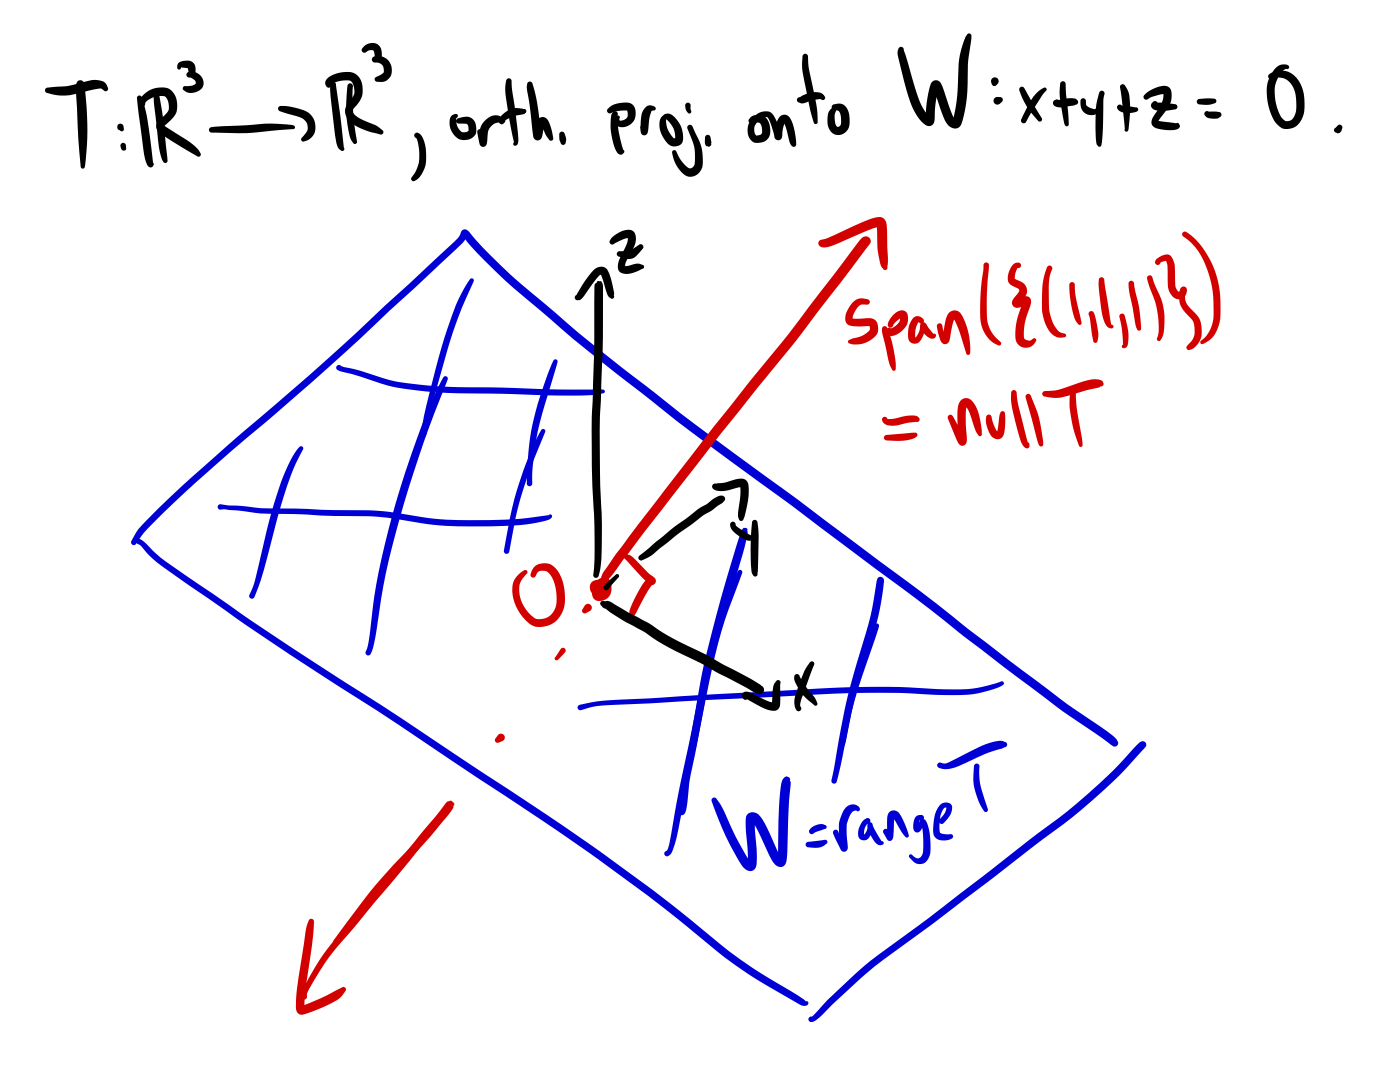
\includegraphics[width=2.5in]{Images/OrthoRankNull}
\]
  \end{example}
\end{frame}
\begin{frame}
 \begin{example}
 Define $T\colon M_{nn}\rightarrow M_{nn}$ as $T(A)=A^T-A$. 
 \bspace 
 As we have seen elsewhere, $\NS T=\{A\in M_{nn}\colon A^T=A\}$ and $\range T=\{A\in M_{nn}\colon A^T=-A\}$, the space of symmetric and skew-symmetric matrices, respectively.  
 \bpause 
 As we have also seen, the dimension of the space of symmetric matrices is $\frac{n(n+1)}{2}$, and the dimension of skew-symmetric matrices is $\frac{n(n-1)}{2}$. 
 \bspace
 According to the rank-nullity theorem we must have 
 \begin{align*}
 n^2&=M_{nn}\\
 &=\dim\NS T+\dim\range T\\
 &=\frac{n(n+1)}{2}+\frac{n(n-1)}{2}.
 \end{align*}
 We have thus given a linear algebraic proof of the identity $n^2=\frac{n(n+1)}{2}+\frac{n(n-1)}{2}$. 
 \bpause
 Yes, there is a more straightforward arithmetic proof, but you must admit this one is pretty cool, and it illustrates how results in one area of mathematics (e.g., linear algebra) can sometimes be translated into results in a completely different area (e.g., combinatorics). 
 
 \end{example}
\end{frame}
\begin{frame}{Relative sizes of $\NS T$ and $\range T$}
Let $T\colon V\rightarrow W$, where $\dim V=n$. Since 
$
\dim\NS T+\dim\range T=n,
$
we see that the {\color{red} bigger} the null space (dimension-wise), the {\color{blue} smaller} the range, and vice versa. 

Let's see this numerically in action. Assume $T\colon V\rightarrow W$ is linear. 
\bb
\pause\ii Suppose $\dim V=5$ and $\dim W=3$. Prove: $\NS T$ is nontrivial. 
\bpause
If $\NS T=\{\boldzero\}$, then $\dim\range T=5-0=5$; but this is impossible since $\range T\subseteq W$ and $\dim W=3$. Thus $\NS T\ne \{\boldzero\}$; i.e., there is a nonzero $\boldv\in\NS T$. This shows $\NS T$ is nontrivial. 
\pause\ii Suppose $\dim V=7$, $\dim W=5$, and $\dim\NS T=2$. Prove: $\range T= W$. 
\bpause 
We have $\dim\range T=7-\dim\NS T=7-2=5$. Since $\range T\subseteq W$ and $\dim\range T=\dim W$, we conclude $\range T=W$. 
\ee
\end{frame}

\begin{frame}{Fundamental subspaces of a matrix}
When $T=T_A$ for some $m\times n$ matrix $A$, we can develop a systematic way of computing bases for $\NS A$ and $\range A$. Not surprisingly this procedure involves Gaussian elimination, as we will outline below. 
\bspace 
In fact the procedure allows us to compute bases for the three following subspaces associated to a matrix, the so-called \alert{fundamental subspaces} of $A$. 

\pause
\begin{definition}
Let $A$ be a an $m\times n$ matrix with rows $\boldr_1,\dots, \boldr_m$ and columns $\boldc_1,\dots \boldc_n$. The following subspaces are called the {\bf fundamental subspaces of $A$}. 
\bb
\ii The {\bf null space} of $A$ is defined as 
\[
\NS A =\{\boldx\in\R^n\colon A\boldx=\boldzero\}\subset \R^n.
\]
\ii The {\bf row space} of $A$ is defined as 
\[
\RS A =\Span(\{\boldr_1,\dots, \boldr_m\})\subset\R^n.
\]
\ii The {\bf column space} of $A$ is defined as 
\[
\CS A=\Span(\{\boldc_1,\dots \boldc_n\})\subset\R^m. 
\]
\ee
\end{definition}
\pause 
The careful reader will object that $\range A$ does not appear on this list! Fear not, as we show in the next slide \alert{$\CS A=\range A$}. 
\end{frame}

\begin{frame}{$\CS A=\range A$}
Take an $m\times n$ matrix and consider $A$ as a collection of $n$ columns $\boldc_j$, each of which lives in $\R^m$:
\[
A=\begin{bmatrix}
\vert&\vert& \cdots &\vert\\
\boldc_1&\boldc_2&\cdots &\boldc_n\\
\vert&\vert& \cdots &\vert
\end{bmatrix}
\]
\pause
Then we have 
\begin{eqnarray*}
\boldb\in\CS A &\Leftrightarrow& \boldb\in\Span(\{\boldc_1,\dots,\boldc_n\})\\
\pause&\Leftrightarrow & \boldb=a_1\boldc_1+a_2\boldc_2+\cdots + a_n\boldc_n \text{ for some $a_i$}\\
\pause&\Leftrightarrow & \boldb=A\begin{bmatrix}
a_1\\ a_2\\ \vdots \\ a_n
\end{bmatrix} \text{ (by column expansion!!)} \\
\pause&\Leftrightarrow & \text{ there is an $\boldx\in\R^n$ such that } A\boldx=\boldb \\
\pause&\Leftrightarrow &\boldb\in \range A.
\end{eqnarray*}
We conclude:
\[
\boxed{\CS A=\range A}
\]
\end{frame}

\begin{frame}{Computing the fundamental spaces}
\footnotesize
Once again Gaussian elimination is the main tool for computing fundamental spaces: start with $A$, row reduce to $U$, compute the fundamental spaces of $U$. However, there are some subtleties involved. Here is the overall description for how to proceed:
\[
\pause 
\begin{array}{lcl}
\text{Space}&\text{Relation}&\text{How to pick a basis}\\
\hline
\text{Null space}&\NS A=\NS U&\left(\begin{array}{c}\text{find vector parametrization}\\ \text{of solutions to $U\boldx=\boldzero$} \end{array}\right) \\
\\
\pause\text{Row space}&\RS A=\RS U &\left(\begin{array}{c}\text{nonzero rows of $U$ }\\ \text{form a basis of $\RS(A)$} \end{array}\right) \\
\\
\pause\text{Column space}&\CS A \alert{\ne}\CS U &\left(\begin{array}{c}\text{pick columns of $A$ corresponding}\\ \text{to columns of $U$ with leading 1's} \end{array}\right) 
\end{array}
\]
\end{frame}
\begin{frame}
Let's prove some of the previous claims. We will begin by proving the following more general result.
\bspace
\alert{Claim}. If $A$ and $B$ are \alert{row equivalent}, then $\NS(A)=\NS(B)$, $\RS(A)=\RS(B)$, and if a certain subset of the columns of $B$ form a basis of $\CS(B)$, then the same is true of the corresponding columns of $A$ and $\CS(A)$. 
\pause
\begin{proof}
First observe that $A$ is row equivalent to $B$ iff $(E_rE_{r-1}\cdots E_1)A=B$ for some elementary matrices $E_i$ iff $QA=B$ for some invertible $Q$. (The latter ``iff" follows since the $E_i$ are elementary, and since all invertible matrices are products of elementary matrices. )
\pause
So we assume $QA=B$ for some invertible $Q$. 
\bpause 
\alert{Null space}. We have shown in an exercise that $A\boldx=\boldzero$ iff $QA\boldx=\boldzero$ iff $B\boldx=\boldzero$. It follows that $\NS(A)=\NS(B)$. 
\bpause
\alert{Row space}
To show $\RS(A)=\RS(B)$, it is enough to show that $\RS(B)\subseteq \RS(A)$; this is because we can then apply the same reasoning using the fact that $A=Q^{-1}B$, $Q^{-1}$ invertible. \pause The row method tells us that each row of $B=QA$ is a linear combination of the rows of $A$. Thus each row of $B$ lies in $\RS(A)$, the span of the rows of $A$. \pause But then we must have $\RS(B)\subseteq\RS(A)$, since $\RS(B)$ is the ``smallest" subspace containing all rows of $B$ (by properties of span).
\bpause
\alert{Column space} (Sketch). Here one can show that columns $\boldc_{i_1}, \boldc_{i_2},\dots, \boldc_{i_r}$ of $A$ form a basis of $\CS(A)$ iff $Q\boldc_{i_1}, Q\boldc_{i_2},\dots, Q\boldc_{i_r}$ form a basis of $\CS(B)$. By the column method the vectors $Q\boldc_{i_j}$ are precisely the corresponding columns of $B=QA$. 
\end{proof}

\end{frame}
\begin{frame}{Example}
\footnotesize
Let's compute bases/dimensions for the fundamental spaces of \\ 
$A=\begin{bmatrix}[rrrr]
2&2&4&2\\
6&6&11&5\\
-4&-4&-7&-3
\end{bmatrix}
$.\\
\pause $A$ reduces to the matrix 
$U=\begin{bmatrix}[rrrr]
1&1&2&1\\
0&0&1&1\\
0&0&0&0
\end{bmatrix}
$
\bpause
First compute 
\[
\NS(U)=\{(s-r,r,-s,s)\colon r, s\in\R\}=\{s(1,0,-1,1)+r(-1,1,0,0)\colon r,s\in\R\}.
\]
It follows that $\NS A=\NS U=\Span \{(1,0,-1,1), (-1,1,0,0)\}$, and thus that $B=\{(-1,1,0,0), (1,0,-1,1)\}$ is a basis for $\NS(A)$. We conclude $\dim\NS A=2$. 
\bpause Next, the rank-nullity theorem implies $\dim\range U=\dim \R^4-\dim\NS U=2$. Thus to choose a basis for $\CS U=\range U$ we need only pick two linearly independent columns of $U$:  the first and third columns will do. It follows that the first and third columns of $A$ form a basis for $\CS A$. This gives us $B''=\{(2,6,-4), (4,11,-7)\}$ as a basis for $\CS A $. 
\bpause
Finally, we have $\RS A =\RS U$, and clearly we can take the nonzero rows of $U$ as a basis for this. Thus $B'=\{(1,1,2,1),(0,0,1,1)\}$ is a basis for $\RS A $. We conclude $\dim\RS A=2$. 
\end{frame}
\begin{frame}
 The preceding example nicely illustrates our general procedure for computing bases for the fundamental spaces of $A$. 
 \begin{block}{Computing bases for the fundamental spaces}
\bb[(i)]
\ii Reduce $A$ to row echelon form matrix $U$. 
\ii $\boxed{\NS(A)=\NS(U)}$. Use free/leading variable method to give full description of solutions $U\boldx=\boldzero$. Extract a basis from the resulting parametric description. 
\ii $\boxed{\RS(A)=\RS(U)}$. A basis for $\RS(U)$ (and hence $\RS(A)$) consists of the nonzero rows of $U$. 
\ii $\boxed{\CS(A)\ne \CS(U)}$. The columns of $U$ with leading 1's are a basis for $\CS(U)$. The {\em corresponding columns} of $A$ form a basis for $\CS(A)$. 
\ee
\end{block}
\pause
\begin{comment}
It is clear that the nonzero rows of $U$ form a basis of $\RS U$: the staircase pattern of leading 1's guarantees they are linearly independent, and we can obviously discard the zero rows. 
\bpause
It is not difficult to show that the columns of $U$ with leading 1's are linearly independent. (Exercise!) That they are in fact a basis follows from the fact that $\#\text{(leading 1's)}=n-\#\text{(free variables)}=n-\dim\NS U=\dim\CS U$. 
\end{comment}
\end{frame}
\begin{frame}{Rank-nullity theorem for matrices}
The previous discussion gives us a much more detailed analysis of the spaces involved in the rank-nullity theorem in the special case where $T=T_A$. We collect some of those details here. 
\begin{block}{Rank-nullity theorem for matrices}
Let $A$ be $m\times n$. Suppose $A$ is row equivalent to the row echelon matrix $U$. 
\bb
\ii $\CS A=\range A$
\ii $\dim\NS A=\#(\text{free variables in the system $U\boldx=\boldzero$})$
\ii $\rank A=\dim\CS A=\dim\RS A=\#(\text{leading 1's in $U$})$
\ii $\rank A\leq \min\{m,n\}$. (Since $\#(\text{leading 1's in $U$})\leq m$ and $\#(\text{leading 1's in $U$})\leq n$.) 
\ii $n=\dim\NS A+\dim\CS A=\dim\NS A+\dim\RS A$. 
\ee
\end{block}
\end{frame}
\begin{frame}{Extending/contracting sets to bases}
Recall that if $\dim V=n$, then any linearly independent set can be \alert{extended} to a basis of $B$, and any spanning set can be \alert{contracted} to a basis. 

In the special case when $V=\R^n$, our fundamental space algorithms provide a means of performing these extensions/contractions. \bpause
Let $\boldv_1,\boldv_2, \dots, \boldv_r\in \R^n$. 
\bb
\ii \alert{Extending to basis}. If the $\boldv_i$ are independent, then to extend to a basis of $\R^n$ proceed as follows:
\bb
\ii Build the matrix $A$ whose columns (in order) are $\boldv_1,\boldv_2, \dots, \boldv_r, \bolde_1,\bolde_2,\dots, \bolde_n$.
\ii Apply the column space algorithm to $A$. 
\ee
\ii \alert{Contracting to basis}. If the $\boldv_i$ span the subspace$W\subseteq\R^n$, then to contract to a basis of $W$ proceed as follows:
\bb
\ii Build the matrix $A$ whose columns are $\boldv_1, \boldv_2, \dots, \boldv_r$. 
\ii Apply the column space algorithm to $A$. 
\ee


\ee
\end{frame}
\begin{frame}{Example}
\footnotesize
Let $W=\Span\{\boldv_1,\boldv_2, \boldv_3, \boldv_4, \boldv_5\}$ where 
\[
\begin{array}{ll}
\boldv_1=(1,-1,5,2)&\boldv_2=(-2,3,1,0)\\
\boldv_3=(4,-5,9,4)&\boldv_4=(0,4,2,-3)\\
\boldv_5=(-7,18,2,-8)
\end{array}
\]
Find a subset of the $\boldv_i$ that yields a basis of $W$. 
\bpause 
We know the $\boldv_i$ span $W$, so to get a basis we need to ``throw out the redundant ones". To figure out which ones need to go, we create a matrix $A$ by setting the $\boldv_i$ as  its \alert{columns} (not its rows)! The procedure for finding a basis for $\CS(A)$ then gives us a subset of these columns that forms a basis.
\bpause 
$A=\begin{bmatrix}[rrrrr]
1&-2&4&0&-7\\
-1&3&-5&4&18\\
5&1&9&2&2\\ 
2&0&4&-3&-8
\end{bmatrix}
\xrightarrow[]{\text{row red.}}
U=
\begin{bmatrix}[rrrrr]
\boxed{1}&0&2&0&-1\\
0&\boxed{1}&-1&0&3\\
0&0&0&\boxed{1}&2\\
0&0&0&0&0
\end{bmatrix}
$
\bpause
It follows that $\{\boldv_1,\boldv_2, \boldv_4\}$ is a basis for $W$. 
\end{frame}
\begin{frame}{Example}
Extend the set $S=\{ (1,1,1,1), (-2,-2,3,3)\}$ to a basis of $\R^4$. 
\bpause
Take the matrix 
\[
A=\begin{bmatrix}
1&-2&1&0&0&0\\
1&-2&0&1&0&0\\
1&3&0&0&1&0\\
1&3&0&0&0&1
\end{bmatrix}
\]
This matrix row reduces to 
\[
U=\begin{bmatrix}
\boxed{1}&-2&1&0&0&0\\
0&\boxed{1}&-1/5&0&1/5&0\\
0&0&\boxed{1}&-1&0&0\\
0&0&0&0&\boxed{1}&-1
\end{bmatrix}
\]
\pause
It follows that the first, second, third and fifth column of $A$ form a basis of $\CS(A)=\R^4$. Thus 
\[
B=\{(1,1,1,1), (-2,-2,3,3), (1,0,0,0), (0,0,1,0)\}
\]
is a basis of $\R^4$ extending $S$. 

\end{frame}
%\begin{frame}{Working in other spaces $V$}
%These algorithms gives us means of computing bases for subspaces inside $\R^n$. What about more exotic vector spaces, like $P_n$, $M_{mn}$, etc.? 
%\bspace 
%The trick when working in one of these more abstract spaces is to first pick a basis $B$ of $V$ (oftentimes the ``standard" one), and use the coordinate vector operator 
%\[
%\boldv\mapsto [\boldv]_B\in\R^n
%\]
%to translate the problem into a question about vectors in $\R^n$. 
%\bpause Use one of the previous algorithms to solve the corresponding problem in $\R^n$, then translate your results back in terms of the original vector space $V$. 
%\bspace The following examples illustrate this technique. 
%\end{frame}
%\begin{frame}{Example}
%Let $W=\Span\{p_1,p_2, p_3, p_4, p_5\}\subset P_3$ where 
%\[
%\begin{array}{ll}
%p_1=1-x+5x^2+2x^3&p_2=-2+3x+x^2\\
%p_3=4-5x+9x^2+4x^3&p_4=4x+2x^2-3x^3\\
%p_5=-7+18x+2x^2-8x^3
%\end{array}
%\]
%Find a subset of the $p_i$ that yields a basis of $W$. 
%\bpause 
%Let $B=\{1,x,x^2, x^3\}$ be the standard basis for $P_3$. Apply $[\hspace{10pt}]_B$ to each of the $p_i$ to get the exact same vectors $\boldv_i$ from the previous example.
%\bpause As we saw in that example, our column space algorithm showed that $\boldv_1, \boldv_2$ and $\boldv_4$ formed a basis for the span of the $\boldv_i$. 
%\bpause 
%It follows that $\{p_1, p_2, p_4\}$ is a basis for $W$ inside $P_3$.
% 
%\end{frame}
%\begin{frame}{Example}
%Let $A_1=\begin{bmatrix}[rr]
%1&1\\-2&0
%\end{bmatrix}
%$,
%$A_2=\begin{bmatrix}[rr]
%1&-1\\-1&1
%\end{bmatrix}
%$,
%$A_3=\begin{bmatrix}[rr]
%1&1\\1&-3
%\end{bmatrix}
%$, and let $W=\Span(\{A_1,A_2,A_3\})$. 
%
%Decide whether $A=\begin{bmatrix}
%1&0\\-1&0
%\end{bmatrix}
%$
%is in $W$. 
%\bpause
%Let $B$ be the standard basis of $M_{22}$. Translate everything to $\R^4$ using $(\underline{\hspace{.2cm}})_B$. 
%\bspace We are then asking whether $\boldv=(1,0,1,0)$ is in the span of $\boldv_1=(1,1,-2,0)$, $\boldv_2=(1,-1,-1,1)$, $\boldv_3=(1,1,1,-3)$. This is equivalent to whether the matrix equation 
%\[
%\begin{bmatrix}[rrr]
%1&1&1\\
%1&-1&1\\
%-2&-1&1\\
%0&1&-3
%\end{bmatrix}
%\boldx
%=\begin{bmatrix}[r]
%1\\ 0\\-1 \\0 
%\end{bmatrix}
%\] 
%has a solution. 
%
%GE shows that in fact we can solve this. (Do it!) This means $\boldv$ is a linear combination of the $\boldv_i$, and thus that $A$ is a linear combination of the $A_i$. 
%
%We conclude $A\in W$. 
%\end{frame}


%\begin{corollary}[Corollary of R-N]
%Let $A$ be $m\times n$. 
%\bb[(i)]
%\pause\ii If $m>n$, then there is a $\boldb\in\R^m$ such that $A\boldx=\boldb$ has no solution (i.e., is inconsistent). 
%\ii If $m<n$, then there is a nontrivial $\boldx\ne\boldzero_n\in\R^n$ such that $A\boldx=\boldzero_m$. 
%\ee
%\pause
%\begin{proof}
%\ \\
%(i) If $m>n$, then $\dim(\CS(A))=\dim(\RS(A))\leq n<m$. Thus $\CS(A)\ne\R^m$, which means there is a $\boldb$ such that $A\boldx=\boldb$ has no solution. 
%\bpause
%(ii) If $m<n$, then $\dim(\CS(A))\leq m<n$. By the R-N theorem we have 
%\[
%\dim(\NS(A))=n-\dim(\CS(A))>n-n=0.
%\]
%Thus $\NS(A)$ is a nontrivial space, which means there is a $\boldx\ne\boldzero_n$ with $A\boldx=\boldzero_m$. 
%\end{proof}
%\end{corollary}
%\end{frame}
\begin{frame}{Invertibility Theorem}
\alert{Suppose $A$ is a square $n\times n$ matrix} . Recall that $A$ is invertible if and only if $A\boldx=\boldzero$ has a unique solution. This is equivalent to $\NS(A)=\{\boldzero\}$. Thus we have: 
\[
A \text{ invertible } \Leftrightarrow \NS(A)=\{\boldzero\}\Leftrightarrow \nullity(A)=0.
\]
\pause Similarly, we have $A$ invertible if and only if $A\boldx=\boldb$ has a solution \alert{for all} $\boldb\in\R^n$. As we saw earlier, $\CS(A)=\{\boldb\in\R^n\colon A\boldx=\boldb \text{ has a solution}\}$. Thus we see that 
\[
A \text{ invertible}\Leftrightarrow \CS(A)=\R^n \Leftrightarrow \rank(A)=n \Leftrightarrow \RS(A)=\R^n,
\]
where the last equivalence follows since $\RS(A)\subset\R^n$ and $\dim(\RS(A))=n$. 
\bpause 
Looks like we have quite a few new statements to add to our Invertibility Theorem! 
\end{frame}
\begin{frame}
\begin{theorem}[Invertibility theorem]
Let $A$ be $n\times n$. The following statements are equivalent. 
\bb[(a)]
\ii $A$ is invertible.
\ii $A\boldx=\boldzero$ has a unique solution (the trivial one). 
\ii $A$ is row equivalent to $I_n$, the $n\times n$ identity matrix.
\ii $A$ is a product of elementary matrices. 	
\ii $A\boldx=\boldb$ has a solution for every $n\times 1$ column vector $\boldb$. 
\ii $A\boldx=\boldb$ has a {\em unique} solution for every $n\times 1$ column vector $\boldb$. 
\ii $\det A\ne 0$.
\ii $\NS A=\{\boldzero\}$.
\ii $\nullity A=0$.
\ii $\rank A=n$. 
\ii $\CS A=\R^n$.
\ii $\RS A=\R^n$.
\ii The columns of $A$ are linearly independent (or span $\R^n$, or are a basis of $\R^n$).
\ii The rows of $A$ are linearly independent (or span $\R^n$, or are a basis of $\R^n$). 
\ee
\end{theorem}

\end{frame}








\setcounter{exercises@solutionnumber}{1}
\ \\
\section*{4.3: coordinate vectors} \phantomsection \label{S:basissection}
\bb
\ii Find the coordinate vector $[\boldv]_B$ relative to the basis $B= {\boldv_1,\boldv_2,\boldv_3}$ for $\R^3$.
\bb
\ii $\boldv =(2,-1,3)$; $\boldv_1 = (1,0,0)$, $\boldv_2=(2,2,0)$, $\boldv_3 = (3,3,3)$
\ii $\boldv =(5,-12,3)$; $\boldv_1 = (1,2,3)$, $\boldv_2=(-4,5,6)$, $\boldv_3 = (7,-8,9)$
\ee
\begin{solution}
\noindent In both parts, the coordinate vector $[\boldv]_S$ is computed by finding $c_1,c_2,c_3$ such that $\boldv=c_1\boldv_1+c_2\boldv_2+c_3\boldv_3$. We do so using GE. 
\noindent (a) 
$$
\begin{bmatrix}[rrrr]
1&2&3&2\\
0&2&3&-1\\
0&0&3&3
\end{bmatrix}
$$
\begin{eqnarray*}
c_3 &=& 1\\
c_2 &=& -1/2 -3/2 = -2\\
c_1 &=& 2-3+4 = 3
\end{eqnarray*}
Thus $[\boldv]_B=(3,-2,1)$.
\\
(b) 
\begin{eqnarray*}
\begin{bmatrix}[rrrr]
1&-4&7&5\\
2&5&-8&-12\\
3&6&9&3
\end{bmatrix}
&\xrightarrow[]{2r_1-r_2}&
\begin{bmatrix}[rrrr]
1&-4&7&5\\
0&-13&22&22\\
3&6&9&3
\end{bmatrix}\\
&\xrightarrow[]{3r_1-r_3}&
\begin{bmatrix}[rrrr]
1&-4&7&5\\
0&-13&22&22\\
0&-18&12&12
\end{bmatrix}\\
&\xrightarrow[]{-1/13r_2}&
\begin{bmatrix}[rrrr]
1&-4&7&5\\
0&1&-22/13&-22/13\\
0&-18&12&12
\end{bmatrix}\\
&\xrightarrow[]{18r_2+r_3}&
\begin{bmatrix}[rrrr]
1&-4&7&5\\
0&1&-22/13&-22/13\\
0&0&-240/13&-240/13
\end{bmatrix}\\
&\xrightarrow[]{-13/240r_3}&
\begin{bmatrix}[rrrr]
1&-4&7&5\\
0&1&-22/13&-22/13\\
0&0&1&1
\end{bmatrix}\\
\end{eqnarray*}
\begin{eqnarray*}
c_3 &=& 1\\
c_2 &=& -22/13 + 22/13 = 0\\
c_1 &=& 5 - 7 = -2
\end{eqnarray*}
Thus the coordinate vector is $[\boldv]_B=(-2,0,1)$.
\end{solution}
\ii Find the coordinate vector $[p]_B$ relative to the basis $B= \{p_1,p_2,p_3\}$ for $P_2$.
\bb
\ii $p = 4 -3x +x^2$, $p_1 = 1$, $p_2 = x$, $p_3 = x^2$
\ii $p = 2 -x +x^2$, $p_1+x = 1$, $p_2 = 1+x^2$, $p_3 = x+x^2$
\ee
\begin{solution}
\noindent In both parts, the coordinate vector $[\boldv]_B$ is computed by finding $c_1,c_2,c_3$ such that $p=c_1p_1+c_2p_2+c_3p_3$. As usual this boils down (after grouping like terms and equating like coefficients) to solving a certain linear system, which we do either by inspection, or by using GE. 
\\
(a)  By inspection, we see that $p=4p_1+(-3)p_2+p_3$. Thus $[p]_B=(4,-3,1)$. 
\\
(b) We solve the corresponding linear system in this case using GE:
\begin{eqnarray*}
\begin{bmatrix}[rrrr]
1&1&0&2\\
1&0&1&-1\\
0&1&1&1
\end{bmatrix}
&\xrightarrow[]{r_2\leftrightarrow r_3}&
\begin{bmatrix}[rrrr]
1&1&0&2\\
0&1&1&1\\
1&0&1&-1
\end{bmatrix}\\
&\xrightarrow[]{r_1 -r_3}&
\begin{bmatrix}[rrrr]
1&1&0&2\\
0&1&1&1\\
0&1&-1&3
\end{bmatrix}\\
&\xrightarrow[]{r_2 -r_3}&
\begin{bmatrix}[rrrr]
1&1&0&2\\
0&1&1&1\\
0&0&2&-2
\end{bmatrix}\\
\end{eqnarray*}
\begin{eqnarray*}
c_3 &=& -1\\
c_2 &=& 1 + 1 = 2\\
c_1 &=& 2-2 = 0
\end{eqnarray*}
Thus the coordinate vector is $[p]_B=(0,2,-1)$.
\end{solution}
\ii The set $B = \{A_1,A_2,A_3,A_4\}$ is a basis for $M_{22}$, where 
$$
A_1 =
\begin{bmatrix}[rr]
1&0\\
1&0
\end{bmatrix}
, A_2=
\begin{bmatrix}[rr]
1&1\\
0&0
\end{bmatrix}
, A_3 = 
\begin{bmatrix}[rr]
1&0\\
0&1
\end{bmatrix}
, A_4 = 
\begin{bmatrix}[rr]
0&0\\
1&0
\end{bmatrix}
$$
(a) Compute $[A]_B$, where $$A = 
\begin{bmatrix}[rr]
6&2\\
5&3
\end{bmatrix}.$$
\vspace{.1in}
\\
(b) Now compute $[A]_B$ for the general matrix 
\[
A=
\begin{bmatrix}
a&b\\ c&d
\end{bmatrix}.
\]
\begin{solution}
\noindent
(a) Finding $c_1, c_2, c_3, c_4$ such that $A=c_1A_1+c_2A_2+c_3A_3+c_4A_4$ amounts to solving the system corresponding to the augmented matrix below:
$$
\begin{bmatrix}[rrrr|r]
1&1&1&0&6\\
0&1&0&0&2\\
1&0&0&1&5\\
0&0&1&0&3
\end{bmatrix}
$$,
or equivalently, the matrix equation 
\[
\underset{A}{\underbrace{\begin{bmatrix}
1&1&1&0\\
0&1&0&0\\
1&0&0&1\\
0&0&1&0
\end{bmatrix}}}
\begin{bmatrix}
c_1\\ c_2\\ c_3\\ c_4
\end{bmatrix}=
\begin{bmatrix}
6\\ 2\\ 5\\ 3
\end{bmatrix}
\]
After GE this reduces to 
\[
\begin{bmatrix}[rrrr|r]
1&1&1&0&6\\
0&1&0&0&2\\
0&0&1&-1&-1\\
0&0&0&1&4
\end{bmatrix}
\]
Thus
\begin{eqnarray*}
c_4 &=& 4\\
c_3 &=& 3\\
c_2 &=& 2\\
x_1 &=& 1
\end{eqnarray*}
Then $A = 1A_1 + 2A_2 +3A_3 +4A_4$ and the coordinate vector is:\\ $[A]_B = (1,2,3,4)$.
\vspace{.1in}
\\
(b) For the general matrix $\begin{bmatrix}
a&b\\c&d
\end{bmatrix}$, the same reasoning shows that we need to solve the matrix equation 
\[
\underset{A}{\underbrace{\begin{bmatrix}
1&1&1&0\\
0&1&0&0\\
1&0&0&1\\
0&0&1&0
\end{bmatrix}}}
\begin{bmatrix}
c_1\\ c_2\\ c_3\\ c_4
\end{bmatrix}=
\begin{bmatrix}
a\\ b\\ c\\ d
\end{bmatrix}
\]
We could proceed exactly as above, using Gaussian elimination. Instead, I observe that $A$ is invertible, and solve (after computing $A^{-1}$) 
\begin{align*}
\begin{bmatrix}
c_1\\ c_2\\ c_3\\ c_4
\end{bmatrix}&=A^{-1}\begin{bmatrix}
a\\ b\\ c\\ d
\end{bmatrix}\\
&=\begin{bmatrix}[rrrr]
1& -1& 0& -1\\ 0& 1& 0& 0\\ 0& 0& 0& 1\\ -1& 1& 1& 1
\end{bmatrix}\begin{bmatrix}
a\\ b\\ c\\ d
\end{bmatrix}\\
&=\begin{bmatrix}
a - b - d\\ b\\ d \\ -a + b + c + d
\end{bmatrix}
\end{align*}
Thus for general $A=\begin{bmatrix}
a&b\\ c&d
\end{bmatrix}$ we see that 
\[
[A]_B=(a-b-d, b, d, -a+b+c+d)
\]
\end{solution}
\begin{samepage}
\ii Suppose $\dim(V)=n$, and let $B=\{\boldv_1,\dots ,\boldv_n\}$  be a basis for $V$. 
Define 
\begin{align*}
T\colon V&\rightarrow \R^n\\
\boldv&\mapsto [\boldv]_B.
\end{align*}
Prove all statements of the coordinate vector map theorem, as listed below. 
\bb
\ii  $T$ is a linear transformation. 

\ii $T(\boldv_1)=T(\boldv_2)$ if and only if $\boldv_1=\boldv_2$: i.e., $T$ is {\em one-to-one}. 

In particular, $T(\boldv)=\boldzero$ if and only if $\boldv=\boldzero_V$. 

\ii  $\range T=\R^n$: i.e. $T$ is {\em onto}. 

\ii  A set $S=\{w_1,w_2,\dots, w_r\}\subseteq V$ is linear independent  if and only if $T(S)=\{T(\boldw_1), T(\boldw_2),\dots, T(\boldw_r)\}\subseteq \R^n$ is linearly independent. 

\ii A set $S=\{w_1,w_2,\dots, w_r\}\subseteq V$ spans $V$ if and only if $T(S)=\{T(\boldw_1), T(\boldw_2),\dots, T(\boldw_r)\}$ spans $\R^n$. 
\ee
\end{samepage}
\begin{solution}
\noindent (a) We must show $[c\boldv+d\boldw]_B=c[\boldv]_B+d[\boldw]_B$ for all $\boldv,\boldw\in V$ and all $c,d\in\R$. 
To this end, given $\boldv, \boldw$, write
\begin{align*}
\boldv&=a_1\boldv_1+a_2\boldv_2+\cdots +a_n\boldv_n\\
\boldw&=b_1\boldv_1+b_2\boldv_2+\cdots +b_n\boldv_n
\end{align*} 
We can do this since $B$ spans $V$. It follows that for any $c,d\in\R$ 
\[
c\boldv+d\boldw=(ca_1+db_1)\boldv_1+(ca_2+db_2)\boldv_2+\cdots +(ca_n+db_n)\boldv_n
\]
Now, using the definition of coordinate vectors we have 
\begin{align*}
[c\boldv+d\boldw]_B&=\colvec{ca_1+db_1\\ca_2+db_2\\ \vdots \\ ca_n+db_n}\\
&=\colvec{ca_1\\ca_2\\ \vdots \\ ca_n}+\colvec{db_1\\db_2\\ \vdots \\ db_n}\\
&=c\colvec{a_1\\a_2\\ \vdots \\ a_n}+d\colvec{b_1\\b_2\\ \vdots \\ b_n}\\
&=c[\boldv]_B+d[\boldw]_B.
\end{align*} 
(b) I begin, somewhat ponderously, by first proving that $T(\boldv)=[\boldv]_B=(0,0,\dots, 0)$ if and only if $\boldv=\boldzero$. 
This is fairily obvious. Indeed, given an arbitrary $\boldv\in V$, we have $\boldv=c_1\boldv_1+c_2\boldv_2+\cdots +c_n\boldv_n$ for some $c_i\in \R$, and $[\boldv]_B=(c_1,c_2,\dots, c_n)$.  Clearly $[\boldv]_B=(0,0,\dots, 0)$ if and only if $c_1=c_2=\cdots =c_n=0$ if and only if $\boldv=\boldzero$. 

We have proved a special case of the general claim: namely $T(\boldv)=T(\boldzero)$ iff $\boldv=\boldzero$. The general case follows by using the fact that $T$ is linear. We have 
\begin{align*}
T(\boldv_1)=T(\boldv_2)&\Leftrightarrow T(\boldv_1)-T(\boldv_2)=(0,0,\dots, 0)\\
&\Leftrightarrow T(\boldv_1-\boldv_2)=(0,0,\dots, 0) &\text{($T$ is linear)}\\
&\Leftrightarrow \boldv_1-\boldv_2=\boldzero &\text{(by our special case!)}\\
&\Leftrightarrow \boldv_1=\boldv_2
\end{align*}
This same trick can be used to show, in general, that a linear transformation $T$ is one-to-one if and only if $\NS T=\{\boldzero\}$.
\\
(c) This is obvious. Given any $(c_1,c_2,\dots, c_n)\in\R^n$, set $\boldv=c_1\boldv_1+c_2\boldv_2+\cdots +c_n\boldv_n$. Then by definition $[\boldv]_B=(c_1,c_2,\dots, c_n)$. 
\\
(d) We can now use our results above to prove the remaining statements. Note that 
\begin{align*}
c_1\boldw_1+c_2\boldw_2+\cdots +c_r\boldw_r=\boldzero &\Leftrightarrow T(c_1\boldw_1+c_2\boldw_2+\cdots +c_r\boldw_r)=(0,0,\dots, 0) &\text{(special case of (b)!)}\\
&\Leftrightarrow c_1T(\boldw_1)+c_2T(\boldw_2)+\cdots +c_rT(\boldw_r)=(0,0,\dots, 0) &\text{($T$ is linear)}
\end{align*}
From this we see that the $\boldw_i$ are linearly independent if and only if the $T(\boldw_i)$ are linearly independent. 
\\
(e) Suppose the $\boldw_i$ span. Given any $\boldy\in \R$, there is a $\boldv\in V$ such that $T(\boldv)=\boldy$, since $\range T=\R^n$ (part (c)). Since the $\boldw_i$ span, we can write $\boldv=d_1\boldw_1+d_2\boldw_2+\cdots +d_r\boldw_r$. Then 
\[
\boldy=T(\boldv)=T(d_1\boldw_1+d_2\boldw_2+\cdots +d_r\boldw_r)=d_1T(\boldw_1)+d_2T(\boldw_2)+\cdots +d_rT(\boldw_r),\]
showing that the $T(\boldw_i)$ span $\R^n$. 

Conversely, suppose the $T(\boldw_i)$ span $\R^n$. Given any $\boldv\in V$, we have $T(\boldv)=d_1T(\boldw_1)+d_2T(\boldw_2)+\cdots +d_rT(\boldw_r)$, for some $d_i\in\R$, since $T(\boldv)\in\R^n$ and the $T(\boldw_i)$ span $\R^n$ by assumption. But then 
\[
T(\boldv)=T(d_1\boldw_1+d_2\boldw_2+\cdots +d_r\boldw_r),
\]
since $T$ is linear. It follows that 
\[
\boldv=d_1\boldw_1+d_2\boldw_2+\cdots +d_r\boldw_r,
\]
since $T$ is 1-1 by (b) !! This shows that the $\boldw_i$ span $V$, as desired. 
\\
Note: properties (d) and (e) can be summarized by saying $T$ preserves linear independence and $T$ preserves spanning sets. This property is enjoyed more generally by any isomorphism between vector spaces. 

\end{solution}
\ii Let $S=\{p_1=1+x+2x^2,p_2=1-x,p_3=1+x^2,p_4=1+x-x^2\}$ and let $W=\Span(S)\subset P$.  (Recall $P$ is the space of all polynomials.) 
\bb
\ii Use ``street smarts" to decide whether $S$ is linearly independent. 
\ii Use coordinate vectors and an appropriate fundamental space algorithm to choose a basis of $W=\Span(S)$ {\em from among the elements of $S$}.
\ii Give a satisfying description of $W$. 
\ee
\begin{solution}
\noindent 
(a) In fact we see that $S$ lies within the smaller subspace $P_2$, which has dimension $3$. Since $S$ has 4 elements and lives in a 3-dimensional space, it is guaranteed to be dependent. Street smarts! 
\\ \\
(b) Let $B$ be the standard basis of $P_2$: i.e., $B=\{1,x,x^2\}$. Then we can translate this whole problem into $\R^3$ using coordinate vectors. Namely we let:
\[
\boldv_1=(p_1)_B=\begin{bmatrix}
1\\ 1\\ 2
\end{bmatrix}, \boldv_2=(p_2)_B=\begin{bmatrix}
1\\ -1\\ 0
\end{bmatrix}, \boldv_3=(p_3)_B=\begin{bmatrix}
1\\0 \\ 1
\end{bmatrix}, \boldv_4=(p_4)_B=\begin{bmatrix}
1\\ 1\\ -1
\end{bmatrix},
\]
and set $W'=\Span(\{\boldv_1,\boldv_2,\boldv_3,\boldv_4\}$. 

Putting the $\boldv_i$ into the columns of a matrix $A$ and applying our column space algorithm tells us that $\{\boldv_1,\boldv_2,\boldv_4\}$ form a basis for $W'$. (You do the work.) 

Translating back to $P_3$ we conclude that the corresponding polynomials $\{p_1,p_2,p_4\}$ form a basis for $W$. 
\\
(c) Since $W$ has a basis containing three elements, we see that $\dim(W)=3$. Since $W\subset P_2$ and $\dim(P_2)=\dim(W)=3$, we see by the dimension theorem compendium (subspace part)  that $W$ is in fact all of $P_2$. 
\end{solution}
\ii Let $V=P_2$, and let $S=\{x^2+2x+1, 3x^2+6x \}$. Extend $S$ to a basis of $P_2$ by first translating the problem to $\R^3$ using coordinate vectors and applying the relevant algorithm there. 
\\
\begin{solution}
\noindent Let $B=\{1,x,x^2\}$ be the standard basis of $P_2$. Applying coordinate vectors to $S$ yields the set $\{ (1,2,1), (0,6,3)\}$. The usual ``extend to a basis" algorithm tells us that $\{(1,2,1), (0,6,3), (0,1,0)\}$ is a basis for $\R^3$. Now translate back to our original vector space to conclude that $\{ x^2+2x+1, 3x^2+6x, x\}$ is a basis for $P_2$ extending $S$. (Note that the vector $(0,1,0)$ corresponds to the polynomial $p(x)=0+1x+0=x$ via the coordinate vector map. )
\end{solution}
\ii Let $V=P_3$ and consider the polynomials 
\[
p_1=x^3+1, p_2=2x^3+x+1, p_3=3x^3+2x+1, p_4=2x^3+x^2+x+1,
\]
Let $S=\{p_1, p_2, p_3, p_4\}$ and define $W=\Span(S)$. 

Find a subset of $S$ that is a basis of $W$ and compute $\dim(W)$. Use coordinate vectors!
%\newpage
\begin{solution}
\noindent
{\bf General technique:} translate problem to $\R^4$ using coordinate vectors, answer the problem there using one of the fundamental space algorithms, then translate the results back into the original $P_3$ context.
% 
Let $B=\{1,x,x^2,x^3\}$ be the standard basis of $P_3$, and translate the whole problem to $\R^4$ using coordinate vectors. That is, we let 
\begin{align*}
\boldv_1&=[p_1]_B=\begin{bmatrix}[r]
1\\0\\0\\ 1
\end{bmatrix} & \boldv_2&=[p_2]_B=\begin{bmatrix}[r]
1\\ 1 \\0 \\2
\end{bmatrix}\\
\boldv_3&=[p_3]_B=\begin{bmatrix}[r]
1\\ 2 \\ 0 \\ 3
\end{bmatrix}
&
\boldv_4&=[p_4]_B=\begin{bmatrix}[r]
1\\ 1\\ 1 \\ 2
\end{bmatrix} 
\end{align*}
and let $W'=\Span\{\boldv_1,\boldv_2,\boldv_3,\boldv_4\}\subseteq \R^4$. We use the {\em column space} algorithm to determine a basis of $W'$ from among the $\boldv_i$. That is $W'=\CS(A)$ where 
\[
A=\begin{bmatrix}[rrrr]
1&1&1&1\\ 0&1&2&1\\ 0&0&0&1\\ 1&2&3&2
\end{bmatrix}
\xrightarrow{\text{row reduce}}
U=\begin{bmatrix}[rrrr]
1&1&1&1\\0&1&2&1\\0&0&0&1\\0&0&0&0
\end{bmatrix}.
\]

Since the first, second and fourth columns of $U$ form a basis for $\CS(U)$, the same is true of $A$, which means $\{\boldv_1,\boldv_2,\boldv_4\}$ is a basis for $W'$. 

Lastly, returning back to $P_3$ we conclude that $\{p_1,p_2,p_4\}$ is a basis for $W$ in $P_3$.  
\end{solution}
\ii\label{ex:fundspace} Let 
\[
S=\left\{A_1=\begin{bmatrix}[rr]1&2\\1&1 \end{bmatrix}, \ A_2=\begin{bmatrix}[rr] 1&1\\2&1\end{bmatrix}, \ A_3=\begin{bmatrix}[rr] -1&1\\ -4&-1 \end{bmatrix} , \ A_4=\begin{bmatrix}[rr] 0&1\\2&0\end{bmatrix}\right\}
\] 
and define $W=\Span(S)\subseteq M_{22}$. 
\bb
\item Compute a basis $B$ of $W$ from among the elements of $S$. 

You should first ``translate" the problem into $\R^4$ using coordinate vectors and apply an appropriate fundamental space algorithm. 
%\vspace{4.5in}
\item Show that in fact $W$ is equal to the subspace $W'=\left\{\begin{bmatrix}
a&b\\
c&a
\end{bmatrix}
\colon a,b,c\in\R\right\}$.
\\
Make your life easier by using a dimension argument, but make sure all your claims are fully justified. 
\ee
\begin{solution}
\noindent
(a) Translate the problem to $\R^4$ using the coordinate vector map with respect to the standard basis, and identify in this way the given vector space with $\CS(A)$, where 
\[
A=\begin{bmatrix}[rrrr]
1&1&-1&0\\
2&1&1&1\\
1&2&-4&2\\
1&1&-1&0
\end{bmatrix}
\]
The GE procedure for $\CS(A)$ tells us that the first, second and fourth columns form a basis for $\CS(A)$. Translating back to $M_{22}$, we conclude that $B=\{A_1,A_2,A_4\}$ is a basis for $W$. 
\\
(b) We see easily that $W'$ has basis 
\[
B'=\left\{\begin{bmatrix}
1&0\\ 0&1
\end{bmatrix}, \begin{bmatrix}
0&1\\ 0&0
\end{bmatrix}, \begin{bmatrix}
0&0\\
1&0
\end{bmatrix}\right\}.
\] Thus  $\dim W'=3$. Since $B\subseteq W'$, it follows that $W=\Span(B)\subseteq W'$. Since $\dim W=\dim W'=3$, we conclude by the dimension theorem compendium (subspace part) that $W=W'$. 

\end{solution}


\ee


\setcounter{exercises@solutionnumber}{1}
\ \\
\section*{4.4: matrix representations} \phantomsection \label{S:basissection}
\begin{frame}{Matrix representations of transformations}
We have seen how the coordinate vector map can be used to translate a linear algebraic question posed about the exotic vector space $V$ into a question about the more familiar vector space $\R^n$, where we have many computational algorithms at our disposal. 

We would like to extend this technique to linear transformations $T\colon V\rightarrow W$, where both $V$ and $W$ are \alert{finite-dimensional}. The basic idea, to be fleshed out below, can be described as follows: 
\bb
\ii Pick a basis $B$ for $V$, and a basis $B'$ for $W$. 
\ii ``Identify" $V$ with $\R^n$ and $W$ with $\R^m$ using the coordinate vector isomorphisms $[\hspace{10pt]}_B$ and $[\hspace{10pt}]_{B'}$, respectively. 
\ii ``Model" the linear transformation $T\colon V\rightarrow W$ with a certain linear transformation $T_A\colon \R^n\rightarrow \R^m$.
\ee
\pause The matrix $A$ defining $T_A$ will be called the \alert{matrix representing $T$ with respect to our choice of basis $B$ for $V$ and $B'$ for $W$}. 
\bpause In what sense does $A$ ``model" $T$? All the properties of $T$ we are interested in ($\NS T$, $\nullity T$, $\CS T$, $\rank T$, etc.) are perfectly mirrored by the matrix $A$. 
\bpause 
As a result, this technique allows us to answer questions about the original $T$ essentially by applying a relevant matrix algorithm to $A$.
 
\end{frame}
\begin{frame}{Matrix representations of transformations}
Given: $T\colon V\rightarrow W$ a linear transformation, $\dim V=n$, $\dim W=m$. 
\bspace
First \alert{choose} bases $B=\{\boldv_1,\dots,\boldv_n\}$ for $V$ and $B'=\{\boldw_1,\dots,\boldw_m\}$ for $W$.  These two bases give rise to two coordinate vector isomorphisms: 
\begin{align*}
[\hspace{5pt}]_B\colon V&\rightarrow \R^n\\
[\hspace{5pt}]_{B'}\colon W&\rightarrow \R^m
\end{align*}
\pause Putting all three of these maps together yields the diagram 
\[
\xymatrix@C=2pc @R=2.5pc{
V\ar[r]^{T} \ar@{<->}[d]_{[\hspace{5pt}]_B}& W \ar@{<->}[d]^{[\hspace{5pt}]_{B'}}\\
\R^n & \R^m
}
\]
where the double-headed arrows indicate the fact that the coordinate maps are isomorphisms: i.e., we also have inverse maps $([\hspace{5pt}]_B)^{-1}$, $([\hspace{5pt}]_{B'})^{-1}$ going up.

The \alert{matrix $A$ representing $T$ with respect to the bases $B$ and $B'$} will be the matrix that ``completes" this diagram by supplying an arrow from $\R^n$ to $\R^m$. 

\bpause 
Crucial in our discussion will be the theorem stating that
\bb[(i)]
\ii a linear transformation can be defined simply by declaring where basis elements are sent, and 
\ii the linear transformation is uniquely determined by this choice.
\ee
%\pause
%\alert{From now on coordinate vectors will be treated as column vectors}. As such we adjust the notation a bit: %instead of $(\boldv)_B=(k_1,k_2,\dots,k_n)$, we write 
%\[
%[\boldv]_B=\begin{bmatrix}
%k_1\\ \vdots \\ k_n
%\end{bmatrix}
%\]
\end{frame}
\begin{frame}
\footnotesize
So we want a matrix $A$ ``completing" the previous diagram like so:
\[
\xymatrix@C=2pc @R=2.5pc{
V\ar[r]^{T} \ar@{<->}[d]_{[\hspace{5pt}]_B}& W \ar@{<->}[d]^{[\hspace{5pt}]_{B'}}\\
\R^n\ar[r]_{A}& \R^m
}
\] 
\pause
More precisely, we want the diagram to be \alert{commutative}. 
\bspace This means that if we start at $V$ and go right with $T$, then down with $[\hspace{5pt}]_{B'}$, this is the same as first going down with $[\hspace{5pt}]_{B}$, then right with $A$. 
\bpause
In terms of function compositions this means we want $[\hspace{5pt}]_{B'}\circ T=A\circ[\hspace{5pt}]_{B}$, or equivalently 
\[
\boxed{[T(\boldv)]_{B'}=A[\boldv]_B, \text{ for all $\boldv\in V$}}.
\]
\end{frame}
\begin{frame}{Computing the matrix $A$}
\footnotesize
$
\hfill
\boxed{[T(\boldv)]_{B'}=A[\boldv]_B, \text{ for all $\boldv\in V$}}.
\hfill
$
\\
We now use the boxed condition to compute $A$ column by column. Let $\boldc_j$ denote the $j$-th column of $A$. 
\bpause By the column method of matrix multiplication we have 
\begin{eqnarray*}
\boldc_j&=&A\bolde_j \text{ ($\bolde_j$ the $j$-th element of standard basis)}\\
\pause&=&A[\boldv_j]_B \text{ ($\boldv_j$ the $j$-th element of basis $B$)}\\
\pause&=&[T\boldv_j]_{B'}
\end{eqnarray*}
\pause
Thus we have a formula for computing the $j$-th column of $A$:
\[
\boxed{\boldc_j=[T[v_j]]_{B'}}
\]
\pause The matrix $A$ we obtain in this fashion is called the {\bf matrix for $T$ relative to the bases $B$ and $B'$}, and is denoted $A=[T]_{B}^{B'}$. 
\end{frame}
\begin{frame}
Let's record our results as a theorem. 
\begin{theorem}[Matrix representation theorem]
Let $V, W$ be finite-dimensional vector spaces, let $T\colon V\rightarrow W$ be linear, let $B=\{\boldv_1,\boldv_2,\dots, \boldv_n\}$ be a basis for $V$, and let $B'$ be a basis for $W$. There is a \alert{unique} matrix $A$ satisfying the following property: 
\[
[T(\boldv)]_{B'}=A[\boldv]_B \text{ for all $\boldv\in V$}.
\]
The matrix is denoted $A=[T]_B^{B'}$ and can be computed column by column using the recipe $\bolda_j=[T(\boldv_j)]_{B'}$, where $\bolda_j$ is the $j$-th column of $A$. 
\end{theorem}
\pause
The theorem is summed up by the following \alert{commutative diagram}:
\[
\xymatrix@C=2pc @R=2.5pc{
V\ar[r]^{T} \ar@{<->}[d]_{[\hspace{5pt}]_B}& W \ar@{<->}[d]^{[\hspace{5pt}]_{B'}}\\
\R^n\ar[r]_{A=[T]_B^{B'}}& \R^m
}
\] 
\pause
\begin{corollary}[Computational method]
Any question about the \alert{linear transformation} $T$ can be answered by first answering the analagous question for the \alert{matrix}  $A=[T]_B^{B'}$, and then translating your results back to $V$ and $W$ using $[\hspace{5pt}]_B^{-1}$ and $[\hspace{5pt}]_{B'}^{-1}$. 
\end{corollary}
\end{frame}
\begin{frame}{Example}
Define $T\colon P_{3}\rightarrow P_{2}$ by $T(p(x))=p'(x)$. Compute $A=[T]_{B}^{B'}$, where $B$ and $B'$ are the standard bases for $P_3$ and $P_2$, respectively. 

Use $A$ to determine $\NS T$ and $\range T $. 
\begin{bsolution}
The matrix $A$ will be $3\times 4$. Denote by $\boldc_j$ the $j$-th column of $A$. We use the formula for $\boldc_j$:
\begin{align*}
\boldc_1&=[T(1)]_{B'}=[0]_{B'}=\begin{bmatrix}
0\\ 0 \\ 0
\end{bmatrix} &
\boldc_2&=[T(x)]_{B'}=[1]_{B'}=\begin{bmatrix}
1\\ 0 \\ 0
\end{bmatrix}\\
\boldc_3&=[T(x^2)]_{B'}=[2x]_{B'}=\begin{bmatrix}
0\\ 2 \\ 0 
\end{bmatrix} &
\boldc_4&=[T(x^3)]_{B'}=[3x^2]_{B'}=\begin{bmatrix}
0\\ 0 \\ 3
\end{bmatrix}
\end{align*}
\pause Thus $A=\begin{bmatrix}
0&1&0&0\\ 0&0&2&0\\ 0&0&0&3
\end{bmatrix}$. 

\pause We see easily that $\NS A =\Span(\{(1,0,0,0)\})$ and $\range A=\CS A=\R^3$. Translating everything back to the original spaces, we see that $\NS(T)=\Span(\{1\})=\{\text{constant poly.'s}\}$ and $\range(T)=P_2$. 
\end{bsolution}
\end{frame}
\begin{frame}
In the special case where $T\colon V\rightarrow V$ maps a space $V$ \alert{to itself}, when representing $T$ with a matrix, we usually just pick a single basis $B$ for $V$ and compute 
\[
A=[T]_{B}^{B}=:[T]_B \hspace{5pt} \text{ (our notation drops the redundant $B$)}
\]
\bpause
\alert{Example}. Define $T\colon M_{22}\rightarrow M_{22}$ by $T(A)=A^T+A$. 
\bspace
Let $B$ be the standard basis of $M_{22}$, and let 
\[
B'=\{
\begin{bmatrix}
0&1\\
-1&0
\end{bmatrix},
\begin{bmatrix}
1&0\\
0&0
\end{bmatrix},
\begin{bmatrix}
0&1\\
1&0
\end{bmatrix},
\begin{bmatrix}
0&0\\
0&1
\end{bmatrix}
\}.
\]
\bb
\ii Compute $A=[T]_B$. 
\ii Compute $A'=[T]_{B'}$.
\ee
\begin{bsolution}
\[ A=\begin{bmatrix}
2&0&0&0\\
0&1&1&0\\
0&1&1&0\\
0&0&0&2
\end{bmatrix}, A'=\begin{bmatrix}
0&0&0&0\\
0&2&0&0\\
0&0&2&0\\
0&0&0&2
\end{bmatrix}
\]
\end{bsolution}
\alert{Moral:} our choice of basis affects the matrix representing $T$, and some choices are better than others!
\end{frame}
\begin{frame}{$\R^n$ revisited}
Consider the \alert{special case} of the form $T\colon \R^n\rightarrow \R^m$. We know that in this case we have $T=T_A$, where 
\[
A=
\begin{bmatrix}
\vert&\vert&\cdots &\vert \\
T(\bolde_1)& T(\bolde_2)&\cdots &T(\bolde_n)\\
\vert&\vert&\cdots &\vert
\end{bmatrix}.
\] 
In light of our recent discussion we recognize this as simply $A=[T]_{B}^{B'}$, where $B,B'$ are the \alert{standard bases} of $\R^n$ and $\R^m$. 

\bpause
This is certainly the most direct way of associating a matrix to the transformation $T$ in this case, but it begs the question as to whether another choice of bases gives us a \alert{better} matrix representation!

Example follows. 
\end{frame}
\begin{frame}{Example}
Let $W\colon x+y+z=0$ be the plane in $\R^3$ perpendicular to $\boldn=(1,1,1)$, and consider the orthogonal projection transformation $T=\text{proj}_W\colon \R^3\rightarrow \R^3$. 
\bpause
The recipe in the last slide tells us that $\text{proj}_W=T_A$ where $A=\begin{bmatrix}[rrr]2/3 &-1/3&-1/3\\-1/3&2/3&-1/3\\ -1/3&-1/3&2/3
\end{bmatrix}
$. 
\bpause
This $A$ is nothing more than $[T]_B$, where $B=\{\bolde_1,\bolde_2,\bolde_3\}$ is the \alert{standard basis} of $\R^3$. We ask: Is there another basis $B'$ for which the matrix $A'=[T]_{B'}$ is simpler? 
\bpause
Yes!! I'll build a basis that pays more attention to the geometry involved in defining $T$. Start first with a basis of the plane $W$: the set $\{\boldv_1=(1,-1,0),\boldv_2=(0,1,-1)\}$ will do. Now \alert{extend} to a basis of $\R^3$. We need only add a vector that is not included already in $W$: the normal vector $\boldv_3=(1,1,1)$ to the plane is a natural choice. 

\pause Thus we consider the basis $B'=\{\boldv_1,\boldv_2, \boldv_3\}$ and compute $A'=[\text{proj}_W]_{B'}$:
{\scriptsize
$
A'=\begin{bmatrix}
\vert&\vert&\vert\\
[T(\boldv_1)]_{B'}&[T(\boldv_2)]_{B'}&[T(\boldv_3)]_{B'}\\
\vert&\vert&\vert
\end{bmatrix}
\pause=
\begin{bmatrix}[ccc]
\vert&\vert&\vert\\
[\boldv_1]_{B'}&[\boldv_2]_{B'}&[\boldzero]_{B'}\\
\vert&\vert&\vert
\end{bmatrix}
\pause =\begin{bmatrix}
1&0&0\\
0&1&0\\
0&0&0
\end{bmatrix}
$
}
\bpause Wow, $A'$ is way simpler! How can both of these matrices ``represent" the same linear transformation?
\end{frame}
\begin{frame}\frametitle{Example continued} 

{\scriptsize Let $W\colon x+y+z=0$ be a the plane in $\R^3$ perpendicular to $\boldn=(1,1,1)$, and consider the orthogonal projection transformation $T=\text{proj}_W\colon \R^3\rightarrow \R^3$. 

Two different bases: 
$B=\{\bolde_1,\bolde_2,\bolde_3\}$,$B'=\{\boldv_1=(1,-1,0),\boldv_2=(0,1,-1), \boldv_3=(1,1,1)\}$.

Two different matrix representations: 

$A=[T]_B=\frac{1}{3}\begin{bmatrix}[rrr]2 &-1&-1\\-1&2&-1\\ -1&-1&2
\end{bmatrix}$, 
$A'=[T]_{B'}=\begin{bmatrix}
1&0&0\\
0&1&0\\
0&0&0
\end{bmatrix}$.}
\bpause
The simpler matrix $A'$ gives us a clear \alert{conceptual} understanding of this orthogonal projection. 

\pause For example, we see that $\CS A'=\Span(\{(1,0,0),(0,1,0)\})$ and $\NS A'=\Span(\{(0,0,1)\}$, and furthermore $A'$ acts as the identity on $\CS A'$, and as the zero transformation on $\NS A'$. 
\bpause Using $[\hspace{5pt}]_{B'}^{-1}$ we can translate this information back to $T=\text{proj}_W$. Namely, $\range T=\Span\{(\boldv_1,\boldv_2)\}=W$, $\NS T=\Span \{\boldv_3\}=\Span \{\boldn\}$, and furthermore, $T$ acts as the identity on $W$ and as the zero transformation on $\Span\{\boldn\}$.  
\bpause
However, if we actually want an \alert{explicit formula} for computing he orthogonal projection of a vector $\boldx\in \R^3$ onto $W$, we are better off using $A$, since we have $\proj{\boldx}{W}=A\boldx$.  
\bpause
So both representations have their own particular virtue! In the next section we develop a means for fluidly going back and forth between the two.
\end{frame}
%\begin{frame}{Example concluded}
%For example to compute $T(\boldx)$ with $\boldx=(1,2,1)$ using $A'$ we must first represent $\boldx$ in terms of $B'$: 
%\begin{align*}
%\boldx&=-\frac{1}{3}\boldv_1+\frac{1}{3}\boldv_2+\frac{4}{3}\boldv_3 &\text{(not obvious; I used GE)}\\
%&\Rightarrow [\boldx]_B'=\frac{1}{3}\begin{bmatrix}[r]
%-1\\ 1\\4 
%\end{bmatrix}.
%\end{align*}
%\pause
%Next, using the defining property, we compute 
%\[
%[T(\boldx)]_{B'}=
%A'[\boldx]_{B'}=\begin{bmatrix}
%1&0&0\\
%0&1&0\\
%0&0&0
%\end{bmatrix}
%\left(\frac{1}{3}\begin{bmatrix}[r]
%-1\\ 1\\4 
%\end{bmatrix}\right)=
%\frac{1}{3}\begin{bmatrix}[r]
%-1\\ 1\\0
%\end{bmatrix}
%\]
%\pause
%Lastly, since $[T(\boldx)]_{B'}=\frac{1}{3}(-1,1,0)$, we conclude that $T(\boldx)=-\frac{1}{3}\boldv_1+\frac{1}{3}\boldv_2+0\boldv_3=\frac{1}{3}(-1,2,-1)$.
%
%\bpause Wouldn't it have been easier just to compute 
%\[
%A\begin{bmatrix}
%1\\2 \\1
%\end{bmatrix}
%=\frac{1}{3}\begin{bmatrix}[rrr]2 &-1&-1\\-1&2&-1\\ -1&-1&2
%\end{bmatrix}\begin{bmatrix}
%1\\2 \\1
%\end{bmatrix}=\frac{1}{3}
%\begin{bmatrix}[r]
%-1\\2\\-1
%\end{bmatrix}
%?
%\] 
%\end{frame}

\setcounter{exercises@solutionnumber}{1}
\ \\
\section*{4.5: change of basis} \phantomsection \label{S:basissection}
\bb
\ii Let $B=\{\boldv_1,\boldv_2,\dots ,\boldv_n\}$. Compute $\underset{B\rightarrow B'}{P}$ for each of the following bases $B'$, and explain what happens to coordinate vectors as we change from $B$ to $B'$. 
\\
(a) $B'=\{\boldv_2,\boldv_1,\boldv_3,\dots, \boldv_n\}$. 
\\
(b) $B'=\{3\boldv_1, 3\boldv_2,\dots , 3\boldv_n\}$. 
\\
\begin{solution}
\noindent In each case we will describe the change of basis matrix column by column, making use $\bolde_j$, the elements of the standard basis (or equivalently, the columns of the identity matrix). 

The computation of each column is done by inspection, since the new basis is closely related to the old one. 
\\
(a) We have $\underset{B\rightarrow B'}{P}=\begin{bmatrix}
\vert &\vert& &\vert\\
\bolde_2&\bolde_1&\cdots &\bolde_n\\
\vert &\vert& &\vert
\end{bmatrix}$.

When changing from $B$ to $B'$, simply swap the first two entries of the coordinate vector. 
\\
(b) We have $\underset{B\rightarrow B'}{P}=\begin{bmatrix}
\vert &\vert& &\vert\\
\frac{1}{3}\bolde_1&\frac{1}{3}\bolde_2&\cdots &\frac{1}{3}\bolde_n\\
\vert &\vert& &\vert
\end{bmatrix}$.

When changing from $B$ to $B'$, scale each entry of the coordinate vector by $1/3$. 
\end{solution}
\ii Let $V=P_1$ with basis $B'=\{2x+1, 3x+2\}$. 
\bb
\ii Compute $[p(x)]_{B'}$, where $p(x)=ax+b$, $a,b\in\R$. Your answer will be in terms of $a$ and $b$.
\ii Now do the same computation using a change of basis matrix involving the standard basis $B$.
\ee
\begin{solution}
\noindent (a) We seek the $c_1, c_2$ such that $c_1(2x+1)+c_2(3x+2)=ax+b$. This boils down to solving the matrix equation 
\[
\begin{bmatrix}
2&3\\
1&2
\end{bmatrix}
\begin{bmatrix}
c_1\\ c_2
\end{bmatrix}
=\begin{bmatrix}
a\\ b
\end{bmatrix}
\Longleftrightarrow \begin{bmatrix}
c_1\\ c_2
\end{bmatrix}=\left(\begin{bmatrix}
2&3\\
1&2
\end{bmatrix}\right)^{-1}\begin{bmatrix}
a\\ b
\end{bmatrix}=\begin{bmatrix}
2a-3b\\ -a+2b
\end{bmatrix}
\]
(b) To do the same computation with a change of basis matrix, we let $B=\{x, 1\}$. Then $\underset{B'\rightarrow B}{P}=\begin{bmatrix}
2&3\\
1&2
\end{bmatrix}$, and hence 
\[
\underset{B\rightarrow B'}{P}=\left(\begin{bmatrix}
2&3\\
1&2
\end{bmatrix}\right)^{-1}=\begin{bmatrix}
2&-3\\
-1&2
\end{bmatrix}
.
\]
Thus 
\[
[ax+b]_{B'}= \underset{B\rightarrow B'}{P}[ax+b]_B=\begin{bmatrix}
2&-3\\
-1&2
\end{bmatrix}
\begin{bmatrix}
a\\ b
\end{bmatrix}=
\begin{bmatrix}
2a-3b\\
-a+2b
\end{bmatrix}
.
\]

\end{solution}
\ii Let $V$ be a finite-dimensional vector space, and let $B$, $B'$, $B''$ be three different bases of $V$. Let $P=\underset{B\rightarrow B'}{P}$ and $Q=\underset{B\rightarrow B''}{P}$. 
\bb
\ii Express $\underset{B'\rightarrow B''}{P}$ in terms of $P$, $Q$, and/or their inverses. 

Verify that your matrix satisfies the defining property of the change of basis matrix. 
\ii Utilize the formula in (a) to compute $\underset{B'\rightarrow B''}{P}$, where $B'=\{2x+1, 3x+2\}$ and $B''=\{x-1,x+1\}$: two nonstandard bases of $P_1$. 
\ee
\begin{solution}
\noindent (a) I claim $\underset{B'\rightarrow B''}{P}=QP^{-1}$ To verify the claim, I need only show that $QP^{-1}$ satisfies the defining property: i.e., $QP^{-1}[\boldv]_{B'}=[\boldv]_{B''}$ for all $\boldv\in V$. We compute
\begin{align*}
QP^{-1}[\boldv]_{B'}&=Q\underset{B'\rightarrow B}{P}[\boldv]_{B'} &\left(\underset{B'\rightarrow B}{P}=(\underset{B\rightarrow B'}{P})^{-1}\right)\\
&=Q[\boldv]_{B}\\
&=[\boldv]_{B''} &(Q=\underset{B\rightarrow B''}{P})
\end{align*}
This proves that $QP^{-1}=\underset{B'\rightarrow B''}{P}$. 
\vspace{.1in}
\\
(b) Let $B=\{x, 1\}$. Then we have $\underset{B'\rightarrow B}{P}=\begin{bmatrix}
2&3\\
1&2
\end{bmatrix}$, and $\underset{B\rightarrow B''}{P}=\begin{bmatrix}
1&1\\
-1&1
\end{bmatrix}^{-1}=\frac{1}{2}\begin{bmatrix}
1&-1\\
1&1
\end{bmatrix}$. 
\\
We have 
\[
\underset{B'\rightarrow B''}{P}=\underset{B\rightarrow B''}{P}\underset{B'\rightarrow B}{P}=\frac{1}{2}\begin{bmatrix}
1&-1\\
1&1
\end{bmatrix}
\begin{bmatrix}
2&3\\
1&2
\end{bmatrix}
=\frac{1}{2}\begin{bmatrix}
1&1\\
3&5
\end{bmatrix}
\]
\end{solution}
\ii Let $B$, $B'$, and $B''$ be three different bases for a finite dimensional vector space $V$. Show that 
\[
\underset{B\rightarrow B''}{P}=\underset{B'\rightarrow B''}{P}\cdot \underset{B\rightarrow B'}{P} 
\]
using only the defining property and uniqueness of change of basis matrices. 
\\
\begin{solution}
%\ \\
\noindent Let $C=\underset{B'\rightarrow B''}{P}\cdot \underset{B\rightarrow B'}{P} 
$. Then we have 
\begin{align*}
C[\boldv]_B&=\underset{B'\rightarrow B''}{P}\cdot \underset{B\rightarrow B'}{P} 
[\boldv]_B\\
&=\underset{B'\rightarrow B''}{P}(\underset{B\rightarrow B'}{P} 
[\boldv]_B)\\
&=\underset{B'\rightarrow B''}{P}[\boldv]_{B'} &\text{(prop. of $\underset{B\rightarrow B'}{P}$) }\\
&=[\boldv]_{B''} &\text{(prop. of $\underset{B'\rightarrow B''}{P}$) }.
\end{align*}
Thus $C[\boldv]_B=[\boldv]_{B''}$ for all $\boldv\in V$, which is the defining property of $\underset{B\rightarrow B''}{P}$. By {\em uniqueness} it follows that $C=\underset{B\rightarrow B''}{P}$.
\end{solution}
\ii True or false. If true, provide a proof; if false, give an explicit counterexample. 
\bb
\ii If $B$ is a basis for an $n$-dimensional space $V$, then $\underset{B\rightarrow B}{P}=I_n$. 
\ii If $\underset{B\rightarrow B'}{P}$ is diagonal, then each basis element of $B$ is a scalar multiple of some basis element of $B'$. 
\ii If each basis element of $B'$ is a scalar multiple of {\em some} basis element of $B$, then $\underset{B\rightarrow B'}{P}$ is diagonal. 
\ii The coordinate vector of a vector $\boldx$ in $\R^n$ relative to the standard basis for $\R^n$ is $\boldx$.
\ee
\begin{solution}
\noindent
(a) True. We show this in the lecture notes. 
\\
(b) True. Since $\underset{B\rightarrow B'}{P}$ is diagonal, so is its inverse $\underset{B\rightarrow B'}{P}^{-1}=\underset{B'\rightarrow B}{P}$. The $j$-th column of this matrix is, using the change of basis formula, just $[\boldv_j']_B$, where $\boldv_j'$ is the $j$-th element of $B'$. Since the matrix is diagonal, this column vector is of the form $c_j\bolde_j$ for some $c_j\in\R$. Unpacking the definition of the coordinate vector, this means simply that $\boldv_j=c_j\bolde_j$ for some $c_j\in \R$. So in fact the $j$-th element of $B'$ is a scalar multiple {\color{red}of the $j$-th element of $B$} (not just any element). 
\\
(c) False. As the color in the previous solution emphasizes, to be diagonal we need the $j$-th element of $B'$ to be a scalar multiple of the $j$-th element of $B$. Consider the bases $B=\{(1,0), (0,1)\}$ and $B'=\{(0,1), (1,0)\}$ of $\R^2$. Then the elements of $B'$ are scalar multiples of elements of $B$, but $\underset{B\rightarrow B'}{P}=\begin{bmatrix}
0&1\\
1&0
\end{bmatrix}$ is not diagonal.  
\\
(d) True. Let $B$ be the standard basis, and let $\bolde_i$ be the $i$-th element $B$: i.e., $\bolde_i$ has a 1 in the $i$-th entry, and 0's elsewhere. Given any $\boldv=(a_1,a_2,\dots, a_n)$, we have $\boldv=a_1\bolde_1+a_2\bolde_2+\cdots +a_n\bolde_n$, as we have remarked before. By definition, we then have $[\boldv]_B=(a_1,a_2,\dots, a_n)=\boldv$. 
\end{solution}
\ii Consider the bases $B = \{p_1 = 6 +3x, p_2 = 10+2x\}$ and $B'=\{q_1=2, q_2=3+2x\}$ for $P_1$.
\bb
\ii Compute the transition matrix from $B'$ to $B$.
\ii Compute the transition matrix from $B$ to $B'$.
\ii Compute the coordinate vector $[p]_B$, where $p = -4 +x$ and use the change of basis formula theorem to compute $[p]_{B'}$.
\ii Now compute $[p]_{B'}$ directly and verify that your answer agrees with part (c). 
\ee
\begin{solution}
\noindent To compute the transition matrix from $B'$ to $B$ place the bases in a matrix, with the new basis on the left and the old basis on the right, and use row operations to reduce the left side to the identity.
$$
\begin{bmatrix}[cc|cc]
6&10&2&3\\
3&2&0&2
\end{bmatrix}
\rightarrow
\begin{bmatrix}[cc|cc]
1&0&-2/9&7/9\\
0&1&1/3&-1/6
\end{bmatrix}
$$
Thus transition matrix from $B'$ to $B$ is
$$
\begin{bmatrix}[cc]
-2/9&7/9\\
1/3&-1/6
\end{bmatrix}
$$
Similarly, we can find the transition matrix from $B$ to $B'$
$$
\begin{bmatrix}[cc|cc]
2&3&6&10\\
0&2&3&2
\end{bmatrix}
\rightarrow
\begin{bmatrix}[cc|cc]
1&0&3/4&7/2\\
0&1&3/2&1
\end{bmatrix}
$$
Thus transition matrix from $B$ to $B'$ is
$$
\begin{bmatrix}[cc]
3/4&7/2\\
3/2&1
\end{bmatrix}
$$
Computing $[p]_B$ directly we can see
$$
\begin{bmatrix}[cc|c]
6&10&-4\\
3&2&1
\end{bmatrix}
\rightarrow
\begin{bmatrix}[cc|c]
1&0&1\\
0&1&-1
\end{bmatrix}
$$
Thus
$$
[p]_B =
\begin{bmatrix}[c]
1\\
-1
\end{bmatrix}
$$
Using formula $(12)$, we can find $[p]_{B'}$
$$
[p]_{B'} =
\begin{bmatrix}[cc]
3/4&7/2\\
3/2&1
\end{bmatrix}
\begin{bmatrix}[c]
1\\
-1
\end{bmatrix}=
\begin{bmatrix}[c]
-11/4\\
1/2
\end{bmatrix}
$$
Finally if we compute $[p]_{B'}$ directly we will arrive at the same answer.
$$
\begin{bmatrix}[cc|c]
2&3&-4\\
0&2&1
\end{bmatrix}
\rightarrow
\begin{bmatrix}[cc|c]
1&0&-11/4\\
0&1&1/2
\end{bmatrix}
$$
Thus
$$
[p]_{B'} =
\begin{bmatrix}[c]
-11/4\\
1/2
\end{bmatrix}
$$
\end{solution}

\ii Let $B$ be the standard basis for $\R^3$, and let $B' = \{\boldv_1,\boldv_2,\boldv_3\}$ where $\boldv_1 = (1,2,1)$, $\boldv_2 = (2,5,0)$, and $\boldv_3 = (3,3,8)$. 
\bb
\ii Compute $\underset{B'\rightarrow B}{P}$. 
\ii Now compute $\underset{B\rightarrow B'}{P}$.
\ii Confirm these two matrices are inverses of one another.
\ii Let $\boldw = (5,-3,1)$. Compute $[\boldw]_{B'}$ directly, then compute $[\boldw]_{B'}$ using $[\boldw]_{B}$ and the relevant change of basis matrix. 
\ii Let $\boldw = (3,-5,0)$. Compute $[\boldw]_{B}$ by inspection, then compute $[\boldw]_{B'}$ using $[\boldw]_{B}$ and the relevant transition matrix.
\ee
\begin{solution}
\noindent 
(a) By inspection
$$
\underset{B'\rightarrow B}{P} =
\begin{bmatrix}[ccc]
1&2&3\\
2&5&3\\
1&0&8
\end{bmatrix}
$$
(b) We now compute $\underset{B\rightarrow B'}{P}=(\underset{B'\rightarrow B}{P})^{-1}$. Using formula (14)
$$
\begin{bmatrix}[ccc|ccc]
1&2&3&1&0&0\\
2&5&3&0&1&0\\
1&0&8&0&0&1
\end{bmatrix}
\rightarrow
\begin{bmatrix}[ccc|ccc]
1&0&0&-40&16&9\\
0&1&0&13&-5&-3\\
0&0&1&5&-2&-1
\end{bmatrix}
$$
we can see that
$$
\underset{B\rightarrow B'}{P}=
\begin{bmatrix}[ccc]
-40&16&9\\
13&-5&-3\\
5&-2&-1
\end{bmatrix}
$$
(c) It is easy to see that these are inverses
$$
\begin{bmatrix}[ccc]
1&2&3\\
2&5&3\\
1&0&8
\end{bmatrix}
\begin{bmatrix}[ccc]
-40&16&9\\
13&-5&-3\\
5&-2&-1
\end{bmatrix}
=
\begin{bmatrix}[ccc]
1&0&0\\
0&1&0\\
0&0&1
\end{bmatrix}
$$
(d) Calculating $[\boldw]_{B'}$ directly
$$
\begin{bmatrix}[ccc|c]
1&2&3&5\\
2&5&3&-3\\
1&0&8&1
\end{bmatrix}
\rightarrow
\begin{bmatrix}[ccc|c]
1&0&0&-239\\
0&1&0&77\\
0&0&1&30
\end{bmatrix}
$$
Thus 
$$
[\boldw]_{B'} =
\begin{bmatrix}[c]
-239\\
77\\
30
\end{bmatrix}
$$
Now using change of basis
$$
[\boldw]_{B'} =\underset{B\rightarrow B'}{P}[\boldw]_B=
\begin{bmatrix}[ccc]
-40&16&9\\
13&-5&-3\\
5&-2&-1
\end{bmatrix}
\begin{bmatrix}[c]
5\\
-3\\
1
\end{bmatrix}=
\begin{bmatrix}[c]
-239\\
77\\
30
\end{bmatrix}
$$
(e) By inspection we have $[(-3,5,0)]_B=(-3,5,0)$. Then, using our change of basis matrix, we have 
$$
[\boldw]_{B'} =
\begin{bmatrix}[ccc]
-40&16&9\\
13&-5&-3\\
5&-2&-1
\end{bmatrix}
\begin{bmatrix}[c]
3\\
-5\\
0
\end{bmatrix}=
\begin{bmatrix}[c]
-200\\
64\\
25
\end{bmatrix}
$$
\end{solution}
\ii The matrix
$$
\begin{bmatrix}[ccc]
1&0&0\\
0&3&2\\
0&1&1
\end{bmatrix}
$$
is the change of basis matrix from what basis $B$ to the basis $\{(1,1,1),(1,1,0),(1,0,0)\}$ in $\R^3$?
\\
\begin{solution}
Let $B = \{(a,b,c),(d,e,f),(h,g,i)\}$
Then
\begin{eqnarray*}
(a,b,c) &=& 1(1,1,1) + 0(1,1,0) + 0(1,0,0) = (1,1,1)\\
(d,e,f) &=& 0(1,1,1) + 3(1,1,0) + 1(1,0,0) = (4,3,0)\\
(g,h,i) &=& 0(1,1,1) + 2(1,1,0) + 1(1,0,0) = (3,2,0)
\end{eqnarray*}
Thus $B = \{(1,1,1),(4,3,0),(3,2,0)\}$. We can even double check this by using formula (14)
$$
\begin{bmatrix}[ccc|ccc]
1&1&1&1&4&3\\
1&1&0&1&3&2\\
1&0&0&1&0&0
\end{bmatrix}
\rightarrow
\begin{bmatrix}[ccc|ccc]
1&0&0&1&0&0\\
0&1&0&0&3&2\\
0&0&1&0&1&1
\end{bmatrix}
$$
\end{solution}

%\ii Let $T_{\alpha}\colon\R^2\rightarrow\R^2$ be reflection through the line $\ell_{\alpha}$, as defined previously in  Recall also that $T_{\alpha}$ is an origin-fixing isometry, hence a linear transformation. 
%\\
%Compute the matrix $A$ such that $T_{\alpha}=T_A$ as follows: first compute $A'=[T_{\alpha}]_{B'}$ where $B'=\{\boldv_1,\boldv_2\}$ is a basis for $\R^2$ satisfying $\boldv_1\in \ell_\alpha$, $\boldv_2\in \ell_\alpha^\perp$; then compute $A=[T_{\alpha}]_B$ from $A'$ using the change of basis formula for transformations. 
%\\
%Note: your vectors $\boldv_1, \boldv_2$ will be expressed in terms of $\alpha$ (and some trig functions). 
%\\
%Check that you get the same answer from before! 
%\\
%\begin{solution} 
%%\ \\
%\noindent 
%Since $B$ is the standard basis, it turns out that The matrix $A=[T]_B$ is just the matrix that defines the given linear transformation. We computed this in an earlier exercise. We got
%\[
%A=\begin{bmatrix}[rr]
%\cos(2\alpha)&\sin(2\alpha)\\
%\sin(2\alpha)&-\cos(2\alpha)
%\end{bmatrix}=\begin{bmatrix}[rr]
%-1/2&\sqrt{3}/2\\
%\sqrt{3}/2&1/2
%\end{bmatrix}.
%\]
%Given a basis as specified, the matrix $A'=[T]_{B'}$ is simpler because the action of $T$ on this basis is simpler: $T(\boldv_1)=\boldv_1$ and $T(\boldv_2)=-\boldv_2$ (draw a picture!). Thus 
%\[
%A'=\begin{bmatrix}
%\vert&\vert\\
%[T(\boldv_1)]_{B'}&[T(\boldv_2)]_{B'}\\
%\vert&\vert
%\end{bmatrix}
%=\begin{bmatrix}
%\vert&\vert\\
%[\boldv_1]_{B'}&[-\boldv_2]_{B'}\\
%\vert&\vert
%\end{bmatrix}=
%\begin{bmatrix}[rr]
%1&0\\
%0&-1
%\end{bmatrix}.
%\]
%Let's actually pin down a basis $B'$ as specified. The basis elements are necessarily orthogonal (from the description); I will make them orthonormal to make my life as easy as possible!  The vector $\boldv_1$ points along $\ell_{\alpha}$: a unit vector fitting this description is $\boldv_1=(\cos(\alpha), \sin(\alpha))$. The vector $\boldv_2$ should be a unit vector orthogonal to $\boldv_1$: I pick $\boldv_2=(-\sin(\alpha), \cos(\alpha))$. 
%
%We need to compute change of bases matrices between $B'$ and the standard basis $B$. Again we find ourselves in the special setting where $\underset{B'\rightarrow B}{P}$ is built by simply putting the elements of $B'$ as its columns. Thus we have 
%\begin{align*}
%\underset{B'\rightarrow B}{P}&=\begin{bmatrix}
%[rr]
%\cos(\alpha) &-\sin(\alpha)\\
%\sin(\alpha)&\cos(\alpha)
%\end{bmatrix}\\
%\\
%\underset{B\rightarrow B'}{P}&=(\underset{B'\rightarrow B}{P})^{-1}\\
%&=(\underset{B'\rightarrow B}{P})^{T} &\text{(since columns of $\underset{B'\rightarrow B}{P}$ are orthonormal!}\\
%&=\begin{bmatrix}
%[rr]
%\cos(\alpha) &\sin(\alpha)\\
%-\sin(\alpha)&\cos(\alpha)
%\end{bmatrix}
%\end{align*}
%Lastly, we compute 
%\begin{align*}
%A=[T]_B&=(\underset{B\rightarrow B'}{P})^{-1}[T]_{B'}\underset{B\rightarrow B'}{P}\\
%&=\underset{B'\rightarrow B}{P}[T]_{B'}\underset{B\rightarrow B'}{P}\\
%&=\begin{bmatrix}
%[rr]
%\cos(\alpha) &-\sin(\alpha)\\
%\sin(\alpha)&\cos(\alpha)
%\end{bmatrix}
%\begin{bmatrix}[rr]
%1&0\\
%0&-1
%\end{bmatrix}
%\begin{bmatrix}
%[rr]
%\cos(\alpha) &\sin(\alpha)\\
%-\sin(\alpha)&\cos(\alpha)
%\end{bmatrix}\\
%&=
%\begin{bmatrix}
%\cos^2(\alpha)-\sin^2(\alpha) & 2\sin(\alpha)\cos(\alpha)\\
%2\sin(\alpha)\cos(\alpha)&\sin^2(\alpha)-\cos^2(\alpha)
%\end{bmatrix}
%\\
%&=\begin{bmatrix}[rr]
%\cos(2\alpha)&\sin(2\alpha)\\
%\sin(2\alpha)&-\cos(2\alpha)
%\end{bmatrix}. \ \checkmark
%\end{align*}
%\end{solution}
\ii Define $T\colon \R^3\rightarrow\R^3$ as 
$$
T(x_1,x_2,x_3) = (x_1+2x_2-x_3,-x_2,x_1+7x_3)
$$
Let $B$ be the standard basis of $\R^3$, and let $B'$ be the nonstandard basis 
$$
B' = \{(1,0,0),(1,1,0),(1,1,1)\}.
$$
First compute $[T]_B$, then compute $[T]_{B'}$ using the change of basis formula for transformations. 
\\
\begin{solution}
%\ \\
\noindent
Start by using $T$ on each vector in the standard basis
\begin{eqnarray*}
T((1,0,0)) &=& (1,0,1)\\
T((0,1,0)) &=& (2,-1,0)\\
T((0,0,1)) &=& (-1,0,7)
\end{eqnarray*}
Then we can take these as the columns of $[T]_B$.
$$
[T]_B =
\begin{bmatrix}[ccc]
1&2&-1\\
0&-1&0\\
1&0&7
\end{bmatrix}
$$
According to the change of basis formula, we have  $[T]_{B'} = P_{B\rightarrow B'}[T]_BP_{B'\rightarrow B}$. 
Recall that in this very specific context ($V=\R^n$, $B$ the standard basis) the change of basis matrix $\underset{B'\rightarrow B}{P}$ is obtained by simply placing the elements of $B'$ as the columns of a vector: 
\[
P_{B'\rightarrow B} =
\begin{bmatrix}[ccc]
1&1&1\\
0&1&1\\
0&0&1
\end{bmatrix}
\]
Then we have 
\[
\underset{B\rightarrow B'}{P}=(\underset{B'\rightarrow B}{P})^{-1}=
\begin{bmatrix}[ccc]
1&-1&0\\
0&1&-1\\
0&0&1
\end{bmatrix}
\]

Now we can use the change of basis formula to compute 
\[
[T]_{B'} = 
\begin{bmatrix}[rrr]
1&-1&0\\
0&1&-1\\
0&0&1
\end{bmatrix}
\begin{bmatrix}[rrr]
1&2&-1\\
0&-1&0\\
1&0&7
\end{bmatrix}
\begin{bmatrix}[rrr]
1&1&1\\
0&1&1\\
0&0&1
\end{bmatrix} =
\begin{bmatrix}[rrr]
1&4&3\\
-1&-2&-9\\
1&1&8
\end{bmatrix}
\]
\end{solution}
\ii Define $T\colon P_1\rightarrow P_1$ as 
$$
T(a_0 +a_1x) = a_0 +a_1(x+1) = (a_0 +a_1) +a_1x.
$$
The following are two different bases for $P_1$: $B = \{6+3x, 10+2x\}$; $B' = \{2,3+2x\}$.
\\
First compute $[T]_B$, then use the change of basis formula for transformations to compute $[T]_{B'}$. 
\\
\begin{solution}
%\ \\
\noindent In a similar fashion to the last problem
\begin{eqnarray*}
 [T(6+3x)]_B &=& [9+3x]_B=(2/3, 1/2) \\
 \left[T(10+2x)\right]_B &=& [12 +2x]_B=(-2/9,4/3)
\end{eqnarray*}
Thus
$$
[T]_B =
\begin{bmatrix}[rr]
2/3&-2/9\\
1/2&4/3
\end{bmatrix}
$$
We compute $P_{B\rightarrow B'}$ using the recipe
$$
P_{B\rightarrow B'} =\begin{bmatrix}
\vert&\vert \\
[6+3x]_{B'}&[10+2x]_{B'}\\
\vert&\vert
\end{bmatrix}
=
\begin{bmatrix}[cc]
3/4&7/2\\
3/2&1
\end{bmatrix}
$$
Then 
$$P_{B'\rightarrow B}=(P_{B\rightarrow B'})^{-1}=
\begin{bmatrix}[cc]
-2/9&7/9\\
1/3&-1/6
\end{bmatrix}
$$
Then we have 
$$
[T]_{B'} =
\begin{bmatrix}[cc]
3/4&7/2\\
3/2&1
\end{bmatrix}
\begin{bmatrix}[rr]
2/3&-2/9\\
1/2&4/3
\end{bmatrix}
\begin{bmatrix}[cc]
-2/9&7/9\\
1/3&-1/6
\end{bmatrix}
=
\begin{bmatrix}[cc]
1&1\\
0&1
\end{bmatrix}
$$
\end{solution}
\ii Let $T\colon V\rightarrow W$ be a linear transformation between two finite-dimensional vector spaces. 

Suppose $B_1, B_2$ are two different bases of $V$, and $B_1', B_2'$ are two different bases of $W$. 

State and prove a matrix equation relating $[T]_{B_2}^{B_2'}$ in terms of $[T]_{B_1}^{B_1'}$, $\underset{B_1\rightarrow B_2}{P}$, $\underset{B_1'\rightarrow B_2'}{P}$,  and/or the inverses of these change of basis matrices. 

To prove your equality, you should show that the LHS and RHS matrices both satisfy the defining property of $[T]_{B_2}^{B_2'}$. 
\\
\begin{solution}
\noindent
I claim 
\[
[T]_{B_2}^{B_2'}=\underset{B_1'\rightarrow B_2'}{P}\ [T]_{B_1}^{B_1'}\ \underset{B_2\rightarrow B_1}{P}=\underset{B_1'\rightarrow B_2'}{P}\ [T]_{B_1}^{B_1'}\ (\underset{B_1\rightarrow B_2}{P})^{-1}
\]
To prove the claim, I need only show the matrix on the RHS, call it $C$, satisfies the defining property of $[T]_{B_2}^{B_2'}$: namely, 
\[
C[\boldv]_{B_2}=[T(\boldv)]_{B_2'} \text{ for all $\boldv\in V$}.
\]
To this end we compute:
\begin{align*}
\underset{B_1'\rightarrow B_2'}{P}\ [T]_{B_1}^{B_1'}\ \underset{B_2\rightarrow B_1}{P}[\boldv]_{B_2}&=\underset{B_1'\rightarrow B_2'}{P}\ [T]_{B_1}^{B_1'}[\boldv]_{B_1} &\text{(convert to $B_1$ coordinates)}\\
&=\underset{B_1'\rightarrow B_2'}{P}[T(\boldv)]_{B_1'} &\text{(defining property of $[T]_{B_1}^{B_1'}$)}\\
&=[T(\boldv)]_{B_2'} &\text{(convert to $B_2'$-coordinates)}
\end{align*}
\end{solution}
\ii Suppose $T\colon \mathbb{R}^2\rightarrow\mathbb{R}^2$ is a linear transformation, and that for any vector $\mathbf{v}$ of the form $\mathbf{v}=c(1,1)+d(-1,1)$, we have 
\[
T(\mathbf{v})=T\left(c(1,1)+d(-1,1)\right)=(c+d)(1,1)+d(-1,1).
\]
Note: this is an example of a {\em shearing transformation} along the vector $(1,1)$. 
\bb
\ii Let $B'=\{(1,1), (-1,1)\}$. Compute $[T]_{B'}$. 
\ii Use the change of basis formula to compute $A=[T]_B$, where $B$ is the standard basis. 
\ii Compute $T(1,2)$. 
\ee
\begin{solution}
\noindent
(a) We compute $T(1,1)=T\left(1(1,1)+0(-1,1)\right)=(1+0)(1,1)+0(-1,1)=(1,1)$. Thus $[T(1,1)]_{B'}=(1,0)$. 

Similarly, $T(-1,1)=T\left( 0(1,1)+1(-1,1)\right)=1(1,1)+1(-1,1)$. Thus $[T(-1,1)]_{B'}=(1,1)$. 

It follows that $[T]_{B'}=\begin{bmatrix}
1&1\\
0&1
\end{bmatrix}$.
\\
(b) As usual we see by inspection that $\underset{B'\rightarrow B}{P}=\begin{bmatrix}
1&-1\\
1&1
\end{bmatrix}$. 

Using inverses we then compute $\underset{B\rightarrow B'}{P}=\frac{1}{2}\begin{bmatrix}
1&1\\
-1&1
\end{bmatrix}$. 

Thus 
\[
[T]_B=\underset{B'\rightarrow B}{P}[T]_{B'}\underset{B\rightarrow B'}{P}=\frac{1}{2}\begin{bmatrix}
1&-1\\
1&1
\end{bmatrix}\begin{bmatrix}
1&1\\
0&1
\end{bmatrix}\begin{bmatrix}
1&1\\
-1&1
\end{bmatrix}=\frac{1}{2}\begin{bmatrix}
1&1\\
-1&3
\end{bmatrix}.
\]
(c) We have 
\[
T(1,2)=A\begin{bmatrix}
1\\2
\end{bmatrix}=\frac{1}{2}\begin{bmatrix}
1&1\\
-1&3
\end{bmatrix}
\begin{bmatrix}
1\\ 2
\end{bmatrix}
=
\frac{1}{2}\begin{bmatrix}
3\\
5
\end{bmatrix}
\]
\end{solution}

\ii For fixed direction vector $\boldd=(a,b)\ne \boldzero$, let $\ell$ be the line in $\R^2$ passing through the origin that it defines. 
\\
Define $T\colon \R^2\rightarrow\R^2$ to be reflection through $\ell$, as defined in Exercise \ref{ex:linereflection} of Section 3.2. Recall that $T$ is a linear transformation. 
\bb
\ii Construct a basis $B'$ of $\R^2$ which pays attention to the geometry involved in the definition of $T$, and compute $[T]_{B'}$. 

(If you picked your basis appropriately, $[T]_{B'}$ should be diagonal.) 
\ii Now use the change of basis formula to compute the $A$ such that $T=T_A$. 
\ee
\begin{solution}
\noindent
(a) I pick my basis to be $B'=\{\boldv_1, \boldv_2\}$, where $\boldv_1=(a,b)=\boldd$, the direction vector of $\ell$, and $\boldv_2=(-b,a)$, a vector pointing orthogonally to $\ell$. 

First observe that $T(\boldv_1)=\boldv_1$. This is because $\boldv_1$ lies on $\ell$, and the reflection of a point that lies on $\ell$ is equal to itself. 

Next, observe that $T(\boldv_2)=-\boldv_2$. This is because $\boldv_2$ points orthogonally to $\ell$, so its orthogonal projection onto $\ell$ is just $\boldzero$, and its reflection is thus $-\boldv_2$. (As usual, I conflate vectors with points in this discussion.) See picture below. 
\[
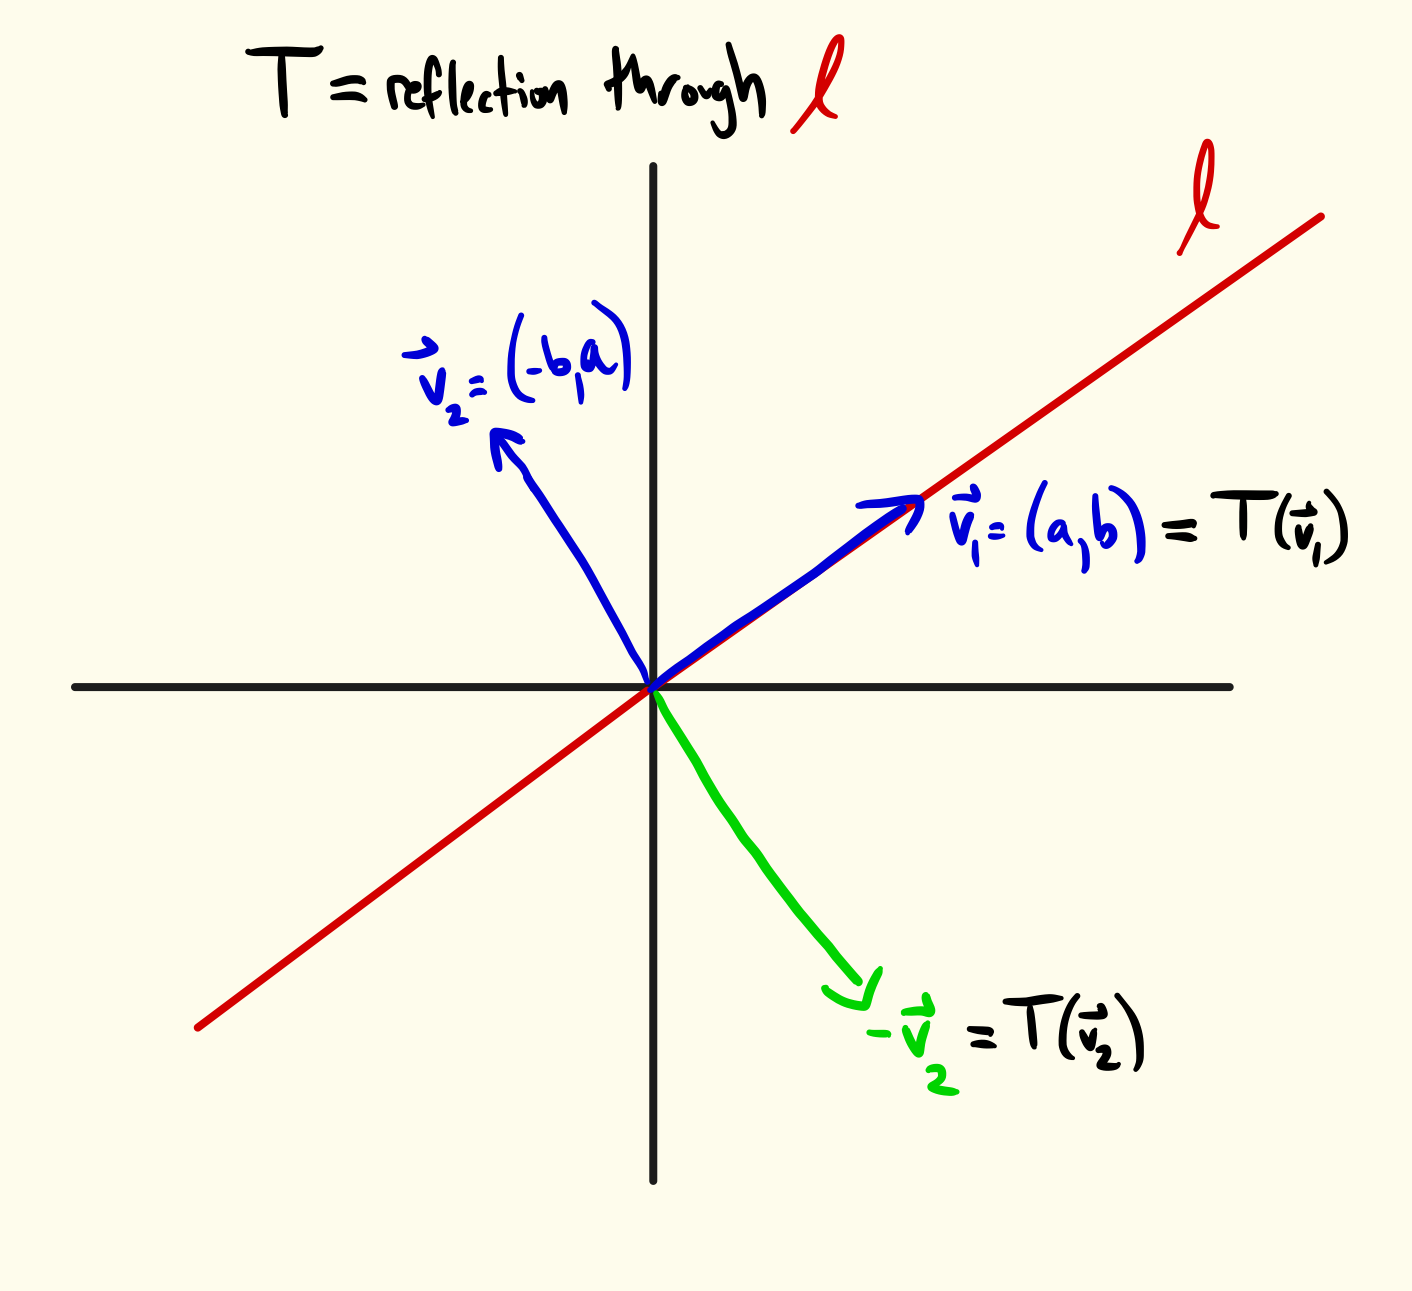
\includegraphics[width=4in]{../Lectures/Images/LineReflection}
\] 
Then we have 
\[
[T]_{B'}=\begin{bmatrix} \vert &\vert \\ [T(\boldv_1)]_{B'} & [T(\boldv_2)]_{B'}\\ \vert &\vert \end{bmatrix}=\begin{bmatrix} \vert &\vert \\ [\boldv_1]_{B'} & [-\boldv_2]_{B'}\\ \vert &\vert \end{bmatrix}=\begin{bmatrix}[rr]
1&0\\
0&-1
\end{bmatrix}.
\]
(b) To compute the $A$ such that $T=T_A$, note that $A=[T]_B$ where $B$ is the standard basis of $\R^2$. We can then use the change of basis formula: 
\[
A=[T]_B=\underset{B'\rightarrow B}{P}\ [T]_{B'}\ \underset{B\rightarrow B'}{P}
\]
We compute 
\[
\underset{B'\rightarrow B}{P}=\begin{bmatrix}
a&-b\\
b&a
\end{bmatrix}, \ \underset{B\rightarrow B'}{P}=\begin{bmatrix}
a&-b\\
b&a
\end{bmatrix}^{-1}=\frac{1}{a^2+b^2}\begin{bmatrix}
a&b\\
-b&a
\end{bmatrix}.
\]
Thus 
\[
A=[T]_B=\frac{1}{a^2+b^2}\begin{bmatrix}
a&-b\\
b&a
\end{bmatrix}\begin{bmatrix}
1&0\\
0&-1
\end{bmatrix}
\begin{bmatrix}
a&b\\
-b&a
\end{bmatrix}
=\frac{1}{a^2+b^2}\begin{bmatrix}
a^2-b^2&2ab\\
2ab&b^2-a^2
\end{bmatrix}.
\]
Recall that earlier we derived the formula 
\[
A=\begin{bmatrix}
\cos(2\theta) &\sin(2\theta)\\
\sin(2\theta)&-\cos(2\theta)
\end{bmatrix},
\]
where $\theta$ is the angle that the line $\ell$ makes with the $x$-axis. Is our new formula consistent with this? Observe that the vector $(a,b)$ has polar coordinates $(r,\theta)$ where 
\[
r=\sqrt{a^2+b^2}, \ \cos\theta=\frac{a}{\sqrt{a^2+b^2}},\  \sin\theta=\frac{b}{\sqrt{a^2+b^2}}.
\]
It follows that 
\[
\frac{1}{a^2+b^2}\begin{bmatrix}
a^2-b^2&2ab\\
2ab&b^2-a^2
\end{bmatrix}=
\begin{bmatrix}
\cos^2\theta-\sin^2\theta&2\cos\theta\sin\theta\\
2\cos\theta\sin\theta&\sin^2\theta-\cos^2\theta
\end{bmatrix}
=\begin{bmatrix}
\cos(2\theta) &\sin(2\theta)\\
\sin(2\theta)&-\cos(2\theta)
\end{bmatrix} \ \checkmark !
\]

\end{solution}
\ii {\em Reflection through the plane $\mathcal{P}\colon x+y+z=0$}. Define $T\colon \R^3\rightarrow \R^3$ to be reflection through the plane $\mathcal{P}\colon x+y+z=0$. See the next exercise for a precise definition of this operation. 
\bb
\ii Construct an explicit basis of the form $B'=\{\boldv_1,\boldv_2, (1,1,1)\}$ where $\boldv_1,\boldv_2$ are elements of $\mathcal{P}$. 
\ii Compute $[T]_{B'}$. 
\ii Find the $A$ such that $T=T_A$ using your result in (b) and a change of basis formula. 
\ii Compute $T(1,2,3)$. 
\ee
\begin{solution}
\noindent
This exercise is really just a special case of the next one. I give more details in the solution there. 
\\
(a) Set $B'=\{\boldv_1, \boldv_2, \boldn\}$, where $\boldv_1=(1,-1,0), \boldv_2=(0,1,-1), \boldn=(1,1,1)$. As is explained in more detail in the next exercise, we have $T(\boldv_1)=\boldv_1, T(\boldv_2)=\boldv_2$, and $T(\boldn)=-\boldn$. It follows that 
\[
[T]_{B'}=\begin{bmatrix}[rrr]
1&0&0\\
0&1&0\\
0&0&-1
\end{bmatrix}.
\]
(b) To compute $A=[T]_B$, we use the change of basis formula 
\begin{align*}
A=[T]_B&=\underset{B'\rightarrow B}{P}[T]_{B'}\underset{B\rightarrow B'}{P}\\
&=\begin{bmatrix}[rrr]
1&0&1\\
-1&1&1\\
0&-1&1
\end{bmatrix}
\begin{bmatrix}[rrr]
1&0&0\\
0&1&0\\
0&0&-1
\end{bmatrix}
\begin{bmatrix}[rrr]
1&0&1\\
-1&1&1\\
0&-1&1
\end{bmatrix}^{-1}\\
&=\frac{1}{3}
\begin{bmatrix}[rrr]
1&-2&-2\\
-2&1&-2\\
-2&-2&1
\end{bmatrix}.
\end{align*}
(c) We have 
\[
T(1,2,3)=A\begin{bmatrix}
1\\ 2\\ 3
\end{bmatrix}=\frac{1}{3}
\begin{bmatrix}[rrr]
1&-2&-2\\
-2&1&-2\\
-2&-2&1
\end{bmatrix}
\begin{bmatrix}
1\\ 2\\ 3
\end{bmatrix}
=\begin{bmatrix}[r]
-3\\ -2\\ -1
\end{bmatrix}
\]
\end{solution}

\ii {\em Reflection through a general plane in $\R^3$}. Fix $\boldn=(a,b,c)\ne \boldzero$. Let $W$ be the plane passing through the origin with normal vector $\boldn=(a,b,c)$: i.e., $W: ax+by+cz=0$. Reflection through $W$ is the map $T\colon\R^3\rightarrow\R^3$ defined as follows: 
\begin{quote}given $P=(x,y,z)$ let $\ell$ be the line passing through $P$ and perpendicular to $W$; let $Q$ be the intersection of this line with $W$; then the reflection $T(P)$ is the unique point $P'=(x',y',z')$ on $\ell$ such that the distance from $P$ to $P'$ is twice the distance from $P$ to $Q$. 
\end{quote}
Intuitively, $T(P)=P'$ is the point ``on the other side of the plane" from $P$ and an equal distance away. 
\\
You may take for granted that $T$ is a linear transformation. Also, observe that if $P$ lies in $W$, then the definition implies $T(P)=P$: $P$ is its own reflection. 
\\
Compute the matrix $A$ such that $T=T_A$ as follows: 
\bb
\ii First compute $A'=[T]_{B'}$, where $B'=\{\boldv_1,\boldv_2,\boldv_3\}$ is a basis for $\R^3$ satisfying $\boldv_1, \boldv_2\in W$, $\boldv_3=(a,b,c)$.
\ii Now use the change of basis formula to compute $A=[T]_B$, where $B$ is the standard basis. 
\ee
\begin{solution}
\noindent (a)  If we have a basis $B'$ as described, then $[T]_{B'}=\begin{bmatrix}
1&0&0\\
0&1&0\\
0&0&-1
\end{bmatrix}$. This is because $T$ fixes any vector in $W$ (reflection of point in plane is itself) and maps $\boldn$ to $-\boldn$. Once we have found the basis $B'$, letting $B$ be the standard basis, we have 
\[
A=[T]_B=\underset{B'\rightarrow B}{P}[T]_{B'}\underset{B\rightarrow B'}{P}.
\]
Furthermore, we know 
\[
\underset{B'\rightarrow B}{P}=\begin{bmatrix}
\vert&\vert&\vert\\
\boldv_1&\boldv_2&\boldv_3\\
\vert&\vert&\vert
\end{bmatrix}, \text{ and } \underset{B\rightarrow B'}{P}=(\underset{B'\rightarrow B}{P})^{-1}.
\]
So we are essentially done, except for some slightly unpleasant matrix arithmetic, after we find the basis $B'$. Let's do this now. 

To make our life easier, I assume that {\em at least two} of the elements $a, b, c$ are nonzero. The excluded case,  where exactly one of the elements $a$, $b$, and $c$ is nonzero,  would just be reflection through one of the coordinate planes, which is very easy to compute. Furthermore, the matrix formula we derive is valid even in these excluded cases, as you can check below! 

So assume that at least two of the elements $a,b,c$ are nonzero. Then $\boldv_1=(b,-a,0)$ and $\boldv_2=(0,c,-b)$ make up a basis of $W$, as is easily checked.  Setting $\boldv_3=\boldn$, we then have 
\[
\underset{B'\rightarrow B}{P}=\begin{bmatrix}
b&0&a\\
-a&c&b\\
0&-b&c
\end{bmatrix}
\]
and hence 
\begin{align*}
A&=\begin{bmatrix}
b&0&a\\
-a&c&b\\
0&-b&c
\end{bmatrix}
\begin{bmatrix}
1&0&0\\
0&1&0\\
0&0&-1
\end{bmatrix}
\left(\begin{bmatrix}
b&0&a\\
-a&c&b\\
0&-b&c
\end{bmatrix}
\right)^{-1}\\
&=\frac{1}{a^2+b^2+c^2}\begin{bmatrix}
-a^2+b^2+c^2&-2ab&-2ac\\
-2ab&a^2-b^2+c^2&-2bc\\
-2ac&-2bc&a^2+b^2-c^2
\end{bmatrix}
\end{align*}
Admittedly, I used technology to compute the inverse and the matrix multiplication in the last line. 
\end{solution}
%\ii {\em General rotation in $\R^3$}. Suppose $W$ is the plane passing through the origin perpendicular to a given {\em unit} normal vector $\boldn=(a,b,c)$: i.e., $W: ax+by+cz=0$ and $\norm{\boldn}=1$. Fix an angle $\theta$. We define $T$ to be rotation about $\boldn$ by $\theta$, where the positive rotational direction is taken to be counterclockwise with respect to $\boldn$. 
%\\
%In more detail: given $\boldv$, to compute $T(\boldv)$ you first write $\boldv=\boldw+\boldw^\perp$, where $\boldw=\proj{\boldv}{W}$ and $\boldw^\perp=\boldv-\boldw$ is the  component of $\boldv$ orthogonal to $W$.  Then define $T(\boldv)=\boldw'+\boldw^\perp$, where $\boldw'$ is the result of rotating $\boldw$ by $\theta$ in the plane $W$. 
%\\
%Thus $T$ rotates the projection of $\boldv$ onto $W$ by $\theta$ and leaves the orthogonal complement $\boldw^\perp$ untouched. Here is the picture:
%\[
%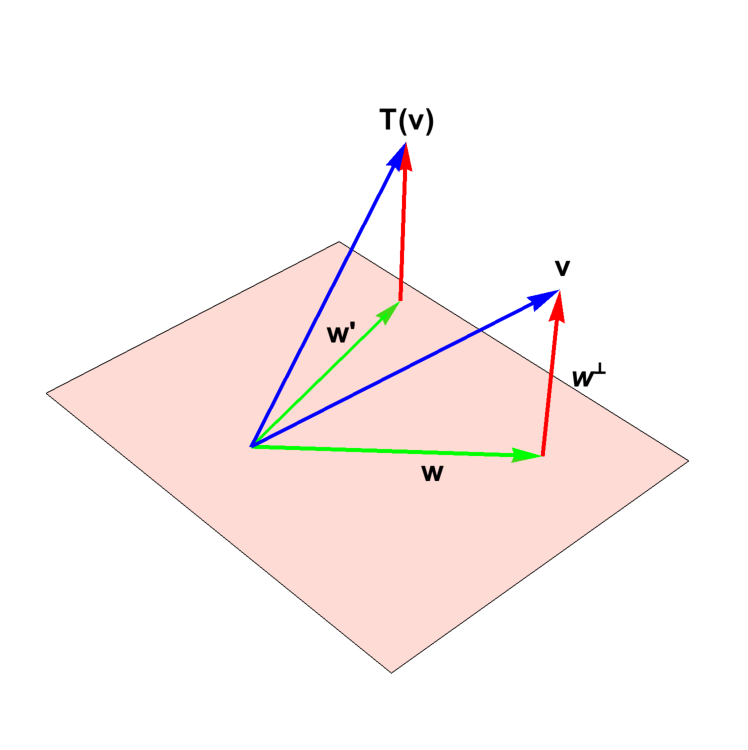
\includegraphics[width=2in]{GeneralRotation}
%\]
%Since rotation is an isometry that fixes the origin, $T$ is linear. As such we wish to come up with the matrix $A$ such that $T=T_A$. Below I outline two different methods. 
%\\
%(a) {\em Method 1}. Create a basis $B'$ of the form $\ds B'=\{ \boldw_1,\boldw_2,\boldn \}$, where $\boldw_1, \boldw_2$ are two orthonormal vectors in $W$. Compute $[T]_{B'}$ then convert everything to the standard basis $B$ using the change of basis formula for transformations. The basis $B'$ being orthonormal simplifies computations. 
%\\  
%(b) {\em Method 2}. (Requires the cross product) Given $\boldv=(x,y,z)$, describe $T(\boldv)$ in terms of the the three mutually orthogonal vectors  $\boldn$, $\boldw=\proj{\boldv}{W}$, and $\ds\boldw'=\boldn\times\proj{\boldv}{W}$. After some work you can derive the formula 
%\[
%T(\boldv)=\cos(\theta)\boldv+\sin(\theta)(\boldn\times\boldv)+((1-\cos \theta)\boldv\cdot\boldn)\boldn.
%\]
%Writing $\boldn=(a,b,c)$ and evaluating this formula for $T$ at $\boldv=(1,0,0), (0,1,0)$ and $(0,0,1)$ will give us the three columns of our matrix, expressed in terms of $a, b, c$ and $\theta$.  
%\\
%\begin{solution}
%%\ \\
%\noindent
%I'll let you think about this one some more. 
%\end{solution}
\ee

\setcounter{exercises@solutionnumber}{1}
\ \\
\section*{4.6: eigenvectors} \phantomsection \label{S:basissection}
\bb [itemsep=5pt]
\ii Compute the characteristic polynomial, eigenvalues, and eigenspace bases for each of the following matrices.
\bb[itemsep=5pt]
\ii
$A=
\begin{bmatrix}[cc]
2&1\\
1&2
\end{bmatrix}
$

\ii
$A=
\begin{bmatrix}[cc]
2&-3\\
0&2
\end{bmatrix}
$
\ii
$A=
\begin{bmatrix}[cc]
2&0\\
0&2
\end{bmatrix}
$
\ii 
$A=
\begin{bmatrix}[cc]
1&2\\
-2&-1
\end{bmatrix}
$
\ee
\begin{solution}
\noindent (a) 
The characteristic polynomial is
$$
\det(t I - A) =
\begin{vmatrix}[cc]
t - 2&-1\\
-1&t-2
\end{vmatrix}
= (t - 2)^2 - 1 = t^2 -4t +3 = (t - 3)(t - 1) =0
$$
Thus the eigenvalues are $\lambda = 3$ and $\lambda = 1$. 

For $W_3$ we see that $3I-A=
\begin{bmatrix}[rr]
1&-1\\
-1&1
\end{bmatrix}
$
has rank 1, and hence nullity 1. By inspection we see that $\boldv_1=(1,1)$ comprises a basis for $W_3$. 

For $\lambda = 1$, we have $I-A=
\begin{bmatrix}[rr]
-1&-1\\
-1&-1
\end{bmatrix}
$. Again, by inspection we see that $I-A$ has rank 1, hence nullity 1, and that $\boldv_2=(1,-1)$ forms a basis. 
\\
(b) 
$$
\det(t I- A) =
\begin{vmatrix}[cc]
t - 2& 3\\
0&t - 2
\end{vmatrix} =
t^2 - 4t + 4 = 0
$$
Which factors as $(t -2)^2 = 0$. Thus we have only one eigenvalue, $\lambda = 2$.

We have $2I-A=\begin{bmatrix}[cc]
0&3\\
0&0
\end{bmatrix}
$, a matrix of rank 1, and hence nullity 1. We see that $\boldv_1=(1,0)$ forms a basis for $W_2$. 
\\
(c) 
$$
\det(t I- A) =
\begin{vmatrix}[cc]
t - 2& 0\\
0&t - 2
\end{vmatrix} =
t^2 - 4t + 4 = 0
$$
Which factors as $(t -2)^2 = 0$. Thus we have only one eigenvalue, $t = 2$. 

We have $2I-A=\begin{bmatrix}[cc]
0&0\\
0&0
\end{bmatrix}
$
Then clearly $W_2=\NS(2I-A)=\R^2$, and $\{(1,0), (0,1)\}$ is a basis of $W_2$: i.e., all nonzero vectors of $\R^2$ are eigenvectors of $A$! 
 \\
(d) The characteristic polynomial is
$$
\det(t I- A) =
\begin{vmatrix}[cc]
t - 1& -\\
2&t + 1
\end{vmatrix} =
t^2 + 3 = 0
$$
Which does not have any real eigenvalues.
\end{solution}
\ii Compute the characteristic polynomial, eigenvalues, and eigenspace bases for
$$A=
\begin{bmatrix}[ccc]
1&0&-2\\
0&0&0\\
-2&0&4
\end{bmatrix}
$$
\begin{solution}
The characteristic polynomial is
$$
\det(t I - A) =
\begin{vmatrix}[ccc]
t - 1&0&2\\
0&t &0\\
2&0&t -4
\end{vmatrix}
=
t^3-5t = 0
$$
This factors as $t^2(t - 5)=0$. So the eigenvalues are $\lambda =0$ and $\lambda = 5$. To find the basis for $\lambda = 0$ we use
$$
\begin{bmatrix}[ccc]
-1&0&2\\
0&0&0\\
2&0&-4
\end{bmatrix}
\begin{bmatrix}[c]
x_1\\
x_2\\
x_3
\end{bmatrix}
=
\begin{bmatrix}[c]
0\\
0\\
0
\end{bmatrix}
$$
Thus $x_1 = 2x_3$, with the free variables $x_2=t$ and $x_3=r$.
$$
\begin{bmatrix}[c]
x_1\\
x_2\\
x_3
\end{bmatrix}
=
\begin{bmatrix}[c]
2r\\
t\\
r
\end{bmatrix}
=
r
\begin{bmatrix}[c]
2\\
0\\
1
\end{bmatrix} +t
\begin{bmatrix}[c]
0\\
1\\
0
\end{bmatrix}
$$
Thus the basis when $\lambda = 0$ is
$$
\left\{
\begin{bmatrix}[c]
2\\
0\\
1
\end{bmatrix},
\begin{bmatrix}[c]
0\\
1\\
0
\end{bmatrix}
\right\}
$$
Now for $\lambda = 5$ we use
$$
\begin{bmatrix}[ccc]
4&0&2\\
0&5&0\\
2&0&1
\end{bmatrix}
\begin{bmatrix}[c]
x_1\\
x_2\\
x_3
\end{bmatrix}
=
\begin{bmatrix}[c]
0\\
0\\
0
\end{bmatrix}
$$
Thus $x_1 = -1/2x_3$, $x_2 = 0$ and the free variable $x_3 = r$
$$
\begin{bmatrix}[c]
x_1\\
x_2\\
x_3
\end{bmatrix}
=
\begin{bmatrix}[c]
-1/2r\\
0\\
r
\end{bmatrix}
=
r
\begin{bmatrix}[c]
-1/2\\
0\\
1
\end{bmatrix}
$$
Thus the basis when $\lambda = 5$ is
$$
\left\{
\begin{bmatrix}[c]
-1/2\\
0\\
1
\end{bmatrix}
\right\}
$$
\end{solution}
\ii
Compute the characteristic polynomial, eigenvalues, and eigenspace bases for
$$A=
\begin{bmatrix}[ccc]
0&1&1\\
1&0&1\\
1&1&0
\end{bmatrix}
$$
\begin{solution}
The characteristic polynomial is
$$
\det(t I - A) =
\begin{vmatrix}[ccc]
t&-1&-1\\
-1&t &-1\\
-1&-1&t
\end{vmatrix}
=
t^3-3t - 2 = 0
$$
This factors as $(t+1)^2(t - 2)=0$. So the eigenvalues are $\lambda =-1$ and $\lambda = 2$. To find the basis for $\lambda = -1$ we use
$$
\begin{bmatrix}[ccc]
-1&-1&-1\\
-1&-1&-1\\
-1&-1&-1
\end{bmatrix}
\begin{bmatrix}[c]
x_1\\
x_2\\
x_3
\end{bmatrix}
=
\begin{bmatrix}[c]
0\\
0\\
0
\end{bmatrix}
$$
Thus $x_1 = -x_2-x_3$, with the free variables $x_2=t$ and $x_3=r$.
$$
\begin{bmatrix}[c]
x_1\\
x_2\\
x_3
\end{bmatrix}
=
\begin{bmatrix}[c]
-t-r\\
t\\
r
\end{bmatrix}
=
t
\begin{bmatrix}[c]
-1\\
1\\
0
\end{bmatrix} +r
\begin{bmatrix}[c]
-1\\
0\\
1
\end{bmatrix}
$$
Thus the basis when $\lambda = -1$ is
$$
\left\{
\begin{bmatrix}[c]
-1\\
1\\
0
\end{bmatrix},
\begin{bmatrix}[c]
-1\\
0\\
-1
\end{bmatrix}
\right\}
$$
Now for $\lambda = 2$ we use
$$
\begin{bmatrix}[ccc]
2&-1&-1\\
-1&2&-1\\
-1&-1&2
\end{bmatrix}
\begin{bmatrix}[c]
x_1\\
x_2\\
x_3
\end{bmatrix}
=
\begin{bmatrix}[c]
0\\
0\\
0
\end{bmatrix}
$$
Thus $x_1 = x_3$, $x_2 = x_3$ and the free variable $x_3 = r$
$$
\begin{bmatrix}[c]
x_1\\
x_2\\
x_3
\end{bmatrix}
=
\begin{bmatrix}[c]
r\\
r\\
r
\end{bmatrix}
=
r
\begin{bmatrix}[c]
1\\
0\\
1
\end{bmatrix}
$$
Thus the basis when $\lambda = 2$ is
$$
\left\{
\begin{bmatrix}[c]
1\\
1\\
1
\end{bmatrix}
\right\}
$$
\end{solution}
\ii 
Compute the characteristic polynomial, eigenvalues, and eigenspace bases for
$$A=
\begin{bmatrix}[ccc]
1&-3&3\\
3&-5&3\\
6&-6&4
\end{bmatrix}
$$
\begin{solution}
The characteristic polynomial is
$$
\det(t I - A) =
\begin{vmatrix}[ccc]
t-1&3&-3\\
-3&t + 5&-3\\
-6&6&t-4
\end{vmatrix}
=
t^3-12t - 16 = 0
$$
This factors as $(t+2)^2(t - 4)=0$. So the eigenvalues are $\lambda =-2$ and $\lambda = 4$. To find the basis for $\lambda = -2$ we use
$$
\begin{bmatrix}[ccc]
-3&3&-3\\
-3&3&-3\\
-6&6&-6
\end{bmatrix}
\begin{bmatrix}[c]
x_1\\
x_2\\
x_3
\end{bmatrix}
=
\begin{bmatrix}[c]
0\\
0\\
0
\end{bmatrix}
$$
Thus $x_1 = x_2-x_3$, with the free variables $x_2=t$ and $x_3=r$.
$$
\begin{bmatrix}[c]
x_1\\
x_2\\
x_3
\end{bmatrix}
=
\begin{bmatrix}[c]
t-r\\
t\\
r
\end{bmatrix}
=
t
\begin{bmatrix}[c]
1\\
1\\
0
\end{bmatrix} +r
\begin{bmatrix}[c]
-1\\
0\\
1
\end{bmatrix}
$$
Thus the basis when $\lambda = -2$ is
$$
\left\{
\begin{bmatrix}[c]
1\\
1\\
0
\end{bmatrix},
\begin{bmatrix}[c]
-1\\
0\\
1
\end{bmatrix}
\right\}
$$
Now for $\lambda = 4$ we use
$$
\begin{bmatrix}[ccc]
3&3&-3\\
-3&9&-3\\
-6&6&0
\end{bmatrix}
\begin{bmatrix}[c]
x_1\\
x_2\\
x_3
\end{bmatrix}
=
\begin{bmatrix}[c]
0\\
0\\
0
\end{bmatrix}
$$
Thus $x_1 = 1/2x_3$, $x_2 = 1/2x_3$ and the free variable $x_3 = r$
$$
\begin{bmatrix}[c]
x_1\\
x_2\\
x_3
\end{bmatrix}
=
\begin{bmatrix}[c]
1/2r\\
1/2r\\
r
\end{bmatrix}
=
r
\begin{bmatrix}[c]
1/2\\
1/2\\
1
\end{bmatrix}
$$
Thus the basis when $\lambda = 4$ is
$$
\left\{
\begin{bmatrix}[c]
1/2\\
1/2\\
1
\end{bmatrix}
\right\}
$$
\end{solution}

\ii Find the characteristic polynomial by inspection.
$$
\begin{bmatrix}[rrrr]
9&-8&6&3\\
0&-1&0&0\\
0&0&3&0\\
0&0&0&7
\end{bmatrix}
$$
\begin{solution}
Since the given matrix is upper triangular, so is $tI - A$. Since determinants of triangular matrices are just the product of their diagonal entries, we have 
\[
p(t)=\det(tI-A)=(t-9)(t+1)(t-3)(t-7).
\]
Similar reasoning shows, in general, that the eigenvalues of a triangular matrix (upper or lower or diagonal) are simply the entries along the diagonal. 
\end{solution}


\ii \label{ex:last} Let $A=\begin{bmatrix}[rrr] -5&0&3\\ -6&1&3\\ -6&0&4\end{bmatrix}$. 
Compute $p(t)$ and find bases for all eigenspaces of $A$. 
%\vfill
\\
\begin{solution}
	The characteristic polynomial of $A$ is $p(t)=t^3-3t+2=(t-1)^2(t+2)$. 
	
	We compute:
	\begin{align*}
	W_{1}&=\NS(I-A)=\Span(\{(1,0,2),(0,1,0) \})\\
	W_{-2}&=\NS(-2I-A)=\Span(\{(1,1,1)\})
	\end{align*}
\end{solution}
\ii The matrix $B=\begin{bmatrix}[rrr]-2&-3&3\\ -3&-3&4\\ -3&-4&5\end{bmatrix}$ has the same characteristic polynomial of $A$ in Exercise \ref{ex:last}. Find bases for all eigenspaces of $B$. 
%\vfill
\\
\begin{solution}
	Since $B$ also has characteristic polynomial $p(t)=(t-1)^2(t+2)$, it has only two eigenspaces. 
	
	We compute:
	\begin{align*}
	W_{1}&=\NS(I-B)=\Span(\{ (0,1,1) \})\\
	W_{-2}&=\NS(-2I-B)=\Span(\{(1,1,1)\})
	\end{align*}
	The two problems taken together show that the characteristic polynomial is not the whole story! The matrix $A$ has more linearly independent eigenvectors than $B$. 
\end{solution}
\ii Use induction to prove that if $\lambda$ is an eigenvalue of $A$, then $\lambda^k$ is an eigenvalue of $A^k$ for all positive integers $k$. Make sure to invoke the definition of eigenvalue in your proof. 
%\vfill
\begin{solution}
	Take $\boldv\ne \boldzero$ with $A\boldv=\lambda\boldv$. We show by induction that $A^k\boldv=\lambda^k\boldv$, and thus that $\lambda^k$ is an eigenvalue of $A^k$. 

The base case, $k=1$, is just the statement that $\boldv$ is an eigenvector. 

Induction step: assume $A^{k}\boldv=\lambda^k\boldv$. Then 
\begin{align*}
A^{k+1}\boldv &=AA^{k}\boldv\\
&=A(\lambda^k\boldv) &\text{(induction hypo.)}\\
&=\lambda^kA\boldv &\text{($\lambda$ is a scalar)}\\
&=\lambda^k\lambda\boldv&\text{($\boldv$ is an eigenvector)}\\
&=\lambda^{k+1}\boldv.
\end{align*} 
If we didn't know proof by induction, our ``proof" would look something like 
\begin{align*}
A^k\boldv &=\underbrace{A\cdot A\cdots A}_{\text{$k$ times}}\boldv\\
&=\underbrace{A\cdot A\cdots A}_{\text{$k-1$ times}}(A\boldv)\\
&=\underbrace{A\cdot A\cdots A}_{\text{$k-1$ times}}(\lambda\boldv) &\text{(since $A\boldv=\lambda\boldv$)}\\
&=\lambda\underbrace{A\cdot A\cdots A}_{\text{$k-1$ times}}(\boldv) &\text{(since $\lambda$ is a scalar)}\\
&=\lambda^2\underbrace{A\cdot A\cdots A}_{\text{$k-2$ times}}(\boldv) &\text{(by same logic)}\\
&\vdots \\
&=\lambda^{k-1}A\boldv \\
&=\lambda^k\boldv
\end{align*}
You can think of proof by induction as a way of replacing all these $\dots$ and $\ \vdots \ $ with a rigorous argument! 
\end{solution}
\ii Prove: $A$ is invertible if and only if $\lambda=0$ is {\em not} an eigenvalue of $A$. 
%\vfill
\\
\begin{solution}
There are many different ways of proving this.

Let $\lambda_1, \dots , \lambda_n$ be the eigenvalues of $A$. Recall that $\det(A)=\lambda_1\lambda_2\cdots \lambda_n$. 

Then we have 
\begin{align*}
A \text{ invertible} &\Leftrightarrow \det(A)\ne 0 \\
&\Leftrightarrow \lambda_1\lambda_2\cdots \lambda_n\ne 0\\
&\Leftrightarrow \lambda_i\ne 0 \text{ for all $i$}\\
&\Leftrightarrow 0 \text{ is not an eigenvalue of $A$}.
\end{align*}
\end{solution}
\ii
Let $B=\{\cos(x), \sin(x), \cosh(x), \sinh(x)\}$, let $V=\Span(B)$, and define $T\colon V\rightarrow V$ by $T(f)=f'$. 

You may take as a fact that the set $B$ is linearly independent, hence a basis. 

Recall: $\ds\cosh(x)=\frac{e^x+e^{-x}}{2}$, $\ds\sinh(x)=\frac{e^x-e^{-x}}{2}$. 
\bb
\ii Compute $A=[T]_B$. What does $A$ tell you about the invertibility of $T$?
\ii Find all eigenvalues of $T$.  
\ii For each eigenvalue $\lambda$ of $T$, find a basis for $W_\lambda$. 
\ii Use your work in (c) to find a new basis $B'$ of $V$ that contains two eigenvectors of $T$.
\ii  Compute $[T]_{B'}$. 
\ee
%\vfill
\begin{solution}
	We find that $A=\begin{bmatrix}
	0&1&0&0\\
	-1&0&0&0\\
	0&0&0&1\\
	0&0&1&0
	\end{bmatrix}$.
	\\
	Since $A$ is invertible (its rank is clearly 4), it follows that $T$ is invertible. 
	\\ \\
	The characteristic polynomial of $A$ (in factored form) is $p(t)=(t-1)(t+1)(t^2+1)$. Thus the eigenvalues of $A$ (and hence also $T$) are $\lambda=1$ and $\lambda=-1$. 
	
	We compute bases for the eigenspaces of $A$:
	\begin{align*}
	W_1&=\NS(I-A)=\Span(\{ (0,0,1,1)\}\\
	W_{-1}&=\NS(-I-A)=\Span(\{(0,0,1,-1)\}
	\end{align*}
	Lifting these vectors back to $V$ via the $[\hspace{5pt}]_B$ map yields bases for the same eigenspaces of $T$: \begin{align*}
	W_1&=\Span(\{\cosh x+\sinh x\}=\Span(\{e^x\})\\
	W_{-1}&=\Span(\{\cosh x-\sinh x\}=\Span(\{e^{-x}\})
	\end{align*}
	We construct the new basis $B'=\{\cos(x),\sin(x),e^x, e^{-x}\}$ (it is easy to see that these four functions are independent), and compute 
	\[
	A'=[T]_{B'}=\begin{bmatrix}
	0&1&0&0\\
	-1&0&0&0\\
	0&0&1&0\\
	0&0&0&-1
	\end{bmatrix}
	\]
\end{solution}
\ii Suppose $A$ is a $2\times 2$ matrix satisfying $\tr A=2$ and $\det A=-15$. Find the eigenvalues of $A$.
\\
\begin{solution}
Let $\lambda, \lambda'$ be the eigenvalues of $A$ (possibly complex, possibly repeated). We have 
\begin{align*}
\lambda+\lambda'&=\tr A=2 &\text{(trace is the sum of the eigenvalues)}\\
\lambda\lambda'&=\det A=-15&\text{(det. is the product of the eigenvalues)}
\end{align*}
The system implies $\lambda'=2-\lambda$, and hence that $\lambda^2-2\lambda-15=0$. Thus $\lambda=5$ or $\lambda=-3$. Thus the eigenvalues of $A$ are $5$ and $-3$. 

Alternatively, the characteristic polynomial of $A$ is 
\[
p(x)=x^2-\tr A x+\det A=x^2-2x-15=(x-5)(x+3).
\]
Thus the eigenvalues of $A$ are $5$ and $-3$. 

\end{solution} 
\ii Let $T\colon V\rightarrow V$ be a linear transformation, and suppose $B=\{\boldv_1, \boldv_2,\dots, \boldv_n\}$. 

\noindent
Prove: $[T]_B$ is a diagonal matrix if and only if $\boldv_j$ is an eigenvector of $T$ for all $1\leq i\leq n$. 

\noindent
{\em Moral}. We can represent $T$ by a diagonal matrix if and only if $T$ has ``enough" linearly independent eigenvectors to build a basis. 
\\
\begin{solution}
\noindent
We prove the two implications separately. 
\vspace{.1in}
\\
($\Rightarrow$) Suppose the vectors $\boldv_i$ are all eigenvectors with $T(\boldv_i)=\lambda_i\boldv_i$. Using the recipe for $[T]_{B}$ we compute 
\begin{align*}
[T]_B&=\begin{bmatrix}
\vert &\vert & &\vert\\
[T(\boldv_1)]_B&[T(\boldv_2)]&\cdots &[T(\boldv_n)]_B\\
\vert &\vert & &\vert
\end{bmatrix}\\
&=\begin{bmatrix}
\vert &\vert & &\vert\\
[\lambda_1\boldv_1]_B&[\lambda_2\boldv_2]&\cdots& [\lambda_n\boldv_n]_B\\
\vert &\vert & &\vert
\end{bmatrix}\\
&=\begin{bmatrix}\lambda_1&0&\cdots &0\\
0&\lambda_2&\cdots&0\\
\vdots & & &\\
0&0&\cdots&\lambda_n
\end{bmatrix},
\end{align*}
where the last equality holds since $\lambda_1\boldv_1=\lambda_1\boldv_1+0\boldv_2+\dots, \lambda_2\boldv_2=0\boldv_1+\lambda_2\boldv_2+0\boldv_3+\dots$, etc. 
\vspace{.1in}
\\
($\Leftarrow$) Suppose 
\[
[T]_B=D=\begin{bmatrix}d_1&0&\cdots &0\\
0&d_2&\cdots&0\\
\vdots & & &\\
0&0&\cdots&d_n
\end{bmatrix}.
\]
I claim $T(\boldv_i)=d_i\boldv_i$ for all $i$, which proves $B$ consists of eigenvectors of $T$. To do so, first observe that 
\begin{align*}
[T(\boldv_i)]_B&=[T]_B[\boldv_i]_B &\text{(defining property of $[T]_B$)}\\
&=D\bolde_i &\text{(since $[\boldv_i]_B=(0,0,\dots, 1,0,\dots, 0)=\bolde_i$)}\\
&=\begin{bmatrix}
0\\ \vdots \\ d_i\\ \vdots \\ 0
\end{bmatrix}.
\end{align*}
But we have $[T(\boldv_i)]_B=(0,0,\dots, d_i, 0,\dots, 0)$ if and only if $T(\boldv_i)=d_i\boldv_i$, by definition of the coordinate vector map. This proves each $\boldv_i$ is an eigenvector with eigenvalue $d_i$. 
\end{solution}
\ee


	\setcounter{exercises@solutionnumber}{1}
\ \\
\section*{4.7: diagonalization} \phantomsection \label{S:basissection}
\bb[itemsep=5pt, topsep=5pt]

\ii Find the eigenvalues of $A$. For each eigenvalue $\lambda$, find the rank of the matrix $\lambda I - A$. Is $A$ diagonalizable? Justify.
\[
A=
\begin{bmatrix}[rrr]
3&0&0\\
0&2&0\\
0&1&2
\end{bmatrix}
\]
\\
\begin{solution}
\noindent We compute $p(t)$: 
$$
\det(t I - A) =
\begin{vmatrix}[rrr]
t - 3&0&0\\
0&t - 2&0\\
0&-1&t - 2
\end{vmatrix}
= (t - 3)(t - 2)^2 = 0
$$
Thus the eigenvalues are $\lambda =3$ and $\lambda = 2$.
\\
We compute $\dim W_3=\NS(3I-A)$: 
\[
3I-A=
\begin{bmatrix}[rrr]
0&0&0\\
0&1&0\\
0&-1&1
\end{bmatrix}
\]
Since the rank of this matrix is 2, its nullity is 3-2=1. This means $\dim(W_{3})=1$. 
\\
Next, we have 
$$2I-A=
\begin{bmatrix}[rrr]
-1&0&0\\
0&0&0\\
0&-1&0
\end{bmatrix}
$$
Once again the nullity is 1, which means $\dim(W_2)=1$. Since the sum of the dimensions of the eigenspaces is $1+1\ne 3$, we conclude that $A$ is not diagonalizable. 
\end{solution}

\ii  For each matrix $A$ below, find the geometric and algebraic multiplicity of each eigenvalue of the matrix $A$, and determine whether $A$ is diagonalizable. If $A$ is diagonalizable, then find the matrix $P$ that diagonalizes $A$, and find $P^{-1}AP$.
\bb[itemsep=5pt, topsep=5pt]
\ii 
\[
A =
\begin{bmatrix}[rrr]
-1&4&-2\\
-3&4&0\\
-3&1&3
\end{bmatrix}
\]
\ii 
\[
A=
\begin{bmatrix}[ccc]
19&-9&-6\\
25&-11&-9\\
17&-9&-4
\end{bmatrix}
\]
\ii 
\[
A=
\begin{bmatrix}[rrr]
0&0&0\\
0&0&0\\
3&0&1
\end{bmatrix}
\]
\ii
\[
A =
\begin{bmatrix}[rrr]
5&0&0\\
1&5&0\\
0&1&5
\end{bmatrix}
\]
\ee
\begin{solution}
\noindent 
(a) Start by finding the eigenvalues of matrix $A$.
$$
\det(t I - A) =
\begin{vmatrix}[rrr]
t +1&-4&2\\
3&t - 4&0\\
3&-1&t - 3
\end{vmatrix}
= (t - 1)(t - 2)(t - 3) = 0
$$
We have a theorem that says a matrix $A\in M_{nn}$ with $n$ distinct eigenvalues is diagonalizable. Thus $A$ is diagonalizable. To construct the matrix $P$, we need to come up with bases for each space $W_\lambda=\NS(\lambda I-A)$. Each of these has dimension 1, and we easily come up with bases by inspection. This yields the basis $\boldv_1=(1,1,1)$, $\boldv_2=(2,3,3)$ and $\boldv_3=(1,3,4)$.  

According to the recipe, we then have 
$$
P =
\begin{bmatrix}[ccc]
1&2&1\\
1&3&3\\
1&3&4
\end{bmatrix}
,  D=
\begin{bmatrix}[rrr]
1&0&0\\
0&2&0\\
0&0&3
\end{bmatrix}, \text{ and } D=P^{-1}AP.
$$
\\
(b) 
Start by finding the eigenvectors in the usual way
$$\det(t I - A) =
\begin{vmatrix}[ccc]
t-19 &9&6\\
-25&t+11&9\\
-17&9&t +4
\end{vmatrix}
= t^3 - 4t^2+5t-2 = (t -1)^2(t-2) = 0
$$
For $\lambda = 1$, we can see that the algebraic multiplicity is 2. Consider the matrix
$$
\begin{bmatrix}[ccc]
-18 &9&6\\
-25&12&9\\
-17&9&5
\end{bmatrix}
\rightarrow
\begin{bmatrix}[ccc]
1&0&-1\\
0&1&-4/3\\
0&0&0
\end{bmatrix}
$$
Thus the rank is 2 and the geometric multiplicity is 1. Since the geometric multiplicity is less than the algebraic multiplicity for one of the eigenspaces, we know immediately that $A$ is not diagonalizable. 

However, we continue on nonetheless. For $\lambda =2$, we can see that the algebraic multiplicity is 1. We know that $1\leq \dim W_2\leq 1$, hence we must have $\dim W_2=1$. Let's verify this: 
$$
2I-A=
\begin{bmatrix}[ccc]
-17 &9&6\\
-25&13&9\\
-17&9&6
\end{bmatrix}
\rightarrow
\begin{bmatrix}[ccc]
1&0&-3/4\\
0&1&-3/4\\
0&0&0
\end{bmatrix},
$$
a matrix of rank 2, and hence nullity 1. 

Lastly, we see that $\dim W_1+\dim W_2=1+1=2\ne 3$. Hence $A$ is not diagonalizable, as we claimed above. 
\\
(c)
$$\det(t I - A) =
\begin{vmatrix}[ccc]
t &0&0\\
0&t&0\\
-3&0&t -1
\end{vmatrix}
= t^2(t -1) = 0
$$
Thus the eigenvalues are $\lambda =0$ and $\lambda = 1$. For $\lambda =0$, notice that the algebraic multiplicity is 2. Now consider the matrix
$$
\begin{bmatrix}[rrr]
0&0&0\\
0&0&0\\
-3&0&-1
\end{bmatrix}
$$
The rank is 1, thus the geometric multiplicity is  2.  For $\lambda = 1$, notice that the algebraic multiplicity is 1. Now consider the matrix
$$
\begin{bmatrix}[rrr]
1&0&0\\
0&1&0\\
-3&0&0
\end{bmatrix}
$$
The rank is 2, thus the geometric multiplicity is 1. Since for all $\lambda$ the geometric multiplicity is equal to the algebraic multiplicity, the initial matrix is diagonalizable.  As usual, we build $P$ by first computing bases for $W_0$ and $W_1$, and then putting these in as the columns of $P$. One possible answer is 
$$P =
\begin{bmatrix}[ccc]
-1&0&0\\
0&1&0\\
3&0&1
\end{bmatrix}
$$
with corresponding 
\[
D=
\begin{bmatrix}[rrr]
0&0&0\\
0&0&0\\
0&0&1
\end{bmatrix}
\]
\ \\
(d)
$$\det(t I - A) =
\begin{vmatrix}[ccc]
t - 5&0&0\\
-1&t-5&0\\
0&-1&t -5
\end{vmatrix}
= (t -5)^3 = 0
$$
Thus $\lambda = 5$ is the only eigenvalue and its algebraic multiplicity is 3. Now considering when $\lambda$ is 5, we look at the matrix
$$
\begin{bmatrix}[rrr]
0&0&0\\
-1&0&0\\
0&-1&0
\end{bmatrix}
$$
The rank of this matrix is 2, thus the geometric multiplicity is 1. Since algebraic multiplicity is not equal to the geometric multiplicity, the initial matrix is not diagonalizable.
\end{solution}
\ii Let $A=\begin{bmatrix}
a&b\\ c&d
\end{bmatrix}$. Derive necessary and sufficient conditions for $A$ to be diagonalizable expressed in terms of equalities and inequalities involving $a,b,c,d$. 
\\
\begin{solution}
\noindent
First analyze the diagonalizability of $A$ based on the number of distinct real eigenvalues it has: 0, 1, or 2. 

\noindent
If $A$ has 0 eigenvalues, then it is clearly not diagonalizable, as it has no eigenvectors. 

\noindent
If $A$ has 2 distinct eigenvalues, then it is automatically diagonalizable, by the corollary to the linear independence of eigenvectors theorem. 

\noindent
If $A$ has exactly one eigenvalue $\lambda$, then $A$ is diagonalizable if and only if $\dim W_\lambda =2$ (by the diagonalization theorem) if and only if $\dim\NS \lambda I -A=2$ if and only if $\rank \lambda I-A=0$ if and only if $\lambda I-A=\underset{2\times 2}{\boldzero}$ if and only if $A=\lambda I$ is diagonal !!

\noindent
We conclude that $A$ is diagonalizable if and only if (a) it has two distinct eigenvalues or (b) it has one eigenvalue and is diagonal. We can relate these conditions to $a,b,c,d$ by looking at the characteristic polynomial $p(x)$. 

\noindent
The characteristic polynomial of $A=\begin{bmatrix}
a&b\\ c&d
\end{bmatrix}$ is $p(x)=x^2-(a+d)x+(ad-bc)$. Its roots are given by 
\[
x=\frac{1}{2}(a+d\pm \sqrt{a^2+2ad+d^2-4ad+4bc}\ )=\frac{1}{2}(a+d\pm \sqrt{(a-d)^2+4bc}\ )
\]
We see that (a) $A$ has two real eigenvalues iff $(a-d)^2>-4bc$, and that (b) $A$ is diagonal with one distinct eigenvalue iff $a=d$ and $b=c=0$. 

\noindent
We conclude: 
\[
\text{$A$ is diagonalizable } \Longleftrightarrow (a-d)^2>-4bc\text{ or } a-d=b=c=0.
\]
\end{solution}
\ii Prove all statements of the properties of similarity theorem, stated below. 
\begin{namedtheorem}[Properties of similarity theorem]
 Suppose $A$ is similar to $B$: i.e., there is an invertible matrix $P$ such that $B=P^{-1}AP$. Then:
 \bb[(a)]
\ii $B$ is similar to $A$. ({\em Similarity is symmetric}.)
\ii $A$ and $B$ have the same trace and determinant. 
\ii $A$ and $B$ have the same rank nullity and rank. 
\ii $A$ and $B$ have the same characteristic polynomial.  
\ii $A$ and $B$ have the same eigenvalues. 
\ii Given any $\lambda\in\R$, let $W_\lambda$ be the corresponding eigenspace for $A$, and $W_\lambda'$ the corresponding eigenspace for $B$. Then $\dim W_{\lambda}=\dim W_{\lambda}'$. 
\ee
 \end{namedtheorem}
\begin{solution}
\noindent
(a) If $B=P^{-1}AP$, then $A=PBP^{-1}=Q^{-1}BQ$, where $Q=P^{-1}$. 
\vspace{.1in}
\\
(d) This was proven in the lecture notes. 
\vspace{.1in}
\\
(b)\& (e) Follow directly from (d) and our theorem about characteristic polynomials. Indeed, let $p(x)=x^n+a_{n-1}x^{n-1}+\cdots +a_1x+a_0$ be the characteristic polynomial of $A$ and $B$. Then $\tr A=\tr B=-a_{n-1}$, $\det A=\det B=(-1)^na_0$, and the eigenvalues of both $A$ and $B$ are precisely the roots of $p(x)$. 
(c) I claim $\boldx'\in \NS B$ if and only if $\boldx'=P^{-1}\boldx$ for some $\boldx\in \NS B$. To see this, first observe that if $\boldx\in\NS A$, then 
\[
B\boldx'=B(P^{-1}\boldx)=P^{-1}AP(P^{-1}\boldx)=P^{-1}A\boldx=\boldzero.
\]
Now suppose $\boldx'\in \NS B$. A similar argument (using $A=PBP^{-1}$) shows that $\boldx=P\boldx'\in \NS A$; and we have $\boldx'=P\boldx$.
\vspace{.1in}
\\
From our claim it follows that $P^{-1}$ defines an invertible linear transformation (with inverse $P$) from $\NS A$ to $\NS B$. In fancy terms this means $\NS A$ and $\NS B$ are isomorphic, and hence have the same dimension. More directly, if $B=\{\boldv_1,\dots, \boldv_r\}$ is a basis for $\NS A$, then you can show that $\{P^{-1}\boldv_1, P^{-1}\boldv_2, \dots , P^{-1}\boldv_r\}$ is a basis for $\NS B$.  
\vspace{.1in}
\\
Either way, we see that $\nullity A=\dim \NS A=\dim\NS B=\nullity B$. The rank-nullity theorem then implies that $\rank A=\rank B$. 
\vspace{.1in}
\\
(f) An argument exactly like the the one above shows that the map $\boldx\mapsto P^{-1}\boldx$ defines an invertible linear transformation from $W_\lambda$ to $W_\lambda'$, and that $P^{-1}$ maps any basis of $W_{\lambda}$ to a basis of $W_{\lambda}'$. Thus $\dim W_{\lambda}=\dim W_{\lambda}'$. 
\end{solution}
\ii Similar matrices have the same rank. Show the converse is false by showing the matrices
$$
A =
\begin{bmatrix}[rr]
1&0\\
0&0
\end{bmatrix}
,
B =
\begin{bmatrix}[rr]
0&1\\
0&0
\end{bmatrix}
$$
have the same rank, but are not similar.
\\
\begin{solution}Notice that $\rank(A) = \rank(B) = 1$. Also notice that $\tr(A) = 1 \neq 0 = \tr(B)$. Since the traces are different, the matrices are not similar. 
\end{solution}
\ii Similar matrices have the same eigenvalues. Show the converse is false by showing the matrices
$$
A =
\begin{bmatrix}[rr]
1&1\\
0&1
\end{bmatrix}
,
B =
\begin{bmatrix}[rr]
1&0\\
0&1
\end{bmatrix}
$$
have the same eigenvalues, but are not similar.
\\
\begin{solution}
Notice both $A$ and $B$ are triangular, thus $\det(t I - A) = (t - 1)^2 = \det(t I -B)$. Thus $\lambda = 1$ is the only eigenvalue for both $A$ and $B$. 

However, as one can easily compute, for $A$ the eigenspace $W_1$ has dimension 1, whereas for $B$ the eigenspace $W_1$ has dimension 2. Thus the two cannot be similar! 
\end{solution}
\ii Prove that if $B = P^{-1}AP$, and $\boldv$ is an eigenvector of $B$ corresponding to the eigenvalue $\lambda$, the $P\boldv$ is the eigenvector of $A$ corresponding to $\lambda$.
\\
\begin{solution}
We assume that $\boldv$ is an eigenvector of $B$, and must show that $P\boldv$ is an eigenvector of $A$. 

Thus by definition of eigenvector we assume
\bb[(i)]
\ii $B\boldv=\lambda\bold v$, and 
\ii $\boldv\ne\boldzero$. 
\ee
But then 
\begin{align*}
A(P\boldv)&=AP\boldv\\
&=PB\boldv &\text{(since $B=P^{-1}AP$)}\\
&=P(\lambda\boldv) &\text{ (since $B\boldv=\lambda\boldv$)}\\
&=\lambda P\boldv) &\text{ (since $\lambda$ is a scalar)}.
\end{align*}
Thus $A(P\boldv)=\lambda P(\boldv)$. 

To show $P\boldv$ is an eigenvector, it remains only to show that $P\boldv\ne\boldzero$. But since $P$ is invertible, and since $\boldv\ne\boldzero$, it follows that $P\boldv\ne\boldzero$. 
\end{solution}
\ii \label{ex:conjpoly}
Let $A$ be an $n$ by $n$ matrix, and let $q(A)$ be the matrix
$$
q(A) = a_nA^n +a_{n-1}A^{n-1}+\cdots+a_1A+a_0I_n
$$
Prove that if $B = P^{-1}AP$, then $q(B) = P^{-1}q(A)P$.
\\
\begin{solution}
First we need to show (by induction) that $B^n =P^{-1}A^nP$ for all $n$. The base case, when $n=1$ is give by the hypothesis. Assume that equality holds when $n \leq k$. We need to show that equality holds when $n = k+1$.
\begin{eqnarray*}
B^{k+1} &=& BB^k\\
&=&(P^{-1}AP)B^k\\
&=& (P^{-1}AP)(P^{-1}A^kP)\\
&=& P^{-1}A(PP^{-1})A^kP\\
&=&P^{-1}A^{k+1}P
\end{eqnarray*}
Thus $B^n =P^{-1}A^nP$ holds for all $n$. Now we can show the desired result.
\begin{eqnarray*}
q(B) &=& a_nB^n + a_{n-1}B^{n-1}+\cdots+a_1B+a_0I_n\\
&=& a_n(P^{-1}A^nP) + a_{n-1}(P^{-1}A^{n-1}P)+\cdots+a_1(P^{-1}AP)+a_0I_n\\
&=& P^{-1}(a_nA^nP) + (a_{n-1}A^{n-1}P)+\cdots+(a_1AP)+a_0I_n)\\
&=&P^{-1}(a_nA^n) + (a_{n-1}A^{n-1})+\cdots+(a_1A)+a_0I_n)P\\
&=& P^{-1}(q(A))P
\end{eqnarray*}
\end{solution}

\ii  Let $A$ be a $3\times 3$ matrix with eigenvalues $1, -1, 0$. 
\bb
\ii Prove that $A$ is diagonalizable. What is $D$ in this case?
\ii Show that $A^n=A$ for any {\bf odd} $n\geq 0$: e.g., $A^{13}=A$, $A^{77}=A$, etc.
\ee
\begin{solution}
%\ \\
The matrix is diagonalizable as it has three distinct eigenvalues. We have $D=P^{-1}AP$ where $D=\begin{bmatrix}
1&0&0\\
0&-1&0\\
0&0&0
\end{bmatrix}$. 
\\
It is easy to see that 
\[
D^n=\begin{bmatrix}
1^n&0&0\\
0&(-1)^n&0\\
0&0&0^n
\end{bmatrix}
=\begin{bmatrix}
1&0&0\\
0&(-1)^n&0\\
0&0&0
\end{bmatrix}
\]
Thus we see clearly that $D^n=D$ if and only if $n$ is odd. 

Next, write $A=PDP^{-1}$. Then $A^n=(PDP^{-1})^n=PD^nP^{-1}$, where this last step is the extremely useful fact that ``conjugation respects powers of matrices".  If $n$ is odd, we thus have $A^n=PD^nP^{-1}=PDP^{-1}=A$, as claimed. 
\end{solution}
\ii The {\em Fibonacci sequence} $F_0, F_1, F_2, \dots$ is defined recursively as follows: 
\begin{align*}
F_0&=0\\
F_1&=1\\
F_n&=F_{n-2}+F_{n-1} &\text{for $n\geq 2$}
\end{align*}
Let $A=\begin{bmatrix}
0&1\\
1&1
\end{bmatrix}$.
\bb
\ii Show that 
\[
A^n\begin{bmatrix}
0 \\ 1
\end{bmatrix}=\begin{bmatrix}
F_n\\ F_{n+1}
\end{bmatrix}
\]
for all $n\geq 0$. 
\ii Diagonalize $A$. Write its two eigenvalues as $\lambda_1$ and $\lambda_2$. 

\ii Derive a closed formula for $A^n$. 

\ii Derive  a closed formula for $F_n$. 

\ee
\begin{solution}
\noindent
(a) Proof by induction. Base case ($n=0$) is trivial. For induction step, suppose 
$A^n\begin{bmatrix}
0 \\ 1
\end{bmatrix}=\begin{bmatrix}
F_n\\ F_{n+1}
\end{bmatrix}$, then 
\begin{align*}
A^{n+1}\begin{bmatrix}
0\\ 1
\end{bmatrix}&=AA^n\begin{bmatrix}
0\\ 1
\end{bmatrix}\\
&=A\begin{bmatrix}
F_n\\ F_{n+1}
\end{bmatrix} &\text{(induction hypo.)}\\
&=\begin{bmatrix}
F_{n+1}\\ F_n+F_{n+1}
\end{bmatrix}\\
&=\begin{bmatrix}
F_{n+1}\\ F_{n+2}.
\end{bmatrix}
\end{align*}
as desired. 
\vspace{.1in}
\\
(b) The eigenvalues of $A$ are $\lambda_1=\frac{1}{2}(1+\sqrt{5})$ and $\lambda_2=\frac{1}{2}(1-\sqrt{5})$.
\\
Note that the $\lambda_i$ satisfy\\
$\lambda_1+\lambda_2=1$\\
$\lambda_1\lambda_2=-1$\\
$\lambda_1^2=\lambda_1+1$, $\lambda_2^2+\lambda_2=1$. 
\\
(These follow from the fact that they are roots of $p(x)=x^2-x-1=(x-\lambda_1)(x-\lambda_2)$. )
\vspace{.1in}
\\
From these relations it is easy to verify that 
$\boldv_1=(1,\lambda_1)$ and $\boldv_2=(1,\lambda_2)$ form bases of $W_{\lambda_1}$ and $W_{\lambda_2}$, respectively. 
\vspace{.1in}
\\
Then we have $D=P^{-1}AP$ where 
\[
D=\begin{bmatrix}[rr]
\lambda_1&0\\
0&\lambda_2
\end{bmatrix}, \ P=\begin{bmatrix}[rrr]
1&1\\
\lambda_1&\lambda_2
\end{bmatrix}, \ P^{-1}=-\frac{1}{\sqrt{5}}\begin{bmatrix}[rrr]
\lambda_2&-1\\
-\lambda_1&1
\end{bmatrix}.
\]
(c) 
Now we compute  
\[
A^n=(PDP^{-1})^n=PD^nP^{-1}=-\frac{1}{\sqrt{5}}\begin{bmatrix}[rrr]
1&1\\
\lambda_1&\lambda_2
\end{bmatrix}\begin{bmatrix}[rr]
\lambda_1^n&0\\
0&\lambda_2^n
\end{bmatrix}\begin{bmatrix}[rrr]
\lambda_2&-1\\
-\lambda_1&1
\end{bmatrix}
=\frac{1}{\sqrt{5}}\begin{bmatrix}
\lambda_1^{n-1}-\lambda_2^{n-1}&\lambda_1^n-\lambda_2^n\\
\lambda_1^n-\lambda_2^n&\lambda_1^{n+1}-\lambda_2^{n+1}
\end{bmatrix}
\]
(d) Lastly, using our formula above for $A^n$ we see that
\[
\begin{bmatrix}
F_n\\
F_{n+1}
\end{bmatrix}=A^n\begin{bmatrix}
0\\1
\end{bmatrix}
=\frac{1}{\sqrt{5}}\begin{bmatrix}
\lambda_1^n-\lambda_2^n\\
\lambda_1^{n+1}-\lambda_2^{n+1}
\end{bmatrix}.
\]
It follows that 
\[
F_n=\frac{1}{\sqrt{5}}(\lambda_1^{n}-\lambda_2^n), 
\]
where $\lambda_1=\frac{1}{2}(1+\sqrt{5}), \lambda_2=\frac{1}{2}(1-\sqrt{5})$. 
\end{solution}
\ii Let $A\in M_{nn}$ be defined as the matrix of all 1's: i.e., $a_{ij}=1$ for all $1\leq i, j\leq n$. 
\\
Show that $A$ has exactly 2 eigenvalues and that $A$ is diagonalizable. 
\\
Hint: do NOT compute the characteristic polynomial of $A$. Instead, begin by first considering $\NS(A)$. 
\\
\begin{solution}
%\ \\
\noindent 
Since $\rank(A)=1$, we have $\nullity(A)=\dim W_0=n-1$. Thus $0$ is an eigenvalue of $A$ with geometric multiplicity $n-1$. Since geometric multiplicity is bounded by algebraic multiplicity, we must have the characteristic polynomial $p(t)$ factoring as $p(t)=t^{n-1}(t-c)$ for some $c\in \R$. (Remember that $\deg p(t)=n$.) Now use the fact that 
\[
n=\tr A=(\text{sum of eigenvalues})=0+0+\cdots +0+c.
\]
It follows that $c=n$. Thus the distinct eigenvalues of $A$ are $0$ and $c$. Since $\dim W_0=n-1$ and $1\leq \dim W_n\leq 1$, we have 
\[
\dim W_0+\dim W_n=n-1+1=n.
\] 
Thus $A$ is diagonalizable. 

By the way, try diagonalizing $A$ yourself: that is, produce a basis of eigenvectors. 
\end{solution}
\ii The {\em Cayley-Hamilton theorem} states that any $A\in M_{nn}$ satisfies its own characteristic polynomial $p(t)$: i.e., $p(A)=\boldzero_{n\times n}$. 

Prove the Cayley-Hamilton theorem for {\em diagonalizable} matrices. 
\\
\begin{solution}
%\ \\
\noindent 
First, since $A$ is diagonalizable, we write $D=P^{-1}AP$ where 
\[
D=\begin{bmatrix}
d_1&0&\dots \\
0&d_2&0&\dots &0\\
\vdots \\
0&0&\dots &0&d_n
\end{bmatrix} 
\]
Next, observe that for any polynomial $q(t)$, we easily compute $q(D)$ as follows: 
\[
q(D)=\begin{bmatrix}
q(d_1)&0&\dots \\
0&q(d_2)&0&\dots &0\\
\vdots \\
0&0&\dots &0&q(d_n)
\end{bmatrix} 
\]
That is, when evaluating $q(D)$ we simply get the diagonal matrix whose $j$-th diagonal entry is $q(d_j)$. 

Now let $p(t)$ be the characteristic polynomial of $A$. Since $A$ and $D$ are similar, $p(t)$ is also the characteristic polynomial of $D$, which is clearly $p(t)=(t-d_1)(t-d_2)\cdots (t-d_n)$. From the observation above, we see that 
\[
p(D)=\begin{bmatrix}
p(d_1)&0&\dots \\
0&p(d_2)&0&\dots &0\\
\vdots \\
0&0&\dots &0&p(d_n)
\end{bmatrix} 
=0_{n\times n},
\] 
since clearly $p(d_j)=0$ for all $j$. 

Lastly, we compute 
\[
p(A)=p(PDP^{-1})=Pp(D)P^{-1}=P0_{n\times n}P^{-1}=0_{n\times n}.
\]
(Note that the equality $p(PDP^{-1})=Pp(D)P^{-1}$ follows from Exercise \ref{ex:conjpoly}.)
\\
We have thus shown that $A$ satisfies its own characteristic polynomial, as claimed. 
\end{solution}
\ii Information about three matrices is given below. Find all eigenvalues of each matrix and decide whether it is diagonalizable (you are given enough information in each case).
\bb
\ii $A_1\in M_{33}$, $p(t)=\det(tI-A_1)=t^3-t^2$, $\NS(A_1)=$the plane perpendicular to $(1,0,1)$.  
\ii $A_2\in M_{33}$, $p(t)=\det(tI-A_2)=t^3+t^2-t$.
\ii $A_3\in M_{22}$, $\tr A=4$, $\det A=3$. 
\ee
\begin{solution}
%\ \\
\noindent (a) The eigenvalues of $A$ are $0, 1$. We are given that $\NS(A_1)=W_0$ is a plane, hence 2-dimensional. Since $W_1$ must be 1-dimensional (looking at multiplicity), we have $\dim W_0+\dim W_1=3$. Hence $A$ is diagonalizable. 
\\
(b) The eigenvalues of $A$ are $0, (-1+\sqrt{5})/2, (-1-\sqrt{5})/2$. Since $A$ has three distinct eigenvalues, it is diagonalizable. 
\\
(c) Let $\lambda_1, \lambda_2$ be the roots of $p(t)$. Then we have 
\begin{align*}
\tr A=\lambda_1+\lambda_2&=4\\
\det A=\lambda_1\lambda_2&3
\end{align*}
We easily solve this system of two equations in the two unknown $\lambda_i$ to conclude $\lambda_1=1$, $\lambda_2=3$. Since $A$ has two distinct eigenvalues, it is diagonalizable. 
\end{solution}
\ii A matrix $A\in M_{nn}$ is called {\bf nilpotent} if $A^k=0$ for some $k\geq 1$. 
\\
In what follows, assume $A$ is nilpotent. 
\bb[itemsep=5pt]
\ii Prove that $0$ is the only {\em possible} eigenvalue of $A$. 
\ii Prove that $0$ is indeed an eigenvalue of $A$. 
\\
Thus $0$ is the only eigenvalue of $A$. 
\ee
\begin{solution}
%\ \\
\noindent (a) Suppose $\lambda$ is an eigenvalue of $A$. Then we have $A\boldv=\lambda \boldv$ for some $\boldv\ne 0$. Then $A^k\boldv=\lambda^k\boldv$, as shown earlier. Since $A^k=0_{n\times n}$, we thus have $\boldzero=\lambda^k\boldv$. Since $\boldv$ is {\em nonzero (!!)}, we conclude that $\lambda^k=0$, and hence that $\lambda=0$. 
\\
\noindent 
(b) Now we show that $0$ actually is an eigenvalue. Since $A^k=0_{n\times n}$, we have $\det(A^k)=(\det A)^k=0$. Hence $A$ is not invertible. From the invertibility theorem we conclude that $0$ is an eigenvalue of $A$. 
\end{solution}
\ii A matrix $A\in M_{nn}$ is called {\bf idempotent} if $A^2=A$.
\\
In what follows, assume $A$ is idempotent. 
\bb
\ii Prove that the only {\em possible} eigenvalues of $A$ are $0$ and $1$. 
\ii Prove that either $0$ is an eigenvalue of $A$ or else $A=I_n$. 
\ii Give an example of an idempotent matrix for each of the following three possibilities: only 0 is an eigenvalue; only 1 is an eigenvalue; 0 and 1 are both eigenvalues. 
\ee 
\begin{solution}
%\ \\
\noindent 
(a) Suppose $\lambda$ is an eigenvalue of $A$. Then we have $A\boldv=\lambda \boldv$ for some $\boldv\ne 0$. Then $A^2\boldv=\lambda^2\boldv$ as shown earlier. Since $A^2=A$, we have $A\boldv=\lambda^2\boldv$, and hence that $\lambda^2\boldv=\lambda\boldv$. Since $\boldv$ is {\em nonzero (!!)}, we conclude that $\lambda^2=\lambda$, and hence that $\lambda=0$ or $\lambda=1$. 
\\
(b) Suppose $0$ is not an eigenvalue. Then $A$ is invertible. \\
Then $A^2=A\Rightarrow A^{-1}A^2=A^{-1}A\Rightarrow A=I$. 
\\
(c) Easy. You do it. 
\end{solution}
\ii Let $A\in M_{nn}$ and suppose the characteristic polynomial of $A$ factors as 
\[
p(t)=(t-\lambda)^{m}g(t),
\]
where the $\lambda\in\R$ and $\lambda$ is not a root of $g(t)$.
\\
Recall that we define the algebraic multiplicity of $\lambda$ to be $m$; and we define the geometric multiplicity of $\lambda$ to be $\dim W_\lambda$. 
\\
In this exercise we will show $\dim W_{\lambda}\leq m$.  To do so, set $\dim W_{\lambda}=r$. 
\\
Show that $A$ is similar to a matrix $B$ whose characteristic polynomial is divisible by $(t-\lambda)^r$. 
\\
Conclude that $(t-\lambda)^r$ divides $p(t)$, and hence that $r\leq m$. 
\\
\begin{solution}
%\ \\
\noindent Set $T=T_A$. Suppose $\dim W_\lambda=r$. Let $\boldv_1,\boldv_2,\dots, \boldv_r$ be a basis for $W_\lambda$ and extend to a full basis $B'$ of $\R^n$. Representing $T$ with respect to $B'$ yields 
\[
A'=[T]_{B'}=\begin{bmatrix}
\lambda I_{r}&C\\
0_{(n-r)\times r}&D
\end{bmatrix} 
\]
Here I've represented $A'$ in terms of matrix blocks. Now, since $A$ and $A'$ are just two matrix representations of $T$, they are similar, hence have the same characteristic polynomial. From the block matrix description above it is easy to see that $p(t)=\det(tI-A')$ factors as $p(t)=(t-\lambda)^rq(t)$. Thus the algebraic multiplicity of $\lambda$ is {\em at least} $r=\dim W_\lambda$, as claimed. 
\end{solution}
\ii Each of the matrices below has characteristic polynomial $p(x)=(x-1)^2(x+2)$. 
\\
For each decide whether it is diagonalizable. If yes, provide explicit $P$ and $D$ witnessing this fact. 
\bb[itemsep=5pt, topsep=5pt]
\ii $A=\begin{bmatrix}[rrr] -5&0&3\\ -6&1&3\\ -6&0&4\end{bmatrix}$.
\ii $B=\begin{bmatrix}[rrr]-2&-3&3\\ -3&-3&4\\ -3&-4&5\end{bmatrix}$.
\ee
\begin{solution}
These are the matrices that showed up in a previous exercise, where we did essentially all the necessary work. 

For $A$ we have $\dim W_1+\dim W_{-2}=2+1=3$, so $A$ is diagonalizable. 

For $B$ we have $\dim W_1+\dim W_{-2}=1+1=2<3$ so $B$ is not diagonalizable. 
\end{solution}
\ii Let 
$A=\begin{bmatrix}[rrr] -5&0&3\\ -6&1&3\\ -6&0&4\end{bmatrix}$. Use your work above to do the following to find a matrix $C$ such that $C^3=A$.  
\\
\begin{solution}
From a previous exercise, we know that $A$ has eigenspaces $W_1$ and $W_-2$ with corresponding bases $\{(1,0,2),(0,1,0)\}$ and $\{(1,1,1)\}$. It follows that $D=P^{-1}AP$, where 
\[
D=\begin{bmatrix}[rrr]
1&0&0\\
0&1&0\\
0&0&-2
\end{bmatrix}, \ P=\begin{bmatrix}[rrr]
1&0&1\\
0&1&1\\
2&0&1
\end{bmatrix}
\] 
We first find a cube-root of $D$. This is easy! Take \[
E=\begin{bmatrix}
1&0&0\\
0&1&0\\
0&0&-\sqrt[3]{2}
\end{bmatrix}
\]
for example. Then $C=PEP^{-1}$ satsifies $C^3=(PEP^{-1})^3=PE^3P^{-1}=PDP^{-1}=A$. Thus $C$ is a a cube-root of $A$. Numerically, we have 
\[
C=\begin{bmatrix}[rrr]
1&0&1\\
0&1&1\\
2&0&1
\end{bmatrix}
\begin{bmatrix}
1&0&0\\
0&1&0\\
0&0&-\sqrt[3]{2}
\end{bmatrix}
\begin{bmatrix}[rrr]
1&0&1\\
0&1&1\\
2&0&1
\end{bmatrix}^{-1}=\begin{bmatrix}[rrr]
-1-2\sqrt[3]{2}&0&1+\sqrt[3]{2}\\
-2-2\sqrt[3]{2}&1&1+\sqrt[3]{2}\\
-2-2\sqrt[3]{2}&0&2+\sqrt[3]{2}
\end{bmatrix}.
\]
\end{solution}
\ii Suppose $A$ is $3\times 3$, has determinant 0, and has among its eigenvalues $\lambda=2$ with eigenspace $W_2$ a plane in $\R^3$. 
\bb
\ii Find all eigenvalues of $A$.
\ii Find $\tr(A)$. 
\ii Decide whether $A$ is diagonalizable. 
\ee
\begin{solution}
Consider the characteristic polynomial $p(x)$ of $A$. Observe that $p(x)$ has degree 3. 

Since $W_2$ is has dimension 2, we must have $p(x)=(x-2)^2(x-a)$, where $a$ is possibly a second distinct eigenvalue, though it is also possible that $a=2$. However $\det(A)=0$ implies 0 is an eigenvalue of $A$ (see previous classwork). Thus we must have $a=0$ and $p(x)=x(x-2)^2$. 

The trace of $A$ is the sum of the eigenvalues. Thus $\tr(A)=2+2+0=4$. 

We have $\dim W_2=2$. We have automatically that $\dim W_0\geq 1$ (if $\lambda$ is an eigenvalue, then by definition the eigenspace $W_\lambda$ is nonzero). Since the algebraic multiplicity of $0$ is 1, it follows that $\dim W_0=1$, and $\dim W_2+\dim W_0=3$. This shows $A$ is diagonalizable.  
\end{solution}
\ii Give an example of a $3\times 3$ matrix $A$ satisfying the following conditions:
\bb[(i)]
\ii $\lambda=2$ is an eigenvalue and $(1,0,1), (1,1,1)$ are 2-eigenvectors. 
\ii $\lambda=-1$ is an eigenvalue and $(1,0,-1)$ is a $-1$-eigenvector. 
\ee  
\begin{solution}
Such an $A$ will be diagonalizable (since we have a basis of eigenvectors). Using this fact to reverse engineer $A$, we see that the corresponding $P$ and $D$ would be 
\[
P=\begin{bmatrix}[rrr]
1&1&1\\
0&1&0\\
1&1&-1
\end{bmatrix}, D=\begin{bmatrix}[rrr]
2&0&0\\
0&2&0\\
0&0&-1
\end{bmatrix}.
\]
Since $D=P^{-1}AP$, it follows that 
\[
A=PDP^{-1}=\begin{bmatrix}[rrr]
1/2&0&3/2\\
0&2&0\\
3/2&0&1/2
\end{bmatrix}.
\]
\end{solution}
\ii True or false. If true, provide a proof; if false, give an explicit counterexample. 
\bb
\ii If $A\in M_{nn}$ has less than $n$ distinct eigenvalues, then $A$ is not diagonalizable. 
\ii If $A\in M_{nn}$ has fewer than $n$ linearly independent eigenvectors, then $A$ is not diagonalizable. 
\ii If $A\in M_{nn}$ is diagonalizable, then there is a {\em unique} matrix $P$ such that $P^{-1}AP$ is diagonal. 
\ii If $A\in M_{nn}$ is diagonalizable, then $A^{-1}$ is diagonalizable. 
\ii If $A\in M_{nn}$ is diagonalizable, then $A^T$ is diagonalizable. s
\ee
\begin{solution}
%\ \\
\noindent 
(a) False. Take the identity matrix $I_2$. It is diagonal, hence diagonalizable! 
\\
(b) True. This is the content of our main diagonalization theorem.
\\
(c) False. Take $A=I_2$. Then we have $D=I_2$, and $D=P^{-1}AP$ for {\em any} invertible matrix $P$ whatsoever! 
\\
(d) True. Suppose $D=P^{-1}AP$ is diagonal. Then so is $D^{-1}$, and we have $D^{-1}=P^{-1}A^{-1}(P^{-1})^{-1}=P^{-1}A^{-1}P$. 
\\
(e) True. Suppose $D= P^{-1}AP$ is diagonal. Then so is $D^T$ and we have 
\[
D^T=P^TA^T(P^{-1})^T=P^TA^T(P^T)^{-1}=Q^{-1}AQ,
\]
where $Q=(P^T)^{-1}$. 
\end{solution}
\ee

\setcounter{exercises@solutionnumber}{1}
\ \\
\section*{5.1: inner products}\phantomsection\label{S:innerproduct}
In what follows $V$ is always a vector space along with an inner product $\langle \ , \rangle$. Notions of norm and orthogonality always refer to this fixed choice of inner product. 
\bb
\ii Show that $\frac{\boldv}{\norm{\boldv}}:=\frac{1}{\norm{\boldv}}\cdot\boldv$ is a unit vector for any $\boldv\in V$. 
%\vfill
\\
\begin{solution}
In any inner product space the norm operation satisfies $\norm{c\boldv}=\val{c}\norm{\boldv}$. (Observe the subtle notational difference: $\val{c}$ is absolute value of the real number $c$; $\norm{\boldv}$ is norm of the vector $\boldv$. )

Now let $\ds\boldw=\frac{1}{\norm{\boldv}}\boldv$. Then 
\begin{align*}
\norm{\boldw}&=\norm{\frac{1}{\norm{\boldv}}\boldv}\\
&=\val{\frac{1}{\norm{\boldv}}}\norm{\boldv}\\
&=\frac{1}{\norm{\boldv}}\norm{\boldv} &\text{(since $\ds\frac{1}{\norm{\boldv}}\geq 0$)}\\
&=1
\end{align*}
\end{solution}

\ii Let $(V, \angvec{ \ , })$ be an inner product space. Prove: $\norm{c\boldv}=\val{c}\norm{\boldv}$ for all $c\in \R$. 

(Here $\val{c}$ is the absolute value of $c$.) 

Your proof must be valid for a general inner product space; i.e., you can only invoke the definition of $\norm{ \underline{\hspace{5pt}}}$ in terms of $\angvec{\ , }$, the axioms of an inner product, and properties of real number arithmetic. 
\\
\begin{solution}
 \begin{align*}
  \norm{c\boldv}^2&=\angvec{c\boldv, c\boldv}\\
  &=c^2\angvec{\boldv, \boldv}\\
  &=c^2\norm{\boldv}^2
 \end{align*} 
 This implies 
 \[
 \norm{c\boldv}=\sqrt{c^2}\norm{\boldv}=\val{c}\norm{\boldv}.
 \]
\end{solution} 


\ii Compute the angle between $\boldv=(1,1,1,1)$ and $\boldw=(1,-1,1,1)$. Do NOT use a calculator. 
%\vfill
\begin{solution}
The equation for the angle $\theta$ ends up being $\cos(\theta)=\frac{1}{2}$. The unique $\theta$ in the range $[0,\pi]$ satisfying this is $\theta=\pi/3=60^\circ$.
\end{solution}
\ii Let $V=C([0,1])$ with inner product $\ds \angvec{ f, g}=\int_0^1f(x)g(x) \ dx$. Let $f(x)=1$ and $g(x)=x$. Compute the angle $\theta$ between $f$ and $g$ with respect to this inner product. 

Your answer cannot be expressed in terms of inverse trig functions: i.e., the angle is a familiar one that you can solve for by hand. 
\\
\begin{solution}
\noindent
The angle $\theta$ is the unique angle between 0 and $\pi$ satisfying 
\[
\cos(\theta)=\frac{\angvec{f,g}}{\norm{f}\norm{g}}=\frac{\int_0^1x \ dx}{\sqrt{\int_0^11\ dx}\sqrt{\int_0^1 x^2 \ dx}}=\frac{1/2}{1/\sqrt{3}}=\frac{\sqrt{3}}{2}.
\] 
Thus $\theta=\pi/6$. 
\end{solution} 
%\newpage
\ii Prove that if $\boldw$ is orthogonal to $\boldv_1,\boldv_2,\dots, \boldv_n$, then it is orthogonal to any linear combination of the $\boldv_i$. In other words prove the implication:
\[
(\boldw\perp\boldv_i \text{ for all $i$})\Rightarrow (\boldw\perp(c_1\boldv_1+c_2\boldv_2+\cdots+c_n\boldv_n) \text{ for any $c_i$})
\]
%\vfill
\begin{solution}
We prove both directions of the if and only if separately. 

$(\Leftarrow)$: this is the easy direction. If $\boldw$ is orthogonal to {\em any} linear combination of the $\boldv_i$, then in particular it is orthogonal to each of the $\boldv_i$. 

($\Rightarrow)$: assume $\boldw\perp\boldv_i$ for all $i$. Then $\boldw\cdot\boldv_i=0$ for all $i$. But then 
\begin{align*}
\boldw\cdot(c_1\boldv_1+\cdots +c_n\boldv_n)&=\boldw\cdot(c_1\boldv_1)+\cdots +\boldw\cdot(c_n\boldv_n) &\text{(add. prop. of dot)}\\
&=c_1(\boldw\cdot\boldv_1)+\cdots +c_n\boldw\cdot\boldv_n) &\text{(scalar mult. prop. of dot)}\\
&=0+0+\cdots +0=0.
\end{align*}
Thus $\boldw\perp(c_1\boldv_1+\cdots +c_n\boldv_n)$ for any $c_i$, as desired. 
\end{solution}

%\newpage
\ii For each of the following operations on $\R^2$, determine whether it defines an inner product on $\R^2$. If it fails to be an inner product, identify which of the three inner product axioms (if any) it does satisfy, and  provide explicit counterexamples for any axiom that fails.
\bb
\ii $\angvec{(x_1,x_2),\ (y_1,y_2)}=x_1y_2+x_2y_1$. 
\ii $\angvec{(x_1,x_2),\ (y_1,y_2)}=2x_1y_1+x_1y_2+x_2y_1+3x_2y_2$. 
\ii $\angvec{(x_1,x_2), \ (y_1,y_2)}=x_1^2y_1^2+x_2^2y_2^2$.
\ee
\begin{solution}
\noindent
In what follows we let $\boldx=(x_1,x_2)$, $\boldy=(y_1,y_2)$, $\boldz=(z_1,z_2)$. 

(a) The proposed operation satisfies all axioms except positivity. Let's see why. 
\\
Symmetry. We have 
\begin{align*}
\angvec{\boldy,\ \boldx}&=y_1x_2+y_2x_1\\
&=x_1y_2+x_2y_1\\
&=\angvec{\boldx, \boldy}
\end{align*}
Linearity in first variable. We have 
\begin{align*}
\angvec{c\boldx+d\boldy,\boldz}&=\angvec{(cx_1+dy_1,cx_2+dy_2),\ (z_1,z_2)}\\
&=(cx_1+dy_1)z_2+(cx_2+dy_2)z_1\\
&=c(x_1z_2+x_2z_1)+d(y_1z_2+y_2z_1)\\
&=c\angvec{\boldx,\ \boldy}+d\angvec{\boldx, \ \boldz}
\end{align*}
Positivity. This fails. Take $\boldx=(1,-1)$. Then 
\[
\angvec{\boldx,\boldx}=1\cdot (-1)+(-1)\cdot 1=-2<0.
\]
Furthermore, taking $\boldx=(0,1)$, we see that $\angvec{\boldx,\boldx}=0$. Thus both parts of positivity fail. 
\vspace{.1in}
\\
(b) This is in fact an inner product! The proofs that properties  (i) and (ii) hold proceed exactly as the argument above. Let's focus on positivity. We have 
\begin{align*}
\angvec{\boldx,\boldx}&=2x_1^2+2x_1x_2+3x_2^2\\
&=2(x_1+\frac{1}{2}x_2)^2+\frac{11}{4}x_2^2 &\text{(complete the square)}\\
&=2u^2+\frac{11}{4}v^2 &(u=x_1+\frac{1}{2}x_2, \ v=x_2)
\end{align*}
Clearly the expression $2u^2+\frac{11}{4}v^2$ is nonnegative. Furthermore this will be equal to zero if and only if $u=v=0$ if and only if $x_1+\frac{1}{2}{x_2}=x_2=0$ if and only if $x_1=x_2=0$. This proves $\angvec{\boldx,\boldx}\geq 0$ and $\angvec{\boldx, \boldx}=0$ if and only if $\boldx=\boldzero$. 
\vspace{.1in}
\\
(c) It is clear that the operation is symmetric: that is $\angvec{\boldx, \boldy}=\angvec{\boldy,\boldx}$. 
Thus axiom (i) is satsified. 

\noindent
The operation does not satisfy axiom (ii). For example, Let $\boldx=(1,1)$, $\boldy=(0,1)$. Then 
\[
\angvec{2\boldx,\boldy}=\angvec{(2,2),(0,1)}=4\ne 2\angvec{\boldx,\boldy}=1.
\]
The operation does satisfy positivity, as is easily shown. 
\end{solution}
\ii Equip $P_2$ with the {\em evaluation inner product}  $\angvec{p,q}=p(-1)q(-1)+p(0)q(0)+p(1)q(1)$. 
\\
Find all polynomials $p(x)$ orthogonal to $q(x)=x$ with respect to this inner product. 
\\
Note: this is an infinite set of polynomials. Describe it by giving a parameter description of its elements.
\\
\begin{solution}
\noindent A polynomial $p$ is orthogonal to $q$ if and only if $p(-1)q(-1)+p(0)q(0)+p(1)q(1)=0$ if and only if $-p(-1)+p(1)=0$. If $p(x)=ax^2+bx+c$, this means $-(a-b+c)+(a+b+c)=0$, or $2b=0$. Thus $p(x)=ax^2+c$, for $a,c\in\R$ any real numbers. 
\end{solution} 
\ii Equip $V=C([-\pi,\pi])$ with the {\em integral inner product} $\angvec{f, g}=\int_{-\pi}^\pi f(x)g(x) \ dx$.
\bb
\ii Show that $f(x)=\cos(x)$ and $g(x)=\sin(x)$ are orthogonal with respect to this inner product. 
\ii Compute $\norm{\cos(x)}$ with respect to this inner product. 
\ii Show that if $f(x)$ is an odd function (i.e., $f(x)=-f(-x)$ for all $x$) and $g(x)$ is an even function ($g(-x)=g(x)$ for all $x$), then $f$ and $g$ are orthogonal with respect to this inner product.  
\\
{\bf Hint}: use the area interpretation of the integral, as well as graphical properties of even/odd functions. 
\ee 
\begin{solution}
\noindent 
Orthogonality follows from $\int_{-\pi}^\pi \cos x\sin x\ dx=\int_{\pi}^{\pi}\frac{1}{2}\sin(2x)\ dx=0$, as one easily shows. 

We have 
\[
\norm{\cos x}=\sqrt{\angvec{\cos x, \cos x}}=\sqrt{\int_{-\pi}^\pi \cos^2(x) \ dx}=\sqrt{\pi}. 
\]

If $f$ is odd and $g$ is even, then their product $fg$ is odd. The integral of an odd function over a symmetric interval like $[-\pi, \pi]$ is always 0. You can see this using the area interpretation (any region to the right of the $y$-axis has a flipped region to the left that cancels out its contribution to the integral), or by using integral properties:
\begin{align*}
\int_{-\pi}^\pi f(x)g(x) \ dx&=\int_{\pi}^{-\pi} -f(-u)g(-u) \ du &\text{(change of variables $u=-x, du=-dx$)}\\
&= \int_{\pi}^{-\pi} f(u)g(u) \ du&\text{(since $fg$ is odd)}\\
&=-\int_{-\pi}^\pi f(x)g(x) \ dx &\text{(flip the enpoints, change variable name)}
\end{align*}
Since $\int_{-\pi}^\pi f(x)g(x) \ dx=-\int_{-\pi}^\pi f(x)g(x) \ dx$, we conclude $\angvec{f, g}=\int_{-\pi}^\pi f(x)g(x) \ dx=0$. 
\end{solution}
\ii Let $\boldv, \boldw\in V$, and let $\theta$ be the angle between them. Prove the following equivalence:
\[
\norm{\boldv+\boldw}=\norm{\boldv}+\norm{\boldw}\text{ if and only if } \theta=0.
\]
Your proof should be a {\em chain of equivalences} with each step justified. 
\\
\begin{solution}
\begin{align*}
\norm{\boldv+\boldw}=\norm{\boldv}+\norm{\boldw}&\Leftrightarrow
\norm{\boldv+\boldw}^2=\left(\norm{\boldv}+\norm{\boldw}\right)^2
&\text{( square both sides)}\\
&\Leftrightarrow (\boldv+\boldw)\cdot(\boldv+\boldw)=\norm{\boldv}^2+2\norm{\boldv}\norm{\boldw}+\norm{\boldw}^2\\
&\Leftrightarrow \boldv\cdot\boldv+2\boldv\cdot\boldw+\boldw\cdot\boldw=\boldv\cdot\boldv+2\norm{\boldv}\norm{\boldw}+\boldw\cdot\boldw\\
&\Leftrightarrow \boldv\cdot\boldw=\norm{\boldv}\norm{\boldw}\\
&\Leftrightarrow \frac{\boldv\cdot\boldw}{\norm{\boldv}\norm{\boldw}}=1\\
&\Leftrightarrow \cos(\theta)=1\\
&\Leftrightarrow \theta=0.
\end{align*}
\end{solution}
\ii Take $\boldv,\boldw\in V$. Suppose $\norm{\boldv}=2$ and $\norm{\boldw}=3$. Find the maximum and minimum possible values of $\norm{\boldv-\boldw}$, and give explicit examples where those values occur. 
%\vfill
\\
\begin{solution}
We  we have 
\begin{align*}
\norm{\boldv-\boldw}^2&=(\boldv-\boldw)\cdot(\boldv-\boldw)\\
&=\norm{\boldv}^2-2\boldv\cdot\boldw+\norm{\boldw}^2.
\end{align*}
By Cauchy-Schwarz 
\[
- \norm{\boldv}\norm{\boldw}\leq\boldv\cdot\boldw\leq \norm{\boldv}\norm{\boldw}.
\]
Thus 
\[
\norm{\boldv}^2-2\norm{\boldv}\norm{\boldw}+\norm{\boldw}^2\leq\norm{\boldv-\boldw}^2\leq 
\norm{\boldv}^2+2\norm{\boldv}\norm{\boldw}+\norm{\boldw}^2
\]
which implies 
\[
(\norm{\boldv}-\norm{\boldw})^2\leq\norm{\boldv-\boldw}^2\leq(\norm{\boldv}+\norm{\boldw})^2
\]
and thus
\[
\norm{\boldv}-\norm{\boldw}\leq\norm{\boldv-\boldw}\leq\norm{\boldv}+\norm{\boldw}
\]
So in our example 
\[
1\leq \norm{\boldv-\boldw}\leq 5.
\]
In the special case when $V=\R^2$ with the dot product, the picture of this situation consists of two circles centered about the origin: one of radius 2, the other of radius 3. The vector $\boldv$ represents a point on the small circle; the vector $\boldw$ represents a point on the large one. These are closest when they lie along the same radius vector from the origin; they are furthest when lying on diametrically opposed radii.  
\end{solution}
\ii Prove the {\em Pythagorean theorem for general inner product spaces}: if $\boldv\perp\boldw$, then 
\[
\norm{\boldv+\boldw}^2=\norm{\boldv}^2+\norm{\boldw}^2.
\]
\begin{solution}
We have 
\begin{align*}
\norm{\boldv+\boldw}^2&=\langle\boldv+\boldw,\boldv+\boldw\rangle\\
&=\langle\boldv,\boldv\rangle+2\cancelto{0}{\langle\boldv,\boldw\rangle}+\langle\boldw,\boldw\rangle &\text{(since $\boldv\perp\boldw$)}\\
&=\norm{\boldv}^2+\norm{\boldw}^2
\end{align*}
\end{solution}
\ii Prove each inequality below using a judicious choice of inner product in conjunction with the Cauchy-Schwarz inequality (and possibly a judicious choice of one of the vectors in the Cauchy-Schwarz inequality). 
\bb
\ii  For all $f, g\in C([a,b])$
\[
\left(\int_a^b f(x)g(x) \ dx\right)^2\leq \int_a^b f^2(x)\ dx\int_a^b g^2(x) \ dx.\]
\ii For all $(x_1,x_2,\dots, x_n)\in\R^n$,
\[
(x_1+x_2+\cdots +x_n)\leq\sqrt{x_1^2+x_2^2+\cdots +x_n^2}\sqrt{n}. 
\]
\ii For all $a,b,\theta\in\R$ 
\[
(a\cos(\theta)+b\sin(\theta))^2\leq a^2+b^2.
\]

\ee
\begin{solution}
\noindent 
(a) Once we translate the integrals as inner products, this inequality is obtained by squaring both sides of the Cauchy-Schwarz (C-S) inequality. 
\\
(b) This is an instance of C-S, where $V=\R^n$ with dot product, $\boldx$ is arbitrary, and $\boldy=(1,1,\dots, 1)$. 
\\
(c) This is an instance of C-S, where $V=\R^2$ with dot product, $\boldx=(a,b)$ and $\boldy=(\cos(\theta), \sin(\theta))$. Note that $\norm{\boldy}=1$ for this choice of $\boldy$. 
\end{solution}
\begin{samepage}
\ii Let $(V,\angvec{ \ , })$ be an inner product space. Recall in this context that we define $\norm{\boldv}=\sqrt{\angvec{\boldv, \boldv}}$, and $d(\boldv, \boldw)=\norm{\boldv-\boldw}$. 
\\
An {\bf isometry}  of $V$ is a function $f\colon V\rightarrow V$ that preserves distance: i.e., 
\[
d(f(\boldv), f(\boldw))=d(\boldv, \boldw) \text{ for all $\boldv, \boldw\in V$}.
\]
In this exercise we will show that any isometry that maps $\boldzero$ to $\boldzero$ is a linear transformation. \\
(This is a handy fact to know. For example, reflections through lines in $\R^2$ and planes in $\R^3$ clearly preserve distances and map $\boldzero$ to itself; it follows immediately that these operations are linear. )

\noindent
In what follows, assume that $f$ is an isometry of $V$ satisfying $f(\boldzero)=\boldzero$.  
\bb
\ii Prove that $\norm{f(\boldv)}=\norm{\boldv}$: i.e., $f$ preserves norms. 
\ii Prove $\angvec{f(\boldv), f(\boldw)}=\angvec{\boldv, \boldw}$: i.e., $f$ preserves inner products. 
\\
Hint: first prove that $\angvec{\boldv, \boldw}=\frac{1}{2}(\norm{\boldv}^2+\norm{\boldw}^2-\norm{\boldv-\boldw}^2)$.
\ii To prove $f$ is linear it is enough to show $f(\boldv+c\boldw)=f(\boldv)+cf(\boldw)$ for all $\boldv, \boldw\in V$, $c\in \R$. \\
To do so, use the above parts to show that 
\[
\norm{f(\boldv+c\boldw)-(f(\boldv)+cf(\boldw))}=0.
\]  
\noindent
Hint: regroup this difference in a suitable manner so that you can use parts (a)-(b). You may also want to use the identity 
\[
\norm{\boldv-\boldw}^2=\norm{\boldv}^2-2\angvec{\boldv,\boldw}+\norm{\boldw}^2.
\]
\ee
\end{samepage}
\begin{solution}
\noindent
(a) We have 
\begin{align*}
\norm{f(\boldv)}&=\norm{f(\boldv)-\boldzero}\\
&=\norm{f(\boldv)-f(\boldzero)} &\text{(since $f(\boldzero)=\boldzero$)}\\
&=d(f(\boldv),f(\boldzero) &\text{(by def.)}\\
&=d(\boldv, \boldzero) &\text{($f$ is an isometry)}\\
&=\norm{\boldv}
\end{align*}
(b) The hint here is proved by starting with the RHS and substituting $\norm{\boldv}^2=\angvec{\boldv, \boldv}, \norm{\boldw}^2=\angvec{\boldw,\boldw}, \norm{\boldv-\boldw}^2=\angvec{\boldv-\boldw,\boldv-\boldw}$, and then using algebraic properties of the inner product to simplify the resulting expression until you get the LHS. 

Once we have shown the equality mentioned in the hint, the rest is easy:
\begin{align*}
\angvec{f(\boldv),f(\boldw)}&=\frac{1}{2}(\norm{f(\boldv)}^2+\norm{f(\boldw)}^2-\norm{f(\boldv)-f(\boldw)}^2) &\text{(hint equality)}\\
&=\frac{1}{2}(\norm{f(\boldv)}^2+\norm{f(\boldw)}^2-d(f(\boldv), f\boldw))^2) &\text{(def. of dist.)}\\
&=\frac{1}{2}(\norm{\boldv}^2+\norm{\boldw}^2-d(\boldv, \boldw)^2) &\text{($f$ preserves norm and dist.)}\\
&=\frac{1}{2}(\norm{\boldv}^2+\norm{\boldw}^2-\norm{\boldv-\boldw}^2) &\text{(def. of dist.)}\\
&=\angvec{\boldv,\boldw} &\text{(hint equality)}
\end{align*}
(c) Note that proving 
\[
\norm{f(\boldv+c\boldw)-(f(\boldv)+cf(\boldw))}=0
\]
implies that $f(\boldv+c\boldw)-(f(\boldv)+cf(\boldw))=\boldzero$, and hence that $f(\boldv+c\boldw)=f(\boldv)+cf(\boldw)$, as desired. We will prove the square of this norm is 0, and we group the expression as $(f(\boldv+c\boldw)-f(\boldv))-cf(\boldw)$. 
\\
We have
\begin{align*}
&\norm{\left(f(\boldv+c\boldw)-f(\boldv)\right)-cf(\boldw))}^2\\
&=\norm{f(\boldv+c\boldw)-f(\boldv)}^2-2\angvec{f(\boldv+c\boldw)-f(\boldv),cf(\boldw)}+\norm{cf(\boldw)}^2 &\text{(suggested identity)}\\
&=\norm{f(\boldv+c\boldw)-f(\boldv)}^2-2c\angvec{f(\boldv+c\boldw)-f(\boldv),f(\boldw)}+c^2\norm{f(\boldw)}^2 \\
&=\norm{\boldv+c\boldw- \boldv}^2-2c\angvec{f(\boldv+c\boldw)-f(\boldv),f(\boldw)}+c^2\norm{\boldw}^2 &\text{($f$ preserves distance and norms)}\\
&=c^2\norm{\boldw}^2-2c\angvec{f(\boldv+c\boldw),f(\boldw)}+2c\angvec{f(\boldv),f(\boldw)}+c^2\norm{\boldw}^2\\
&=c^2\norm{\boldw}^2-2c\angvec{\boldv+c\boldw,\boldw}+2c\angvec{\boldv, \boldw} +c^2\norm{\boldw}^2 &\text{$f$ preserves inner product)}\\
&\vdots &\text{(inner product simplification)}\\
&=0
\end{align*}
\end{solution}
\ee


\setcounter{exercises@solutionnumber}{1}
\ \\
\section*{5.2: orthogonal bases and projection}\phantomsection\label{S:orthogonal}
All questions related to orthogonality, norm, distance, etc. in the following exercises are always understood to be with regard to the given inner product. 
\bb
\ii Let $(V, \angvec{ , })$ be an inner product space, and let $W\subseteq V$ be a subspace. Show that $W^\perp$ is a subspace. 
\\
\begin{solution}
\noindent  \\
(i) Since $\angvec{\boldv,\boldzero}=0$ for {\em any $\boldv$ whatsoever}, we have $\boldzero\in W^\perp$. \\
(ii)+(iii) Suppose $\boldv_1,\boldv_2\in W^\perp$. We must show $c_1\boldv_1+c_2\boldv_2\in W^\perp$ for any $c_1,c_2\in\R$. Given any $\boldw\in W$, we compute 
\begin{align*}
\angvec{\boldw, c_1\boldv_1+c_2\boldv_2}&=c_1\angvec{\boldw,\boldv_1}+c_2\angvec{\boldw,\boldv_2} &\text{(bilinearity}\\
&=c_1\cdot 0+c_2\cdot 0 &\text{(since <m>\boldv_i\in W^\perp</m>)}\\
&=0.
\end{align*}  
This proves $c_1\boldv_1+c_2\boldv_2\in W^\perp$, as desired. 
\end{solution}
\ii Let $(V, \angvec{ , })$ be an inner product space, and let $W\subseteq V$ be a subspace. Show that \\ $W\cap W^\perp=\{\boldzero\}$. 
\\
\begin{solution}
\noindent
First observe that $\boldzero_V\in W$ and $\boldzero_V\in W^\perp$, since both are subspaces. It follows that $\boldzero_V\in W\cap W^\perp$ (by def. of $\cap$), and thus that $\{\boldzero_V\}\subseteq W\cap W^\perp$. 
\\
To show the other subset relation, suppose $\boldv\in W\cap W^\perp$. Recall that by definition of $\cap$ this means $\boldv\in W$ and $\boldv\in W^\perp$. Since an element of $W^\perp$ is orthogonal to everything in $W$ we must have $\boldv$ orthogonal to itself. This means $\langle\boldv,\boldv\rangle=0$. By the positivity axiom it now follows that $\boldv=\boldzero_V$. Thus the only element of $W\cap W^\perp$ is $\boldzero_V$, and hence $W\cap W^\perp=\{\boldzero_V\}$. 
\end{solution}

\ii Consider the vector space $V=C([0,1])$ with standard {\em integral inner product}. 
\\
Apply Gram-Schmidt to the basis $B=\{1,2^x, 3^x\}$ of $W=\Span(B)$ to obtain an orthogonal basis of $W$. 
\\
\begin{solution}
\noindent The resulting orthogonal basis is $B'=\{f_1, f_2,f_3\}$, where 
\begin{align*}
f_1&=1 \\
f_2&=2^x-(\angvec{2^x,1}/\angvec{1,1})1\\
     &=2^x-(\int_{0}^12^x \ dx)/(\int_0^1 1 \ dx)=2^x-\frac{1}{\ln 2}\\
f_3&=3^x-(\angvec{3^x,2^x-\frac{1}{\ln 2}}/\angvec{2^x-\frac{1}{\ln 2}, 2^x-\frac{1}{\ln 2}})(2^x-\frac{1}{\ln 2})-(\angvec{3^x,1}/\angvec{1,1})1\\
&=3^x-\frac{\frac{2}{\ln 2\ln 3}+\frac{5}{\ln 6}}{\frac{1}{(\ln 2)^2}+\frac{3}{\ln 4}}(2^x-\frac{1}{\ln 2})-\frac{1}{\ln 3}
\end{align*}
OK, I admit, I used technology to compute those integrals. 
\end{solution}
\ii Consider the vector space $V=P_2$ with the {\em evaluation inner product} 
\[
\angvec{p(x),q(x)}=p(-1)q(-1)+p(0)q(0)+p(1)q(1).
\] 
Apply Gram-Schmidt to the standard basis of $P_2$ to obtain an orthogonal basis of $P_2$. 
\\
\begin{solution}
\noindent Applying Gram-Schmidt to the basis $B=\{1,x,x^2\}$ yields the orthogonal basis 
\[
B'=\left\{p_1=1, p_2=x, p_3=x^2-\frac{2}{3}\right\}.
\]
Here are the steps: 
\begin{align*}
p_1&=1 \\
p_2&=x-\frac{\angvec{x,1}}{\angvec{1,1}}1\\
&=x &\text{(since <m>\angvec{x,1}=-1+0+1=0</m>)}\\
p_3&=x^2-\frac{\angvec{x^2,p_2}}{\angvec{p_2,p_2}}p_2-\frac{\angvec{x^2,1}}{\angvec{1,1}}\\
&=x^2-\frac{0}{2}x-\frac{2}{3}1&\left(\begin{array}{c} \angvec{x^2,x}=-1+0+1=0\\ \angvec{x^2,1}=1+0+1=2\\ \angvec{1,1}=1+1+1=3\end{array}\right)\\
&=x^2-\frac{2}{3}
\end{align*}
\end{solution}
\ii Let $V=M_{22}$ with inner product $\angvec{A,B}=\tr(A^TB)$, and let $W\subseteq V$ be the subspace of matrices whose trace is 0. 
\bb
\ii Compute an orthogonal basis for $W$. 
\ii Compute $\proj{A}{W}$, where $A$ is the matrix $A=\begin{bmatrix}
1&2\\
1&1\\
\end{bmatrix}
$
\ee
\begin{solution}
\noindent  
(a) The general element of $W$ looks like $A=\begin{bmatrix}
a&b\\
c&-a
\end{bmatrix}$. From this description we see easily that 
\[
B=\left\{ 
A_1=\begin{bmatrix}
1&0\\
0&-1
\end{bmatrix}, 
A_2=\begin{bmatrix}
0&1\\
0&0
\end{bmatrix},
A_3=\begin{bmatrix}
0&0\\
1&0
\end{bmatrix}
\right\}
\]
is a basis for $W$. Furthermore, a simple computation shows this basis is already orthogonal. What luck! 
\\
(b) With the orthogonal basis $B$ in hand, we use the orthogonal projection formula to compute 
\begin{align*}
\proj{A}{W}&=\angvec{A,A_1}/\angvec{A_1,A_1} A_1+\angvec{A,A_2}/\angvec{A_2,A_2} A_2+\angvec{A,A_3}/\angvec{A_3,A_3} A_3\\
&=0A_1+2A_2+A_3\\
&=\begin{bmatrix}
0&2\\
1&0
\end{bmatrix}
\end{align*}
\end{solution}
\ii Let $V=M_{nn}$ with inner product $\angvec{A,B}=\tr(A^TB)$.
\\
Let $W_1$ be the subspace of all symmetric matrices ($A^T=A$), and let $W_2$ be the subspace of all skew-symmetric matrices ($A^T=-A$). 
\\
Recall (from a previous exercise) that $\dim W_1=\frac{n(n+1)}{2}$ and $\dim W_2=\frac{n(n-1)}{2}$. 
\bb
\ii Show that $W_2\subseteq (W_1)^\perp$: i.e., skew-symmetric matrices are orthogonal to symmetric matrices!
\ii Use the result of Exercise \ref{ex:orthcomp} and a dimension argument to show that in fact $W_2=W_1^\perp$. 
\ii Use parts (a)-(b) and the orthogonal projection theorem to show that any matrix $A\in M_{nn}$ can be written uniquely in the form $A=A_1+A_2$, where $A_1$ is a symmetric matrix and $A_2$ is a skew-symmetric matrix. 
\ee
\begin{solution}
\noindent First I reveal a dirty little secret. This ``exotic"  inner product is really nothing more than the dot product in disguise, once we take these rectangular arrays and stretch them out into column vectors! More rigorously, given $A=(a_{ij})$ and $B=(b_{ij})$, we have 
\begin{align*}
\angvec{A,B}&=\tr(A^TB)\\
&=\sum_{k=1}^n \left(A^TB\right)_{kk}\\
&=\sum_{k=1}^n \sum_{\ell=1}^n (A^T)_{k\ell}(B)_{\ell k}\\
&=\sum_{k=1}^n \sum_{\ell=1}^n (A)_{\ell k}(B)_{\ell k}\\
&=\sum_{k=1}^n \sum_{\ell=1}^n a_{\ell k}b_{\ell k}\\
&=\sum_{\substack{1\leq i\leq n\\ 1\leq j\leq n}} a_{ij}b_{ij}
\end{align*}
In other words, the inner product of two matrices is just the sum of the products of their corresponding entries: aka, the dot product! 

Let's use this last formula to compute $\angvec{A,B}$ when $A^T=-A$ and $B^T=B$. First, since skew-symmetric matrices must have 0's along the diagonal, we have $a_{ii}=0$ for all $i$. For $i\ne j$, we have $a_{ji}=-a_{ij}$ and $b_{ji}=b_{ij}$. Then 
\begin{align*}
\angvec{A, B}&=\sum_{\substack{1\leq i\leq n\\ 1\leq j\leq n}} a_{ij}b_{ij}\\
&=\sum_{1\leq i \leq n}a_{ii}b_{ii}+\sum_{1\leq i<j\leq n} a_{ij}b_{ij}+\sum_{1\leq i<j \leq n}a_{ji}b_{ji} &\text{(grouping the terms of the sum any way we like)}\\
&=0+\sum_{1\leq i<j\leq n} a_{ij}b_{ij}+\sum_{1\leq i<j \leq n}-a_{ij}b_{ij} &\text{(<m>a_{ii}=0</m>, $a_{ji}=-a_{ij}$, $b_{ij}=b_{ji}$)}\\
&=\sum_{1\leq i<j\leq n} a_{ij}b_{ij}-\sum_{1\leq i<j\leq n} a_{ij}b_{ij}\\
&=0.
\end{align*}
Here's an alternative, slightly slicker approach. First observe that in general $\tr(AB)=\tr(BA)$. This is a somewhat surprising property, but follows easily from an argument similar to above: namely, 
\[
\tr(AB)=\sum_{1\leq i, j\leq n} a_{ji}b_{ij}=\sum_{1\leq i\leq j\leq n}b_{ij}a_{ji}=\tr(BA).
\]
Now assume $A^T=-A$ and $B^T=B$. Then 
\begin{align*}
\tr(A^TB)&=\tr\left( (A^TB)^T)\right) &\text{(since transpose doesn't change diagonal)}\\
&=\tr(B^TA) &\text{(prop. of transpose)}\\
&=\tr(AB^T) &\text{(prop. of trace mentioned above)}\\
&=\tr(-A^TB) &\text{(since <m>A^T=-A</m>, $B^T=B$)}\\
&=-\tr(A^TB) &\text{(prop. of trace)}
\end{align*}
We've shown $\tr(A^TB)=-\tr(A^TB)$; it follows that $\tr(A^TB)=0$. 
\\
(b) We have $W_2\subseteq W_1^\perp$. By Exercise \ref{ex:orthcomp}, we know $\dim W_1^\perp=\dim M_{nn}-\dim W_1=n^2-\frac{n(n+1)}{2}=\frac{n(n-1)}{2}$. But we've seen in a previous exercise that $\dim W_2=\frac{n(n-1)}{2}$. It follows from the dimension theorem compendium (subspace part) that $W_2=W_1^\perp$. 
\\
(c) By the orthogonal projection theorem, any $A\in M_{nn}$ can be expressed as $A=B+B^\perp$ where $B\in W_1$ and $B^\perp\in W_1^\perp$. We have $W_1$ the space of symmetric matrices, and we just showed that $W_1^\perp$ is the space of skew-symmetric matrices. Thus $B$ is symmetric and $B^\perp$ is skew-symmetric, as desired. 
\end{solution}
\ii Let $V=M_{22}$ with inner product $\angvec{A,B}=\tr(A^TB)$, let $W_1$ be the subspace of symmetric matrices, and let $W_2$ be the subspace of skew-symmetric matrices. 
\begin{samepage}
\bb
\ii Verify that $B_1=\left\{
A_1=\begin{bmatrix}
1&0\\ 0&0
\end{bmatrix},
\begin{bmatrix}
0&1\\
1&0
\end{bmatrix},
A_2=\begin{bmatrix}
0&0\\
0&1
\end{bmatrix}
\right\}$
is an orthogonal basis of $W_1$. 
\\
Verify that $B_2=\left\{ 
A_3=\begin{bmatrix}
0&1\\
-1&0
\end{bmatrix}
\right\}$
is an orthogonal basis of $W_2$. 
\ii Let $A=\begin{bmatrix}
1&2\\
1&1
\end{bmatrix}$. 
\bb
\ii Use the previous exercise and the orthogonal projection formula to write $A=A_1+A_2$, where $A_1$ is symmetric and $A_2$ is skew-symmetric. 
\ii Compute $d(A,W_1)$, the distance from $A$ to the subspace $W_1$. 
\ee
\ee
\end{samepage}
\begin{solution}
\noindent
(a) It is easy to see that the given bases are orthogonal. 
\\
(b) From the previous exercise, we know that the orthogonal decomposition of $A=B+B^\perp$ yields the desired decomposition of $A$ into a sum of a symmetric matrix and skew-symmetric matrix. We use the projection formulas to compute the projections $B$ and $B^\perp$:
\begin{align*}
B&=\proj{A}{W_1}\\
&=\angvec{A,A_1}/\angvec{A_1,A_1} A_1+\angvec{A,A_2}/\angvec{A_2,A_2} A_2+\angvec{A,A_3}/\angvec{A_3,A_3} A_3\\
&=\frac{1}{1}A_1+\frac{3}{2}A_2+\frac{1}{1}A_3\\
&=\begin{bmatrix}
1&\frac{3}{2}\\
\frac{3}{2}&1
\end{bmatrix}
\\
\\
B^\perp&=A-\proj{A}{W_1}\\
&=\begin{bmatrix}
0&\frac{1}{2}\\
-\frac{1}{2}&0
\end{bmatrix}
\end{align*}
Observe that $B$ and $B^\perp$ are indeed symmetric and skew-symmetric, resp., and that $A=B+B^\perp$. 

By definition $d(A, W_1)=\norm{A-B}=\norm{B^\perp}=\sqrt{1/2}=\frac{\sqrt{2}}{2}$.
\end{solution}
\ii Let $V=C([0,1])$ with the standard {\em integral inner product}, and let $f(x)=x$. Find the function of the form $g(x)=a+b\cos(2\pi x)+c\sin(2\pi x)$ that best approximates $f(x)$ (with respect to this inner product). 
\\
\begin{solution}
%\ \\
\noindent 
The given inner product is $\ds \angvec{f,g}=\int_0^1f(x)g(x) \ dx$. The desired function $g$ is simply $\proj{f}{W}$, where $W=\Span\{f_1=1, f_2=\cos(2\pi x), f_3=\sin(2\pi x)\}$. The given functions form an orthogonal basis for $W$ with respect to the given inner product, allowing us to use the orthogonal projection formula:
\begin{align*}
g&=\proj{f}{W}\\
&=\frac{\angvec{f,f_1}}{\angvec{f_1,f_1}}f_1+\frac{\angvec{f,f_2}}{\angvec{f_2,f_2}}f_2+\frac{\angvec{f,f_3}}{\angvec{f_3,f_3}}f_3\\
&=\frac{1}{2}+\frac{0}{1/2}\cos(2\pi x)+\frac{1/2\pi}{1/2}\sin(2\pi x) &\text{(I've omitted all the integral details)}\\
&=\frac{1}{2}+\frac{1}{\pi}\sin(2\pi x).
\end{align*}
\end{solution}
\ii Compute an orthogonal basis of $W$, where $W$ is the plane $x+2y-z=0$. Then extend this orthgonal basis to an orthogonal basis of $\R^3$.
\\
\begin{solution}
\noindent
The plane $W$ is the null space of the matrix $[1 \ 2 \ -1]$. The usual nulls space algorithm produces the basis $\{ (1,0,1), (-2,1,0)\}$ for $W$. Use Gram-Schmidt to convert this to an orthogonal basis $B'=\{ (1,0,1), (-1,1,1)\}$. 

\noindent
To extend $B'$ to a basis of $\R^3$, we need only add another nonzero vector that is orthogonal to both $(1,0,1), (-1,1,1)$. That's easy! Since both vectors are elements of $W$, they are both orthogonal to its defining normal vector $\boldn=(1,2,-1)$. Thus $B''=\{(1,0,1),(-1,1,1),(1,2,-1)\}$ is an orthogonal basis of $\R^3$. 
\end{solution}
\ii Let $A$ be an $n\times n$ matrix. 

Prove: $A^T=A^{-1}$ if and only if the columns of $A$ are an orthonormal basis of $\R^n$. 

Matrices satisfying $A^T=A^{-1}$ are called {\bf orthogonal matrices}. 
\\
\begin{solution}
\ 
\end{solution}
\ii\label{ex:orthproj} Let $V$ an inner product space, and let $W\subseteq V$ be a finite-dimensional subspace. 
\\
Recall that $\proj{\boldv}{W}$ is defined as the unique $\boldw\in W$ satisfying $\boldv=\boldw+\boldw^\perp$, where $\boldw^\perp\in W^\perp$. 
\\
Use this definition (including the uniqueness claim) to prove the following properties: 
\bb
\ii $\proj{c_1\boldv_1+c_2\boldv_2}{W}=c_1\proj{\boldv_1}{W}+c_2\proj{\boldv_2}{W}$ for all $\boldv_1,\boldv_2\in V$ and all $c_1,c_2\in \R$; 
\ii $\boldv\in W\Longleftrightarrow \proj{\boldv}{W}=\boldv$;
\ii $\boldv\in W^\perp\Longleftrightarrow \proj{\boldv}{W}=\boldzero$.

\ee
\begin{solution}
\noindent
(a) By the orthogonal projection theorem we can write 
\begin{align*}
\boldv_1&=\boldw_1+\boldw_1^\perp \hspace{5pt} \text{ where } \boldw_1\in W, \boldw_1^\perp\in W^\perp\\
\boldv_2&=\boldw_2+\boldw_2^\perp \hspace{5pt} \text{ where } \boldw_2\in W, \boldw_2^\perp\in W^\perp.
\end{align*}
By definition, this means $\proj{\boldv_i}{W}=\boldw_i$ for $i=1,2$. Then we have 
\begin{align*}
c_1\boldv_1+c_2\boldv_2&=c_1(\boldw_1+\boldw_1^\perp)+ c_2(\boldw_2+\boldw_2^\perp) \\
&=(c_1\boldw_1+c_2\boldw_2)+(c_1\boldw_1^\perp+c_2\boldw^\perp)
\end{align*}
Since $c_1\boldw_1+c_2\boldw_2\in W$ and $c_1\boldw_1^\perp+c_2\boldw^\perp\in W^\perp$, we recognize 
\[
c_1\boldv_1+c_2\boldv_2=(c_1\boldw_1+c_2\boldw_2)+(c_1\boldw_1^\perp+c_2\boldw^\perp)
\]
as an orthogonal decomposition. It follows, again by definition, that 
\[
\proj{\boldv}{W}=c_1\boldw_1+c_2\boldw_2=c_1\proj{\boldv_1}{W}+c_2\proj{\boldv_2}{W}.
\]
\noindent 
(b) We have 
$\boldv\in W$ if and only if  $\boldv=\boldv+\boldzero$ ($\boldv\in W, \boldzero\in W^\perp$) is the orthogonal decomposition of $\boldv$ with respect to $W$ if and only if $\proj{\boldv}{W}=\boldv$. 
\\
(c) We have 
$\boldv\in W^\perp$ if and only if  $\boldv=\boldzero+\boldv$ ($\boldzero\in W, \boldv\in W^\perp$) is the orthogonal decomposition of $\boldv$ with respect to $W$ if and only if $\proj{\boldv}{W}=\boldzero$. 
\end{solution}
\ii \label{ex:orthcomp}  Let $(V, \ \angvec{\ , \ })$ be an inner product space of dimension $n$, and suppose  $W\subseteq V$ is a subspace of dimension $r$. Prove: $\dim W^\perp=n-r$. 

\noindent
{\bf Hint}: begin by picking an {\em orthogonal} basis $B=\{\boldv_1,\dots ,\boldv_r\}$ of $W$ and extend to an {\em orthogonal} basis $B'=\{\boldv_1,\boldv_2, \dots, \boldv_r, \boldu_1,\dots , \boldu_{n-r}\}$ of all of $V$. Show the $\boldu_i$ form a basis for $W^\perp$.  
\\
\begin{solution}
\noindent Observe first that if we can show all the steps in the hint, then $W^\perp$ has as a basis $B''=\{\boldu_1,\dots, \boldu_{n-r}\}$, and hence $\dim(W^\perp)=n-r$, as desired. 
\\
To show $B''$ is a basis of $W^\perp$ we must show that (1) it is independent, and (2) it spans $W^\perp$. 
\\
Independence is easy: this follows from the fact that the big set $B'$ is independent (in fact orthogonal); any subset of a linearly independent set is itself linearly independent.
\\
Now we show that $B''$ spans $W^\perp$. First note that each $\boldu_i$ is indeed an element of $W^\perp$ since by assumption the set $B'$ is orthogonal. This means that $\langle\boldu_i,\boldv_j\rangle=0$ for all $j$; since the $\boldv_j$ are a basis for $W$, it follows that $\langle\boldu_i,\boldw\rangle=0$ for all $\boldw\in W$. 
\\
Next take any element $\boldu\in W^\perp$. Since $B'$ is a basis of the whole space $V$, we can write $\boldu$ as a linear combination of the $\boldv_i$ and $\boldu_i$:
\[
\boldu=c_1\boldv_1+\cdots +c_r\boldv_r+d_1\boldu_1+\cdots d_{n-r}\boldu_{n-r}.
\]
We will show that each $c_i=0$, and hence that in fact we have 
\[
\boldu=d_1\boldu_1+\cdots d_{n-r}\boldu_{n-r}\in\Span(\{\boldu_1,\dots, \boldu_{n-r}\}). 
\]
To show $c_i=0$ we simply take the inner product of $\boldu$ with $\boldv_i$:
\begin{align*}
0&=\langle\boldu,\boldv_i\rangle &\text{(since <m>\boldu\in W^\perp</m>)}\\
&=\langle c_1\boldv_1+\cdots +c_r\boldv_r+d_1\boldu_1+\cdots d_{n-r}\boldu_{n-r},\boldv_i\rangle\\
&=c_1\cancelto{0}{\langle\boldv_1,\boldv_i\rangle}+\cdots c_i\langle\boldv_i,\boldv_i\rangle+\cdots c_r\cancelto{0}{\langle\boldv_r,\boldv_i\rangle}+d_1\cancelto{0}{\langle\boldu_1,\boldv_i\rangle}+\cdots +d_{n-r}\cancelto{0}{\langle\boldu_{n-r},\boldv_i\rangle}\\
&=c_i\langle\boldv_i,\boldv_i\rangle.
\end{align*}
Since $0=c_i\langle\boldv_i,\boldv_i\rangle$ and $\langle\boldv_i,\boldv_i\rangle\ne 0$ (by positivity), it follows that $c_i=0$, as desired. 

\end{solution}
\ii Let $(V, \ \angvec{\ , \ })$ be an inner product space of dimension $n$. Let $T\colon V\rightarrow V$ be defined as $T(\boldv)=\proj{\boldv}{W}$: i.e., $T$ is orthogonal projection onto $W$. 

\noindent
Let $B_1$ be a basis for $W$ and $B_2$ be a basis for $W^\perp$. 
\bb
\ii Using Exercises \ref{ex:orthproj} and \ref{ex:orthcomp}, as well as the orthogonal projection theorem, show that $B=B_1\cup B_2$ is a basis for $V$ consisting of eigenvectors of $T$.
\ii Compute the corresponding diagonal matrix $D=[T]_B$. Make sure to indicate how many times a given eigenvalue is repeated.
\ee 
Note: this shows that any orthogonal projection of a finite-dimensional inner product space is  diagonalizable. 
\\
\begin{solution}
\noindent
(a) Let $B_1=\{\boldv_1,\dots, \boldv_r\}$ be a basis of $W$. By Exercise \ref{ex:orthocomp} $\dim W^\perp=n-r$, and hence we can find a basis $B_2=\{\boldu_1,\dots, \boldu_{n-r}$. 

\noindent 
By Exercise \ref{ex:orthproj}.b, $T(\boldv)=\boldv$ if and only if $\boldv\in W$. Thus $W=W_1$, the $(\lambda=1)$-eigenspace of $T$. 

\noindent By Exercise \ref{ex:orthproj}.c, we have have $T(\boldv)=\boldzero=0\boldv$ if and only if $\boldv\in W^\perp$. Thus $W^\perp=W_0$, the $(\lambda=0)$-eigenspace of $T$. 

Since the $\boldv_i$ are linearly independent elements of $W_1$, and the $\boldu_j$ are linearly independent vectors of $W_0$, it follows that $B=B_1\cup B_2=\{\boldv_1,\dots, \boldv_r,\boldu_1,\dots, \boldu_{n-r}\}$ is linearly independent. (This is a consequence of the fact that eigenvectors with distinct eigenvalues are linearly independent.) 

\noindent
Since $\#B=n+(n-r)=n$ we see that $B$ is a basis of $V$ consisting of eigenvectors of $T$.    
\vspace{.1in}
\\
(b) 	Having shown that our $B$ is a basis of eigenvectors, we know that $[T]_B$, the matrix representing $T$ with respect to $B$, is diagonal. More specifically, following the recipe for computing $[T]_B$, we see that for $1\leq j\leq r$, the $j$-th column is 
\[
[T(\boldv_j)]_B=[\boldv_j]_B=\underset{\text{<m>j</m>th-entry}}{\underbrace{(0,0,\dots, 1,0,\dots, 0)}}=\bolde_j;
\]
and for $r+1\leq j\leq n$ the $j$-th column is 
\[
[T(\boldu_j)]_B=[\boldzero]_B=(0,0,\dots, 0).
\]
It follows that $[T]_B$ is a diagonal matrix whose first $r$ diagonal entries are 1, and whose remaining $n-r$ diagonal entries are $0$. 
\end{solution}

\ii We consider the problem of fitting a collection of data points $(x,y)$ with a quadratic curve of the form $y=f(x)=ax^2+bx+c$. 
\\
Thus we are {\em given} some collection of points $(x,y)$, and we {\em seek} parameters $a, b, c$ for which the graph of $f(x)=ax^2+bx+c$ `` best fits" the points in some way. 
\bb
\ii Show, using linear algebra, that if we are given any three points $(x,y)=(r_1,s_1), (r_2,s_2), (r_3,s_3)$, where the $x$-coordinates $r_i$ are all distinct, then there is a {\em unique} choice of $a,b,c$ such that the corresponding quadratic function agrees {\em precisely} with the data. 
\\
In other words, given just about any three points in the plane, there is a unique quadratic curve connecting them. 
\ii Now suppose we are given the four data points 
\[
P_1=(0,2), P_2=(1,0), P_3=(2,2), P_4=(3,6).
\]
\bb
\ii Use the least-squares method described in the lecture notes to come up with a quadratic function $y=f(x)$ that ``best fits" the data. 
\ii Graph the function $f$ you found, along with the points $P_i$. (You may want to use technology.) 
\\
Use your graph to explain precisely in what sense $f$ ``best fits" the data. 
\ee
\ee
\begin{solution}
%\ \\
\noindent
(a) Each data point $(r,s)$ yields a {\em linear equation} in the unknowns $a,b,c$: namely, $r^2a+rb+c=s$. Thus given three data points we get a linear system of three equations in the three unknowns $a,b,c$ that is represented as 
\[
\begin{bmatrix}
r_1^2&r_1&1\\[2ex]
r_2^2&r_2&1\\[2ex]
r_3^2&r_3&1
\end{bmatrix}
\begin{bmatrix}
a\\ b\\ c
\end{bmatrix}  
=\colvec{s_1\\s_2 \\s_3}
\]
The matrix on the left has determinant $(r_1-r_2)(r_1-r_3)(r_2-r_3)$. Since the $r_i$ are distinct, this is nonzero! It follows that the matrix is invertible, and hence there is a unique solution $(a,b,c)$. 
\\
(b) Using the reasoning above, the matrix equation we would like to solve for $a,b,c$ is 
\[
\begin{bmatrix}
0&0&1\\
1&1&1\\
4&2&1\\
9&3&1
\end{bmatrix} 
\colvec{a\\ b\\ c}
=\colvec{2\\ 0\\ 2\\ 6}
\]
To find a least-squares solution, we solve the corresponding equation $A^TA\boldx=A^T\boldy$, which boils down to 
\[
\begin{bmatrix}
98&36&14\\
36&14&6\\
14&6&4
\end{bmatrix} 
\colvec{a\\ b\\ c}
=
\colvec{62\\ 22\\ 10}
\]
The least-squares solution is $(a,b,c)=(3/2,-31/10, 19,10)$. Thus the quadratic curve that ``best fits" the data is 
\[
f(x)=\frac{3}{2}x^2-\frac{31}{10}x+\frac{19}{10}.
\]
It is a ``best fit" in the sense that it minimizes the following sum of squared errors: 
\[
(f(0)-2)^2+(f(1)-0)^2+(f(2)-2)^2+(f(3)-6)^2.
\]
You can think of this sum as a cumulative measure of how far off the function is from the desired outputs for the inputs $x=0,1,2,3$. In terms of the graph below, $f$ is the quadratic function that minimizes the sum of squares of the vertical distances between the green points and the blue curve. 
\[
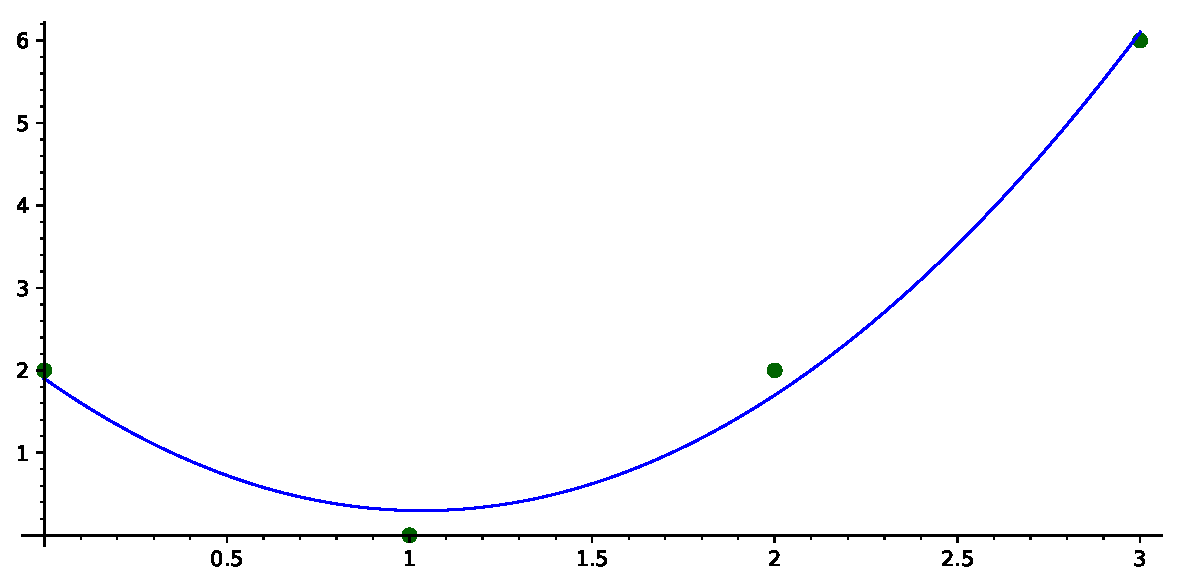
\includegraphics[width=5in]{leastsquares}
\]

\end{solution} 
\ee




\end{document}
